% !TeX document-id = {04d65a32-516d-4b85-9aaa-0206108e4b3a}
%!TEX program = xelatex 
% !BIB program = biber
\PassOptionsToPackage{table}{xcolor}
\documentclass[cn,10pt,citestyle=gb7714-2015, bibstyle=gb7714-2015]{elegantbook}
% citestyle=gb7714-2015 表示使用上标
% https://www.ctan.org/pkg/biblatex-gb7714-2015?lang=en


% 配色
% third: proposition
% 0, 160, 152   (green)
% 244, 105, 102  (cyan)
% 0, 174, 247    (blue)

% second:
% 175, 153, 8  (cyan)
% 230, 90, 7   (green)
% 255, 134, 24 (blue)



\title{运动生物力学}
\subtitle{开源湖工商经典之作}

\institute{OpenHUTB}
\date{\today}
\version{2.0}

\extrainfo{认识你自己。——古希腊德尔斐神庙墙上镌刻的箴言}

\setcounter{tocdepth}{3}

%\logo{logo-blue.png}
\cover{cover.jpg}

% 本文档命令
\usepackage{array}
% \usepackage{ctex}%加载ctex宏包,中文支持
%\usepackage{xr}

\newcommand{\ccr}[1]{\makecell{{\color{#1}\rule{1cm}{1cm}}}}

\definecolor{customcolor}{RGB}{32,178,170}
\colorlet{coverlinecolor}{customcolor}

\bibliography{reference}  % 关联参考文献文件 reference.bib

\begin{document}

\maketitle
\frontmatter

\chapter*{前言}

\markboth{Introduction}{前言}



\vskip 1.5cm

像诺亚方舟一样,开始一个巨大而愚蠢的项目……人们对你的看法完全无关紧要。


\vskip 0.5cm


%\vskip 1.5cm

\begin{flushright}
—— 鲁米\\
\end{flushright}


生物力学一直是我生活中积极而持久的力量。
小时候,在德尔普家,运动占据了我的生活。打棒球和长曲棍球让我充满活力,也喜欢跑步和滑雪。
高中毕业前,我只读过 2 本书:
一本是高山滑雪技术手册,另一本是跳远教练指南。
我有阅读障碍,只有这些简陋的生物力学手册,才值得我费力费力地去读,即使有些尴尬。


我在大学学习生物力学,学习如何在一次滑雪事故中髋部受伤后恢复行走能力。
我学习了所有关于生物力学的知识,几年后,当我能够行走自如,在斯坦福大学校园里一瘸一拐地走动时,我进入了研究生院。
我在研究生院学习了设计、机器人技术、神经科学和生物力学。
我觉得自己很适合帮助行动障碍人士,因为我对他们的困境感同身受,并且拥有深厚的工程设计和计算机科学背景,这在当时的生物医学研究中并不常见。
我有幸与费利克斯$\cdot$扎亚克一起学习生物力学,他对我的思考产生了很大的影响。



从斯坦福大学毕业后,我到西北大学和芝加哥康复研究所担任助理教授。
作为一名新教授,我希望分享我对生物力学的热爱,并教授一些能够帮助学生理解和分析肌肉和运动的原理。
这促成了我开设“运动生物力学”课程,这门课程我在西北大学和斯坦福大学已经讲授了大约30次。
本书涵盖了我在这门课程中教授的大部分内容。


通过阅读本书,你将学习生物力学的一些最重要的原理。
生物力学是一个运用物理学解释生物体运作方式的领域,从而帮助我们理解和珍惜生命。
生物力学是许多学科的核心,包括生物工程、机械工程、物理治疗、人体工程学、运动机能学和生物学。
我希望这些领域的学生能够从本书中受益。
我也为对神经科学、机器人技术、计算机科学和体育感兴趣的读者撰写本书。
除了学习生物力学原理外,你还将获得分析和模拟人体运动的技能;
这些技能将赋予你力量,让你为世界带来积极的改变。


许多刚开始学习生物力学的人分为 2 类:
一类是工程师,他们对生物学的语言感到困惑;
另一类是生物学家,他们对工程学的语言感到困惑。
这两种语言都很重要。
虽然它们经常被分开教授,但大自然并不在意人类在学科之间设置的界限。
本书的目的之一就是帮助你在精通这两门学科方面有一个良好的开端。
因此,我并不要求你事先具备任何生物学知识。


我确实需要假设读者对物理学有所了解,否则这本书会比现在长得多。
牛顿定律描述了从行星到人体的一切运动。
我们需要这些定律以及其他力学原理来分析人体运动,因此我假设读者已经学习过物理或工程学课程,具备力学方面的基础知识。
由于数学是力学的语言,我还假设读者掌握了微积分的基本概念,包括导数、积分和微分方程。
毕竟,力学的起点(牛顿第二定律)本身就是一个微分方程。


我的目标是写一本通俗易懂的书,用引人入胜、发人深省的例子来阐述生物力学的关键概念。
我写这本书并非为了综述文献。
关于生物力学的文章数以千计,引人入胜,也有很多优秀的综述文章;
我只引用了其中的一小部分。
我的目标是向生物力学的新手介绍生物力学,并帮助他们探索生物力学文献。
除了涵盖既定的原理外,我还重点介绍了一些将塑造该领域未来的重大理念,并阐述了如何践行这些理念,从而对科学、工程、艺术以及他人的生活产生积极影响。
如果您已经是生物力学领域的专家,我衷心希望您喜欢这本书,并发现它对您的教学大有裨益。


我希望为您提供解决实际问题的工具。
虽然本书没有印刷作业题,但我和我的同事开发了一个网站,其中包含许多有趣且具有挑战性的题目。
解决这些问题将大大扩展您的知识面。
您可以在 \href{biomech.stanford.edu}{biomech.stanford.edu} 在线找到这些问题,该网站还提供讲座幻灯片、教学大纲和其他欢迎您使用的资料。
您也可以在此网站上提供反馈。
请告诉我您喜欢哪些内容以及我可以如何改进本书。
本书包含大量数据,我和我的同事在 \href{simtk.org}{simtk.org} 上提供了其中的大部分数据。
我们建立这个网站是为了分享生物力学模型、软件和数据,我鼓励您使用并为之做出贡献。


这本书包含大量罕见汇集的信息,但内容并不全面。
我很少详细阐述神经系统在协调和控制运动中的作用,也没有讨论肌肉如何随着运动、废用或年龄而变化。
此外,我对骨骼、软骨和韧带的生物力学也进行了有限的讨论。
这些引人入胜的主题在其他书籍中都有详尽的阐述。


与汤姆$\cdot$内田和我的兄弟大卫$\cdot$德尔普一起撰写和绘制这本书是我职业生涯中最愉快、最有成就的合作之一。
大部分工作都是在我们家餐桌上的“聚会”中完成的。
我们的目标之一是用同一个声音写作。
汤姆和我合作得非常密切,以至于我们都无法告诉你是谁起草了这本书的句子。
这些故事来自我的经历,由于我曾多次教授运动生物力学课程,我们决定用我的风格来写;
然而,每一页都留下了汤姆的指纹。
如果您欣赏书中对力学概念表达的精准性,您可以为此感谢汤姆。
如果您和大多数人一样更喜欢书中的图片而不是文字,您可以感谢我的兄弟。
他是一位出色的艺术家,帮助我们创作了这本书,希望您会发现它是一本精美的书。


数学家兼才华横溢的作家达纳$\cdot$麦肯齐对整部手稿提供了详尽的评论和建议,极大地改进了本书。
读书不应该成为一件苦差事,而应该带给读者与作者同等的快乐。
达纳努力从那些隐藏着快乐的地方唤起这份快乐。
我非常感谢他这样做,我想你也会如此。


世界级生物力学家西尔维亚$\cdot$布莱姆克尔提供了第~\ref{chap:chap4}~至~\ref{chap:chap6}~章的早期草稿,其中包括一些关于图表和示例的精彩构思,她值得特别感谢。
我们还要感谢麻省理工学院出版社的莫莉$\cdot$西曼斯和马修$\cdot$阿贝特。
莫莉为本书的设计提供了创意,并负责了每一页的排版。
马修则对文本提出了宝贵的反馈,并逐字逐句地审校。



许多例子都出自我实验室的研究成果,我的合作者需要得到认可,为此,我在书中列举了一些合作者的名字,并在我们合著的论文中引用了其他合作者的名字。
美国国立卫生研究院为这项工作提供了支持,我非常感谢他们的支持。


其他朋友、同事、学生和导师也做出了宝贵的贡献,他们审阅了本书的初稿,与我合作撰写了一些论文,并从中汲取了灵感,或者向我解释了一些关键概念。
我要感谢以下几页图片中出现的各位,感谢他们的真知灼见和合作。
生物力学是一项团队运动,我很荣幸能与你们并肩作战。



我非常感谢在生物力学领域结识的众多朋友,他们一直是我生活中的一股积极力量。




\tableofcontents

\mainmatter





\chapter{第一步} \label{chap:chap1}

当时已是凌晨一点钟;雨点凄厉地拍打着窗玻璃,我的蜡烛快要燃尽了。
这时,借着半熄灭的微光,我看到那怪物睁着一只暗黄色的眼睛;它呼吸急促,四肢抽搐着。

\begin{flushright}
	——玛丽$\cdot$雪莱,《弗兰肯斯坦》(1818)\\
\end{flushright}


\begin{figure}[!htb]
	\centering
	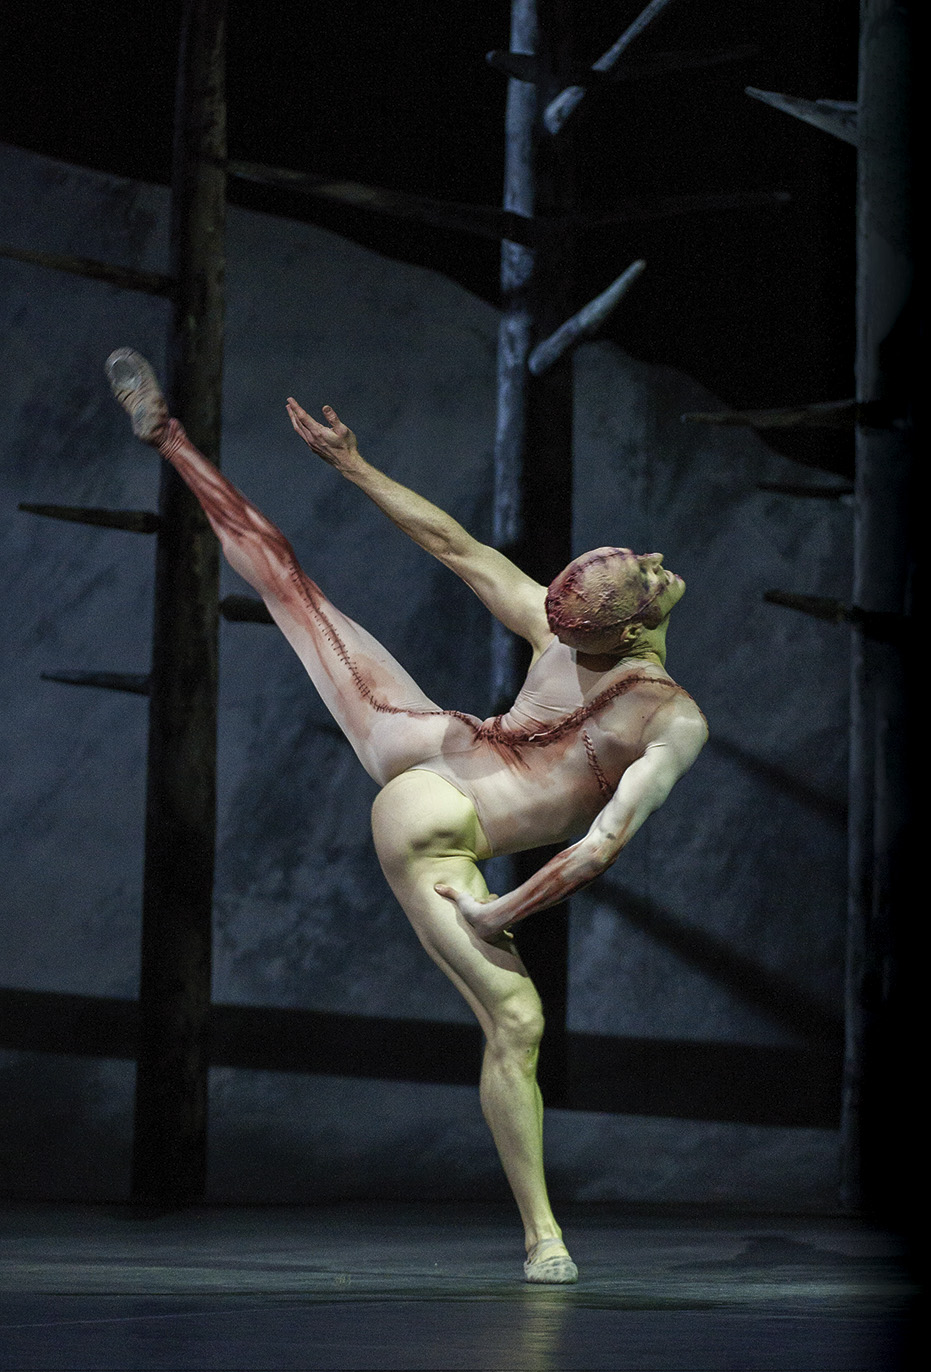
\includegraphics[width=0.5\linewidth]{chap1/1_0}
	% 加星号(*)表示不加编号
	\caption*{ \label{fig:1_0}}
\end{figure}

当玛丽$\cdot$雪莱写下那本让她名声大噪的哥特式小说时,全世界仍在为电的发现而兴奋不已——而路易吉$\cdot$加尔瓦尼的惊人发现——电刺激竟能使死青蛙的肌肉抽搐。
雪莱几乎可以想象,电流能使一个完整的生命体复活。


如今,距离伽伐尼的演示已过去两个世纪,肌肉电刺激技术对生活产生了深远的积极影响。
每个机场、学校和医院都安装了电除颤器,它们已经让成千上万的人的心脏重新跳动,而如果没有对心肌进行强力电击,这些人可能会死亡。
一项名为功能性电刺激的更先进的技术已被开发出来,它可以使各种瘫痪患者的肌肉恢复活力,从而改善他们的生活质量。


在功能性电刺激中,电极要么贴在皮肤上,要么植入瘫痪肌肉中,靠近支配这些肌肉的神经。
电脉冲通过电极传输到神经,进而引起相关肌肉收缩并产生力量。
肌肉电刺激使瘫痪患者在躯干和腿部肌肉得到适当激活和协调的情况下能够站立和行走。
2016年,几名脊髓损伤导致胸部以下瘫痪的患者参加了一项名为“Cybathlon”的全新国际自行车比赛。获胜者在不到3分钟的时间内骑行了750米。


功能性电刺激远不止向神经和肌肉输送电流那么简单。
对于健全人来说,神经系统协调着许多肌肉,使我们能够行走、跑步或骑自行车,就像指挥家协调管弦乐队的乐手一样。
当 Cybathlon 比赛的冠军在赛道上骑行时,多达 24 个通道的精确定时刺激能够被传送,以协调他原本瘫痪的肌肉产生的力量。
即使达到了这种复杂程度,结果也并非完美。
关于我们的肌肉如何协同工作以创作运动之乐,我们仍有许多需要学习的地方。


在本书中,我们将探索这首宏伟的交响曲。
我们将从力学的视角审视人类和动物的运动,以理解运动的生物力学。
我们将运用简单的概念模型来解答诸如为何行走和跑步是高效的运动方式、为何宇航员在月球上采取跳跃式步态,以及跑道和跑鞋如何提升运动表现并减少损伤等问题。
我们将深入研究肌肉的结构,直至其微观的动力产生机制,并精确观察电刺激如何促使肌肉收缩。
我们将描述用于生成运动模拟的复杂计算工具,从而使我们能够估算产生这种运动的肌肉力量。
这些模拟向我们展示了我们在行走、跑步或骑自行车时如何协调肌肉。
事实上,肌肉驱动的模拟对于Cybathlon金牌团队来说是一个宝贵的工具。


本书始终强调既定理论,为理解运动生物力学奠定基础,并涵盖计算机模拟、移动运动监测和可穿戴机器人等领域基于这些基础的创新。
许多近期的进展都由科幻小说所预见,并为我们展现未来新技术的雏形。
其中一些愿景或许如同唤醒弗兰肯斯坦的怪物般奇幻,而另一些则近在眼前。
无论如何,我们都在探索这个激动人心领域的潜力。






\section{我们为什么研究运动}

运动令人着迷,是生命的基础。
我们的身体功能多样,既能展现力量,又能展现灵巧。
运动对于维持身心健康至关重要。规律的体育锻炼有助于预防心脏病、癌症、骨质疏松症、肥胖症、糖尿病、抑郁症、焦虑症和其他严重疾病,然而,全球只有不到一半的人口能够充分活动以维持身心健康。
体育锻炼是一剂强效且廉价的良药,即使少量运动也能带来显著的健康益处。
在研究运动生物力学的过程中,我们致力于理解运动产生的生物结构和过程,并将这些知识应用于提高灵活性、体育锻炼能力和健康水平。


运动生物力学领域历史悠久。
如同人类的许多追求一样,推动其进步的动力源于改善生活的渴望,以及对环境和自身与生俱来的好奇心。
亚里士多德在公元前350年左右撰写了第一本探讨动物运动一般原理的著作,书名恰如其分地命名为《动物运动论》。
他和其他古希腊人认为,当肌肉被“气”(pneuma)——流经我们神经的“生命之气”——充气时,肌肉就会收缩。


此后,无数学者推动了该领域的发展,本书将介绍其中一些学者。
生物力学的先驱包括列奥纳多$\cdot$达$\cdot$芬奇(1452-1519),他绘制了数百幅详细的解剖图,并研究了肌肉骨骼系统的力学功能(图~\ref{fig:1_1})。
乔瓦尼$\cdot$博雷利(1608-1679)是第一个运用力学定律将肌肉施加的力与其在关节周围产生的力矩联系起来的人(图~\ref{fig:1_2})。
然而,博雷利仍然坚持经典观点,认为肌肉是通过气动、膨胀过程收缩的。
这一理论遭到了佛罗伦萨宫廷中博雷利的对手尼古拉斯$\cdot$斯坦诺(Nicolas Steno,1638-1686)的反驳,他指出肌肉在收缩时体积保持不变——我们将在第 4 章中研究这个悖论。
后来,路易吉$\cdot$加尔瓦尼(Luigi Galvani,1737-1798)发现了电信号能够引起肌肉收缩这一此前未被怀疑的能力,从根本上奠定了我们现代电生理学领域的基础。
最后,我不能不提一下埃德沃德$\cdot$迈布里奇(Eadweard Muybridge,1830-1904),他在距离我家约一公里(现在的斯坦福大学校园)的地方进行了早期的人类和动物运动摄影研究。迈布里奇的照片即使在今天看起来也令人着迷,它们是电影和生物力学史上的里程碑(图~\ref{fig:1_3})。
事实上,电影制作技术和生物力学科学仍在齐头并进。


\begin{figure}[!htb]
	\centering
	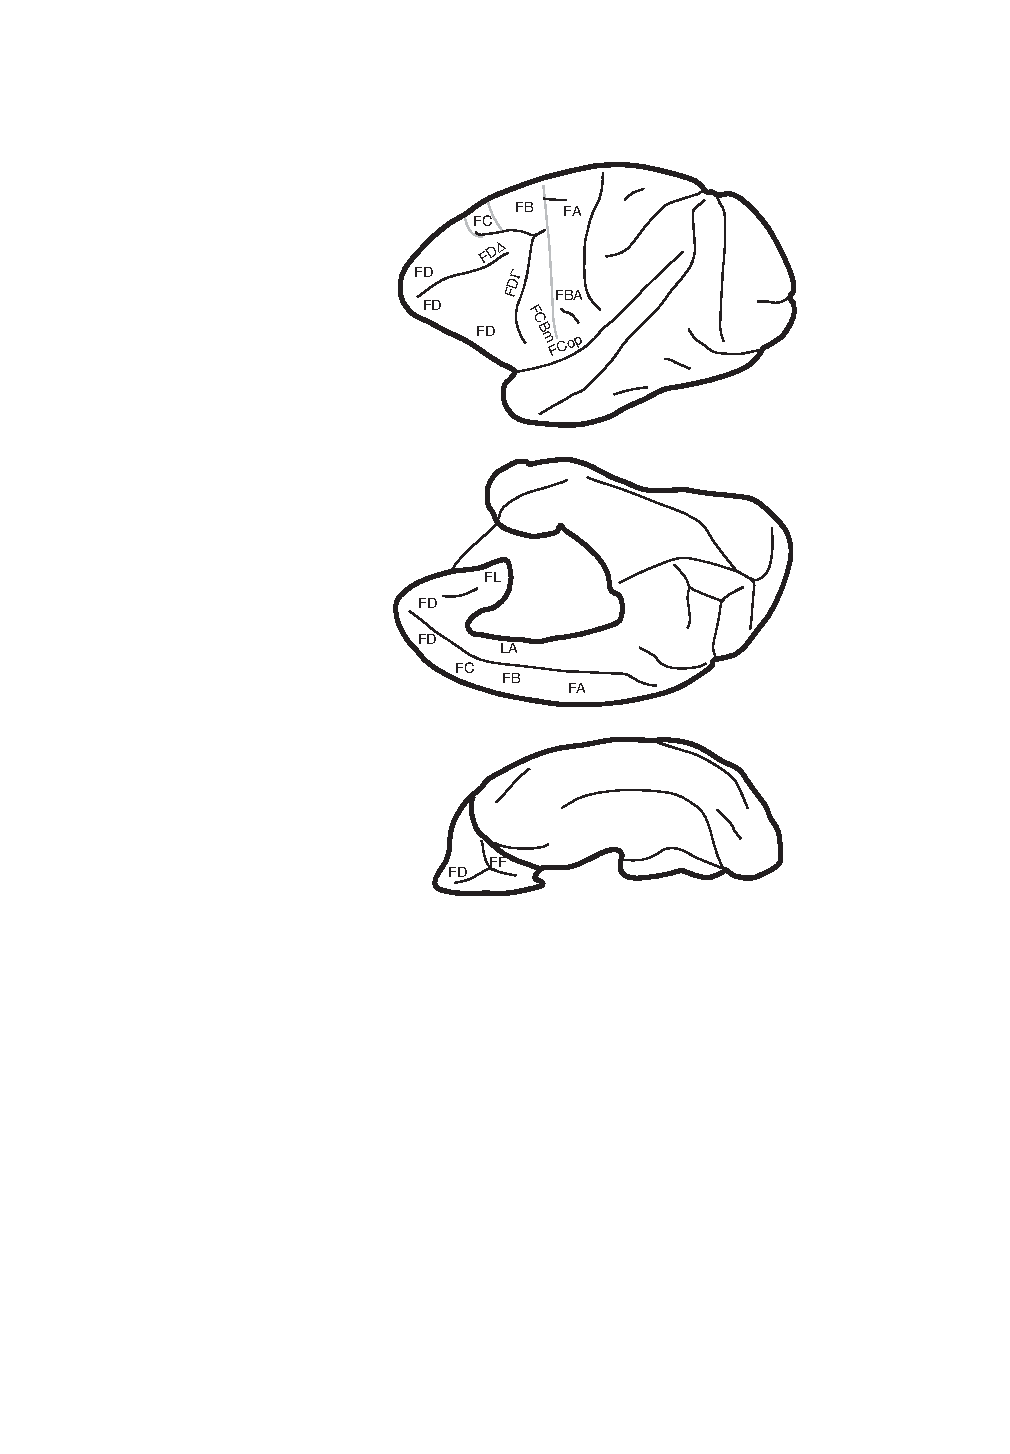
\includegraphics[width=0.75\linewidth]{chap1/1_1}
	\caption{列奥纳多$\cdot$达$\cdot$芬奇笔记本中的一页,展示了他的肌肉力线概念。
		图片由皇家收藏信托基金会提供。 \label{fig:1_1}}
\end{figure}


\begin{figure}[!htb]
	\centering
	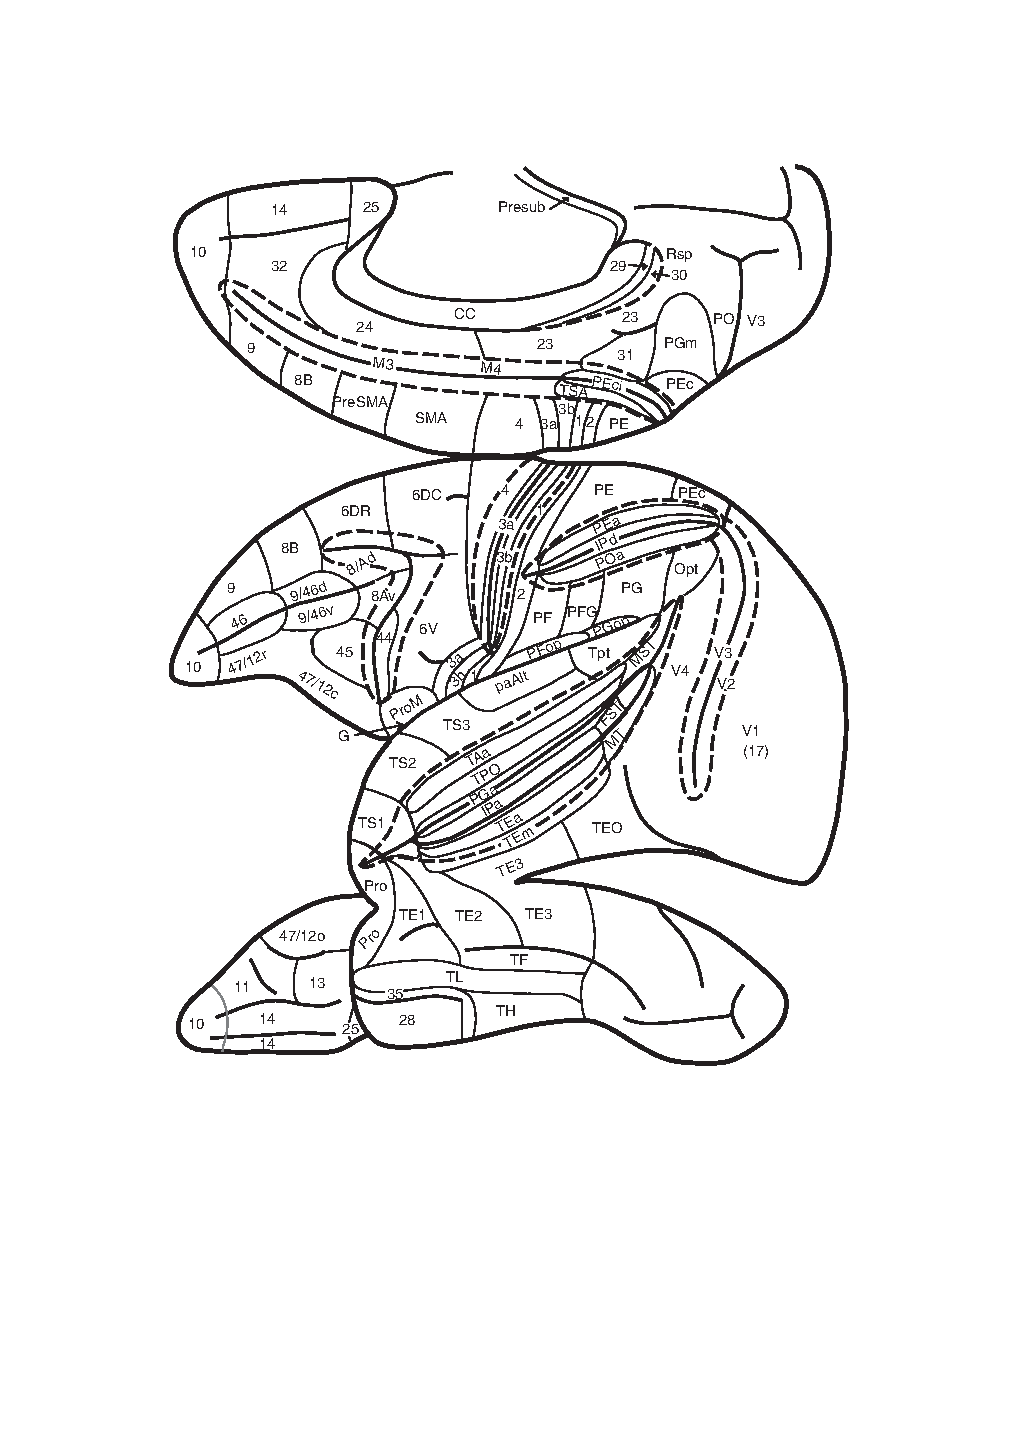
\includegraphics[width=0.75\linewidth]{chap1/1_2}
	\caption{乔瓦尼$\cdot$博雷利(Giovanni Borelli)对人体肌肉和关节的静态分析,他常被誉为生物力学之父。
		图片来自《动物运动》(De motu animalium)。 \label{fig:1_2}}
\end{figure}


\begin{figure}[!htb]
	\centering
	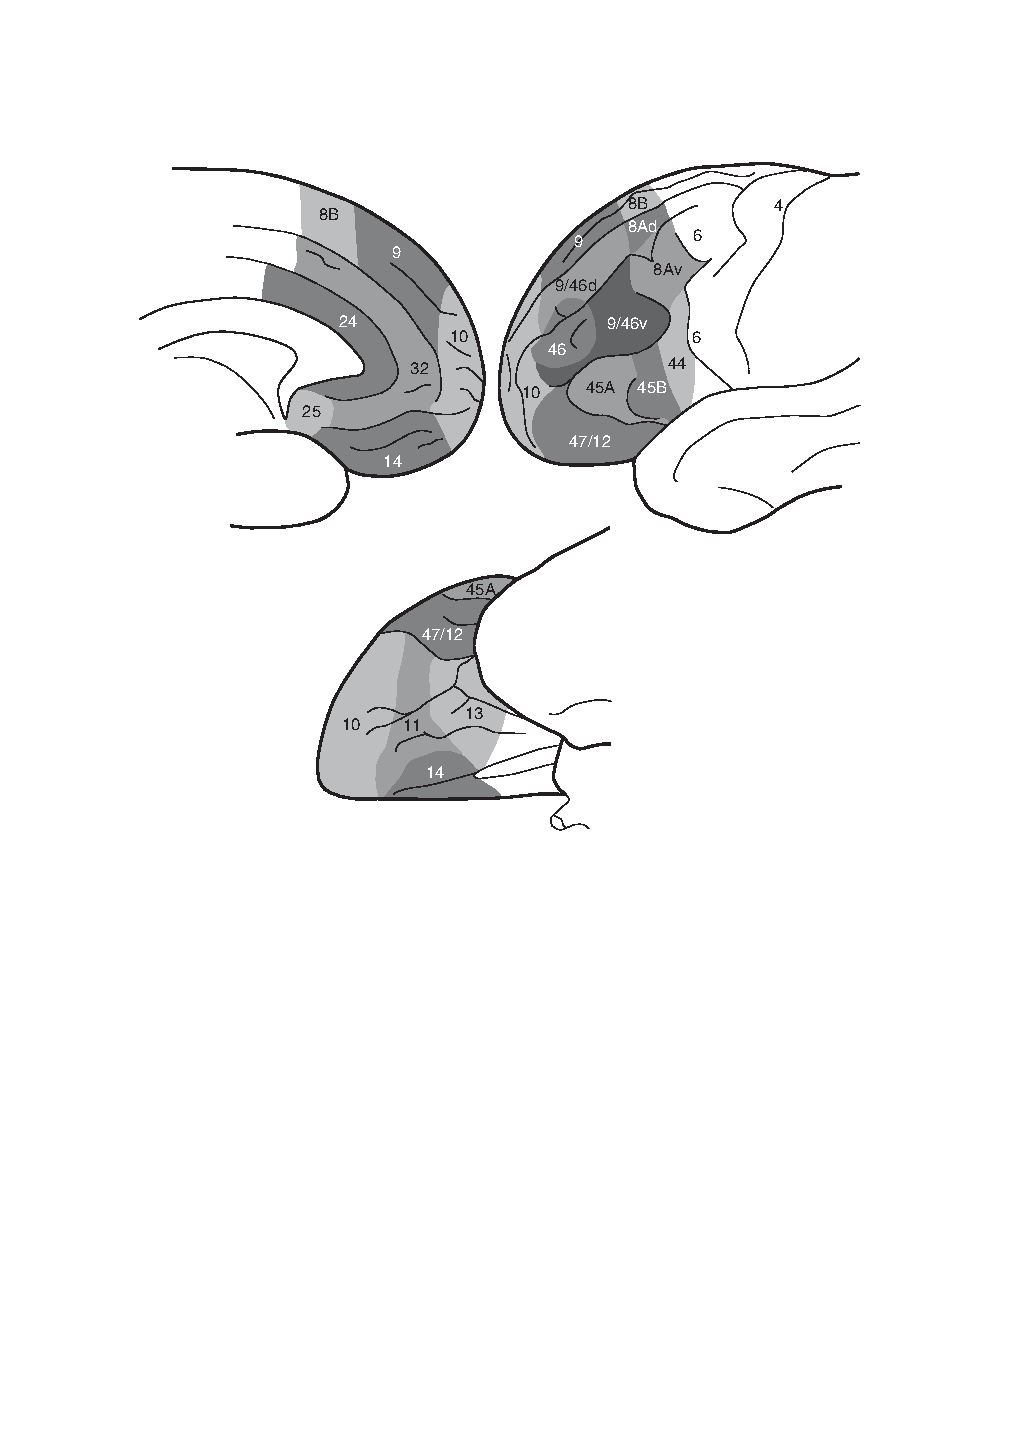
\includegraphics[width=1.0\linewidth]{chap1/1_3}
	\caption{动作捕捉先驱埃德沃德$\cdot$迈布里奇的一系列照片。
		图片由斯坦福大学提供。  \label{fig:1_3}}
\end{figure}


如今,生物力学是一个快速发展的多学科领域,汇聚了众多科学和工程领域的专家学者的通力合作。
生物学家利用生物力学的洞见来理解动物形态与功能之间的关系:
例如,蜥蜴如何跳跃并抓住墙壁(图~\ref{fig:1_4}),或者霸王龙是否能够奔跑(第~\ref{chap:chap3}~章)。
神经科学家研究大脑如何在运动过程中协调肌肉,以及这些神经回路在受伤和患病的情况下如何受到干扰。
外科医生可以使用生物力学模型来确定脑瘫患者是否能从肌腱延长手术中受益。
机器人专家正在发明日益精密的假肢(图~\ref{fig:1_5})和能够在危险环境中执行复杂任务的双足机器人。
运动科学家分析运动动作,例如“背越式跳高”(第~\ref{chap:chap9}~章),以了解如何提高运动表现并预防伤病。
计算机科学家和生物力学工程师开发新的算法和软件工具来模拟运动并从这些模拟中获得见解。


\begin{figure}[!htb]
	\centering
	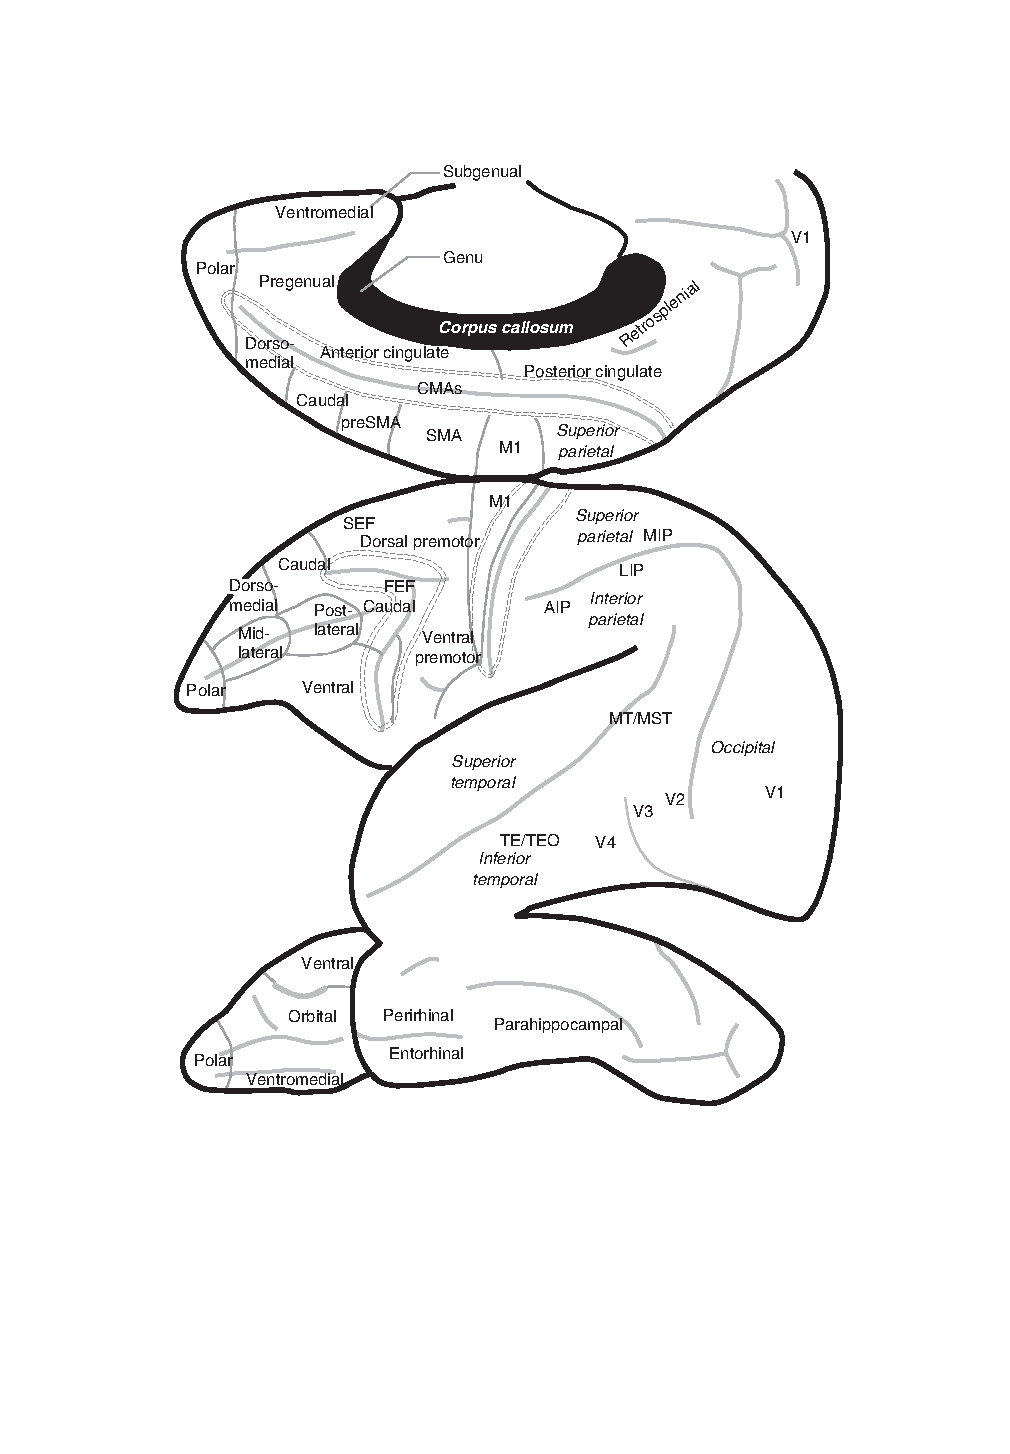
\includegraphics[width=1.0\linewidth]{chap1/1_4}
	\caption{红头鬣蜥在飞行过程中用尾巴控制身体方向。
		这只蜥蜴准备抓住右侧的垂直墙壁,它顺时针旋转尾巴,通过角动量守恒使身体保持垂直。
		图片由罗伯特$\cdot$富尔提供。 \label{fig:1_4}}
\end{figure}


\begin{figure}[!htb]
	\centering
	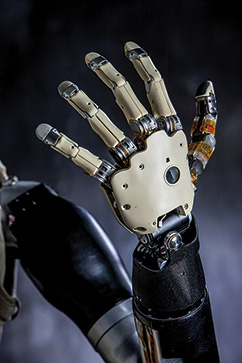
\includegraphics[width=0.5\linewidth]{chap1/1_5}
	\caption{功能强大的假肢如今触手可及。
		图片由约翰$\cdot$霍普金斯大学提供。 \label{fig:1_5}}
\end{figure}


生物力学甚至在科学领域之外也发挥着作用。电影制作人运用生物力学和动作捕捉技术,为游戏和电影创作计算机生成的图像,风格各异,从奇幻到逼真(图~\ref{fig:1_6})。
其成果将美感与科学的准确性完美结合,这在一两代人之前是难以想象的。


\begin{figure}[!htb]
	\centering
	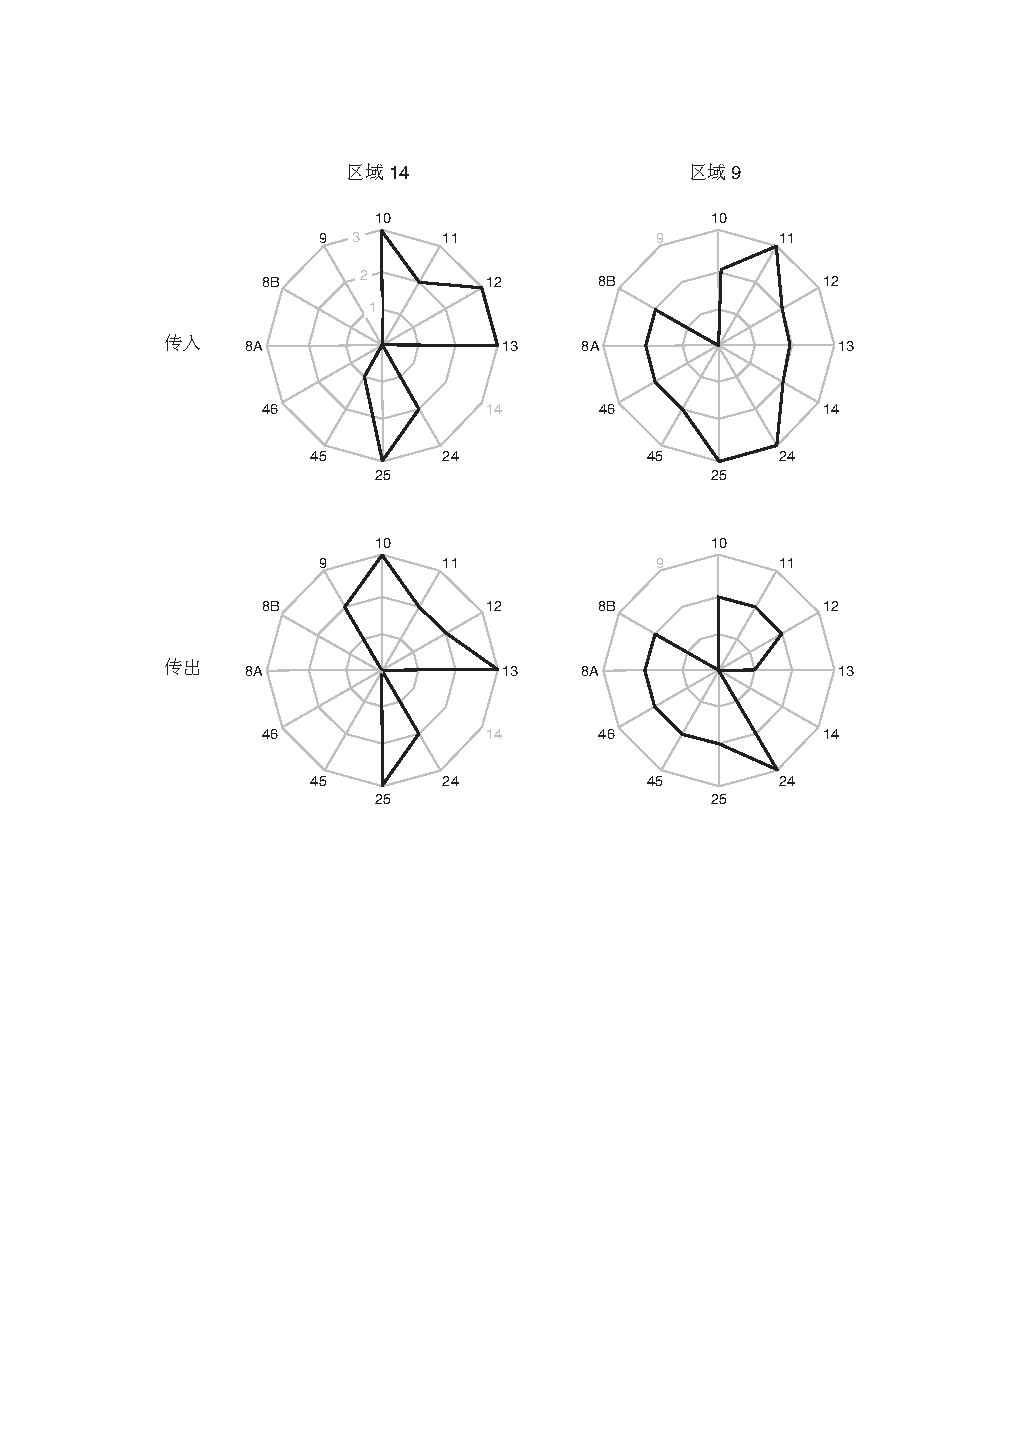
\includegraphics[width=1.0\linewidth]{chap1/1_6}
	\caption{图片来自电影《阿凡达》和行为艺术家詹$\cdot$斯塔福德。
		她的动作被动作捕捉技术记录下来,并制作成计算机生成的图像。
		图片由二十世纪福克斯公司提供。 \label{fig:1_6}}
\end{figure}


总的来说,这些努力极大地改善了我们的生活。
现在,我们可以根据保持健康所需的日常体力活动水平获得建议,并且我们可以使用有助于我们实现健身目标的工具。
装配线、办公家具和许多消费品都符合人体工程学设计,以提高舒适度并防止受伤。
一些产品和程序已被设计用于置换髋关节和膝关节,减轻疼痛并恢复数百万骨关节炎患者的功能。
动力外骨骼正在彻底改变中风后康复,并可以使瘫痪患者恢复运动能力。
帕金森病等运动障碍已通过深部脑刺激得到成功治疗,深部脑刺激是指植入电极向大脑特定区域传递电脉冲。
硬膜外刺激是一种激活脊髓神经回路的技术,最近已显示出帮助脊髓损伤患者恢复自主运动的潜力。
运动员正受益于旨在降低受伤风险并提高运动表现的设备和训练计划(图~\ref{fig:1_7})。


\begin{figure}[!htb]
	\centering
	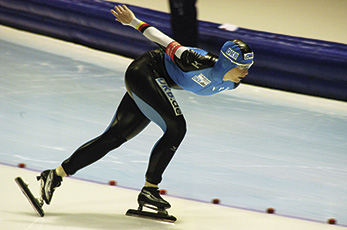
\includegraphics[width=0.6\linewidth]{chap1/1_7}
	\caption{生物力学研究有助于打造能够最大限度提升运动表现的运动器材。
		这款冰鞋的靴子和冰刀之间的铰链设计延长了冰刀与冰面的接触时间,从而增加了推进力的持续时间,从而提高了速度。
		图片由 McSmit 提供。 \label{fig:1_7}}
\end{figure}



\section{半机械人奥运会}


或许,更深入地观察一个引人注目的例子——“Cybathlon”(人机合体竞技),就能更好地理解生物力学的影响。
2016年,苏黎世联邦理工学院(ETH Zurich)教授罗伯特$\cdot$里纳(Robert Riener)组织了首届“Cybathlon”,这是一项将科学与体育进行创新性融合的运动。
与残奥会不同,这项运动的比赛项目侧重于日常任务。
例如,佩戴假肢的运动员比赛搬运物品、切面包、开罐子和晾衣服。
佩戴假肢的运动员比赛爬坡和上楼梯,同时保持杯子在碟子上保持平衡。
为了强调这项比赛关乎人类与科技的结合,参赛者被称为“飞行员”,而不是“运动员”。


在这场非传统的比赛中,最传统的体育项目是腿部瘫痪者自行车赛。
金牌被凯斯西储大学在罗纳德$\cdot$特里奥洛(Ronald Triolo)的科研领导下夺得。
该队的车手是马克·穆恩(Mark Muhn)(图~\ref{fig:1_8}),他在2008年的一次滑雪事故中脊髓受伤,胸部以下瘫痪。


\begin{figure}[!htb]
	\centering
	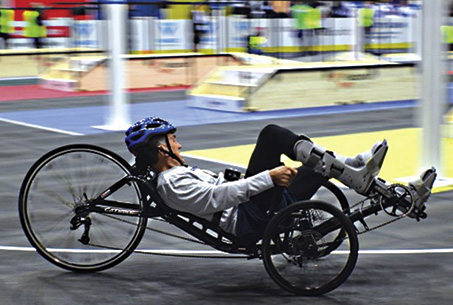
\includegraphics[width=0.6\linewidth]{chap1/1_8}
	\caption{马克$\cdot$穆恩参加 Cybathlon 比赛。
		图片由 Paul 和 Gabrielle Marasco 提供。 \label{fig:1_8}}
\end{figure}


凯斯西储大学的团队在功能性电刺激领域研究了四十年,并开发出了首批植入式神经肌肉刺激器。
特里奥洛相信,他们在植入电极方面的经验将成为制胜优势,因为其他团队正在使用通过皮肤传输电信号的电极。
植入电极可以更精准地刺激被激活的肌肉,从而产生更强烈的肌肉收缩。


该团队通过多种方式最大限度地提高了获胜的几率(McDaniel 等人,2017)。
他们购买了一辆卧式自行车,并将其拆解,去掉了所有不必要的重量。
他们让飞行员(最初有五名,其中两名被选中前往苏黎世)参加了强化训练计划。
我们最感兴趣的是他们使用的生物力学模型(图~\ref{fig:1_9})。


\begin{figure}[!htb]
	\centering
	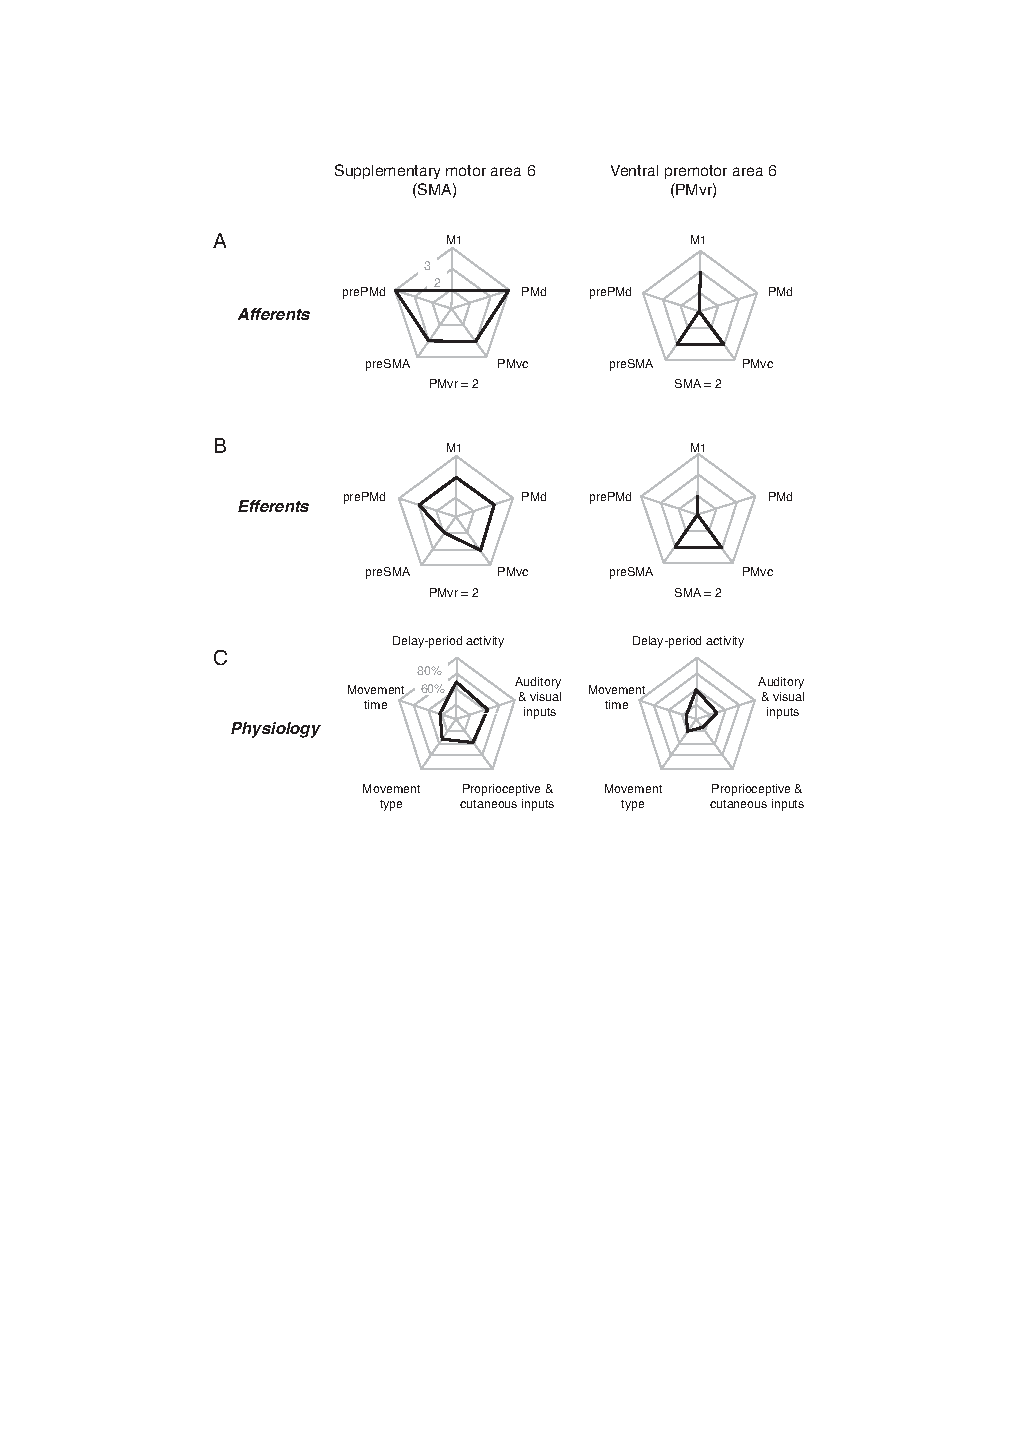
\includegraphics[width=1.0\linewidth]{chap1/1_9}
	\caption{用于调整肌肉兴奋模式以产生循环的肌肉驱动生物力学模型的示例。 \label{fig:1_9}}
\end{figure}


特里奥洛表示,这些模型与我们在本书后面描述的类似,在两个方面发挥了作用:
首先,它消除了“死胡同”(行不通的想法);
其次,它优化了提供给飞行员的电刺激模式。
每块腿部肌肉的每一次收缩都由一个外部控制装置(一个绑在飞行员腰间的盒子)控制。
为了安全起见,飞行员可以控制盒子的开关。


为了获得刺激模式,研究小组从文献中获取了自行车运动的生物力学模型,并根据每位骑手的特点进行了定制。
定制非常重要,因为瘫痪后肌肉的特性会发生变化,而可以通过刺激激活的肌肉数量很少,所以适用于健全骑手的激活模式可能不适用于脊髓损伤患者的刺激驱动踩踏。
Musa Audu 带头为每位骑手建模和定制刺激模式,并采用第~\ref{chap:chap10}~章中描述的技术来估计每块肌肉激活的时间和强度。
值得注意的是,刺激模式在比赛期间从未改变。
当骑手的肌肉疲劳时,他的腿会保持以相同的速率抽动,但它们无法用那么大的力气推动,所以骑手必须换挡才能保持自行车前进。


事实上,飞行员之所以会很快感到疲劳,是因为功能性电刺激并不像大脑发出的自然信号那样募集肌肉纤维。
我们将在第~\ref{chap:chap4}~章中回顾这一现象,但现在只需说明,大多数自然发生的运动都是通过首先募集“慢肌”纤维(相对较小且抗疲劳),然后是“快肌”纤维(产生较大力量但很快疲劳)产生的。
然而,电刺激以相反的顺序募集肌肉纤维。
由于这种“反向募集”,飞行员在开始训练时几乎无法让摩托车持续行驶超过一分钟。



但意想不到的事情发生了——相比于单调乏味的固定自行车,飞行员们更喜爱比赛用自行车带来的户外锻炼。
而且运动训练可以增强瘫痪的肌肉。在飞行员们积极进取的激励下,经过5个月的训练,他们能够坚持骑车参加3分钟的比赛。
特里奥洛表示,他希望在未来几年找到一种技术解决方案来解决招募逆转问题,但在2016年,只有一个解决方案:“让我们的飞行员尽情锻炼”。
而且,这个方案真的奏效了!
在苏黎世,穆恩以2分58秒的成绩完成了750米的比赛,并夺得了金牌。


Cybathlon 的经历改变了 Muhn 的人生,或许更令人惊讶的是,它改变了 Triolo 的研究。
Triolo 说,以前他们的康复方法是任务导向的。
他们专注于让志愿者站立、行走或进行日常生活活动,比如穿衣和做饭。
但当他们的参与者在户外骑自行车,并开始在锻炼的同时享受乐趣时,一切都改变了。
他们锻炼得更多,这对他们康复的各个方面都产生了巨大的回报,包括提升了他们的自尊心。
当一名骑手在公共道路上骑自行车时,另一个骑手追上他并说:“轮子真漂亮。”
这几乎是陌生人第一次将他视为一个拥有酷炫自行车的人,而不是一个残疾人。



\section{研究运动的工具}

我写这本书的目标之一是让你熟悉我的团队和其他人员开发的肌肉驱动生物力学模型。重要的是要意识到这些模型是基于实验数据的。让我们来看看我们收集的数据类型。



分析运动的一种常用技术是在研究实验室和诊所录制个体的视频。
许多此类记录都是通过红外摄像机获得的,这些摄像机可以追踪贴在皮肤上的标记物,类似于电影制作中使用的技术(图~\ref{fig:1_10})。
最近,不需要标记物的运动捕捉技术变得越来越流行。
基于视频的系统已经广泛应用,但这些系统的普及程度已被惯性测量单元 (IMU) 所取代,IMU 现已集成到智能手机、可穿戴活动监测器和服装中。
IMU 能够在自然环境中长时间收集运动数据(速度和加速度),这对于监测病情进展和制定治疗方案非常有价值。
低成本活动监测器中 IMU 的普及也使得对全球数百万个体进行大规模研究成为可能(图~\ref{fig:1_11})。


\begin{figure}[!htb]
	\centering
	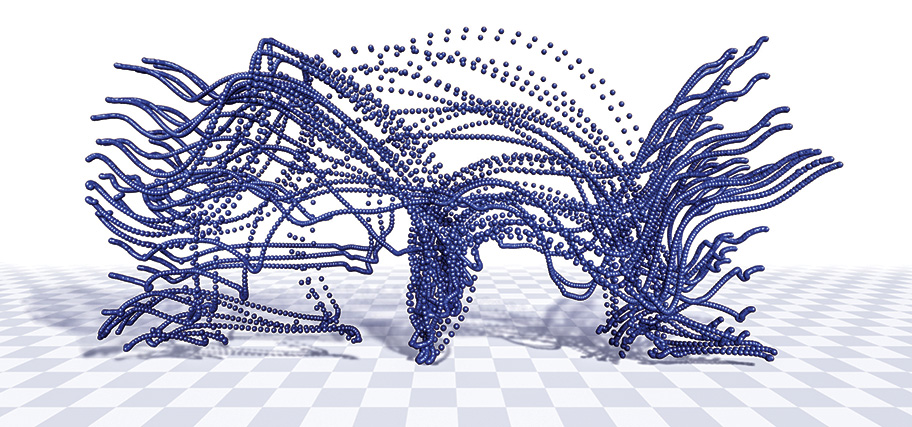
\includegraphics[width=1.0\linewidth]{chap1/1_10}
	\caption{前手翻(时长 2.9 秒)期间,贴在皮肤上的标记物轨迹。
		受试者最初站立(最左侧),然后向前跳跃,双手撑地翻身(中间),双脚落地,然后跳了一跳恢复平衡(最右侧)。
		球体间距越大,表示标记物移动速度越快。
		数据来自 ACCAD (2018)。 \label{fig:1_10}}
\end{figure}


\begin{figure}[!htb]
	\centering
	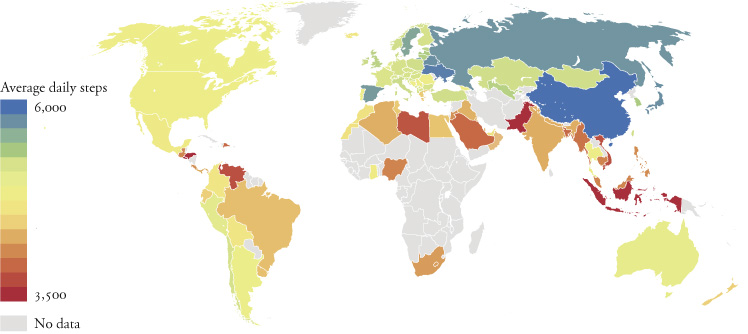
\includegraphics[width=1.0\linewidth]{chap1/1_11}
	\caption{717,527 名受试者超过 6800 万天的智能手机活动数据揭示了 111 个国家/地区的体力活动差异。
		图片改编自 Althoff 等人(2017 年)的研究,这是全球规模最大的体力活动调查。 \label{fig:1_11}}
\end{figure}


在实验室或诊所进行实验时,除了运动捕捉系统外,还可能涉及多种专用设备。
我们经常使用测力板来测量脚和地面之间的力。在步行和跑步研究中,使用跑步机很方便,因为受试者可以保持在运动捕捉系统能够精确测量的范围内。
一些跑步机还配备了测量地面反作用力的仪器。
肌电图用于测量各种肌肉活动的时间和强度。
我们可以监测跑步者的呼吸,测量消耗的氧气量和产生的二氧化碳量,以估算跑步所需的代谢能量。
磁共振成像和荧光透视成像等成像技术的普及使我们能够看到运动中的动物或人体内部,为可视化和测量运动提供了强有力的工具。


概念模型可以成为强大的分析工具,正如我们将在本书中看到的。
例如,第~\ref{chap:chap2}~章和第~\ref{chap:chap3}~章展示了一个简单的摆模型如何为我们合理地模拟行走,而一个质量弹簧模型如何为我们提供关于跑步的重要见解。
一个能够完成任务的简单模型几乎总是比一个更复杂的模型更受欢迎,后者提供了类似的实用性,但构建和理解起来更困难。
当然,并非所有复杂现象都能用简单的力学模型来表示。
正如我们将在第~\ref{chap:chap11}~章和第~\ref{chap:chap12}~章中看到的,肌肉驱动的模拟是强大的工具,可以填补第~\ref{chap:chap2}~章和第~\ref{chap:chap3}~章中简单模型所缺失的许多细节。


计算机模拟可以计算无法直接测量的量并预测假设场景中的运动,从而对实验进行补充。
模拟有助于理解例如难以通过实验研究的损伤。我们还可以估算导致观察到的运动的肌肉力量,以及关节负荷、肌腱应变和其他无法测量的量。
在正向动态模拟中,我们规定一块或多块肌肉的神经激活模式,然后预测肌肉骨骼模型的最终运动(图~\ref{fig:1_12})。
需要实验数据来开发和测试用于运动模拟的肌肉骨骼动力学数学模型,并评估模拟反映现实的程度。


\begin{figure}[!htb]
	\centering
	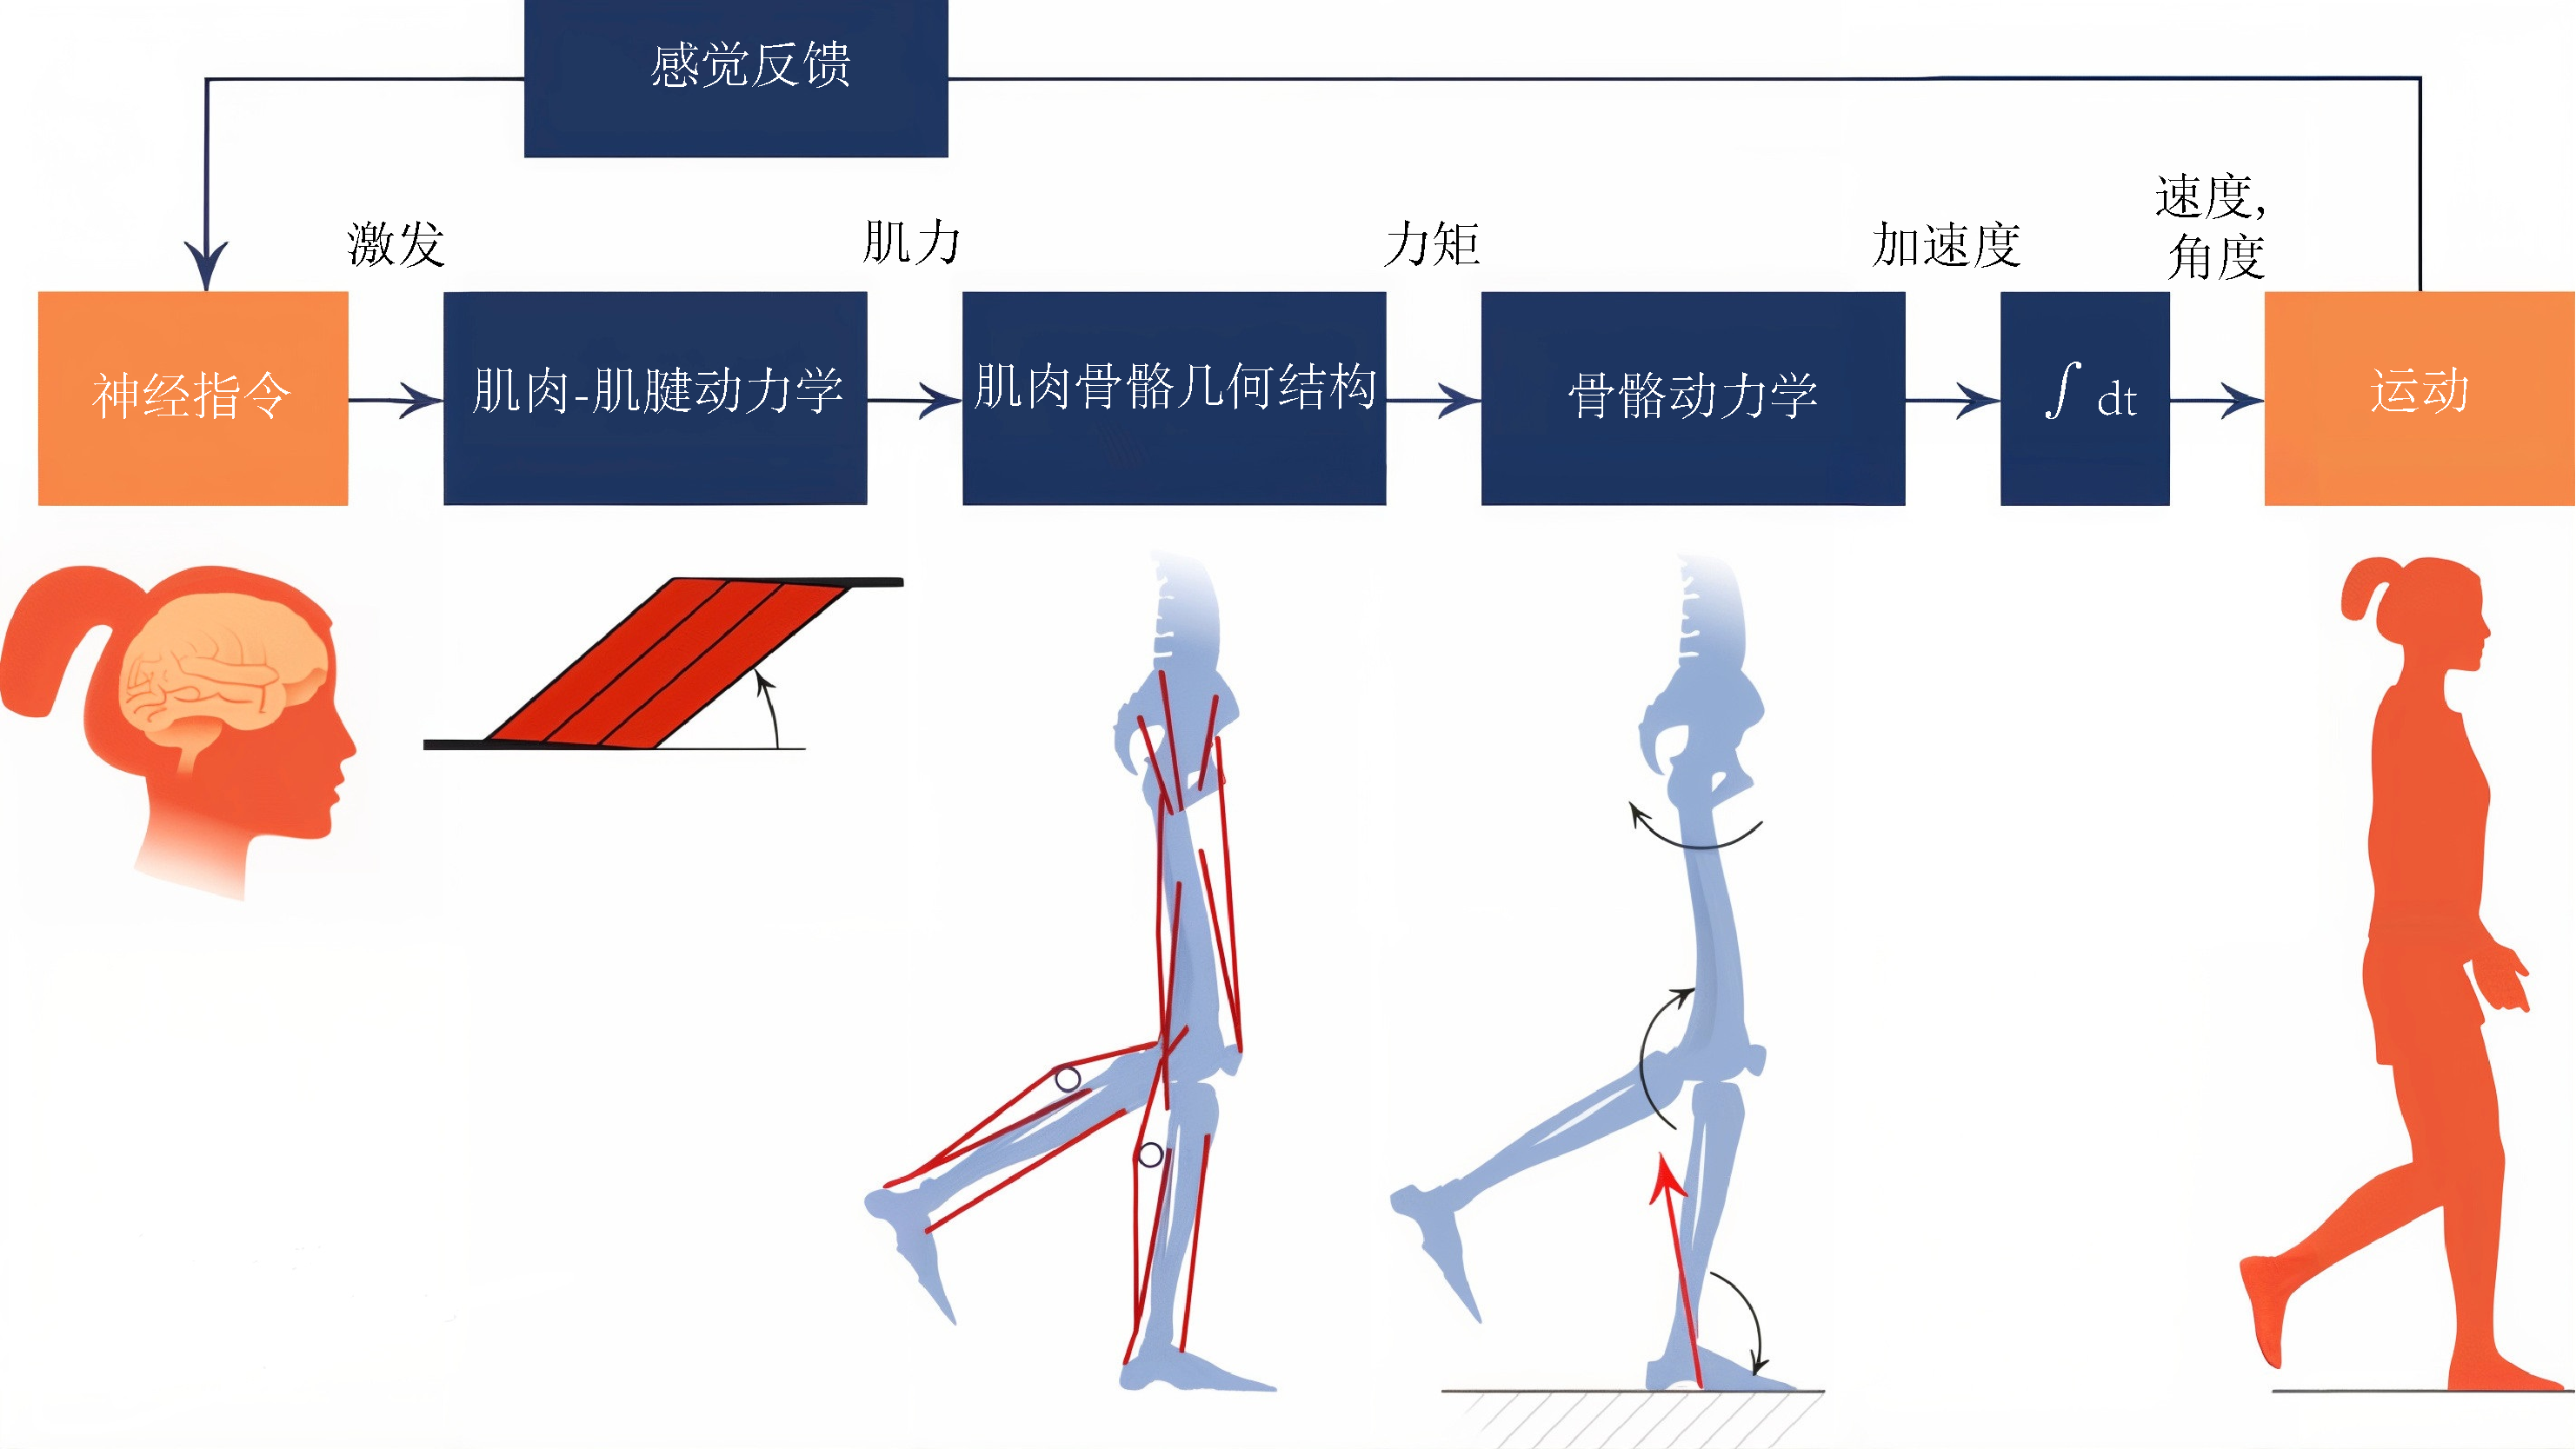
\includegraphics[width=1.0\linewidth]{chap1/1_12}
	\caption{典型的正向动态模拟的要素。
		运动源于神经、肌肉、骨骼和感觉系统的复杂协调。
		这些系统的计算模型使我们能够预测和分析人类和动物的运动。 \label{fig:1_12}}
\end{figure}


当我们测量了测试对象的运动并希望将这些数据转化为有意义的见解时,通常会使用逆过程,例如,肌肉必须产生哪些力才能产生测量到的运动。
为此,我们需要进行逆动力学分析,这是一种将实验数据与肌肉骨骼模型相结合的常见分析策略。
第一步是使用身体的生物力学模型,将标记位置的测量值(如图~\ref{fig:1_10}~所示)通过称为逆运动学的过程转换为关节角度(图~\ref{fig:1_13})。
关节角度根据时间进行微分,以估计关节角速度和加速度,然后将其与施加于身体的外力测量值结合使用,以估计关节力矩。
然后,将生物力学模型与优化算法结合使用,以估计肌肉力量。
我们将这种策略称为逆分析,因为运动测量值可用于推断产生这些运动必须存在哪些力。


\begin{figure}[!htb]
	\centering
	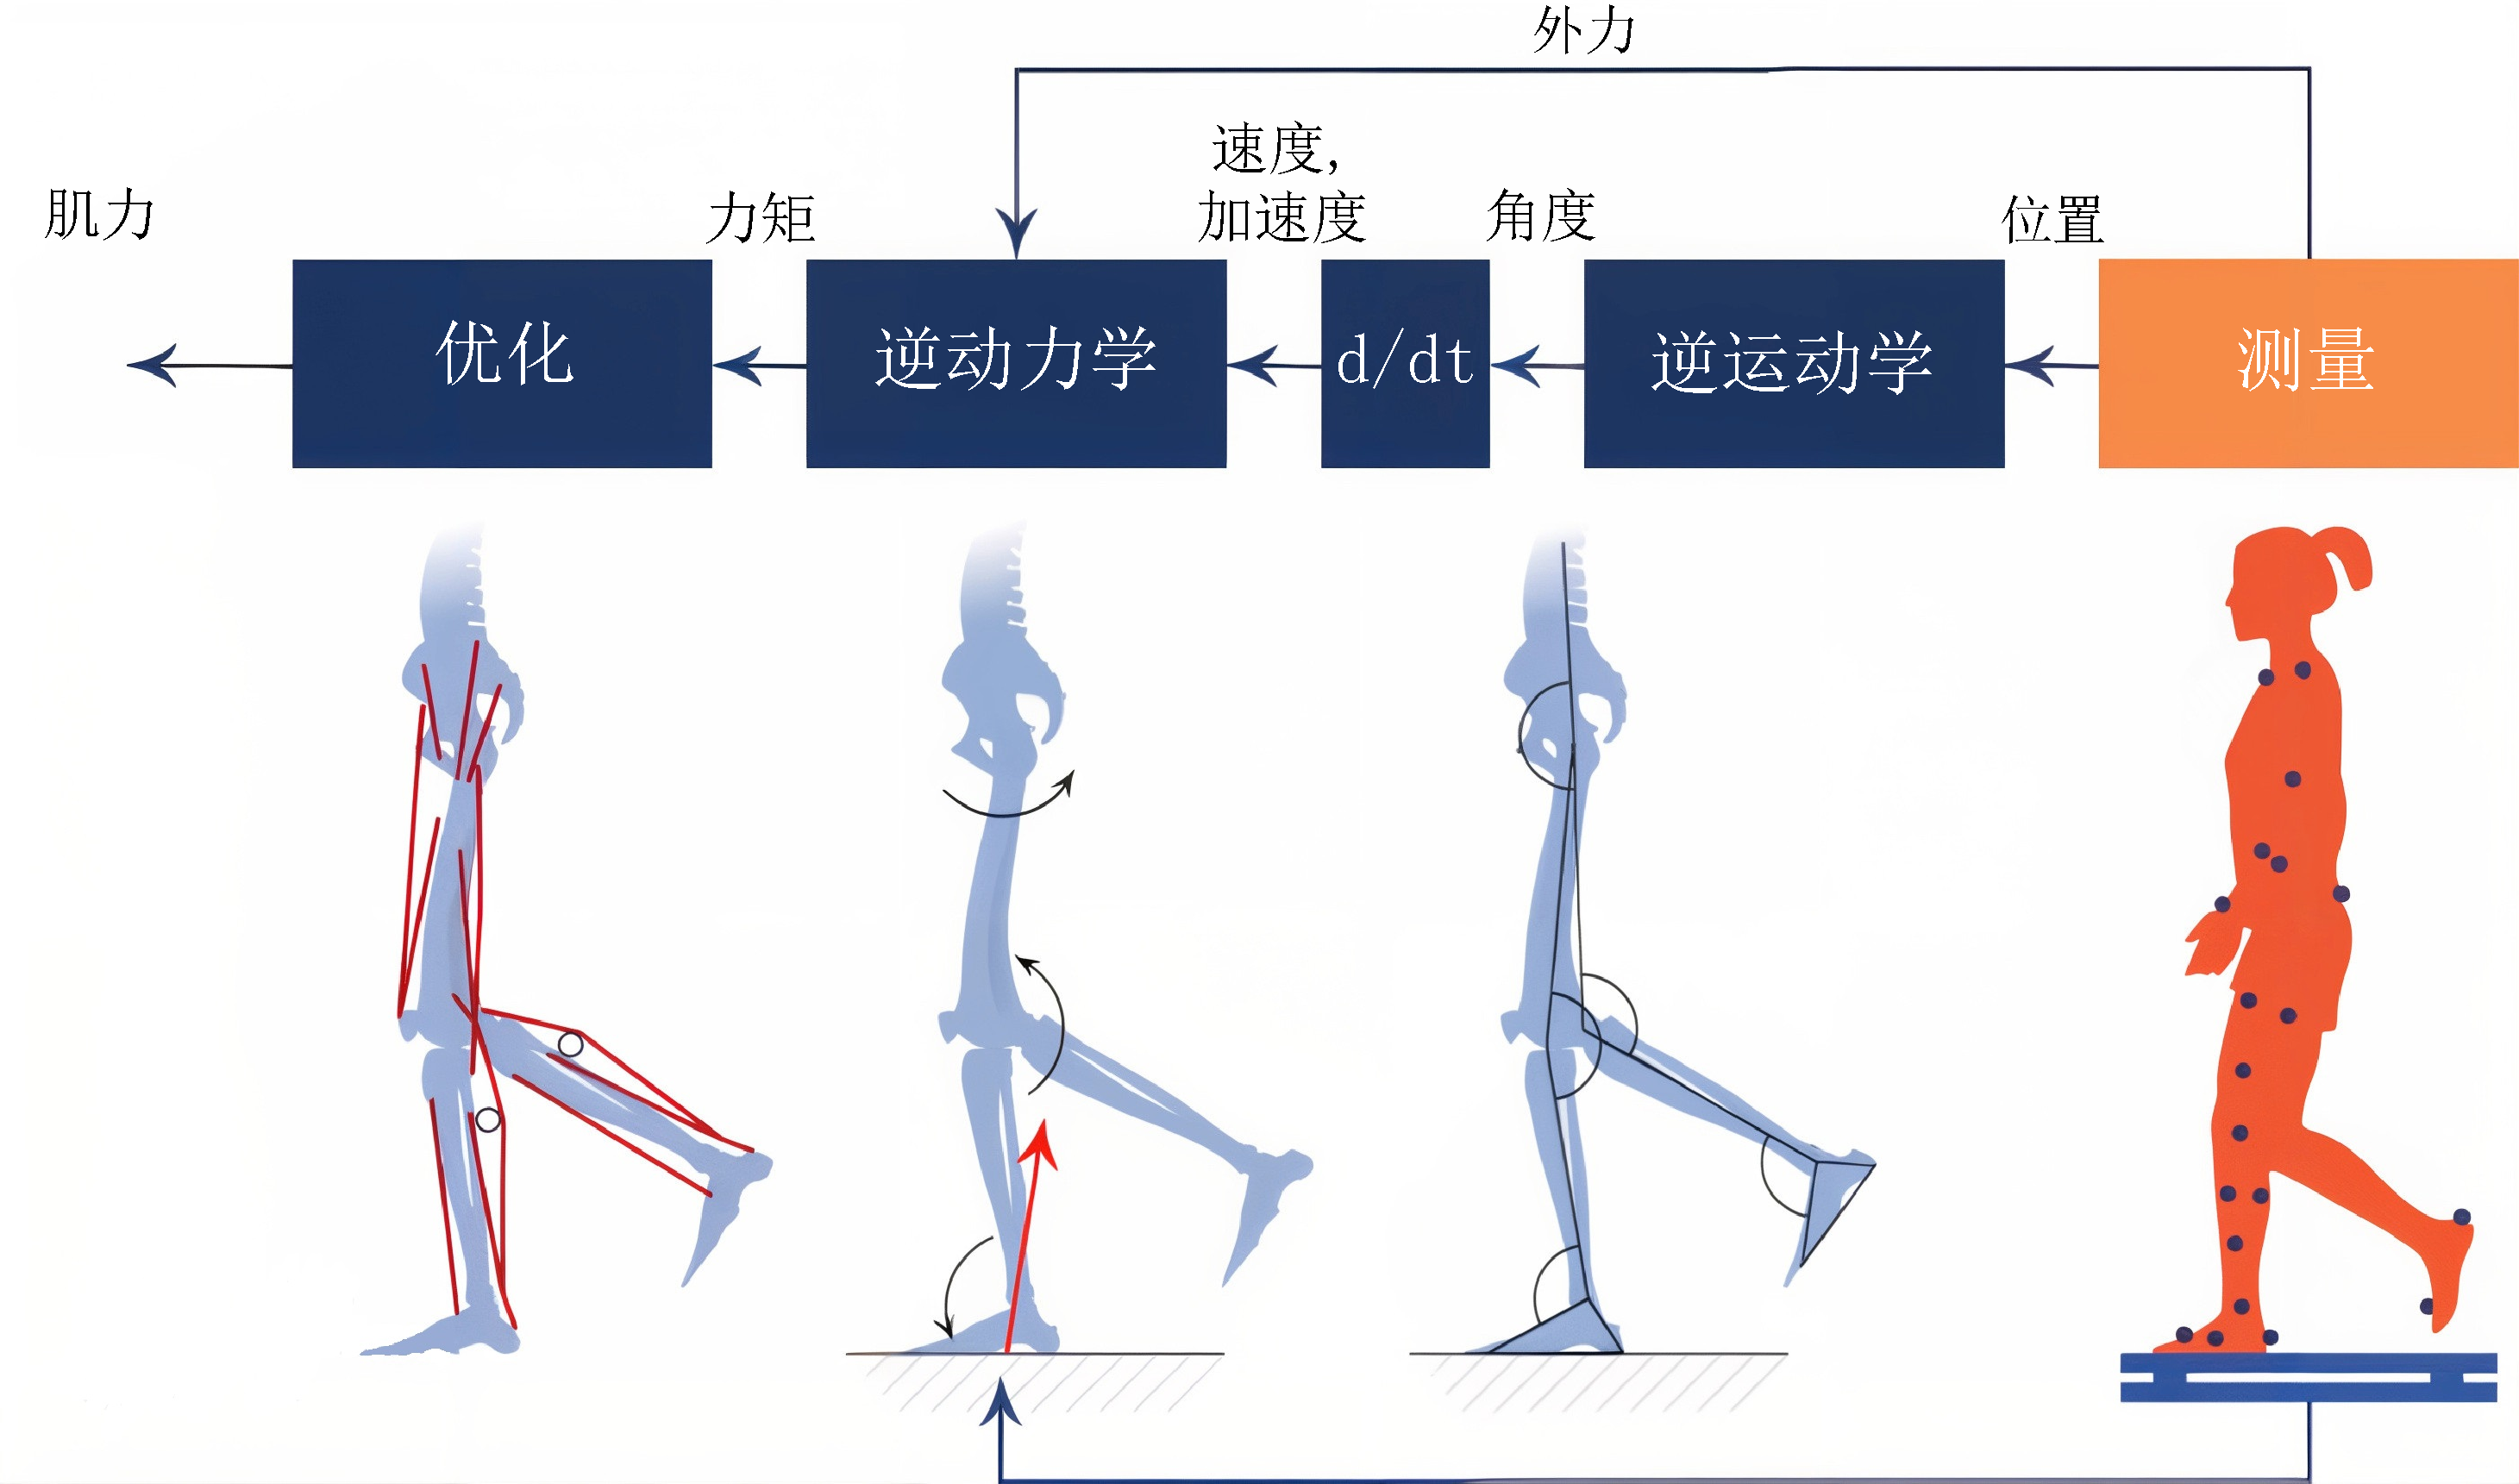
\includegraphics[width=1.0\linewidth]{chap1/1_13}
	\caption{典型逆动力学分析的要素。
		分析从测量标记轨迹和外力(右)开始,并使用生物力学模型估算身体各节段和关节的角度、速度和加速度。
		逆动力学模型和优化程序可估算关节力矩和肌肉力量。 \label{fig:1_13}}
\end{figure}




\section{本书概述}

在接下来的章节中,我们将首先使用简单的概念模型研究人类两种常见的运动形式——行走和跑步。
然后,我们将通过研究骨骼肌的生物学和结构、其与肌腱的动态相互作用以及肌肉如何产生驱动骨骼的力量来探索运动的产生。
接下来,我们将研究用于分析运动的模型和算法。
我们将演示如何从运动捕捉数据和生物力学模型中计算关节角度、关节力矩​​和单个肌肉的力量。
最后,我们将综合这些概念来研究肌肉在行走和跑步过程中的作用,并就我对该领域未来发展方向的一些看法进行总结。
如图~\ref{fig:1_14}~所示,本书的内容被安排成四个部分,我鼓励读者以这种方式来理解本书。
因此,第~\ref{chap:chap4}~章(第二部分的开头)并非第~\ref{chap:chap3}~章的续篇,但第~\ref{chap:chap5}~章无疑延续了第~\ref{chap:chap4}~章的篇幅。
如果您记住这一点,本书的内容将对您更有意义。


\begin{figure}[!htb]
	\centering
	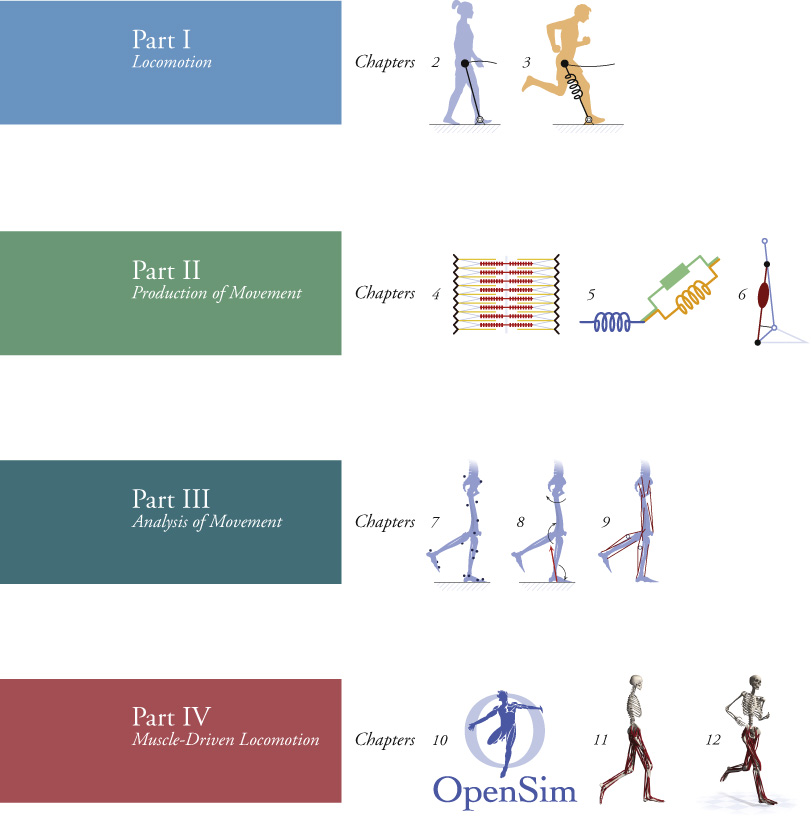
\includegraphics[width=1.0\linewidth]{chap1/1_14}
	\caption{本书的组织结构。 \label{fig:1_14}}
\end{figure}



虽然我们主要关注人类的运动,但我们所描述的基本概念也可用于理解动物和机器人的运动。
本书涵盖的内容将帮助您理解精彩纷呈、内容丰富的科学文献,这些文献对众多主题进行了详尽的分析,而一本书根本无法涵盖所有​​这些主题。


\section{运动语言}

我想解释一下你需要了解哪些知识才能充分利用本书。
汤姆和我为熟悉某些工程基础知识的读者编写了本书。
数学和力学为分析运动提供了精确的框架,我们假设读者对向量和矩阵有基本的了解。
我们进一步假设读者熟悉自由体运动图、推导运动方程以及如何求解简单系统的运动方程。
如果你不熟悉这些主题,你应该准备好在遇到它们时花一些额外的时间去学习。


在生物学方面,了解人体解剖学和生理学背景会有所帮助,但并非必需。
对于不熟悉解剖学的读者,以下图表展示了本书将要用到的术语。这些术语包括解剖平面和方向(图~\ref{fig:1_15})、关节运动(图~\ref{fig:1_16}~和图~\ref{fig:1_17})以及主要骨骼和肌肉(图~\ref{fig:1_18}~和图~\ref{fig:1_19})。
这些术语乍一看可能令人望而生畏,但花几分钟时间研究这些图表并学习这些术语,对你大有裨益。


\begin{figure}[!htb]
	\centering
	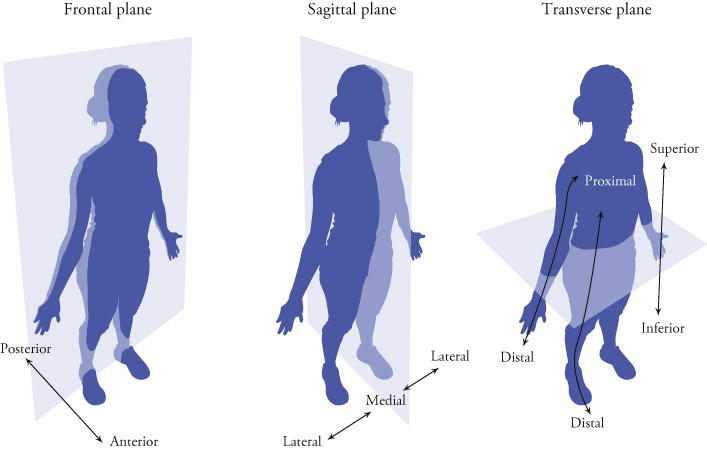
\includegraphics[width=1.0\linewidth]{chap1/1_15}
	\caption{人体的解剖平面和方向。 \label{fig:1_15}}
\end{figure}


\begin{figure}[!htb]
	\centering
	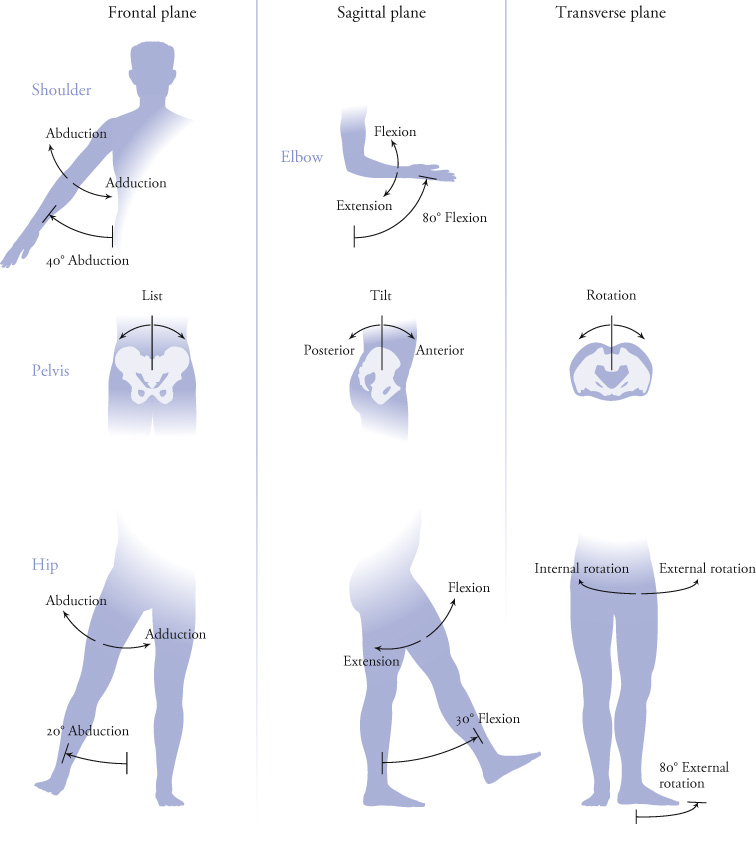
\includegraphics[width=1.0\linewidth]{chap1/1_16}
	\caption{肩部、肘部、骨盆和臀部在额状面(左)、矢状面(中)和横状面(右)的运动。 \label{fig:1_16}}
\end{figure}


\begin{figure}[!htb]
	\centering
	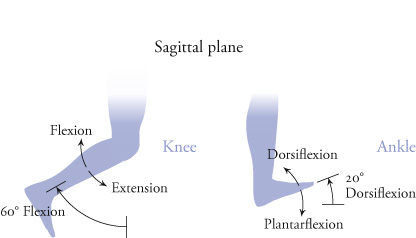
\includegraphics[width=0.75\linewidth]{chap1/1_17}
	\caption{膝盖和脚踝在矢状面上的运动。 \label{fig:1_17}}
\end{figure}


\begin{figure}[!htb]
	\centering
	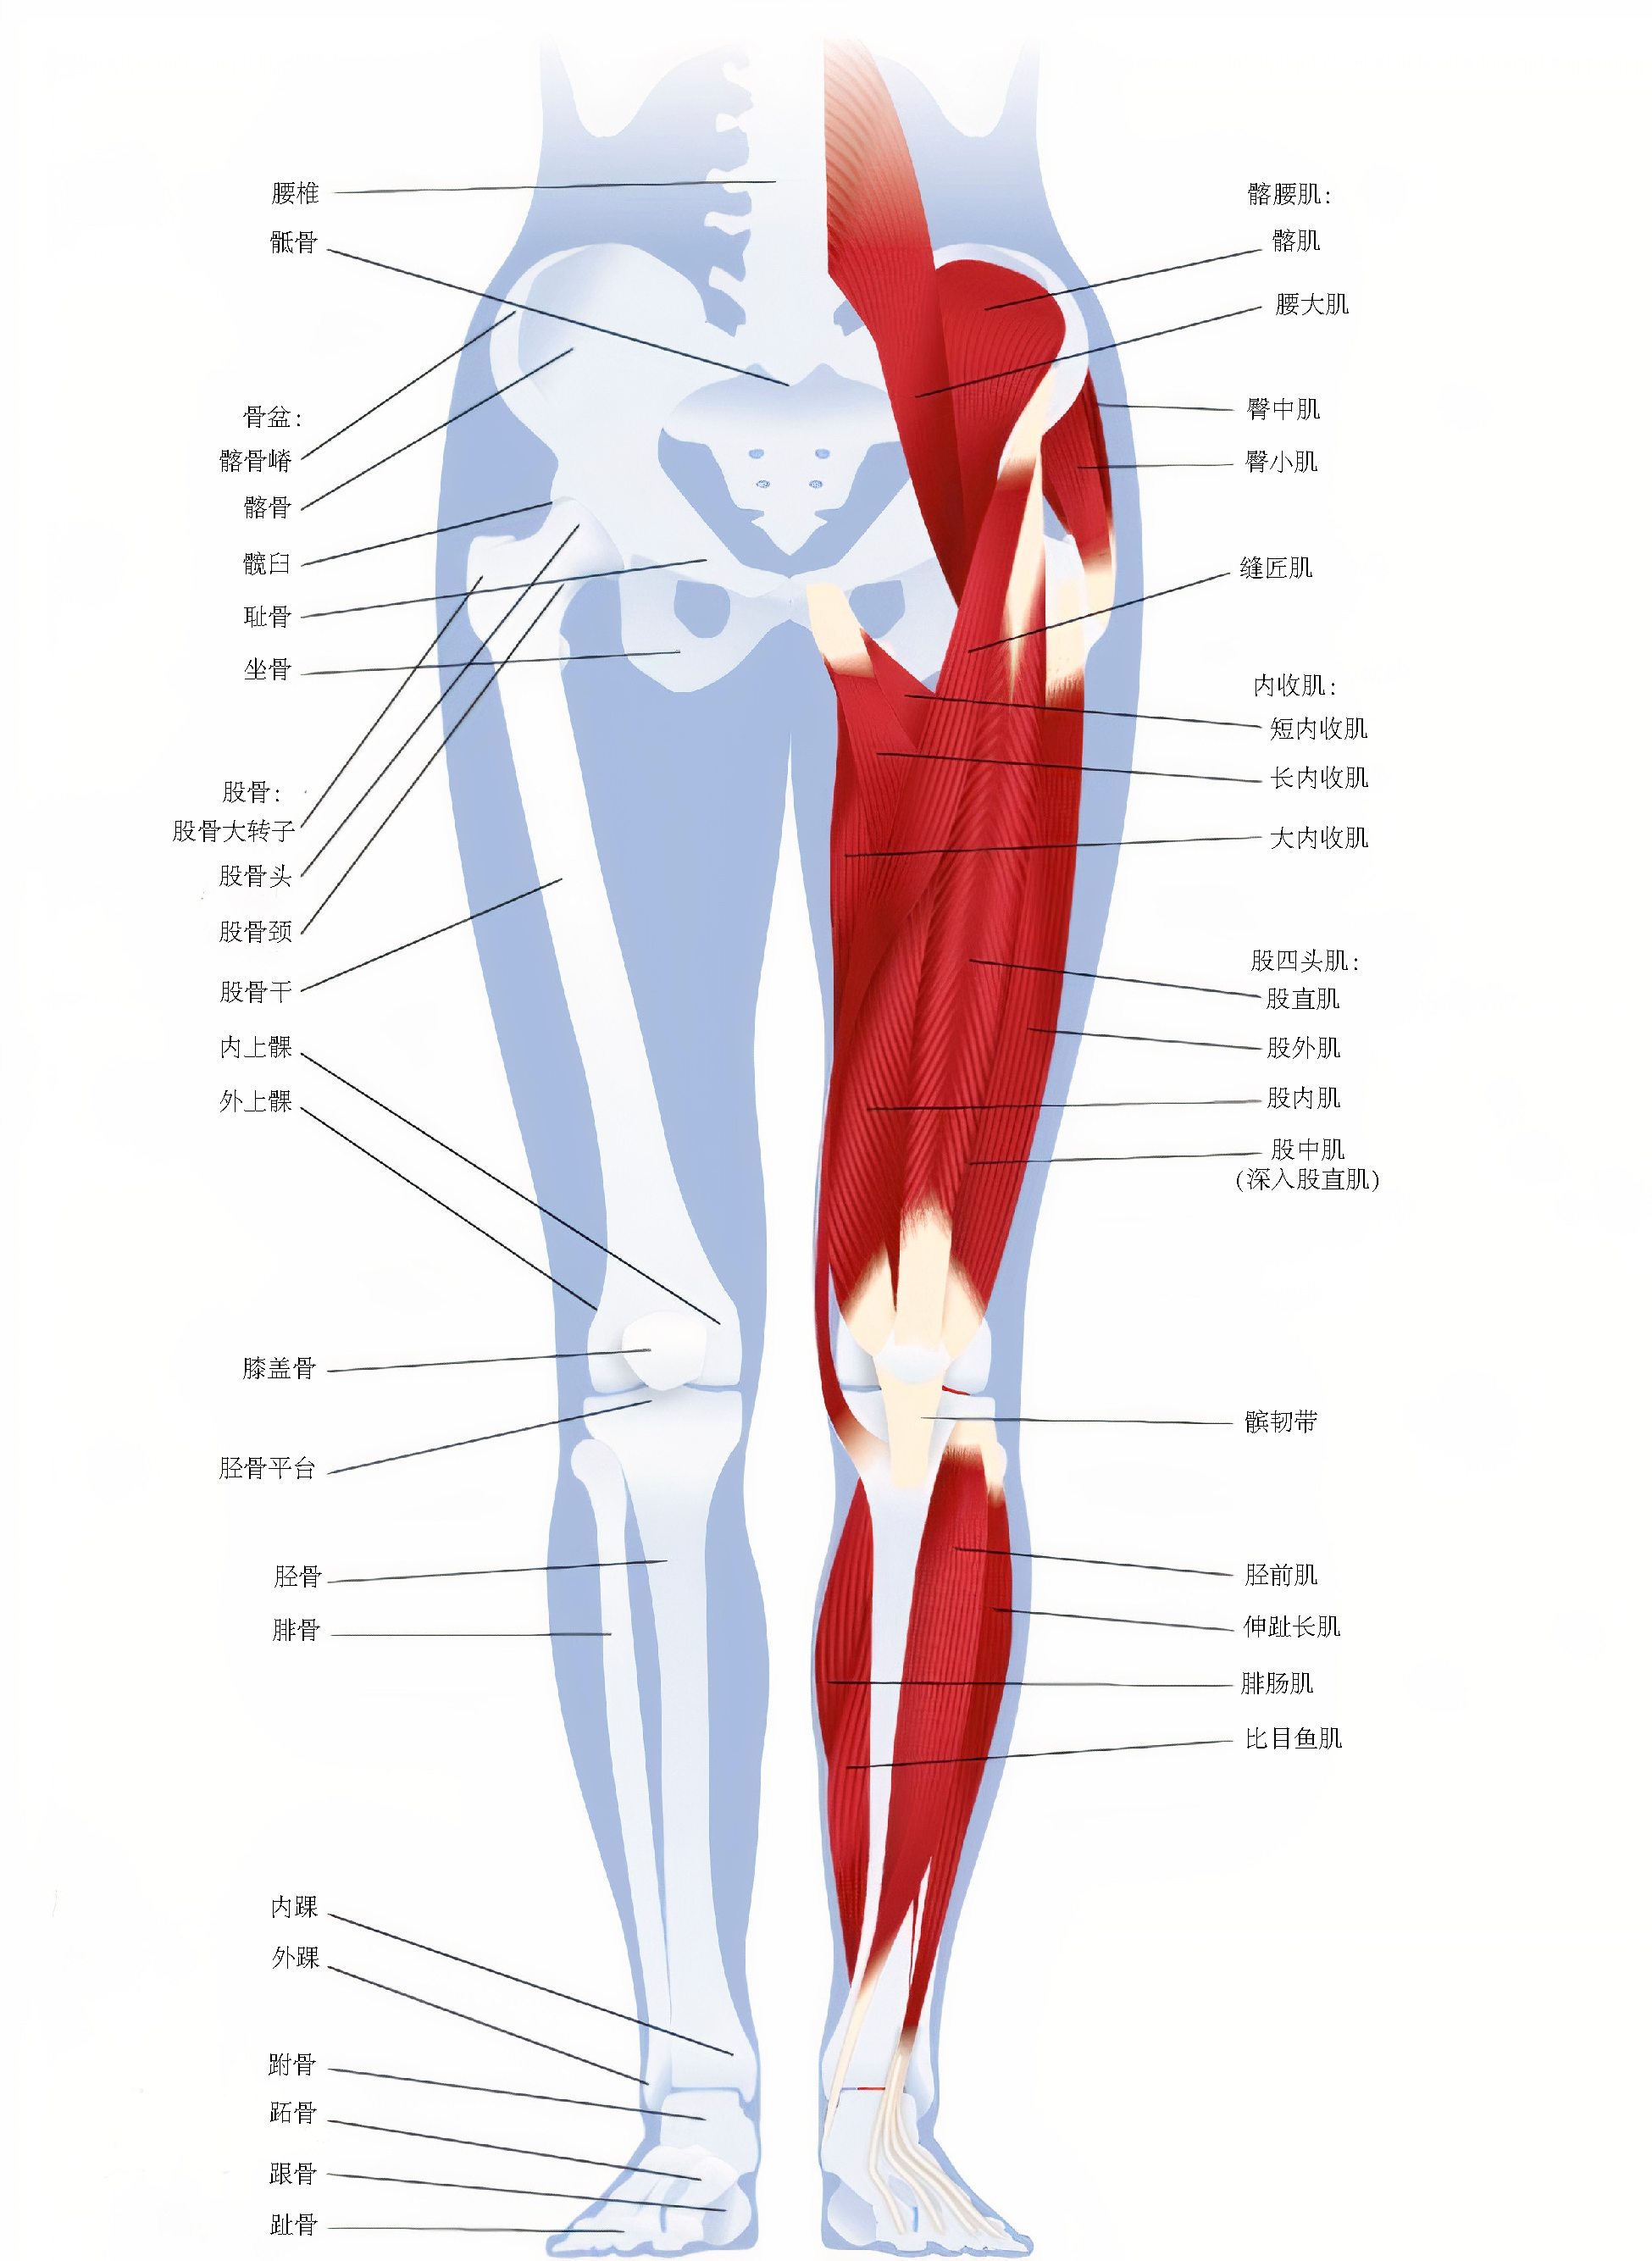
\includegraphics[width=0.95\linewidth]{chap1/1_18}
	\caption{人体下肢的主要骨骼、解剖标志和肌肉(前视图)。 \label{fig:1_18}}
\end{figure}


\begin{figure}[!htb]
	\centering
	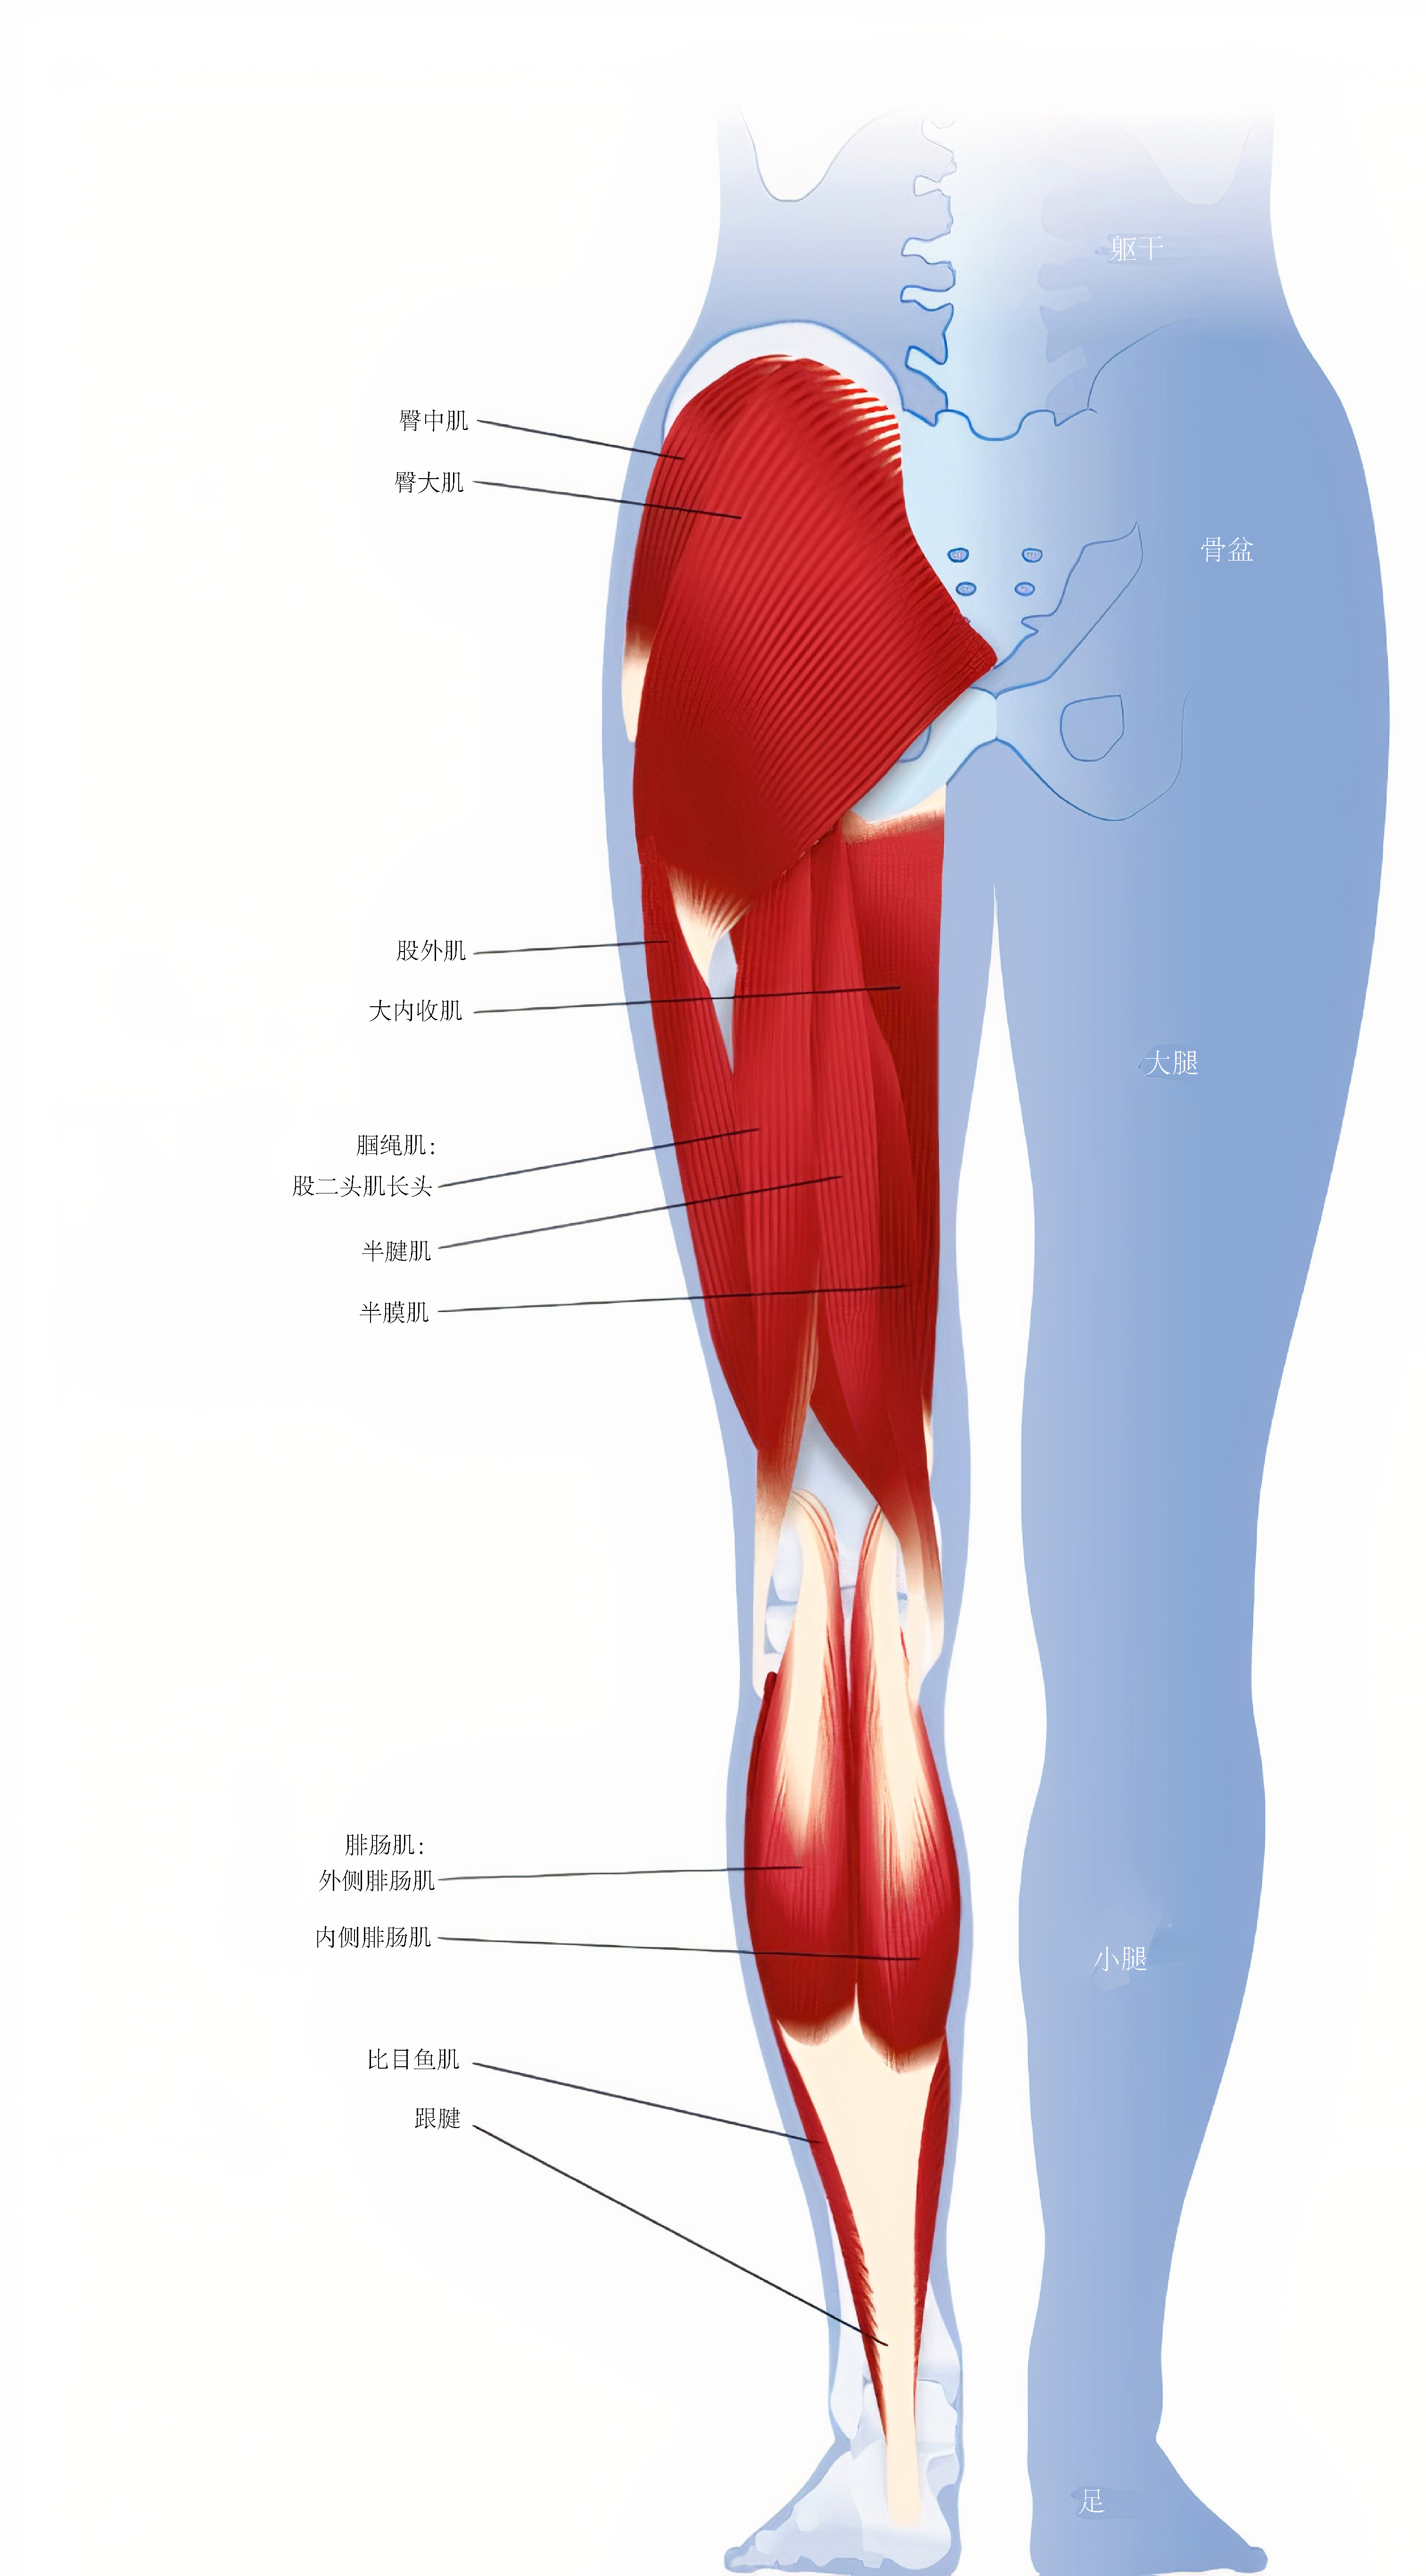
\includegraphics[width=0.75\linewidth]{chap1/1_19}
	\caption{人体下肢的身体部分和主要肌肉(后视图)。 \label{fig:1_19}}
\end{figure}


这本书只是我的一个开端,我希望它能成为你持续探索的旅程。
我们的梦想是,你能在此汇集的素材基础上,迸发出你独特的创造力火花,探索自然,创造一些能够丰富他人生活的东西。

















\chapter{行走} \label{chap:chap2}

每走一步,你都会向前倾斜一点点,然后站稳,避免摔倒,一遍又一遍,你都在摔倒,然后站稳,避免摔倒。

\begin{flushright}
	——劳里·安德森 \\
\end{flushright}

\section{概述}
前额叶皮层的进化经历了不同的阶段。
早期哺乳动物经历了一次进化,形成了所有哺乳动物共有的前额叶皮层颗粒状前额区域。
这些区域的出现能根据预测结果改善行动(第~\ref{chap:chap3}~章)和对象(第~\ref{chap:chap4}~章)之间的觅食选择。
早期灵长类动物经历了另一个进化,形成了第一个颗粒状的前额叶皮层。
原本这些动物的仅在夜间生活于细小的树枝上,它们在那里寻找、选择和获取食物,以一种需要头部和一只手协调运作的方式进食。
他们进化后的前额叶皮层有助于根据当前的生物需求和特定的习惯(第~\ref{chap:chap4}~章)来选择食物,以及在杂乱的环境中保持对食物的注意力(第~\ref{chap:chap5}~章)。
后来,在类人猿灵长类动物的进化过程中,随着这些物种及其大脑体积的增加,出现了额外的颗粒状前额叶皮层。
它们依靠最新进化的灵长类中央凹和改进的色觉在白天觅食。
因此,可以比它们的祖先更好地处理时空事件的顺序(第~\ref{chap:chap6}~章)并对资源的迹象进行检测(第~\ref{chap:chap7}~章)。
因为丰富的资源分散在类人猿的园区范围内,它们面临着严峻的资源波动、捕食和竞争问题。
他们的新前额叶皮层使他们能够通过使用单一事件来选择觅食目标(第~\ref{chap:chap8}~章)来减少风险和非生产性觅食选择的数量。




\section{介绍}

本章探讨了颗粒状前额叶皮层在早期灵长类动物中首次出现的结果,以及这种皮层仅存在于灵长类动物的情况\cite{preuss2007evolutionary}。


鉴于其名称,一些神经科学家认为颗粒状前额叶皮层的进化历史可能与生物细胞结构密切相关。
考虑到这一主张的重要性,有人可能会争辩说这是一个薄弱的支撑。
幸运的是,许多其他特征支持了“颗粒状前额叶皮层在灵长类动物中的进化”这一观点。
接下来,我们将列出其中的 4 个特征:
皮层区域之间的空间布局、颗粒状前额叶皮层向纹状体的投射模式、感觉输入的分布、以及通过电刺激皮层引起的自主神经响应。





\begin{figure}[!htb]
	\centering
	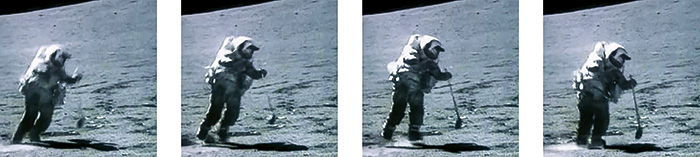
\includegraphics[width=0.9\linewidth]{chap2/2_1}
	\caption{(A)人类前额叶皮层的内侧(上)和眶上区(下)\cite{ongur2003architectonic}。 
		(B)猕猴前额叶皮层的内侧(上)和眶上区(下)\cite{carmichael1994architectonic}。 
		(C)老鼠前额叶皮层的内侧(上)和侧面(下)
		(Palomero-Gallagher\&Zilles,2004)。
		在所有图中,向左为前端。
		上行:所有图中背面向上。
		下行:(A)和(B)中,侧面向上;
		在(C)中,背面向上。
		不按比例。
		缩写:AC,前扣带皮层;
		AON,前嗅“核”;
		cc,胼胝体;
		Fr2,第二额区;
		la,不含颗粒的岛叶皮层;
		ig,灰脑层;
		IL,下极叶皮层;
		LO,外侧眶上皮层;
		MO,内侧眶上皮层;
		OB,嗅球;
		Pir,锥体(嗅觉)皮层;
		PL,前扣带区;
		tt,盖带;
		VO,腹侧眶上皮层。
		区域细分标记为尾部(c);下(i);侧面(l),内侧(m);眶上(o),后部或极端(p),前端(r),或按任意标记(a,b)。
		(A)改编自Ongur D. Ferry AT,Price JL。《人类眶上和内侧前额叶皮层的建筑分区》,《比较神经解剖学杂志》460:425-49,2003,经John Wiley和Sons许可使用。 
		(B)改编自Carmichael ST,Price JL.《猕猴颅内和眶上前额叶皮层的建筑分区》,《比较神经解剖学杂志》346:366-402,1994,经John Wiley和Sons许可使用。 
		(C)改编自Palomero-Gallagher N,Zilles K.《老鼠神经系统》中的异皮层.ed.G Paxinos,pp.729-57.圣迭戈,加利福尼亚州:爱尔斯维尔学术出版社。\label{fig:fig_2_1}}
\end{figure}


图~\ref{fig:fig_2_1}~展示了我们对人类、猕猴和老鼠这三个物种颗粒状前额叶皮层的同源性的看法,这主要归功于Preuss\cite{Preuss1991a}的开创性工作。
同源性指的是由于共同祖先的遗传而在相关物种中出现的类似区域。
该图以浅灰色显示了仅在灵长类动物中进化出来的颗粒状前额叶皮层。
这些颗粒状区域同样出现在人类和猕猴的大脑中,但不会出现在老鼠的大脑中。
老鼠只有无颗粒状前额叶皮层区域,该图为三个物种均以深灰色表示。
我们选择这三个物种,是因为我们对前额叶皮层的大部分知识都基于对它们的大脑的研究。


非颗粒状前额叶皮层区域包括下边缘皮层、前边缘皮层、无颗粒的岛叶皮层、无颗粒的眶额皮层和前扣带皮层。
在不同物种中,这些区域往往有不同的名称。
例如,啮齿动物的下肢内侧皮层与灵长类动物的25区大致相对应,von Bonin和Bailey将其称为FL区(图~\ref{fig:1_1})。


众所周知,许多神经科学家认为老鼠拥有与灵长类动物相同的前额叶皮层。
他们坚持认为,老鼠的前额叶皮层是对灵长类动物前额叶皮层的微型模拟,或者是可以将其所有属性混合在他们的小型无颗粒区域中\cite{kolb2007all,seamans2008comparing,schoenbaum2009new}。
虽然我们对此持有不同的观点,但有一个命题应该得到普遍接受:在进化历史的某个时刻,我们的某些祖先缺乏颗粒状前额叶皮层。
然而,现在我们不再缺失它。
鉴于这个历史事实,询问颗粒状前额叶皮层带来了什么优势似乎是合理的。


尽管不是每个人都同意图~\ref{fig:fig_2_1}~所描绘的同源性,但没有人严肃地质疑现代啮齿动物的大脑缺少颗粒状前额叶皮层这一事实。
对于其他哺乳动物,有一点存在争议:
有人认为狗\cite{rajkowska1988intrinsic}和猫\cite{je1948orbitofrontal}具有颗粒状前额叶皮层区域。
但当我们亲自检查组织学材料时,狗和猫所谓的颗粒状区域看起来很像猕猴和啮齿动物的无颗粒区域。


\begin{figure}[!htb]
	\centering
	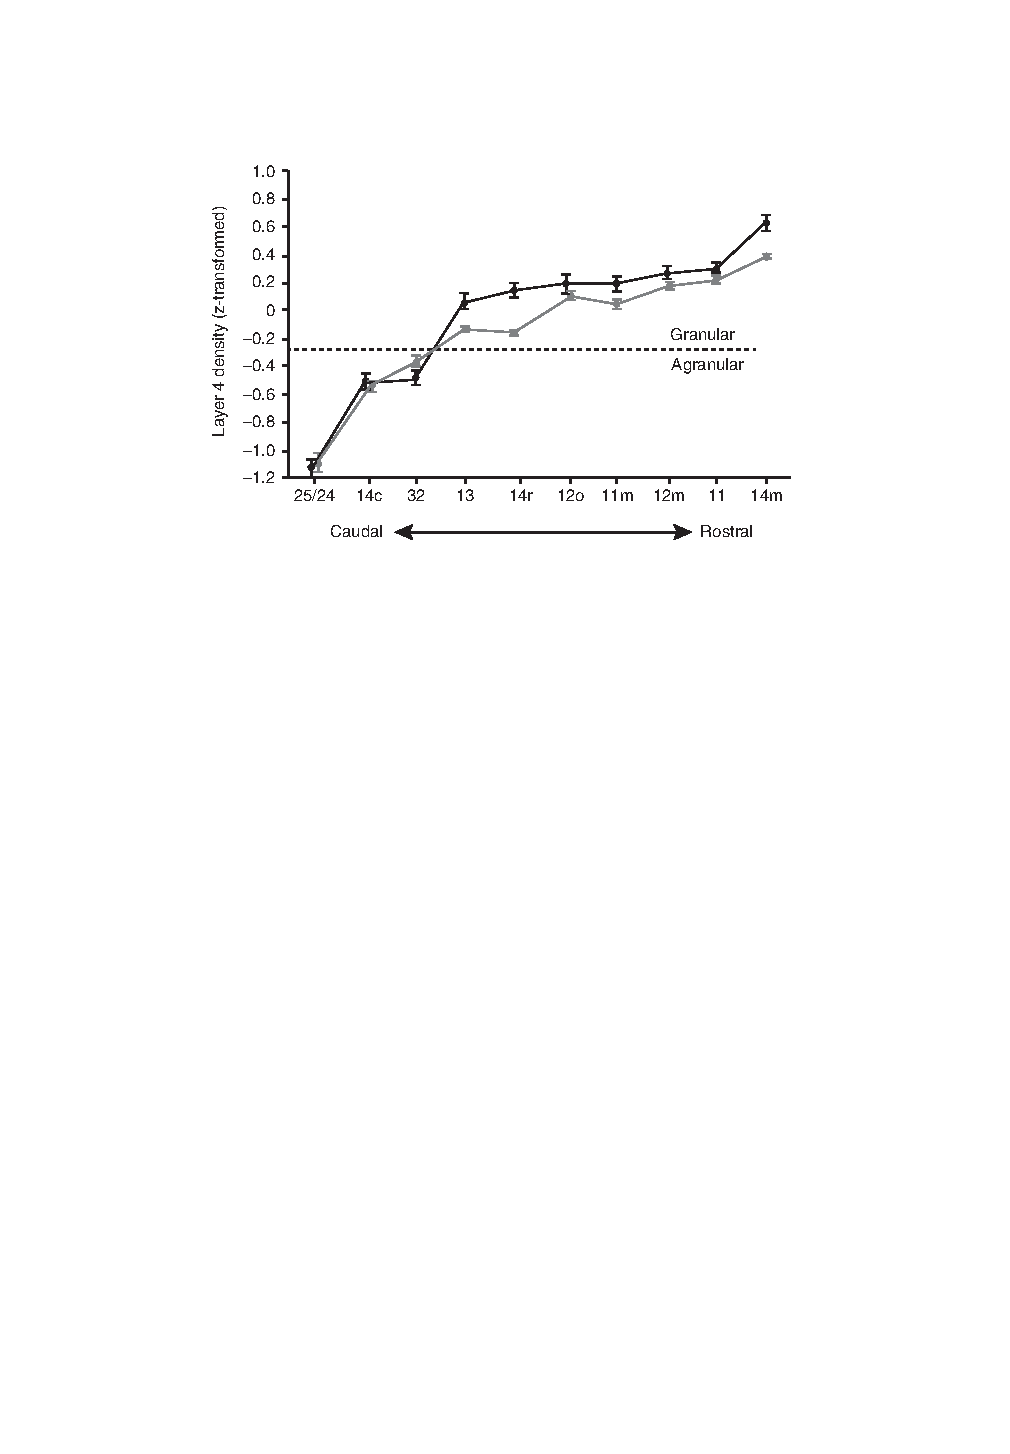
\includegraphics[width=0.8\linewidth]{chap2/2_2}
	\caption{显示了大脑额叶区域从尾向头发展的过程中,第4细胞层的归一化密度在猕猴(黑线)和人类(灰线)中的变化。
		误差条:SEM。
		该图由 Mackey S、Petrides M. 在《欧洲神经科学杂志》2010年32期(1940-1950页)中发表,经John Wiley 和 Sons出版社许可后再版。
		该图表明人类和猕猴大脑的腹内侧和侧壁眶前额叶皮层中具有可比较的成系统的区域。\label{fig:fig_2_2}}
\end{figure}


正如第~\ref{chap:chap1}~章所述,这种争议可能是由于观察者缺乏完备体系的知识方法所致。
当在猕猴和人脑中观察到这个问题时\cite{mackey2010quantitative},发现一些传统上被归类为无颗粒额叶区域的区域实际上在第 4 层细胞体密度上,与最尾端的区域相比有略微的增加。
也就是说,这些区域具有较弱的非颗粒质细胞结构,而不是纯粹的的无颗粒结构。
在食肉动物和其他非灵长类哺乳动物中发现颗粒状前额叶皮层的报告,反映了这种属性。
神经解剖学家们都认为,细胞从额叶轨道和内侧表面向头部移动时,第4层的厚度会持续增加。
因此,无颗粒皮层是否在第4层完全消失并不重要。
我们可以将第4层密度低于给定阈值的区域视为足够无颗粒这一标准,用于我们之后的研究中(如图~\ref{fig:fig_2_2}~所示)。


尽管老鼠缺乏细颗粒前额叶皮层,但一些神经科学家仍认为,老鼠前额叶皮层的中部与灵长类动物的中侧颗粒前额叶皮层(区域46)同源\cite{kolb2007all},尽管后者的是一个颗粒区域(也称为背外侧或周主前额叶皮层)。
同样,还有一些人认为,老鼠前额叶皮层的侧部与灵长类动物的整个眶前颞皮层同源,包括其颗粒部分\cite{kolb2007all,schoenbaum2009new}。
该论点基于解剖学、生理学和神经化学的相似性以及基于声称在老鼠和猕猴中的损伤效应的相似性。


然而,人们不能仅仅依据常被引用的相似性就推断其同源性。
正如 Preuss\cite{preuss1995rats}所解释的那样,人们需要对特征进行诊断,即区分一组皮层区域和其他区域的特征。
就像老鼠的非颗粒状前额叶皮层与猕猴的颗粒状前额叶皮层区域具有许多相似之处,例如编码估值的细胞。
但是,这 3 个区域——老鼠的非颗粒状前额叶皮层以及猕猴的非颗粒状和颗粒状前额叶皮层——都具有与上述细胞同样的特性,其他皮层区域也是如此。
因此,它们无法帮助我们理解前额叶皮层的进化或建立其区域之间的同源性。
例如,老鼠的非颗粒状区域的特性与灵长类动物的颗粒状前额叶皮层相似,但它们也与灵长类动物的非颗粒状前额叶皮层相似,那么这些特性就与动物的同源性无关。


有人声称,颗粒质前额叶皮层与丘脑中背核(MD)的联系是其诊断性特征\cite{je1948orbitofrontal,akert1964comparative,uylings2003rats}。
但是,MD核向实际上覆盖了额叶的几乎所有区域,包括颗粒质和非颗粒质区域。
因此,与MD核的连接不能作为诊断性特征,故它们对于同源性的问题几乎没有影响或很少有影响。


曾经有一段时间,人们认为多巴胺能输入是颗粒状前额叶皮层的特征\cite{divac1978converging,porrino1982brainstem}。
但是这些输入也终止于前额叶皮层的非颗粒状部分和运动前区,以及额叶以外大部分皮层。
事实上,在灵长类动物中,多巴胺输入到前运动皮层和后枕叶皮层的强度比大多数颗粒状前额叶皮层都要强\cite{gaspar1992topography,williams1998widespread}。
因此,多巴胺输入不能帮助我们跨物种识别前额叶皮层。


最终,损伤结果得到了进一步的研究,例如对于延迟响应任务的研究结果。
老鼠的前额内皮层损伤会导致该任务的障碍\cite{kolb1974double},类似地,猕猴颗粒质前额叶皮层的损伤也会导致该任务的障碍\cite{goldman1971analysis}。
但是,前扣带回皮层的损伤也会导致猕猴在该任务上出现障碍\cite{meunier1997effects}。
因此,该特征并非是诊断性的。
我们将在第 \ref{chap:chap10} 章中更详细地讨论这个问题,老鼠和猕猴所出现的的障碍虽然在表面上相似,但在重要的方面存在差异。


值得注意的是,我们并不是说灵长类动物拥有前额叶皮层而其他哺乳动物没有。
我们认为非灵长类哺乳动物也有一些可以合理称之为前额叶皮层的区域。
第~\ref{chap:chap3}~章和第~\ref{chap:chap4}~章将这些非颗粒质区域纳入了内侧和眶前颞皮层。
但我们不赞同非灵长类哺乳动物具有类似于灵长类前额叶皮层的微型复制品或混合体的观点。
非灵长类哺乳动物缺乏灵长类动物的颗粒质前额叶皮层以及执行其基本功能的任何区域。
因为忽略了这些概念,文献中存在很多将非同源区域的结果混合在一起的实例,例如,引用灵长类动物的中侧前额叶皮层(46区)的研究结果来支持与啮齿动物的前额内皮层相关的某些结论。但其实这不是最好的方式。


我们对同源性的结论不应该引起太多争议。
以视觉皮层为例,所有灵长类动物都共享10-20个视觉区域,其中有些物种甚至拥有更多的视觉区域\cite{kaas2020evolution}。
举个例子,一个被称为MT或V5的区域在视网膜中央凹有精细的专门分化功能,用于分析视觉运动。
但老鼠的视觉区域少得多\cite{rosa1999evolution,lyon200734},不可能复制灵长类动物10-20个视觉区域的所有功能,并且它们缺乏中央凹。
另外,在缺乏中央凹的物种中进行视网膜中央凹的微观分析是不太可能的。


再以另一个例子为例,考虑到蝙蝠听觉皮层的回声定位功能。
这些动物使用类似声纳的系统来检测它们与猎物的距离和猎物本身的速度。
蝙蝠的听觉皮层有许多专门区域来处理与回声定位相关的声学信号,包括分析调频声音、多普勒频移等\cite{suga1997cortical,fitzpatrick1998distribution}。
但如果老鼠的听觉皮层中的一些细胞也对类似的声音作出响应,这并不意味着它们执行与蝙蝠听觉细胞相同的功能。
事实上,想象老鼠使用回声定位来追踪它们的食物是很奇怪的。
同样,认为老鼠的少数听觉区域具有与回声定位蝙蝠的大量专门区域相同的所有功能和属性是缺乏可信度的。


很少有神经科学家质疑这样的观点:与老鼠共同祖先相比,声呐定位蝙蝠拥有新的听觉区域,而灵长类动物拥有新的视觉区域,以适应其在视觉敏锐度和色彩视觉方面的需求。
同时,这些新区域支持新的功能,如对凹视动作或回声定位的分析,这一观点已经被广泛接受。
因此,令人惊讶的是,同样的神经科学家们往往对这样一个想法犹豫不决:灵长类动物拥有新的前额区域,并且这些区域具有新的功能。


问题的一部分来自于使用“新”的词来描述区域或功能。
有人提出,新的区域通过复制和随后的分化出现\cite{krubitzer2000arealization}。
如果是这样的话,那么合理的假设是,某些新区域的分化程度比其他区域低;
当它们在许多哺乳动物中出现时,我们可以将更保守的区域识别为同源的。
然而,在这样做时,我们需要认识到大多数进化所产生的变化都涉及到同源结构的修改,因此在物种之间具有绝对等价是不现实的。


相较于这些相对保守的区域,其他的复制产物则更加具有差异化,因此应该被称为新的区域。
随着差异化的产生,它们开始执行新的功能,从而提供了优于其祖先状态的优势。
然而,当这些新区域进化时,它们会与附近的区域共享属性,并且通常会与它们有轴突连接。
因此,虽然前额叶皮层的颗粒层和无颗粒层部分具有许多共同特征。
但是我们不应该基于此得出它们是同源或类似的结论。
颗粒状的前额叶皮层专门在灵长类动物中进化而来,并发展为支持灵长类动物具有特别能力的区域。


\section{原猴亚目前额叶皮层}

灵长类动物前额叶皮层进化的最有力证据来自对原猴亚目的研究。
鉴于这一证据的重要性,我们将对其详细审查。
此外,读者可以从本节末尾的摘要中了解该论点的要点。


\begin{table}[htbp]
	\newcommand{\tabincell}[2]{\begin{tabular}{@{}#1@{}}#2\end{tabular}} %换行指令
	\centering
	\caption{本章中使用的生物学术语}
	\renewcommand\arraystretch{1.5}	%设置表格内行间距
	\begin{tabular}{ll}
		\toprule
		术语 & 含义 \\
		\midrule
		进化 & 与祖先状态不同,具有差异化的  \\
		埃及古猿 & 一种已灭绝的类人猿,接近早期的狭鼻类动物  \\
		类人猿 & 猕猴、猿类和人类  \\
		食果猴 & 一个已经灭绝的古老哺乳动物类群  \\
		智利猴 & 一个灭绝的类人猿,接近于最早的阔鼻猴  \\
		狭鼻猿& 旧大陆灵长类动物(旧大陆猴、类人猿和人类),从阔鼻猿中分化出来  \\
		类人猿亚目& 眼镜猴与类人猿;从原猴类中分化出来  \\
		同源性& 从共同祖先继承而来的相似性,与由平行或趋同进化引起的相似性形成对比  \\
		旧大陆猴& \tabincell{c}{一组狭鼻猴类灵长目动物,包括猕猴、狒狒、长尾黑颚猴(绿猴)、\\白眉猴、长尾猴、山魈猴和红尾猴}  \\
		%内容换行
		副猿& 已灭绝的类人猿,接近于第一个类人猿,也被称为Simonsius  \\
		阔鼻猴& 新大陆猴,包括鬃狮猴、松鼠猴、枭猴和卷尾猴;从狭鼻猿中分化出来  \\
		更猴形类群& 已经灭绝的哺乳动物,可能是早期灵长类或早期灵长类的近亲,包括食果猴  \\
		原始的& 类似于祖先的情况  \\
		原猴亚目& 原猴类灵长类动物和猴鼠目动物; 不构成一个天然类群  \\
		原猴类& 大多数原猴类灵长类动物,包括狐猴、懒猴和丛林婴猴;从类人猿中分化出来  \\
		\bottomrule
		\label{tab:tab_2_1}
	\end{tabular}%
\end{table}%


讨论中必要地使用了一些可能不是所有神经科学家都熟悉的术语,因此表~\ref{tab:tab_2_1}~列出了这些术语以便参考。
主要的灵长类动物群组包括原猴亚目、原猴类、类人猿亚目和类人猿。
在进化过程中,灵长类动物分裂成原猴类(湿鼻)(lemurs, lorises), 和丛林婴猴,构成了大多数称为原猴亚目的灵长类动物和类人猿亚目(干鼻)(包括狐猴,人猿和类人猿)。
类人猿亚目包括所有新大陆猴(Platyrrhines),以及旧大陆猴、大猩猩和人类(统称为狭鼻猿)。


接下来,我们假设现代灵长类动物和类人猿共有的特征可能存在于它们最后的共同祖先身上。
由于那个祖先是早期的灵长类动物,因此我们认为这些特征也是早期灵长类动物的特征。
我们还假设类人猿具有但灵长类动物没有的特征可能是在类人猿中进化出来的。
像之前一样,在形成分支后,独立进化也在继续进行,因此灵长类动物可能具有类人猿所缺乏的适应性。


和几个其他颗粒状前额叶皮层区域一样\cite{Preuss1991a},灵长类动物的皮层缺乏中侧前额叶皮层(区域46)的同源区。
相反,他们确定了尾部前额叶皮层(区域8)和眶额皮层的颗粒状部分的同源区。
Preuss 用各种论证支持了他们的结论,其中包括比较丛林婴猴和恒河猴的共同之处\cite{preuss1991ipsilateral}。
他们还考虑了其他人在狐猴(另一种原猴类灵长类动物)上所做的工作。
然而,他们大部分证据来自于对丛林婴猴和恒河猴前额叶皮层结构的研究。
最近,一项研究证实了他们所分析的大部分内容\cite{wong2010architectonic}。


\subsection{皮层结构}

\begin{figure}[!htb]
	\centering
	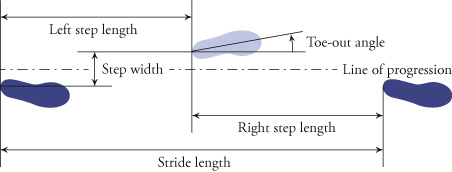
\includegraphics[width=0.8\linewidth]{chap2/2_3}
	\caption{灵长类动物额叶皮层的建构图。
		所有图中,前端朝左。
		从上到下依次为背侧视图:向内为上;
		外侧视图:背侧向上;
		内侧面视图:背侧向上;
		腹侧面视图:侧面向上。
		缩略语如图 \ref{fig:fig_2_1} 所示,包括以下内容:Gr,颗粒区,分为前部(A),背部(D),侧部(L),中部(M),后部(P);PrCO/OFO,前中央卷叶区/眶前额叶卷叶区;6ds,背区域6的沟部分;FPC,额极回扣带区;MF,中央前额叶皮层;VL,腹侧区域。
		摘自Preuss TM,Goldman-Rakic PS。灵长类动物狨和人猿类动物猕猴的颗粒前额叶皮层及其周围区域的髓样和细胞样结构。《比较神经学杂志》310:429-74  1991,John Wiley and Sons,获准使用。\label{fig:fig_2_3}}
\end{figure}


图~\ref{fig:fig_2_3}~显示了Preuss和Goldman-Rakic为丛林婴猴额叶皮层绘制的图。
在本节中,我们将对其进行详细的介绍与分析,以供对解剖学细节感兴趣的读者参考。


首先,Preuss和Goldman-Rakic确定了运动前皮层的不含颗粒的区域(区域6)。
在紧贴区域6的前额叶表面皮层上,包括一个独特的区域,具有“非常厚、密”的第4层和髓鞘化的纤维束,这些纤维束从皮层下白质向第4层延伸,在那里分散到更浅的层中。


Preuss和Goldman-Rakic得出结论,这个被称为后颗粒区(GrP)的区域(图~\ref{fig:fig_2_3})与猕猴和人类的8区同源。
在该区域进行电刺激会引发灵长类动物\cite{wu2000converging}和猕猴\cite{bruce1985primate}的眼动作,这一发现支持了GrP区域包括额叶视区的结论。


Preuss和Goldman-Rakic指出,区域GrP在内侧被后-中颗粒区(GrPM)包围,在外侧被后-侧颗粒区(GrPL)包围(见图~\ref{fig:fig_2_3})。
他们认为GrPM和GrPL分别对应于8Ad区和45区的一部分。
这个结论并不仅仅是基于它们与GrP和6区的拓扑关系。
Preuss和Goldman-Rakic还指出,在灵长类动物和恒河猴的内侧和外侧区域中,锥形细胞比GrP区域小,横向定向的髓鞘束比GrP区域更显著。
根据类似的基础,他们得出结论,更内侧的区域称为背颗粒皮层(GrD)和内侧颗粒皮层(GrM)(见图~\ref{fig:fig_2_3}),分别与恒河猴的8B区的背部和内侧部分同源。


Preuss和Goldman-Rakic谨慎地指出,他们推测灵长类动物的颗粒质前额叶皮层更向前部位的同源区,例如前背侧颗粒区(GrAD)。
他们还考虑了两种可能性:一种是灵长类动物的GrAD与猕猴和人类的区域8Ad的前部同源。
这个想法基于GrP仅与猕猴的区域8Ad的尾部同源,留下其前部“自由区域”成为GrAD的同源区。
另一种可能性是,GrP可能是猕猴的区域8Ad的前部和尾部的组合同源区。
在这种解释下,区域GrAD可能与猕猴大脑中的后外侧前额叶皮层(区域9/46)同源,或者由于其与后顶叶皮层之间的联系不强,与额极皮层同源\cite{preuss2007evolutionary}。
这个问题还没有解决,但重要的是,Preuss和Goldman-Rakic没有发现GrAD与中侧前额叶皮层(区域46)对应的证据,这个结论受到了区域GrAD与后顶叶皮层之间连接较弱的支持。


至于眶额皮层,Preuss和Goldman-Rakic建议,灵长类动物的腹侧颗粒区(GrV)可能对应于猕猴的11区(参见图~\ref{fig:fig_1_2})。
并且,总体而言,他们得出结论是灵长类动物具有与猕猴差不多数量的眶部亚区。


Preuss和Goldman-Rakic无法确定类似于GrAL的区域在狨猴脑中的同源区,因此他们认为这个区域是在类狨目和类灵猴目分化后在狨猴中演化出来的。


作为他们最重要的观点之一,Preuss和Goldman-Rakic指出,许多猕猴大部分前额叶皮层的髓鞘比额叶皮层的要少,而且在灵长类动物的额叶皮层中似乎不存在这样的髓鞘较少的区域。
一项最近的结构成像研究将这个论点扩展到黑猩猩和人类中\cite{glasser2011comparative}。
除了一些基于连接性的论证之外,他们得出了这样的结论:除非灵长类动物中的灰瘤质区域与其他动物有所不同,否则包括9、12/47和46区域以及可能的10区域在内的这些髓鞘较少区域在灵长类动物演化中是在单鼻亚目分化后进化出来的,而现代的猕猴、大猩猩和人类通过继承拥有了它们。
刚才提到的所有区域都具有灰质细胞形态学和少量的髓鞘,并且它们构成了现代人猿类,包括人类的大部分前额叶皮层。


\subsection{拓扑结构}

拓扑学术语指的是大脑皮层结构的空间排列方式,具体指皮层区域在二维皮层平面内的相对位置,可以想象将其展开以显示脑沟和脑回。
例如,Preuss和Goldman-Rakic使用GrP与运动前皮层 (区域6)之间的拓扑关系来确定它是短尾猴额叶视区的同源物。
拓扑学术语在皮层进化的出版讨论中很少使用,但空间结构之间的证据一直是评估同源性最重要的特征之一。
通常情况下,邻近结构为解释某些原本难以理解的结构提供了重要的指导,这是因为身体的基本模式在进化发育中是比较保守的特征之一。


前额叶皮层拓扑结构中一个特别重要的方面涉及其与异皮层的关系。
如图~\ref{fig:fig_2_1}~所示,一些前额区域直接相邻于黑色所示的异皮层。
与大多数大脑皮层相比,异皮层仅有 3 个层次,其层次结构相对简单。
典型的例子包括海马体和嗅叶皮层。


前额叶皮层的非颗粒部分靠近分配性皮层。
例如,在啮齿类动物和灵长类动物中,无颗粒岛叶皮层毗邻嗅叶皮层和前嗅核。
尽管前嗅核被称为“核”,但它是一种分配性皮层结构。
其他非颗粒额叶区域,如前扣带皮层、下肢内侧皮层和前肢内侧皮层,毗邻更小、更不为人知的分配性皮层区域。
虽然一些权威机构已经为靠近分配性皮层的皮层区域开发了复杂的名称,例如近分配皮层或前额叶皮层,但我们主要是基于比较的原因将它们全部视为新皮层的变体。


因此,非颗粒状前额叶皮层区域不仅可以通过其细胞结构进行识别,还可以通过它们与非皮层相邻来识别。
相比之下,颗粒状前额叶皮层区域不与非皮层相邻,而是靠近非颗粒状前额叶皮层区域。
因此,拓扑学和细胞结构都认为颗粒状前额叶皮层区域与非颗粒状前额叶皮层区域不同。
需要注意的是,这种分析不包括运动皮层和前运动区,尽管它们也是非颗粒状的。


\subsection{皮层投射}

我们的论点也得到了某些皮层投射的支持。
例如,在啮齿动物中,通常称为眶前额叶皮层或眶额皮层的区域向纹状体发送直接投射。
仔细研究这个投射的细节提供了一些诊断特征,基于这样一个假设,即额叶皮层的同源部分向纹状体的同源部分投射。


在老鼠中,来自下肢内侧区和前扣带区的投射主要终止于伏隔核壳,这是腹侧纹状体的一部分\cite{brog1993patterns,reynolds2005specificity}。
纹状体分为两部分,腹侧纹状体包括伏隔核以及其他一些结构,而背侧纹状体包括尾状核和腹侧核。
猕猴的25区和32区也投射到伏隔核壳\cite{haber1995orbital,haber2006reward},这一特征支持它们与啮齿动物中被称为下肢内侧区和前扣带区的区域的同源性。


在猕猴中,颗粒状前额叶皮层区域根本不投射到任何地方的伏隔核,更不用说它的壳了,它们也不投射到任何其他的腹侧纹状体区域。
相反,它们投射到背侧纹状体的一部分,具体来说是尾状核\cite{selemon1985longitudinal}。
因此,从详细的皮层-纹状体终止模式得出的结论与从细胞结构和拓扑学得出的结论一致。
颗粒状前额叶皮层没有在老鼠中的同源物。


同样的规律也适用于眶额叶皮层。
在老鼠中,眶前额叶皮层投射到腹侧纹状体或其附近\cite{berendse1992topographical}。
在猕猴中,眶前额叶皮层的无颗粒部分(包括无颗粒岛叶区域)向这些纹状体部位发送大量的投射。
但是,额叶皮层颗粒质部分投射到背侧纹状体。
与半球外侧颗粒质前额叶皮层一样,额叶表面的颗粒质区域主要投射到尾状核\cite{haber1995orbital,haber2006reward,ferry2000prefrontal,ongur2000organization}。


神经解剖学家描述了灵长类动物中新的前额叶皮层区域及其皮层纹理-尾纹突出部向腹侧移位的现象,将其称为“腹侧移位”\cite{schilman2008orbital}。
在老鼠中,非颗粒层的前额叶皮层投射于纹状体的背部和腹部之间。
然而,在灵长类动物中,同源的非颗粒层的前额叶皮层的投射终止于纹状体的腹部三分之一位置。
这种腹侧移位与新的前额叶皮层区域投射到更背部的纹状体区域是一致的。


我们在这里指出的现象,与那些认为啮齿动物的背内侧纹状体与灵长类动物的尾状核是同源的人存在分歧的主要原因是基于拓扑\cite{balleine2010human}。
在啮齿动物中,内囊并没有像在灵长类动物中那样将尾状核与壳核分开。
这使得在背纹状体内进行同源性分配变得困难,这也是为什么Balleine和O'Doherty得出他们的结论的原因。
然而,他们的同源性观点几乎没有任何来自比较神经解剖学的支持。
灵长类动物的尾状核的一个小的腹部可能在啮齿动物中有同源物。
然而,尾状核的头部以及向其投射的纹状前额叶皮层区域是在灵长类动物中进化形成的。


此外,在灵长类动物中,相比于灰质前额叶皮层-上丘(superior colliculus)弱的皮层-上丘投射,灰质前额叶皮层对皮层-上丘的投射更为强烈\cite{preuss1995rats}。
然而,我们不认为这是一个主要的论点。
虽然它适用于灰质前额叶皮层的背侧、内侧、腹侧、额极和尾侧,但眶额皮层对皮层-上丘的投射并不显著\cite{leichnetz1981prefrontal}。


\subsection{感官输入}

额外的联系支持了我们的论点。
在老鼠和猕猴中,无颗粒前额叶皮层的部分相对直接地接收嗅觉、味觉和内脏输入\cite{ray1993organization},正如~\ref{chap:chap4}~章更详细地讨论的那样。
嗅觉输入来自梨状皮层;
味觉和内脏感觉输入通过脑干和丘脑中继抵达无颗粒前额叶皮层。
这些联系支持了灵长类和啮齿动物无颗粒眶额皮层的同源性。
眶额皮层的颗粒状部分缺乏这种特征,仅通过无颗粒额叶区间接地接收这些感觉输入。


\subsection{自主输出}

\begin{figure}[!htb]
	\centering
	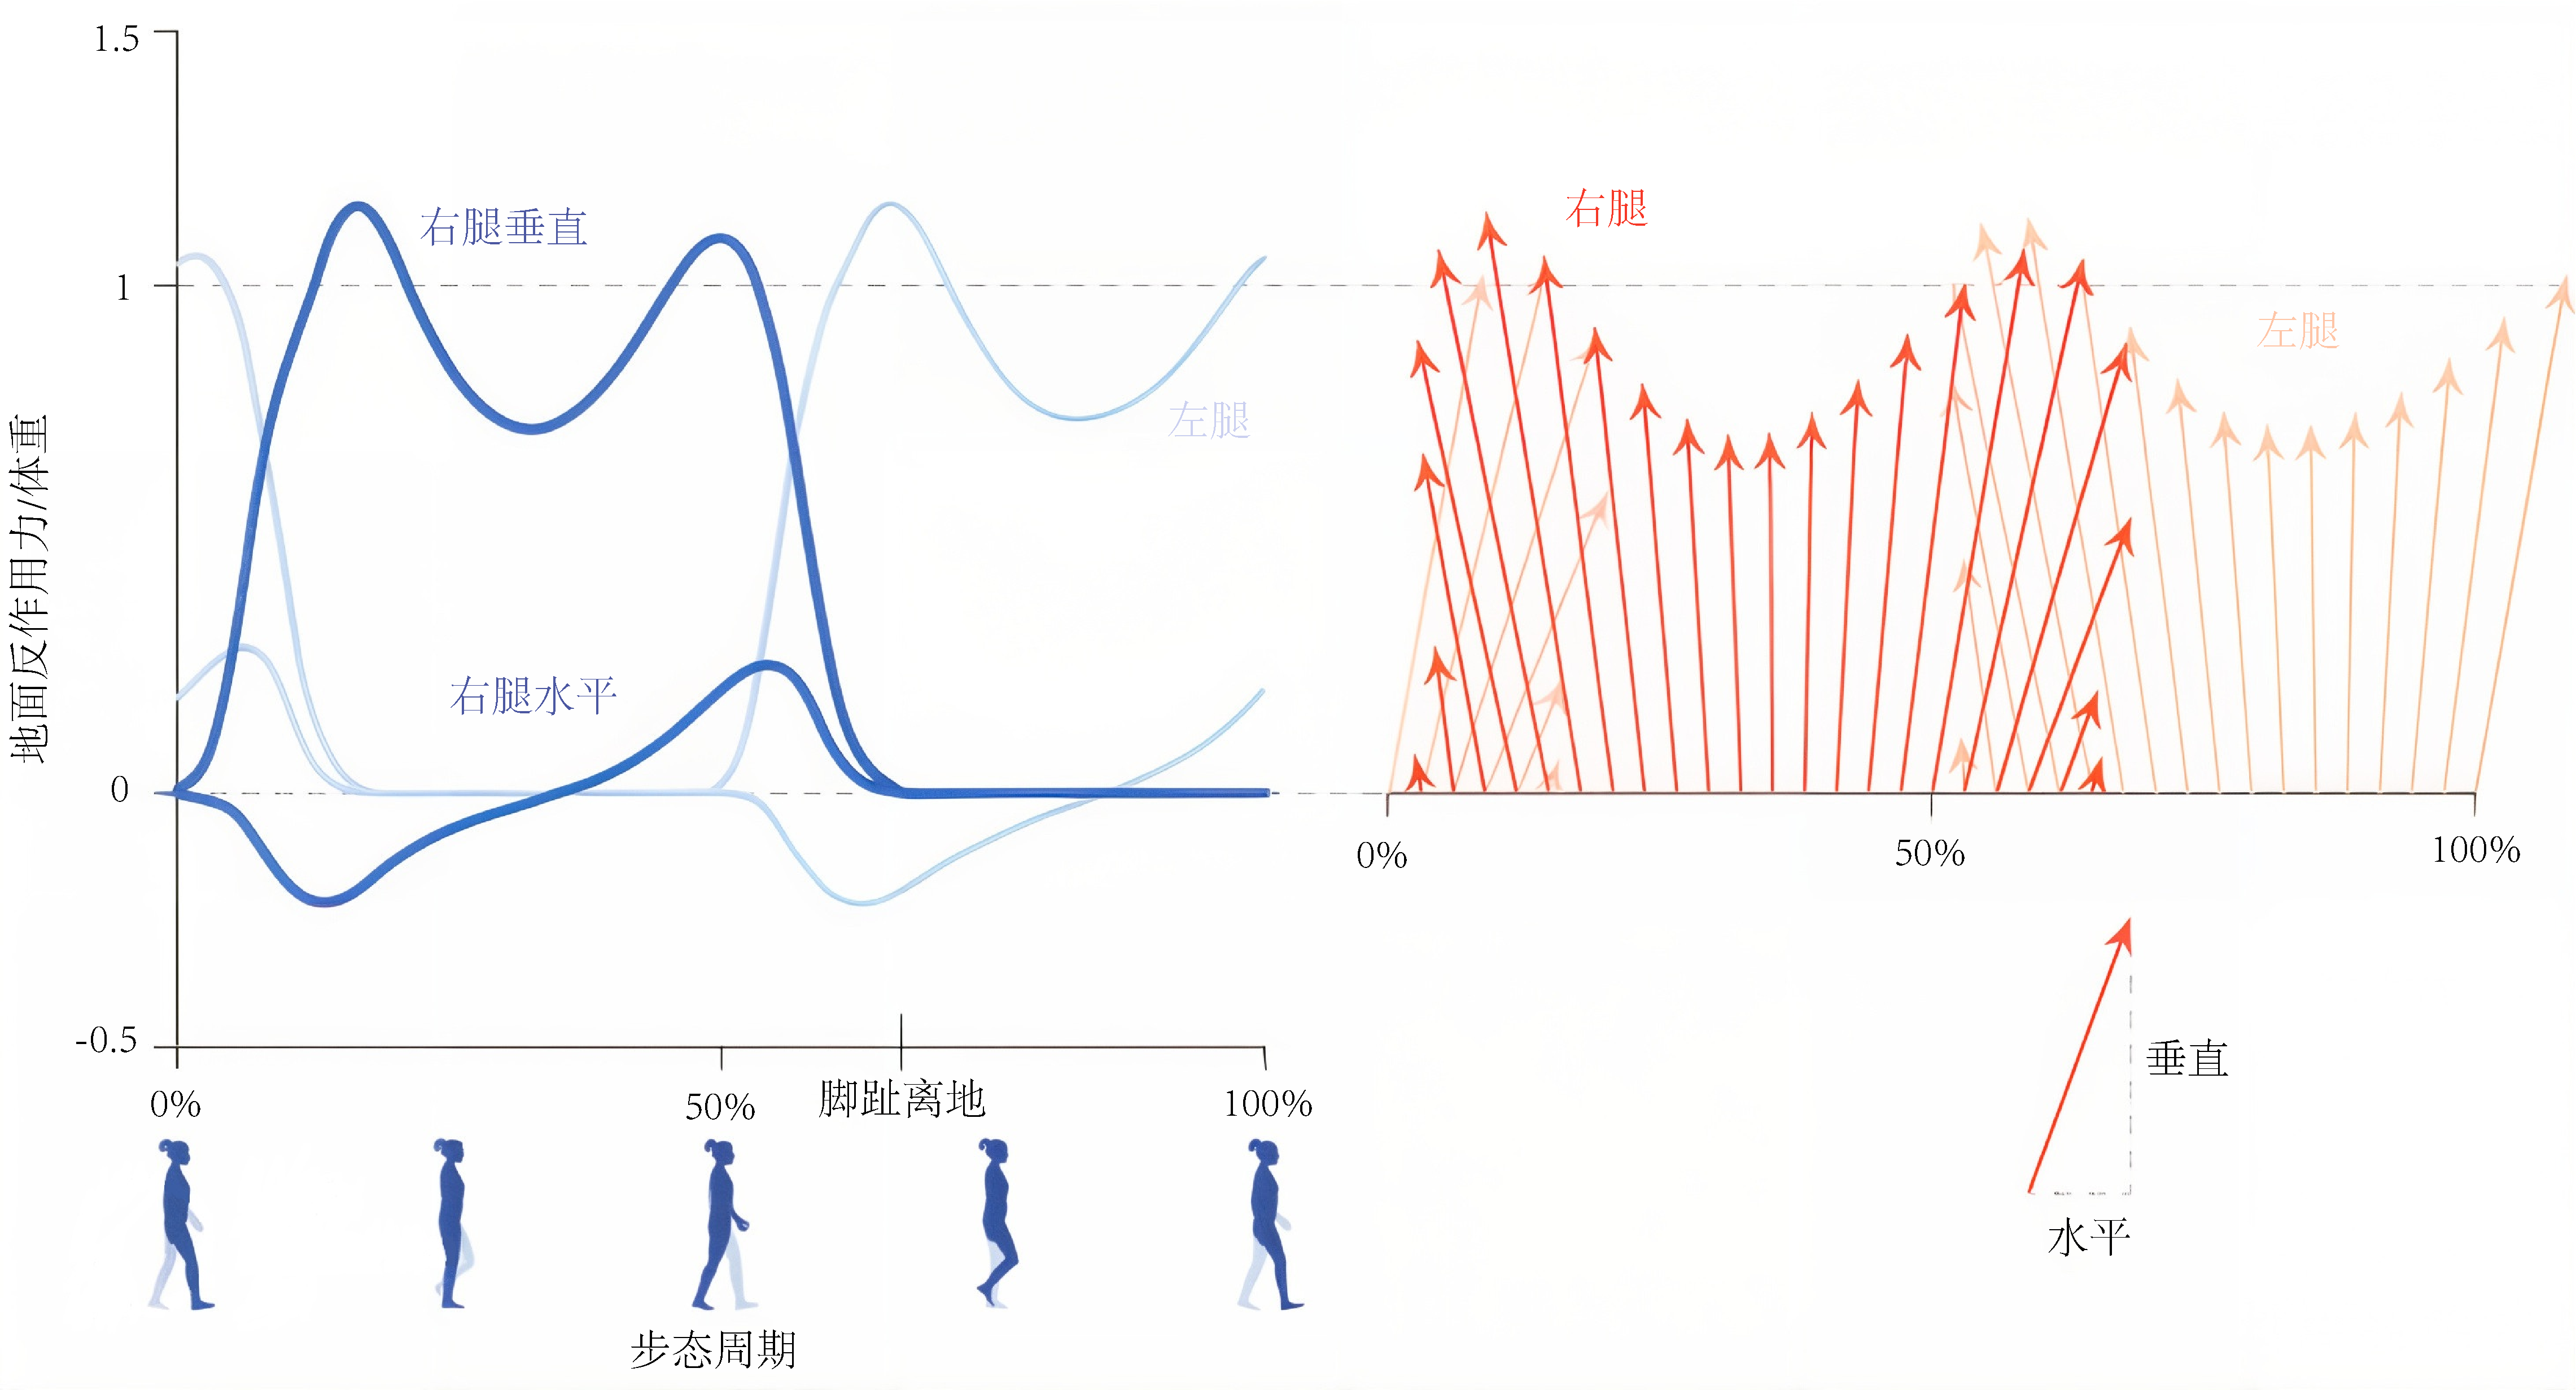
\includegraphics[width=0.9\linewidth]{chap2/2_4}
	\caption{展示了对猕猴大脑区域进行电刺激引发自主神经效应的区域(用点状线填充)。
		左图为侧面视图,右图为内侧视图。
		左图中电刺激区域包括:
		A,颗粒和非颗粒岛叶皮层(无效应);
		B,非颗粒岛叶皮层;
		C,尾侧(非颗粒)眶额皮层;
		D,颞下皮层(无效应);
		F,颞极皮层。
		右图中电刺激区域包括:
		A,前扣带皮层(见第 \ref{chap:chap3} 章);
		B,前扣带皮层;
		C,亚扣带、下肢带皮层;
		D,颞极皮层。
		注意,刺激非颗粒区域会产生自主神经效应,而刺激颗粒区域则没有\cite{kaada1949respiratory}。\label{fig:fig_2_4}}
\end{figure}


啮齿动物和灵长类的无粒质前额叶皮层与灵长类的颗粒状前额叶皮层还有其他不同之处。
来自无粒质前额叶皮层的输出比颗粒状前额叶皮层更直接地影响自主神经系统。
如图~\ref{fig:fig_2_4}~所示,电刺激猕猴的最后部分的颞上回皮层,包括无粒质岛层,以及前扣带回皮层和下肢回皮层会引起自主响应\cite{kaada1960cingulate}。
这些响应包括呼吸速率的变化、血压的变化、脉率的变化、瞳孔扩张和毛发竖立。
颗粒状前额叶皮层的刺激,包括颗粒状的部分,没有这样的响应\cite{kaada1949respiratory}。


沃克(1940年)的额叶皮层地图并没有意识到13区和14区具有颗粒和无颗粒部分,但其他人已经注意到\textit{眶额皮层}后部具有无颗粒的细胞结构\cite{carmichael1994architectonic}。
图2.1说明了14c区和13a区的这种特性\cite{mackey2010quantitative},最近通过定量细胞结构分析对此进行了确认(图~\ref{fig:fig_2_2})。
Carmichael\cite{carmichael1994architectonic}将无颗粒岛叶皮层包括在前额叶皮层的眶组中,这进一步加强了基本观点。


如果其他哺乳动物的无颗粒前额叶皮层与灵长类动物的无颗粒额叶皮层同源,那么对这些区域的电刺激应该产生自主神经效应。
正如预测的那样,这个特性已经在老鼠、兔子、猫、狗、多种猕猴和人类中得到证实。
例如,刺激内侧前额叶皮层会在兔子\cite{powell2005single}和老鼠\cite{scopinho2009medial}中引起心动过缓。
此外,兔子\cite{powell1997amygdala}和老鼠\cite{frysztak1994effect}无颗粒前额叶皮层的损伤会破坏对预测生理应激物的刺激对自主响应的调节。


\subsection{小结}

颗粒状前额叶皮层和无颗粒前额叶皮层的区别不仅由皮层细胞结构和髓鞘结构支持,还由区域之间的拓扑关系、皮层纹状体连接的模式、感觉输入和自主输出的模式支持。
因此,通过比较灵长类动物与其他哺乳动物,我们可以得出以下结论:\par

1.非灵长类哺乳动物缺乏灵长类动物颗粒状前额叶皮层的同源结构;\par

2.灵长类动物和其他哺乳动物具有几个同源的无粒状前额叶皮层区域:下肢前区、前扣带回、前扣带皮层、无粒状眶额皮层和无粒状岛叶皮层;\par

3.这些无颗粒前额叶皮层区域可能是从最早的哺乳动物所演化出来的,因为迄今为止检查过的所有哺乳动物都有这些区域的同源结构,而在非哺乳类脊椎动物中没有发现同源结构。


\begin{figure}[!htb]
	\centering
	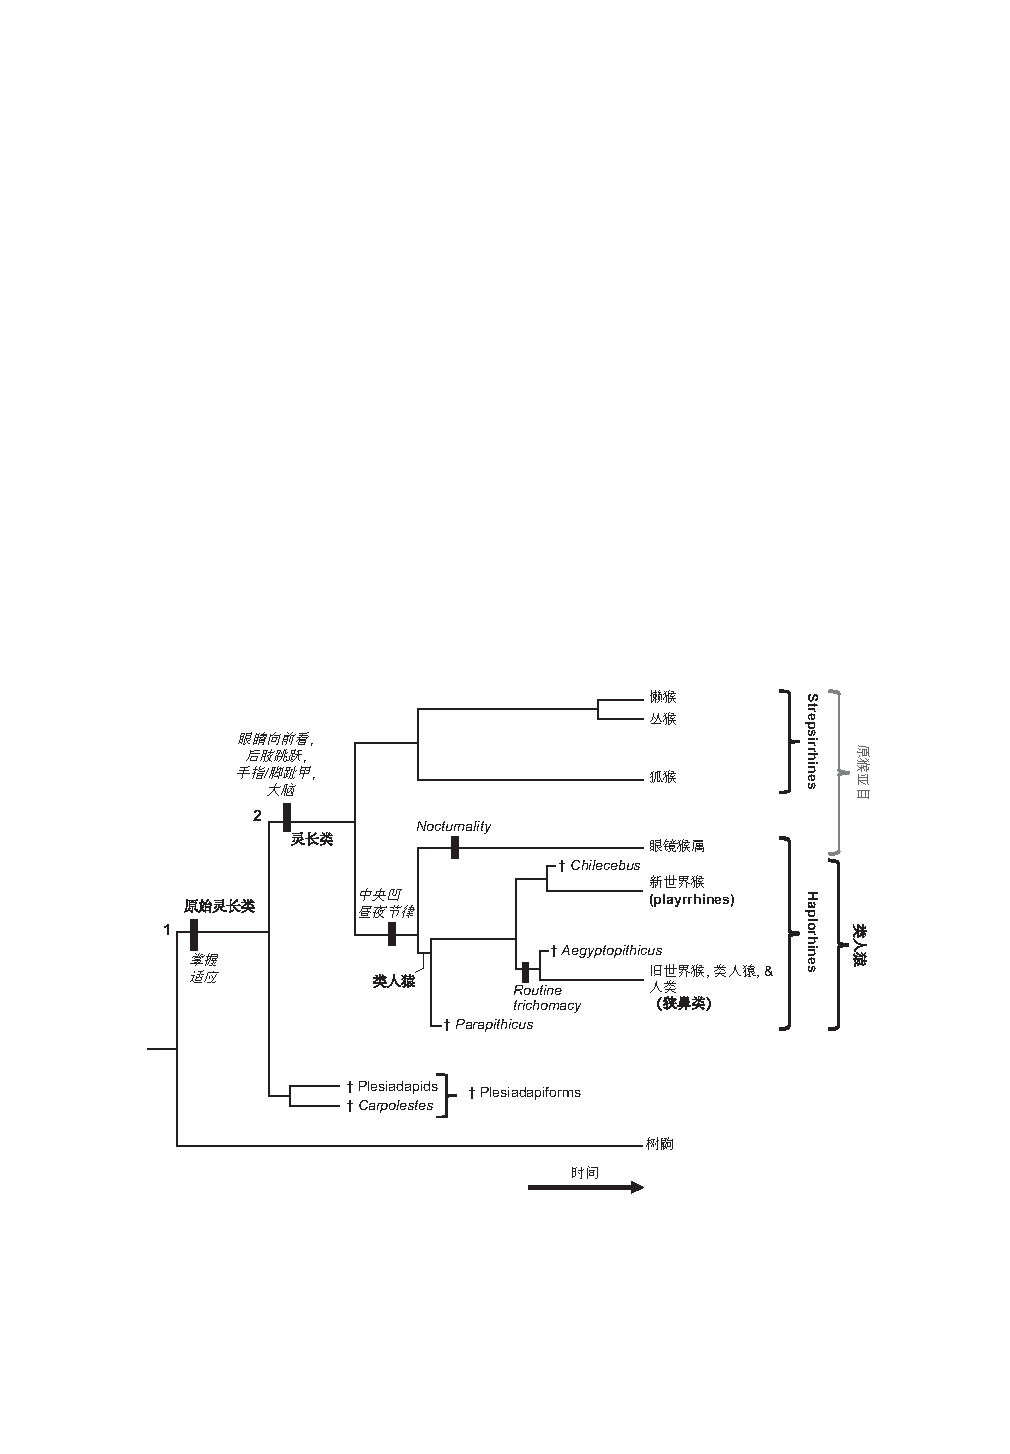
\includegraphics[width=0.8\linewidth]{chap2/2_5}
	\caption{所选现代灵长类动物和灭绝灵长类动物之间的进化关系。
		黑色条纹表示某些分支线路的创新,每个条纹旁标有斜体字注明创新特征。
		右侧方括号中的组,黑色表示自然群(类群),灰色表示其他(近源)群。
		†表示已灭绝的群体。
		1和2表示关于灵长类动物最近共同祖先的不同观点。\label{fig:fig_2_5}}
\end{figure}


\begin{figure}[!htb]
	\centering
	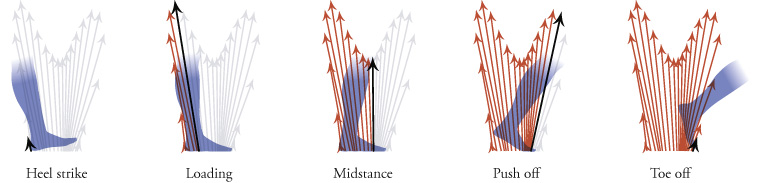
\includegraphics[width=0.8\linewidth]{chap2/2_6}
	\caption{选定的灵长类物种和树鼩之间的进化关系。
		缩写:IT,颞下皮层;PF,前额叶皮层;PM,前运动皮层;PP,后顶叶皮层;SMA,辅助运动区。
		每个末端圆圈的直径与包括颗粒前额叶皮层的皮层比例成比例,所选物种的百分比标在每个圆圈右侧。
		格式与图~\ref{fig:fig_2_5}~相同,只是时间尺度是线性的。\label{fig:fig_2_6}}
\end{figure}


通过比较一个代表性的猴形目灵长类动物(如猕猴)与一个代表性的原猴亚目动物(如灰背树鼩)的大脑,我们可以得出第二组结论。
图~\ref{fig:fig_2_5}~展示了这些灵长类动物的关系,以及随着某些谱系的出现而出现的特征,这些特征可以在黑色条形上方或下方找到。
图~\ref{fig:fig_2_6}~指出了早期灵长类和猴形目动物中进化出来的一些皮层区域。\par


1.原猴类动物缺乏类人灵长类动物中存在的几个区域的同源,包括中侧前额叶皮层(区域46),背内侧前额叶皮层(区域9)和腹侧前额叶皮层(区域12/47)。
我们认为后外侧皮层(区域9/46)和\textit{额极皮层}(区域10)也属于这一类别,尽管这些点的证据仍不够全面;\par


2.这些新区域是在原猴类和类人猿亚目分裂之后进化出来的,可能是在人猿类中进化出来的,后文我们会解释;\par


3.原猴类和类人猿共享 2 组区域。
第一组包括所有哺乳动物都有的无粒界前额叶皮层区域;
第二组则对应于早期灵长类动物进化出来的有粒界前额叶皮层区域,其中包括额叶视区和颅后无粒界额叶皮层(区域8)的其他部分,以及眶上的有粒界前额叶皮层部分。



\begin{table}[htbp]
	\centering
	\caption{在哺乳动物、原猴类和类人猿中具有同源 (+) 或可能具有同源 (?) 的皮层区域}
	\setlength{\tabcolsep}{8mm}	
	\renewcommand\arraystretch{1.5}	
	\begin{tabular}{lllll}
		\toprule
		区域 & 来源 & 哺乳动物 & 原猴类 & 类人猿 \\
		\midrule
		背内侧皮层 & a & & &+  \\
		中侧皮层 & a & & &+  \\
		腹侧皮层 & a & & &+  \\
		尾部主要运动皮层 & b,c & & &+  \\
		后外侧皮层 & a & &? &+  \\
		\textit{额极皮层}&  a & &? &+  \\
		尾侧前额叶皮层&  a & &+ &+  \\
		前额眼区& a,c & &+ &+  \\
		颗粒状\textit{眶额皮层}& a & &+ &+  \\
		前运动皮层& c & &+ &+   \\
		腹侧前运动皮层& c,d & &+ &+  \\
		背侧前运动皮层& c,d & &+ &+  \\
		辅助运动区& c,e & &+ &+  \\
		扣带回运动区& c,e & &+ &+   \\
		颞下皮层& f & &+ &+   \\
		后顶叶 & f,g & &+ &+  \\
		颞前皮层 &  b,c &+ &+ &+  \\
		前扣带回 &  h &+ &+ &+  \\
		下肢前额叶皮层 & h &+ &+ &+  \\
		前枕皮层 & h &+ &+ &+  \\
		无粒界颞叶前额叶皮层 & h &+ &+ &+  \\
		无粒界岛叶皮层 & h &+ &+ &+  \\
		周边海马皮层 & i &+ &+ &+  \\
		\bottomrule
		\label{tab:tab_2_2}
	\end{tabular}%
\end{table}%


表格~\ref{tab:tab_2_2}~总结了这些结论,并添加了一些前额叶皮层以外的区域,包括一些超出额叶的区域。
除了新的前额叶皮层外,灵长类动物还在后顶叶、前运动皮层和颞叶皮层进化了新的区域。
这些进化已经在其他地方进行了审查\cite{kaas2020evolution,preuss2007primate}。


一些较大的不确定性值得讨论。
对于11区,也就是眶额皮层最前端的部分,我们使用“可能”这个词。
Preuss\cite{preuss1991myelo}认为他们可以在灵长类动物中识别出11区的同源区,但置信度较其他区域低。
对于后外侧额叶皮层(9/46区)和极端额叶皮层(10区),也存在类似的问题。如果灵长类动物存在后外侧额叶皮层的同源区,那么将其包括在尾部额叶皮层中是有意义的,正如我们在第~\ref{chap:chap5}~章中所做的那样。
未来对多种灵长类物种的研究应该能够澄清这些问题。


这些证据表明,灵长类大脑皮层在进化过程中发展了新的区域。
声称其他哺乳动物(如老鼠)的额叶基本上是灵长类大脑皮层的缩小复制或融合,不仅与比较证据相矛盾,而且也缺乏可信性。
灵长类大脑皮层发展了十几个新的视觉区域以及许多新的后顶叶和前运动区域,这些有着令人印象深刻的证据支持。
缩小复制理论认为,在新皮层大区域中,仅额叶皮层未在灵长类进化过程中发展新的区域。
融合理论认为,老鼠的少数额叶皮层区域具有灵长类大脑皮层的所有特性和功能。我们可以否定这两种想法。


因此,我们得出结论:无论是在结构还是功能上,颗粒状前额叶皮层都是灵长类动物的一项创新。
这个想法得到了最近一项关于发育中人脑基因表达的分析的进一步支持。
在对灵长类和啮齿类特异基因的比较中,Zhang等人\cite{zhang2011accelerated}发现,在发育过程中,颗粒状前额叶皮层表达了198个人类或类人猿特异基因,作者认为这些新基因起源于灵长类动物,以调节大脑的生长。


这不仅是灵长类动物进化出新的前额叶区域,而是作为一系列灵长类创新的一部分发展而来,其中包括新的运动前区、后顶叶、颞叶区域,以及与它们相连的丘脑和纹状体的主要部分\cite{preuss2007evolutionary,preuss2007primate}。



\section{腹侧前运动皮层}

如果灵长类动物发展了一系列新的皮层区域,那么仅关注前额叶皮层就是一个错误。
后面我们会提出,他们的颗粒状前额叶皮层使早期灵长类动物采用了一种新的方式寻找食物并在特定的环境中进行选择。
但是,这种发展需要在全新的视角、新的移动方式、新的触角,以及新的摄食方式的背景下加以理解。
灵长类动物视觉和运动的进步非常明显,因此我们在下面的章节中只简要提及它们。
然而,灵长类动物触角和摄食的方式需要更多的解释。
因此,本节重点介绍了支持这种能力的一个关键区域:腹侧运动皮层。


Nudo\cite{nudo1988descending,nudo1990descending}发现,在他们研究的所有灵长类动物中(包括半猴亚目、新大陆猴和旧大陆猴),锥体束的投射都起源于 3 个皮层区域(表~\ref{tab:tab_2_1})。
他们研究的灵长类动物包括灰鼠狐、慢浆猴、松鼠猴、普通狨、绿猴和猕猴。
在每种灵长类动物中,Nudo和Masterton都能够识别一个锥体束细胞群,其起源对应于腹侧运动皮层。


他们在检查了一定数量的哺乳动物物种之后,未能在任何15种非灵长类哺乳动物中找到同源区域。
这项比较研究表明,腹侧运动皮层及其皮层脊髓投射在早期灵长类中进化。


猕猴的腹侧运动皮层含有约5\%的皮层脊髓神经元\cite{dum2004motor},并且它们的脊髓终止的分布与大多数其他运动区域不同。
腹侧运动皮层的脊髓投射主要终止于颈椎脊髓的上部(头端),这些运动神经元控制颈部和肩部肌肉以及呼吸。
大多数其他运动区域投射到脊髓的几乎所有水平,并控制整个身体。
腹侧运动皮层还投射到面神经核,这是一个位于脑干的运动核,特别是控制下半脸、嘴唇和下颌肌肉的部分\cite{morecraft2001cortical}。


根据不同前运动区的连接,已经确认了腹侧运动皮层在阔鼻灵、平鼻灵和窄鼻灵灵长类动物中的存在\cite{kaas2004evolution}。
灰毛猴、卷尾猴(Cebus)\cite{dum2004motor}、夜猴(Aotus)\cite{preuss1996movement,gharbawie2010thalamocortical}、松鼠猴(Saimiri)\cite{cowey1968varying}、普通狨猴(Callithrix)\cite{burish2008microstimulation}和猕猴\cite{lu1994interconnections}都有连接原发性运动皮层以及后部顶叶皮层的腹侧运动皮层。
与皮层脊髓束的连接一样,这些皮层间连接表明腹侧运动皮层在早期灵长类动物中进化而来。


这个创新的重要性在于它与早期灵长类动物适应的生态位有关。
早期的灵长类动物沿着小树枝移动,一只手用于抓住树枝,另一只手用于取食。
在后代灵长类动物中,比如猕猴,腹侧前运动皮层继续在抓取和握持中发挥作用。
例如,这个区域的失活会影响动物根据所看到的物体大小校准其抓握大小的能力\cite{fogassi2001cortical}。


\subsection{小结}

腹侧前运动皮层在早期灵长类动物中进化形成,伴随着颗粒前额叶皮层、颞叶和顶枕叶的新部分的出现。
根据它与脊髓的连接,腹侧前运动皮层似乎在控制口部、头部和伸手运动方面发挥作用,而不是后肢的运动。我们把这种专门化看作是一种线索,表明这些新区域的进化与前肢为基础的觅食有关。
虽然它们没有直接投射到脊髓,但其他的前运动皮层区域也具有前肢的专门表征,而非后肢。
这些区域包括前背外侧皮层和背侧前运动皮层的前部。
在接下来的章节中,我们将重建早期灵长类动物的生态位,并解释它们如何通过视觉、运动和伸手的进步来适应它。



\section{早期灵长类动物}

化石证据表明,灵长类动物的进化包括可对立的拇指或大趾,用于抓握的手和脚,这些手和脚上的大多数指头有指甲而非爪子,以及前向定向的眼睛\cite{fleagle2013primate,rose2006beginning}。
由于我们的前向定向眼睛,研究灵长类动物大脑的大部分文献都集中在视觉系统的适应性上,包括上优结节,外侧膝状核和几个新的视觉皮层区域。
所有这些适应性已经被详细讨论过\cite{barton2004binocularity,kaas2020evolution,preuss2007evolutionary}。
然而,这些特征本身对于我们了解颗粒前额叶皮层提供的优势并没有太多作用。
为了理解颗粒前额叶皮层对早期灵长类动物产生的影响,我们需要了解它们如何谋生。


我们提出早期灵长类动物及其近亲发展出了一种新的觅食方式,涉及前额叶皮层。
这种新的觅食方式包括一系列的适应性,用于寻找、选择、移动、伸手取食和摄食早期灵长类动物在被子植物细小枝条上发现的食物。
事实上,灵长类动物与被子植物之间的密切关系导致一些专家认为,灵长类动物进化是为了利用被子植物的适应性辐射。


在细小的树枝上觅食涉及身体和大脑的许多特化,我们认为这些生态因素解释了新的颗粒状前额叶皮层区域及其功能的出现。
我们并不否认社交群体的性质对灵长类动物大脑的演化有影响\cite{dunbar2009social},但早期灵长类动物可能在分散的社交系统中相对独居\cite{mueller2000origin}。


早期灵长类动物的觅食方式可以从 Bloch\cite{bloch2002grasping}对生活在约5500万年前的食果猴化石的研究中推断出一些想法。
图~\ref{fig:fig_2_5}~显示了这些动物与现代灵长类动物之间的关系,表2.1列出了一些关键术语。
早期灵长类进化的两种观点已经形成。
一种认为以“1”标记的物种的后代是灵长类;
另一种将灵长类(常称为现代形态的真灵长类或灵长类)视为标有“2”的谱系的后代。
我们不需要在这些观点之间进行选择。只要知道食果猴是早期灵长类动物的近亲就足够了,即便它不是早期灵长类动物本身。


Bloch和Boyer得出结论,食果猴具有许多促进肢体抓握的特征,但缺少一些现代灵长类的特征。
特别是,食果猴缺乏更朝前的眼睛和明显的跳跃能力。像灵长类的近亲树鼩(Tupaia)一样,食果猴的眼睛朝向侧面。
如前所述,化石和现代灵长类的眼睛都朝向前方。
Bloch和Boyer还得出结论,食果猴的后腿和骨盆不能支持有效的跳跃。
基于此,他们得出结论,一种专门的抓握能力在现代灵长类中表现为面向前方的眼睛和跳跃能力的进化。
Bloch和Boyer还得出结论,食果猴的抓握专门化使它们能够利用细枝巢位。


细小枝条生态位包括了生长在被子植物树木边缘的资源。
最细、最小、最远端的枝条上有大量含有营养的花朵,其中包含有营养的花蜜。
果实、坚果和种子提供了大量的营养价值,它们就生长在花朵所在的细小枝条上。
细小的枝条也有许多最鲜嫩的叶子,与老叶相比,动物可以更有效地消化这些叶子。
灵长类动物更喜欢嫩叶,因为这些叶子相比成熟的叶子蛋白质比例更高,纤维素比例更少。


Cartmill\cite{cartmill1974rethinking}和Martin(1990)也得出结论,早期灵长类动物适应了细小树枝的生态位,但与Bloch和Boyer的研究不同的是,他们强调适应视觉导向运动的适应性(Martin 1990)或视觉介导的对昆虫捕食的适应性\cite{cartmill2017arboreal,bloch2002grasping},而不是对果实、花朵和花蜜的利用\cite{sussman1991primate,bloch2002grasping}。
在这种观点中,抓握专业化、前向眼睛和后肢支配的跳跃结合成为在昏暗的树枝上觅食的适应性,早期灵长类动物通过跳跃和抓握在这些树枝上移动。


正如 Jenkins\cite{jenkins1974tree}指出的那样,许多哺乳动物物种利用细小树枝这个生态位,松鼠在其中占据显著位置。
因此,如果早期灵长类和它们的祖先在被子植物树的细小树枝上争夺资源,它们则需要一些优势。
Jenkins 提出这种优势涉及在细小树枝上生活,而不是偶尔进入该生态位。


生活在细小树枝上存在许多挑战。无论早期灵长类动物主要寻找什么食物——昆虫、嫩叶、水果、花蜜、种子、坚果或花朵——它们都必须在细小树枝间移动、有效地选择食物并在不摔落的情况下食用。


在接下来的部分中,我们将回顾灵长类为了能够利用细小树枝栖息地而发展出的视觉和运动专业化。
在本节末尾,我们提出,它们新的颗粒状前额叶皮层区帮助早期灵长类发现和选择细小树枝栖息地中的高价值食物。
为了理解这个建议,我们需要欣赏导致新的观看、移动、伸手和进食方式的整套适应性。
灵长类常被称为“视觉动物”。
我们没有使用这个模糊的短语,但那些使用它的人无疑不是指其他动物不能看见。
相反,他们打算强调视觉在灵长类行为中的主导地位。
即使在没有显然原因的情况下,视觉在灵长类中占主导地位。
在觅食中,视觉占主导地位(本章),在寻找和关注食物时,视觉占主导地位(第~\ref{chap:chap5}~章),在学习选择食物方面,视觉占主导地位(第~\ref{chap:chap4}~章)。
只有理解对细小树枝栖息地的整个适应性集合,才能完全理解颗粒状前额叶皮层带来的优势。



\subsection{灵长类动物的视觉方式}

比较神经科学家们强调了灵长类动物视觉方面的进步,这是有充分理由的。
然而,要理解它们对于新皮层前区的起源的贡献,我们需要认识到早期灵长类动物的视觉与许多现代灵长类动物(包括人类)的视觉有何不同。


我们对视觉的直觉来自于我们的经验,这主要由明亮环境中的视网膜中央凹视力组成。
因此,很自然地认为早期灵长类的视力依赖于聚焦、高分辨率、明亮光线下、凹视力依赖的彩色视力。
但是早期灵长类的视觉没有这些特性。
早期灵长类缺乏视网膜中央凹,而是在夜间、昏暗的光线下觅食。
因为它们缺乏视网膜中央凹,所以前向的眼睛和大的双眼视野的发展与人类和其他现代灵长类所具有的凹视力无关。
相反,早期灵长类的前向眼睛必须进化为在昏暗光线下的视觉,既没有凹视力介导的高分辨率,也没有人类(和其他旧大陆灵长类)具有的那种彩色视力。


更朝前的眼睛产生的大视场可以为立体视觉和深度感知产生更大的视场。
Barton\cite{barton1998visual}表明,现代灵长类的大脑大小和视觉皮层大小与前置眼方向的程度相关,他将这些特征归因于双眼视觉,特别是增加的立体视场的重要性。
在细小的分支环境中跳跃和伸手够食物时,立体视觉显然非常重要\cite{cartmill1974rethinking}(CMartin 1990)。


但是双眼视觉不仅具有立体视觉的优势。它可以通过两只眼睛输入神经元的叠加促进在昏暗光线条件下的敏感性\cite{crescitelli1977topography,allman1999evolving},并且它允许至少一只眼睛绕过复杂树枝环境中遇到的障碍物,看到远距离物体(Changizi 2009)。
面向前方的眼睛还提供了更广阔的视野和深度感知,可以在空间下方和前方的头部进行重要的伸手和操纵物体\cite{barton2004binocularity}。
正如Barton所指出的那样,具有侧向眼睛的动物存在问题。
眼眶颅骨限制了它们对临近物体的凝视能力,尤其是那些位于头部下方的区域,这些区域通常是需要精细操纵的位置。
早期灵长类动物的面向前方的眼睛可能有助于克服这个问题。


因此,早期灵长类动物前向眼睛可能在多种方面帮助它们识别和获取食物,包括在昏暗光线下增强感受力,更好地观察障碍物周围的视野,提高头部以下区域的视觉能力以及改善深度感知。



\subsection{灵长类动物的运动方式}

灵长类动物的行动方式与其他哺乳动物也有所不同,这也反映了它们生活在细枝细节的环境中。
为了应对在纷繁的细枝上移动和觅食时所遇到的困难,需要进行多项适应。


生活在和在细小树枝之间导致了步态的变化。为了在细小树枝环境中进行树栖运动和觅食,灵长类动物使用了与其他哺乳动物不同的肌肉收缩模式\cite{larson1998unique}。
关键差异包括后肢和前肢的推力较小以及前肢的硬度较小\cite{schmitt2010primate}。
灵长类动物使用的低力量限制了它们在树枝上移动时产生的摆动,否则可能会吸引捕食者。


早期的灵长类动物与非灵长类动物相比,使用了不同的肌肉协调模式来适应在细小分支环境中的树栖运动和觅食。
尤其是,灵长类动物的运动主要由后肢驱动,这种后肢为主导的运动方式为前肢腾出了更多的功能,如稳定、转向、抓握和操纵等。
这种运动方式也使得手到口的进食成为可能,一只手提供稳定,另一只手伸向食物并将其送入口中。
这种新的觅食方式涉及到早期灵长类动物出现的新的前运动皮层和新的前额叶颗粒皮层。
首先,我们会讨论腹侧前运动皮层。



\subsection{灵长类动物的接触和进食方式}

为了理解腹侧运动层的重要性以及早期灵长类动物为何需要新的功能区域,我们需要认识到在细小枝条环境中进食并不轻松。
在野外进食时,采食者和食物都可以保持静止。
在细小枝条环境中进食则面临更为严峻的挑战。
早期灵长类动物必须掌握在脆弱平台上的身体稳定性,同时伸展身体去获取相对于身体运动的食物。
即使在它们抓住了想要吃的食物后,这些动物在保持在薄薄的、柔软的树枝上的平衡的同时将食物送入嘴里仍面临着严重的问题。


腹侧前运动皮层及其对脑干和脊髓的投射可能有助于解决树栖生活中的这些问题。
Nudo\cite{nudo1990descending}寻找该区域的皮层脊髓投射和各种运动行为(包括手部灵巧和手眼协调等方面)之间的相关性。
他们发现这些因素之间几乎没有相关性。
相反,他们发现腹侧前运动的相对大小与树栖生活显着相关。
这种相关性并没有告诉我们腹侧前运动皮层如何对这种生活做出贡献,但似乎有助于手到口的伸展和进食。


正如我们之前提到的,来自腹侧前运动皮层和脑干的皮层脊髓束和脑干投射结束于控制头部、肩膀、下颚和唇部肌肉的运动神经元上,而不是控制躯干和后肢肌肉的运动池上。
这些特征表明,腹侧前运动皮层在灵长类动物的前肢、头部和口腔运动中扮演更重要的角色,而不是后肢主导的运动。
前肢、头部和口腔运动组合在手到口的进食中。将手移向口腔进行进食需要手、头部和口腔的协调定向,而腹侧运动皮层可以提供这种控制\cite{preuss1993role}。


电刺激皮层的证据也表明,腹侧前运动皮层在手到口的喂食中起着重要作用。在猕猴中,Graziano等人\cite{graziano2002cortical}对腹侧前运动皮层进行了几秒钟的电刺激。
这种刺激引起了手的握合,同时手移向嘴巴。
它还引起了嘴巴的张开和头部的运动,使其转向手的位置,因为手靠近嘴巴。
因此,皮层刺激人为地引发了喂食行为。
在其他灵长类动物的后部顶叶皮层和前运动区也可以引发类似的效果\cite{stepniewska2009organization,gharbawie2010thalamocortical}。


在解决在不稳定、摆动的支撑物上将食物送入口中的问题的同时,伸手到细小分支领域获取食物还需要保持姿势的稳定。
MacNeilage等人\cite{macneilage1987primate}指出,现代原猴亚目使用单手狩猎昆虫的捕食技巧,其中一只手用于保持姿势支撑,而另一只手则伸向食物并将其送到嘴里。


为了完成这项壮举的一种运动控制策略是:无论树枝如何摇晃,保持肩膀在一个固定的位置。
腹侧前运动皮层对控制肩胛骨肌肉的投射可能会弥补由基底不稳定性引起的意外身体运动。


另一种策略涉及不断计算手的当前位置与食物之间的差异。
通过这种方式,即使身体摇晃且食物因风或动物对树枝的影响而移动,当手运动接近食物时,运动指令也会自动调整。
Wise\cite{wise2007evolution}总结了这些结论的证据。


综合神经生理学和心理物理学证据表明,灵长类动物已经进化出了独特的伸手方式。Shadmehr\cite{shadmehr2004computational}在一本书中论述了这个结论,但我们在这里介绍他们的一些关键发现:\par

1.灵长类动物的伸手能力发生在视觉参考系中(见图~\ref{fig:fig_5_3})。
有些细胞在视网膜坐标系中编码目标的位置,而其他细胞则以相同的坐标系编码手的位置。
乍一看,运动控制系统只需要手和目标之间的空间关系。
仅凭这些信息,就可以确定关节角度变化和力的大小,将手伸向目标。换句话说,伸手似乎只需要身体中心坐标系,也称为以自我为中心或本体参考系(第~\ref{chap:chap3}~章)。
灵长类大脑不需要将伸手运动编码成视网膜参考系,但证据表明它确实这样做。
例如,腹侧前运动皮层的细胞活动更好地反映外在视网膜坐标系中的运动轨迹,而不是内在的运动坐标系;\par


2.灵长类动物在计算伸手的目标点和当前手的位置时使用视网膜坐标系,这使得他们每次眼睛移动时都需要重新计算运动计划。
没有显而易见的原因需要这样重新计算。
当眼睛改变其方向,但伸手目标和手仍然保持不变时,运动指令不需要改变。
然而,灵长类动物的大脑每次眼睛移动并且在眼睛移动之前都要重新计算目标位置、手的位置和运动计划;\par


3.实验表明,人类大脑以视觉参考系计算伸手触及目标,即使是声音目标也是如此。
如果目标位于人的外围视野中,人们会略微超过目标。
对于视觉目标,这是有道理的,因为外围视觉有一些固有的不准确性。
然而,对于声音目标,这种不准确性也会出现在伸手触及时,尽管没有必要考虑到视网膜的属性;\par


4.先天失明的人进行视觉引导的运动时,比视力正常的人更能直接、准确地完成,这种现象是因为视力正常的人会受到微小的视觉扭曲的影响。


这些发现表明,视觉在灵长类伸手取物的过程中占主导地位。
在早期灵长类动物中,它们新进化出的前运动皮层和后顶叶区域以视网膜参考系执行了伸手取物的计算,这些区域的同源物在其后代中也是如此。
随后我们会认为,视觉也主导了寻找和选择食物的过程,并且新进化出的\textit{腹侧前额叶皮层}支持这些功能。


由于腹侧前运动皮层会产生达到目标的伸手命令,因此并不奇怪它有一些称为镜像神经元的细胞,这些细胞编码目标实现的方式,无论谁或什么实现该目标 \cite{umilta2001know}。
腹侧前运动皮层还在协调头部和手部运动方面发挥作用。
通过执行这些功能,腹侧前运动皮层有助于解决早期灵长类动物在精细树枝巢穴觅食时遇到的两个问题:到达食物并将其带到口中。



\subsection{灵长类动物的寻找和选择方式}

适应于细小树枝环境的成功不仅需要改进视觉引导的跳跃、伸手和抓握能力。我们认为,视觉在早期灵长类动物中占据着主导地位,这促进了它们改进搜索食物和评估在复杂树枝环境中发现的食物价值的方式。
早期我们提到过灰质前额叶皮层的某些部分在早期灵长类动物中进化。
在这里,我们提出这些新的灰质前额叶皮层区域在早期灵长类动物中介导了搜索和估值功能,并在现代灵长类动物中继续执行这些功能。


根据本章第一部分总结的灵长类动物的研究证据,我们接受了Preuss的结论,即早期灵长类动物拥有两个颗粒状前额叶皮层的同源物:尾侧前额叶皮层(区域8),其中包括额叶视区,以及颗粒状眶额皮层,包括区域11和13、14的颅部部分。


这两个区域都接收到强烈的视觉输入。
额叶视区与早期(低阶)视觉区域(如V2和V3)有广泛的联系\cite{stanton1995topography},而颗粒状眶额皮层与颞下皮层和带状回皮层有相当大的联系\cite{saleem2008complementary}。


第~\ref{chap:chap5}~章提出,\textit{尾侧前额叶皮层}提供了一种搜索食物和食物的视觉信号的机制。
它还在注意到这些物品方面发挥作用,包括潜在的注意力和显性的注意力(眼动)。
第~\ref{chap:chap4}~章提出,颗粒状的\textit{眶额皮层}编码食物的当前价值,并将以前的觅食选择与随之而来的结果(包括特定食物和液体的视觉特征)联系起来。
高价值的物品因此成为达到、抓取、操作和进食动作的目标。



\subsection{小结}

早期灵长类动物进化出适应在被子植物树上进行细枝夜间觅食的生态位。
它们具有前向的眼睛,但没有中央凹或全色(三色视觉),但具有大的双眼视野,使它们能够在昏暗、杂乱的环境中良好地运作,通过深度感知计算距离,并将两只眼睛对准头部下方的区域来操作物体。
随着前肢被新的灵长类动物的行动方式所解放,早期灵长类动物能够在视觉参考系中伸手取食物,并将其送到口中而不摔倒。
为了利用视觉的进步,新的后枕叶和前运动区域进化出来以控制灵长类动物的取食方式。


除了上面提到的进步之外,早期灵长类动物还需要在细小枝叶的生态位中搜索可取的食物,并评估其当前的生物学价值。
他们新进化出的颗粒质前额叶皮层为执行这些功能提供了优势,就像它们的后代动物的同源物一样。



\section{类人猿前额叶皮层}

到目前为止,我们已经关注了早期灵长类动物的进化,它们发展出了第一批颗粒状前额叶皮层区域。
后来灵长类动物的进化产生了类人猿,其中一些灵长类动物进化出了额外的颗粒状前额叶皮层。


如前所述,Preuss\cite{preuss1991myelo}对比了一个典型的原猴类(灵长目的一种,小灵猫)和一个典型的类人猿(猴属的一种,短尾猴)的前额叶皮层,发现类人猿进化出了几个新的前额叶皮层。
在我们的术语中(参见图~\ref{fig:1_4}),这些新区域包括中侧前额叶皮层(区域46)、背内侧前额叶皮层(区域9)、腹侧前额叶皮层(区域12/47)和可能的额极皮层(区域10)。
本章的下一部分探讨这些新区域何时出现以及可能导致它们发展的选择性压力。


图~\ref{fig:fig_2_5}~说明了许多现生灵长类动物之间的关系,还包括一些只在化石中发现的已灭绝灵长类动物。
表\ref{tab:tab_2_1}列出了一些关键术语。
Kay等人将类人猿亚目和半猿亚目的分化时间定为不少于5500万年前\cite{kay2004anthropoid}。
他们估计,类人猿和狐猴目的分化时间约为4500万年前,旧大陆猴和新大陆猴的分化时间约为3400万年前。
为了将这些值放在适当的背景下,灵长类动物首次出现约为6500万年前,类人猿和其他旧大陆灵长类动物的分道扬镳发生在约2300万年前,人类和黑猩猩的分化线路发生在约700万年前。


下一节中所解释的比较证据表明,早期的半猴类从它们的直系祖先所采用的夜间觅食习惯转变为了昼行性生活。
它们还发展出了更前方的眼睛定位和真正的视网膜凹,这导致了视力的提高。
在分化成新大陆和旧大陆人猿之后,旧大陆人猿进化出了人类所具有的三色(三色)视觉\cite{williams2010new}(deValois\&Jacobs 1998)。
这种常规的三色视觉与新大陆猴类中发生的多态性三色视觉不同,这是我们稍后将讨论的主题。


许多关于人猿类皮层进化的研究都着重于视觉区域的增多\cite{kaas2020evolution},而前额叶皮层则受到较少的关注。
然而,像大视皮层、前置眼、和凹点一样,大额叶是现代人猿类的显著特征。
正如我们稍后所述,他们的大额叶主要反映了大的颗粒前额叶皮层。



\subsection{生态因素}

前额叶皮层的变化是因为从夜间活动转变为白天活动对人猿类的影响深远,不仅仅是视觉方面。
这种变化影响了类人猿的大小、移动方式、饮食和生态位。
随着时间的推移,类人猿变得更大,适应了原始灵长类动物的运动方式,成为树栖四足动物,并且开始依赖除了细枝生境以外的被子植物树的产品。
早期类人猿及其后代面临了新的竞争对手和更高的捕食风险,这是白天生活带来的,也面临来自彼此之间的竞争。


或许对于颗粒状前额叶皮层来说最重要的是,随着类人猿的进化,它们也不得不应对食物需求的明显波动,即使是在类人猿进化和现今生活的繁茂热带环境中,也会有食物短缺的间歇性时期\cite{jf1987food}。



\subsection{社会因素}

转为日间觅食增加了捕食的风险,人猿可能通过成群生活来适应捕食。
除了其他的优势外,有很多眼睛可以观察捕食者。
由于这些新的社会结构,人猿不仅需要关注觅食,还需要考虑与其他群体成员的互动。
这些因素也会对大脑的进化产生影响,尤其是对前额叶皮层的影响。


一些最近的证据指出,新进化的颗粒状前额叶皮层域的某些部分,以及前额叶皮层的其他部分,在社交选择中起到了作用。
最近的研究结果表明,随着猕猴在越来越大的社交团体中互动,中侧前额叶皮层的大小也会增加\cite{sallet2011social}。


颞上沟内的一个区域随着社会群体的扩大而增大。该区域的细胞对灵长类的凝视角度和面部方向做出响应\cite{perrett1985visual},以及对其观察到的动作做出响应\cite{jellema2003cells}。
这一发现与前额叶皮层有关,因为这个颞上区域投射到前扣带回皮层,这是前额叶皮层的一部分(第\ref{chap:chap3}章)。
并且,与这个投射相一致,社会群体越大,颞上区域的激活与前扣带回皮层的激活之间的协方差越大\cite{sallet2011social}。
这一发现有两个有趣的原因。
首先,Yoshida等人\cite{yoshida2011representation}报告了在中央前额叶皮层中区分自我和他人的细胞;这些细胞在社会环境中编码另一个代理的动作。
其次,Rudebeck等人\cite{rudebeck2006role}发现,前扣带回回旋部有损伤的猕猴对其他猕猴的图片不再感兴趣,即使这些图片描绘了一个对着它们以威胁的方式盯着它们的猕猴。
第\ref{chap:chap9}章将继续讨论与人脑相关的这一问题。



\subsection{小结}

类人猿从其半猴亚目的祖先那里继承了白天觅食的习性,并随着时间的推移变得更大。
比较证据表明,随着它们的体型增大,它们进化出了新的前额叶皮层。
在下一节中,我们将回顾证据,说明在类人猿进化过程中,它们开始依赖不稳定的资源。
它们成为了体型较大的动物,没有储存食物的能力,并在更大的社会群体中觅食。
因此,不良的觅食选择会浪费它们的时间和精力,尤其是在食物短缺的时期。
考虑到捕食的风险和有限食物的竞争,类人猿进化出了比它们的祖先更有效地觅食的能力。
我们后来会提出,它们新的颗粒状前额叶皮层有助于减少冒险或无效的觅食选择。



\section{祖先类人猿和高级类人猿}

根据内骨模印象显示的大脑结构,我们可以得知早期类人猿的大脑额叶相对较小\cite{radinsky1979fossil}。
通过研究灭绝灵长类物种的内骨模印象,Radinsky发现在类人猿演化的很长一段时间内,这些动物的额叶都很小。
图\ref{fig:fig_2_7}A显示了一种已灭绝的类人猿物种埃及古猿的化石内骨模印象,它是一种早期的猫猴类灵长目,生活在约3300万年前\cite{kay2004anthropoid}。
埃及古猿有一个显眼的中央沟,但它的前额叶皮层却很少,这与现代人猿的情况不同。
基于这些证据,Radinsky得出结论,额叶的扩张发生在人猿的视觉区域扩张之后。
根据他的分析,视觉皮层的扩张始于大约5500万年前的早期灵长类演化阶段。
到了埃及古猿时期,视觉皮层的扩张已经达到了现代人猿的范围,但额叶仍然相对较小。


\begin{figure}[!htb]
	\centering
	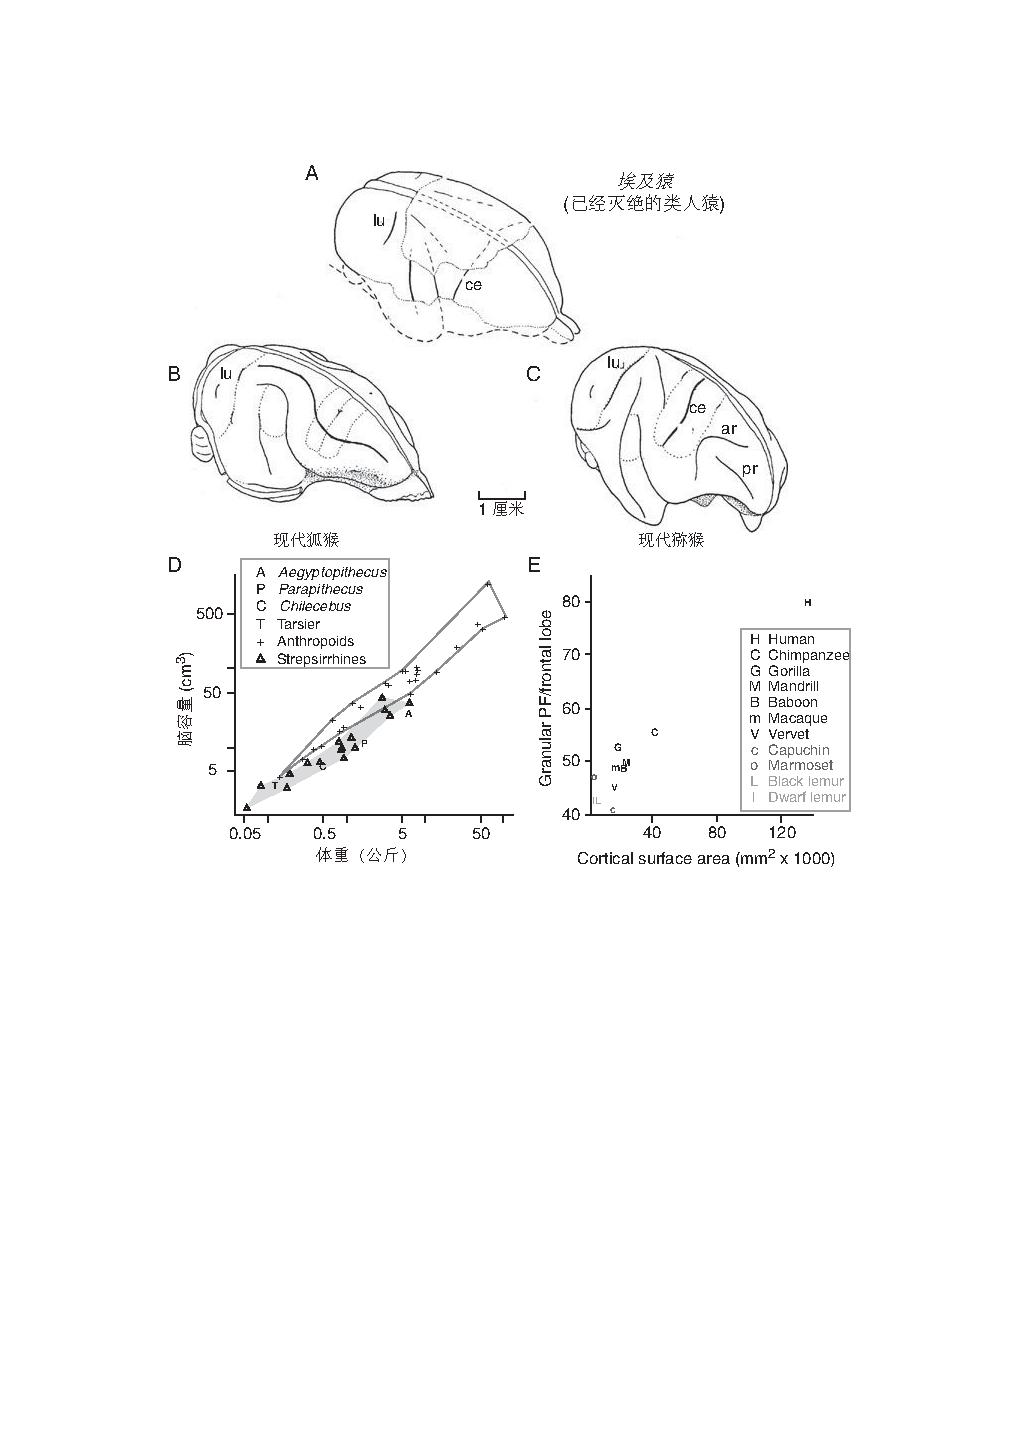
\includegraphics[width=0.8\linewidth]{chap2/2_7}
	\caption{(A-C)是已灭绝的类人猿动物埃及长颈猿的化石内脑凸与现代的原猴(B)和恒河猴(C)进行比较。
		正前方朝右,背部向上。
		缩写:ar,弓形沟; ce,中央沟; lu,月状沟; pr,主沟。
		图(B)和(C)中的虚线指示自尾到头的大致位置:主要视觉、主要听觉、主要体感和主要运动区域。
		(D)所选已灭绝和现代灵长类动物的脑大小与体大小之比。
		缩写:A,埃及长颈猿; C,智利狨; P,帕拉猴; T,狐猴。 
		(E)额叶小叶颗粒前额叶皮层占前额叶皮层(表面积)比例随皮层大小变化的百分比。
		(A-C)转载自Radinsky L. 1975. Primate brain evolution. American Scientist 63:656–63。 
		(D)修改自Bush EC、Simons EL、Allman JM.高分辨率计算机断层扫描研究化石人猿帕拉猴头骨:对灵长类动物感觉系统演化历史的新见解。
		解剖学记录:综合解剖学和进化生物学的进展281a: 1083-7,2004,John Wiley and Sons,获得许可。 
		(E)修改自Elston GN、Benavides-Piccione R、Elston A、Zietsch B、Defelipe J、Manger P、Casagrande V、Kaas JH。灵长类动物颗粒前额叶皮层的特化:对认知加工的影响。
		解剖学记录:综合解剖学和进化生物学的进展288a:26-35,2006,John Wiley and Sons,获得许可。\label{fig:fig_2_7}}
\end{figure}


化石还表明埃及古猿的整个大脑大小。
现代类人猿的大脑大小超过了其体型大小预期的狐猴类靈長目动物。 Allman\cite{allman1999evolving}和 Streidter\cite{striedter2005principles}等人强调了这种类人猿特征,通常称为大脑大小的“向上分级转移”。
图~\ref{fig:fig_2_7}~说明了现代灵长类动物的这种向上转移。
它还显示了埃及古猿的大脑与体重的关系(图~\ref{fig:fig_2_7}~D中的点A)。
相对较早的狒狒亚科类人猿的大脑相对于其体型较小,在现代狐猴类靈長目动物的范围内。


图~\ref{fig:fig_2_7}D~还绘制了另一种灭绝的类人猿副猿\cite{bush2004high},这种类人猿接近最早的类人猿\cite{simons2004cranium}。
与埃及古猿一样,副猿(图~\ref{fig:fig_2_7}D~中的点P)的大脑处于灵长类身体大小的范围内,早期新大陆猴智利猴(图~\ref{fig:fig_2_7}D~中的点C)\cite{sears2008estimating}和Homunculus\cite{kay2006brain}也是如此。


根据图~\ref{fig:fig_2_7}D~中的点T,著名的灵长目动物夜猴的大脑也属于半猴类的范畴,这进一步证明了较小的“原猴”级别和较大的“类人猿”级别之间的区别。
早期旧大陆猴和新大陆猴的大脑大小在化石证据中显示出独立演化的趋势,考虑到它们相对较小的大脑,早期猫猴和早期扁鼻猴表明大脑的扩展独立进行。
因此,类人猿的大脑可能一直保持在半猴类的水平,直到大约在3400万年前扁鼻猴和猫猴分裂之后。


在本书的其余部分,我们将仅仅为了区分较大的后代物种与早期的、大脑较小的类人猿,将已经达到这种大脑上升档次的物种称为先进类人猿。
需要注意的是,在生物学中,先进一词仅仅意味着相对于祖先状态的某些分化,而原始一词仅仅意味着与祖先状态的密切相似。这些术语并不涉及相对能力或复杂性。
此外,由于我们对类人猿前额叶皮层的大部分了解来自于猕猴和人类这些猴类动物的研究,因此我们归因于先进类人猿的某些特征可能代表猕猴的专门化。


根据Radinsky的研究\cite{preuss2007primate},视觉皮层的扩展已经达到了现代类人猿的范围,而埃及古猿的大脑处于鼻猴大小范围内。
因此,相对较近的额叶扩张似乎是现代类人猿大脑增长的最大因素。
而且,像大脑总体扩张一样,这种额叶扩张似乎在旧大陆和新大陆猴类中独立发生\cite{williams2010new}。
因此,比例过大的额叶扩张可能产生了类人猿灵长类动物特征的大脑。


化石内窥镜无法区分颗粒和无颗粒前额叶皮层,但现代灵长类动物的细胞构造分析可以。
Brodmann\cite{brodmann1912neue}测量了现代灵长类动物颗粒前额叶皮层的大小,表明灵长类动物的大脑越大,新皮层中颗粒前额叶皮层所占的比例越大。
图~\ref{fig:fig_2_7}E显示了几种现存灵长类动物额叶皮层相对于新皮层的大小比例。
在代表性的类人猿中,颗粒前额叶皮层占新皮层的9-11\%,占额叶皮层的43-50\%(Elston等人,2006)。
代表性的原猴则对应的数值为7-8\%和41-43\%。
与颗粒前额叶皮层不同,颞皮层在大脑变大时并没有成比例地变大\cite{rilling2002quantitative}。
因此,在灵长类动物演化中,颗粒前额叶皮层似乎比其他大脑皮层部分成比例地扩展。
正如前面所解释的,比较解剖学的证据表明这种增加涉及前额叶皮层内新区域的发展。
当然,我们也不能排除类人猿额叶皮层其他部分的扩张。


这个结论表明,前期的类人猿甚至最早的猴形类动物的大脑皮层额叶皮层前区还没有发生扩张。
这一结论有一个重要的含义,即导致人猿类起源的选择性压力可能与导致后来类人猿产生新的颗粒状前额叶皮层区域的压力不同。
为了理解这些后来的选择性因素,我们需要更详细地考虑关键的人猿类创新。



\subsection{白天的生活和中央凹}

早期的半猴类动物转向了白天活动并进化出灵长类的中央凹,早期的类人猿遗传了这两个特征。
眼睛在早期类人猿中也采用了更前面的定位,并且在眼睛后方发展出一个眶骨作为下颌肌肉和眼睛之间的隔墙。


早期人猿类动物向日行性生活的转变以及灵长目中的“中央凹”的进化,为人猿类动物的日间行为提供了支持。
相对于大眼睛而言,小眼睛需要的光线更少,而所有早期类人猿动物的头骨都有相对较小的眶窝,这是白天生活的一个强烈指示\cite{fleagle2024primate}。
比较证据表明,几乎所有现代人猿类动物都有白天活动的模式,但很少有其他灵长类动物有这种模式\cite{heesy2004mosaic}。
早期人猿类动物继承了日行性生活,并且大多数仍然保留了这一特征。


凸眼动物视网膜窝的起源证据完全依赖于比较证据。
夜眼猴和类人猿的视网膜窝都具有许多共同特征。视网膜窝直径约为0.7毫米,每平方毫米约有25万个锥形光感受器。
它位于更大的视网膜特化区域——黄斑区内。
在所有凸眼动物中,视网膜窝缺乏血管、杆状光感受器和视网膜神经节细胞。
即使在视网膜窝内,光感受器的密度也存在陡峭的梯度,最高的锥形密度位于其中心位置。
相比之下,夜眼猴的中央视网膜由微小的杆状光感受器主导。


许多脊椎动物独立地进化出了具有凹点的视网膜,如在鱼类中可能有三次,爬行动物中也可能有三次,在早期鸟类中也有单独的进化事件,而在灵长类进化史上则有一次\cite{ross2004tarsier}。
与其他哺乳动物相比,灵长类的凹点是独特的,这意味着其他的(半猴类)灵长类也缺乏凹点。
一些哺乳动物(如食肉动物,包括猫和狗)进化出了类似于半猴类凹点的视网膜特化结构。
例如,猫具有视网膜中心附近的一条视线,由许多广泛、水平排列的光感受器组成。
这条视线缺乏高密度的圆锥感受器和大部分其他的半猴类凹点的定义特征\cite{crescitelli1977topography}。
这条视线几乎肯定是独立进化的。


类人猿眼睛更前置的定位突出了早期灵长类进化的一个特征。
随着视点中央的锐度和立体视觉的进化,增强了视觉领域的重要性。
正如前面提到的,眼睛的前置定位程度与大脑大小和视觉皮层大小相关\cite{barton1998visual},而视觉皮层的大小与视觉区域数量的增加有关\cite{kaas2020evolution}。
它还与处理高锐度视觉的视觉处理通道的大小相关\cite{barton2004binocularity}。
与灵长类一般一样,这些类人猿的进步使得物体的视觉引导和操作得到了改善。


在人猿进化的后期,旧大陆猴类进化出了人类继承的常规三色视觉。
正如先前提到的,这种颜色视觉被称为常规三色性,以区别于许多新大陆猴类中出现的不同的多态性三色视觉,尽管新大陆猴类中的一组豚猴(Alouatta)独立地进化出了常规三色视觉。


色觉感知取决于来自调谐于特定光波长的圆锥形光感受器发出的信号之间的对比。
这种对比机制被称为颜色对立。
大多数哺乳动物,包括长鼻类灵长类动物,只有两种圆锥体感受器:
一种最适应短波长光,另一种最适应长波长光。
在猴形类灵长类动物中,长波长类型圆锥体感受器的基因发生了重复和多样化,形成了两种圆锥体,其峰值敏感度略有不同。
因此,与祖先的二色性状态相比,猴形类灵长类动物的色觉有了一个额外的维度。
在新大陆猕猴中,只有雌性有三种圆锥体,这是通过不同而独立进化的过程实现的。
它们使用基因多态性来实现三色性,而不是使用两个不同的基因。


改善的视力、更好的深度感知和改善的色彩视觉为日间觅食提供了明显的优势。
事实上,即使没有中央凹,白天在明亮的光线下觅食也会带来觅食和交流的改善。
即使没有三色视觉,中央凹也为类人猿提供了一个复杂的、有深度的物体视图。


一种类人猿的日常生活说明了中央凹的重要性。
Struhsaker\cite{struhsaker1980comparison}对一种猕猴红尾猴进行了野外研究。
他发现它们每天有21\%的时间扫视他们的视觉世界,可能是为了寻找水果、昆虫和捕食者。
它们另外花费了17\%的时间从一个地方走到另一个地方获取资源,基于它们看到的。
一旦到达有丰富食物的地方,它们花费34\%的时间进食。
总的来说,这些猕猴花费超过70\%的活跃时间在观察周围环境和采取相应行动。
剩下的时间,这些猕猴花费10\%的时间休息,5\%的时间进行社交互动,如梳理。
比例会因物种而异,但红尾猴似乎足够代表性,可以说明一个观点:随着获得更好的远距离信息的新机制,类人猿会经常环顾四周。


然而,仅仅拥有一个中央凹、改进的深度感知和日间生活,很可能不足以促进在进化先进的类人猿中出现新的前额叶皮层颗粒区。
大部分视觉发展都发生在这些动物的额叶扩展之前。
正如之前所解释的,前额叶扩张发生在猴形目和新大陆猴之间的分裂之后,但中央凹和更向前定位的眼睛出现在类人形目的早期。
改进的视力和日间觅食并没有直接推动额叶的扩张,而是推动了视觉皮层的明显变化,包括其扩张和许多新的视觉区域的出现\cite{kaas2020evolution}。
后来,对于狭鼻猿来说,例行的三色视觉的发展强化了这些发展。


在人猿的视觉专门化中,只有三色视觉是最近出现的,可以解释人猿大脑和前额叶皮层的扩张。
正如我们刚才提到的,常规的三色视觉最早出现在早期类人猿中。
我们不能排除三色视觉作为驱动前额叶皮层扩张的推动力,但我们怀疑它。
前额叶皮层的扩张需要放在整个皮层扩张的背景下,新的前额叶皮层与其他新的或扩大的区域一起发挥其作用。


例如,Rathelot\cite{rathelot2009subdivisions}发现,初级运动皮层(区域4)的尾部部分具有直接单突触投射到脊髓运动神经元的大部分神经元,Kaas 得出结论,初级运动皮层的出现可能发生在人猿类动物中\cite{kaas2004evolution}。
尾部区域在人猿类动物中似乎是一个新的区域,就像前面解释的那样。
因为它接收皮肤输入\cite{strick1978sorting,tanji2008role},我们认为它可能在物体操作中发挥作用。
重要的是,这种能力在水果选择中可能特别重要。
一种特殊的皮肤感受器称为梅氏小体,集中在指尖和其他无毛表面的表皮脊线中。
这些高度敏感的感受器通过快速适应的响应对皮肤变形做出响应,这意味着它们信号皮肤表面施加的小力和这些力的变化。
对九种人猿类动物物种的比较表明,梅氏小体的密度与其水果消费量的程度相关。
这种关系可能反映了使用硬度和软度评估水果成熟度的能力的变异,这是通过触诊和操作探测的\cite{hoffmann2004meissner}。
初级运动皮层的皮肤输入与三色视觉关系不大,但在某些方面可以理解为发挥类似的作用。
人猿类动物手部集中的触觉感受器因此被称为触觉“黄斑区”。


因此,前额叶皮层的扩张和新的前额叶皮层的增加应该被视为更普遍的大脑扩张的一部分,其中许多脑区都出现了新的或扩张的区域。三色视觉、高分辨率的中央凹视觉和增强的深度知觉使人猿能够利用日间生活的好处进行觅食和交流;但它们本身似乎不足以解释在前额叶皮层内出现大量新区域的原因。在高级人猿中,某些不只是视觉的东西驱动了额叶的扩张。

高分辨率、三色视觉一旦进化,就需要专家才能区分所有可能的细微差别,而这种专业技能来自感知学习。
猕猴在试图进行这种区分时,随着经验的增加,对非常相似颜色之间的微小差别变得非常娴熟\cite{gaffan1996associative}。
因此,额叶颞下皮层的扩展在一定程度上反映了对颜色、视觉纹理等方面进行细微差别判别的需求。
对于猕猴来说,颞下皮层的损伤会导致严重的色调差异检测障碍,尤其是对于非常相似的色调\cite{huxlin2000perceptual}。
同样地,额叶颞下皮层的扩展也反映了对高分辨率中心视觉的需求。颞下皮层的损伤会导致高度局部化的中心视觉障碍,而不是针对更大视野的判别\cite{horel1994local}。
正如第\ref{chap:chap7}章所解释的那样,这些颞下皮层区域是颗粒前额叶皮层的重要输入来源。


为了帮助我们理解导致人猿前额叶皮层内出现新区域的选择压力,我们需要关注白天生活的成本,而不是它的好处。
正如前面所解释的那样,白天觅食可以提高使用远距离视觉线索来检测和评估资源、识别潜在捕食者和进行社交交流的能力。
然而,这些好处也伴随着几个成本:增加的被捕食的风险、更激烈的竞争和热应激。


在白天觅食使得动物更容易受到捕食的威胁,因此类人猿需要在觅食期间和间歇期间寻找捕食者。
视网膜上的凹点的发展有助于检测捕食者,但是相较于它们的夜行祖先,风险仍然更大。


白天活动还会增加与其他白天活动的动物的食物竞争,其中一些最初可能更适应于白天生活。
人猿类动物与果蝠、松鼠、食果鸟以及一些有袋类动物竞争,这也包括了一些地方的情况\cite{jf1987food}。
毕竟,鸟类可以直接飞到它们的食物上,而灵长类动物却不能。
同一社交群体的成员也会带来额外的竞争,所有形式的竞争在短缺期间变得更加重要。
正如前面提到的,这种竞争是因为白天活动的物种通常比夜间活动的物种有更大的社交群体,这可能是为了防止被捕食者袭击。


白天觅食也增加了对热应激的敏感性,这是夜间觅食者所避免的问题。
在大多数灵长类动物生活的热带地区,下午气温通常会升至30-35°C或更高,而随着热负荷的增加,调节内部温度的能力开始恶化。
在相当长的时间内,热带的高温使觅食变得危险,大多数人类类动物在早晨醒来后和夜间休息前觅食\cite{jf1987food}。
因此,即使在热带的长而规律的白天,热应激也限制了觅食的时间。


时间限制必定加剧了食物资源的竞争,而被掠食的风险也让所有觅食选择变得更加复杂。
我们认为,这些问题选择了改善觅食选择并迅速学习如何做到这一点的能力。
在第~\ref{chap:chap8}~章中,我们认为,进化更古老的试错学习机制产生了太多的不良选择,而皮层颗粒质前额叶的新部分实现了一种改善觅食选择的学习机制。
因此,高级的类人猿可以比它们的祖先更有效地竞争稀缺资源。


理解新的颗粒前额叶皮层如何提供这种优势,我们需要知道先进的类人猿如何觅食,为什么关键资源有时会变得稀缺,以及为什么糟糕的觅食选择会付出如此高昂的代价。



\subsection{体型、饮食和类人猿的移动方式}

与其他动物一样,类人猿需要寻找和消耗能量丰富的食物,包括蛋白质及其氨基酸、各种矿物质、维生素、液体和其他营养素,如特定的脂肪酸。
作为一个群体,现代类人猿通过吃水果、叶子、昆虫、花朵、根、树皮、种子和坚果以及树胶等多种食物来满足这些需求。
大多数类人猿可以被归类为杂食动物。尽管存在这种饮食多样性,它们可以被分类为食虫动物(主要是昆虫食),果食动物(吃水果的动物)、叶食动物或者这些类别的某种组合。


体型对饮食选择有很大的制约作用,而人猿的体型在其进化过程中发生了巨大的变化。
最早出现的人猿,出现在相对早期的灵长目历史上(约 5500 万年前),体重不到 100 克。
他们的体型和牙齿结构的化石证据支持了这样一个观点,即早期的人猿主要以水果和昆虫为食\cite{fleagle2013primate,rose2006beginning},也许在这方面与栖息在细枝上的其他生物并没有太大的不同。


后来的类人猿体型变得更大,现代大部分类人猿重量超过1公斤。
直到约3400万年前的大平鼻亚目-狭鼻亚目分裂后,化石类人猿体型没有发生明显的增加\cite{williams2010new}。
例如,在本章早些时候提到的化石类人猿埃及古猿和副猿比最早的类人猿大得多,体重为2-4千克。
一旦出现更大的类人猿物种,它们就会适应牙齿形态的变化,这表明它们的饮食主要由水果\cite{williams2010new}和嫩叶\cite{kirk2001diets,dominy2004fruits}组成。


随着体型的增大和饮食方式的变化,大脑额叶的扩展和脑大小的上升逐渐发生,这些变化在本章前面已经讨论过。
随着这些动物体型的增大,它们需要更多的能量。
因此,随着人猿的体型变大,它们不得不以与祖先不同的方式利用资源。


因此,它们放弃了早期灵长类使用的跳跃和抓握式的运动方式,成为树栖四足动物:
它们使用四肢在更大的树枝间移动。
这个结论来自现代人类猿类中这种运动方式的普遍性\cite{schmitt2010primate}以及化石证据\cite{fleagle2013primate}。
树上路径对能量有很高的需求\cite{janson1988food},特别是在移动时高度变化较大的情况下。
因此,它们更大的体型和运动方式都需要高能量的摄入。


高级类人猿采用的新的运动方式扩展了它们的觅食范围。即使考虑代谢率等因素,现代高级类人猿的家域范围仍然很大\cite{martin1981relative}。
许多高级类人猿仍然是树栖的四足动物,通过耗费大量能量的杂技式运动方式在更大的树枝上移动。
几种高级类人猿(包括猕猴)后来发展出了陆地四足动物的运动方式,而一些新大陆猴和大猩猩则进化出了悬挂运动的方式,当然,人类祖先则进化出了直立二足的运动方式。
悬挂运动允许更大的动物重新进入细枝分支生态位。
与树栖四足动物相比,陆地四足动物节省了一些能量成本\cite{janson1988food},但仍然很昂贵。
直立二足步态有许多后果,其中包括失去了最早的灵长类动物进化出的许多后肢抓握专业化特征,如食果猴。


总之,迄今为止我们的讨论可以总结为:
随着类人猿在大约3400万年后变得更大,它们的觅食范围扩大,并且从成熟的水果和嫩叶中获得了大部分的营养。
这些食物在获取所需能量方面成本高,并且涉及相对较高的被捕食风险。
请回想一下,表征先进类人猿的大脑扩张也发生在大约3400万年前,也就是新大陆和旧大陆类人猿分化的时间。


理解这些动物所面临的风险和成本的性质和强度,以及这些因素如何可能导致新的颗粒状前额叶皮层区域,我们需要探讨人猿猴面临的觅食问题。



\subsection{类人猿的觅食方式}

大多数现代人猿强烈依赖于利用被被被子植物树木产生的资源,主要是水果和叶子。对于许多灵长类动物来说,昆虫也是重要的蛋白质和氨基酸来源,但它们的生物量和密度很少与被子植物树木和其他植物提供的资源相匹配。


随着先进类人猿开始依赖产自被子植物树木的高能量产品,它们面临了一个问题。
这些资源的分布呈现出一片片点状,分散在它们的栖息地范围内。
因此,它们的饮食需要更多的觅食和休息更少的时间。
正如我们所见,热应激和被捕食的威胁使得热带白天觅食者在获取食物方面时间有限。
考虑到竞争的激烈程度和其运动方式的成本高昂,这些相对较大的类人猿必须做出良好的觅食选择。


人猿的觅食策略在很大程度上是决定要访问哪些树木。
任何一种树木品种的树木都分散在一个给定的人猿物种的活动范围内。
每种树木都有其特定的结果模式,通常涉及结果时间间隔的不一致性和一年中的戏剧性变化\cite{chapman1999fruit,janmaat2006primates}。
同样的概念也适用于树叶。
在给定的栖息地中,非毒性的可食用叶子植物种类很少,而树木会以高度季节性的方式产生这些叶子\cite{dominy2004fruits}。
只有幼嫩的叶子提供高蛋白质相对于纤维素的营养价值。
鉴于大多数人猿无法在热带地区食用或消化大量植物物质,这些变化会导致频繁和不可预测的食物短缺。
我们提出,这种资源的波动性提供了促进人猿前额叶皮层中新区域进化的推动力之一。


据Zuberbühler\cite{zuberbuhler2010foraging}指出,大型猕猴的活动范围包括约100,000棵树,其中不超过4\%的树在任何一个时间都有成熟的果实。
Janmaat等人\cite{janmaat2006primates}估计,对于灰颊芒巴(Cercocebus)来说,一些群体的活动范围可能只有50棵树结果,而它们通过它们的领土。
尽管它们的热带环境中有数千棵树,但人猿猴通常只在任何给定时间内的少数树种上觅食,重点关注具有高密度树和每棵树上有高密度果实的树种\cite{janson1988food,eckardt2004cooperation}。
这种觅食策略使它们容易受到这些树种产量不足的影响,而相同的概念也适用于营养丰富的树叶的产量。


进一步复杂化问题的是,不同树种成熟果实或嫩叶的比例在树种之间,甚至在同一树种不同年份和不同地区也存在显著差异。
在一项野外研究中,一种特定的树种在12年中只结果了四次,有时在 5\% 的树上结果,在其他时候在 50\% 的树上结果。
在某个领域内的一个站点中,一个给定树种的60\%树上有果实,但在其他站点相同种类的树上则完全没有果实\cite{chapman1999fruit}。


这些统计数据提供了人科动物所面临的巨大问题的一瞥。
加上在高温下有限的觅食时间、被捕食风险以及来自其他动物的竞争,受欢迎的树木生产的不一致必须会导致周期性的营养危机。
增强克服这些匮乏时期的能力,同时减少被捕食的风险,将有助于促进适应度的提高。


我们强调这种增强能力是在人猿类的进化历史上的某个特定时间和地点发展起来的。
我们不知道这些变化确切发生的时间和地点,但它们可能发生在大约 3400 万年前的热带地区。
例如,气候冷却大约在 3500 万年前发生,导致可用资源普遍不足。
因此,人猿类需要多样化其饮食习惯以利用后备资源。
根据多米尼的观点\cite{dominy2004fruits},这时食叶变得更加频繁\cite{kirk2001diets},而三色视觉可能已经进化出来以区分年轻、有营养的叶子和老叶。
正如我们所看到的,人猿类的大脑扩展始于大约同一时间,其中许多扩展涉及颗粒状前额叶皮层。


许多体型较大的动物需要解决资源波动的问题,但我们认为,人形类动物以不同的方式解决了这个问题,这种解决方式依赖于它们的颞叶后枕皮层。
在本章早些时候,我们回顾了证据表明随着人形类动物的身体、大脑和额叶变得更大,新的颞叶后枕皮层区域出现了。
我们提出这些新区域让人形类动物能够克服断断续续的食物短缺、激烈的竞争和捕食风险所带来的问题。
这个提议并不意味着其他动物群体缺乏克服类似问题的能力。
在它们分化之后,每个谱系都会面对自己的问题和机遇,因此平行进化是普遍存在的。


野外观察已经确定了一些寻食策略的特征,它们构成了解决资源波动问题的人猿方式:\par

1.树木的估价。猕猴根据对个体树木的估价做出采食选择,其中包括对于除最有经验的类人猿外看起来相同的物种\cite{zuberbuhler2010foraging}。
类人猿根据先前接触过该树木果实和叶子的经验来评估单个树木,这得到了猕猴之前在该树上吃过高质量水果的证据支持\cite{janmaat2006primates};\par

2.适应性在食物短缺期间。在食物短缺期间,以水果和昆虫为食的人类猿倾向于增加觅食时间,减少休息时间,并增加彼此之间的竞争\cite{kavanagh1978diet}。
相比之下,食叶者则倾向于节约能量并减少觅食。
在这种情况下,以水果为食的人类猿也表现出显著的灵活性,不太受欢迎的食物成为回退食品的目标。
例如,Kavanagh\cite{kavanagh1978diet}研究了干季果实减少的两个地点的绿猴,其中一个地点的绿猴群体通过增加觅食时间并减少饮食多样性,集中于吃昆虫而不是水果来应对干季果实减少的挑战。
另一个绿猴群体通过减少觅食时间并增加饮食多样性来应对相同的挑战,从以水果为主导的饮食转变为将花和昆虫组合在一起的回退饮食。
这两个群体之间的差异表明,适应性——采用替代觅食策略的能力——使人类猿能够克服优选食物不规则短缺的问题;\par

3.使用提示和标志。人猿的觅食选择可以依赖与食物相关的声音和视觉提示。这些标志包括其他灵长类动物和争夺同一资源的鸟类竞争者发出的声音。
Janmaat等人\cite{janmaat2006primates}研究了野生猴的行为,当它们遇到新出现或成熟的水果时,这些猕猴会注意到周围有已经被嘈杂的黑猩猩或犀鸟占据的树,这两种都是热衷于水果的强有力的果食动物,尽管存在被黑猩猩捕食的风险,但猕猴还是更快地接近这些树;\par


4.基于同步性预测食物生产。
猕猴还利用在一棵树上发现食物的信息,预测其他相同种类的树上也有可用的食物。
Menzel\cite{menzel1991cognitive}研究了野生的日本猕猴,发现在它们的家园范围内放置成熟的柿子会诱使它们访问柿子树,即使野生树木没有任何成熟的果实。
猕猴必须知道柿子树的位置,并且已经学会根据类似树上的果实来预测果实的成熟;\par


5.猕猴似乎会监测并记住树木以前的食物产量历史来预测未来的食物可用性\cite{milton1988foraging}。
即使没有感官线索指导,它们向有果树移动的速度也比向无果树移动的速度快得多。它们甚至更快地向果实数量更多的树移动\cite{zuberbuhler2010foraging};\par


6.热量可以促进植物新陈代谢以及食物的生产,也会加速水果的成熟。
猕猴利用最近的天气条件来做出觅食选择,当天气更热时,它们会更快地返回到之前产生过丰富食物的树上\cite{janmaat2006primates}。



\subsection{小结}
现场研究表明,人猿类灵长动物面临严重的资源波动、被捕食的危险,以及时间限制和资源竞争。
在这些条件下,适应食物短缺期间的策略转换、使用远程食物可用的迹象以及使用树木生产历史的记忆来预测食物出现的位置等方法都是有益的。


我们认为,新的细颗粒前额区使人猿能够以他们特有的方式适应零星的食物短缺问题。\par

$\bullet$第\ref{chap:chap3}章的论述表明,极端前额叶皮层使人类类群能够学习在特定情境下做出哪种觅食选择,即使过去只做过一次这个选择。\par

$\bullet$第\ref{chap:chap6}章认为,背侧顶叶皮层有助于根据视觉事件的顺序或时间经过来做出采食选择,并规划目标序列以提高采食效率。\par

$\bullet$第\ref{chap:chap7}章认为,腹侧前额叶皮层是视觉和听觉信号指导采食选择的基础,包括通过中央凹、三色视觉检测到的近距离和远距离的食物可用信号。\par

$\bullet$第\ref{chap:chap8}章的论述表明,新的颗粒状区域共同发挥作用,使得人猿能够通过快速学习和使用抽象规则和策略来适应新情况,从而利用单个事件来选择觅食目标。


所有这些能力有助于进行更好的觅食选择,我们提出新的颗粒状前额叶皮层区在进化过程中为灵长类动物提供了这些优势,使其胜过祖先。


\section{总结}
\begin{figure}[!htb]
	\centering
	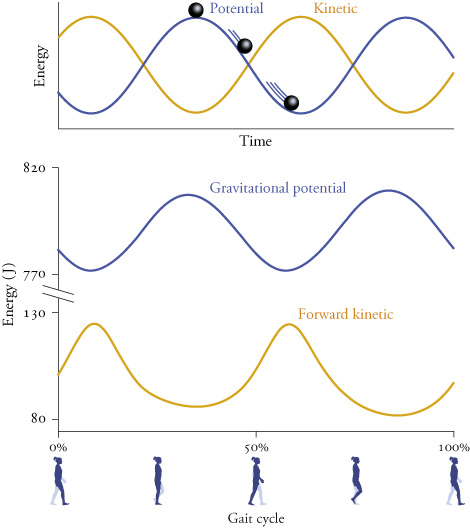
\includegraphics[width=0.8\linewidth]{chap2/2_8}
	\caption{上图:爬行动物、哺乳动物和鸟类的选定群体之间的进化关系。 
		下图:选定有胎盘的哺乳动物之间的进化关系。
		格式与图~\ref{fig:fig_2_5}~相同。
		符号(\#)表示深度分支谱系,这些谱系可以作为比较行为研究的可靠基础,以及它们的共同祖先\cite{murray2011can}。\label{fig:fig_2_8}}
\end{figure}


前额叶皮层的进化是分阶段进行的,图~\ref{fig:fig_2_8}~有助于对它们进行梳理。
一个阶段发生在早期哺乳动物身上,产生了前额叶皮层的非颗粒部分。
早期哺乳动物利用夜间觅食的生态位,新皮层在这些动物中进化出来。
非颗粒前额叶皮层与新的视觉、听觉和体感区域一起,支持了这个新生态位中的觅食选择。
第~\ref{chap:chap3}~章和第~\ref{chap:chap4}~章讨论了非颗粒前额叶皮层,表~\ref{tab:tab_4_1}~提出了一些关于它们在觅食选择中具体贡献的想法。


在前额叶皮层的后期演化中,颗粒前额叶皮层出现在早期灵长类动物身上,当它们适应了生活在树的细小树枝上的生活时,它们可以利用嫩叶、水果、花朵、花蜜和昆虫。
第一个颗粒前额叶皮层包括尾部前额叶皮层和眶上皮层的颗粒部分的同源物。
这些新的颗粒前额叶皮层当时和现在都在搜索食物和食物迹象方面发挥作用,并根据当前的生物需求评估它们的价值。
第\ref{chap:chap4}章和第\ref{chap:chap5}章涉及这些主题。


在前额叶皮层的演化的最后一个阶段发生在人猿的进化过程中。
早期的人猿从其狭鼻亚目的祖先那里继承了白天觅食和中央凹,而后来的人猿发展出了三色视觉。
随着人猿变得更大,它们在更大的家域内觅食,并依赖于特定树木的食品。
因此,它们变得容易受到这些食物的短缺的影响。
比较的证据表明,此时出现了几个新的前额叶皮层领域:
背侧前额叶皮层,腹侧前额叶皮层,以及可能还包括极端前额叶皮层。
我们提出,这些新的前额叶皮层领域在食物短缺和激烈竞争时提供了适应性优势。
在第\ref{chap:chap3}-\ref{chap:chap8}章中,我们认为这些皮层区域通过减少增加捕食风险、浪费精力或产生比其他选择更少好处的选择的频率,提高了觅食的效率。


在实验室中,浪费努力或产生较少效益的选择被称为错误。
错误的明确定义以及实验室行为和自然觅食之间的巨大差异几乎不需要提及。例如,在野外,觅食选择经常涉及哪棵树或哪个位置接近以获取食物,而在实验室中,对刺激的响应通常涉及到伸手或眼部运动以获得奖励。
觅食通常涉及物体(包括食物)的操作,但只有少数实验室测试探索了像物体操作这样复杂的动作。实验室测试有试验,但是觅食选择很少适合这样简单的时间划分。
觅食还经常涉及社交互动,实验室研究只有在最近才开始认真研究这个领域。


虽然如此,实验室实验为猕猴提供了在地点和物体之间做出选择的机会,并且这些选择会产生它们需要和消耗的食物或液体。
因此,实验室研究可以探索有助于成功觅食的认知能力。


Hayden等人\cite{hayden2011surprise}的一项开创性研究试图模拟人猿在从开发减少的资源转而探索更遥远的资源时所做的种类狩猎选择。
第~\ref{chap:chap3}~章阐述了这个实验的结果,但我们在这里提到它是因为这个任务是一个使用简单的彩色形状、变量延迟期和注视性眼动来研究人猿所做选择的例子,这些选择包括对视觉信号的响应,估计到达远程资源所需的时间以及使用四足步态行走。


因此,尽管野外觅食和控制实验室实验之间存在明显的差异,但许多有益于野外觅食的认知能力可以在实验室中进行研究。


1. 采食类灵长类动物需要将其行为与所获得的资源结果联系起来,某些实验任务可评估猕猴如何学习这种联系。
第\ref{chap:chap3}章回顾了一些研究,例如探讨了猕猴如何学习采取哪些行动以最小的努力获得最多的资源;\par


2.寻找食物的灵长类动物还需要将寻找目标(如物品)与食物结果联系起来。
它们不仅需要学习食物或液体的一般价值,还需要根据当前的需求来评估这些资源。
第\ref{chap:chap4}章回顾了一些任务,其中猕猴需要在一些与一定数量或概率的食物或液体相关联的物品之间进行选择。
其他实验可以改变反映当前生物需求的动机因素,例如允许猕猴食用某种食物以达到饱食的状态;\par


3.在自然觅食中,动物同时看到许多刺激,并将其中许多记忆。
他们需要在所有这些杂乱中找到觅食目标,并将注意力集中在它们上面,同时规划达成目标最有效的方式。
第\ref{chap:chap5}章讨论了评估注意力和搜索能力的实验任务,例如在一片绿色的正方形中挑出一个红色正方形;\par


4.灵长类动物受益于以有序和高效的方式觅食,第\ref{chap:chap6}章讨论了许多用于研究行为在时间和空间上的顺序的任务,例如学习通过视觉迷宫导航的光标或在25个不透明门中选择以获取每个门后面的单个花生。觅食还涉及将目标保留在记忆中,这个概念被称为前瞻编码。
可以使用成对联想学习任务来研究此功能,其中一个刺激表示另一个刺激应该作为目标;\par


5.当猕猴们环顾四周时,会看到一些资源的标志。
第~\ref{chap:chap7}~章讨论了条件视觉运动任务,这些任务研究标志到动作的映射。
同样的任务也可以用来研究猕猴如何使用抽象的策略。
在野外,这种能力使得类人猿能够将他们对于一般采食的学习迁移到新颖或罕见的采食问题中;\par


6.在资源不稳定的情况下,从单次经历中学习并因此限制无效或有风险的选择是很有益的。
在实验室中,这种能力导致快速学习和其他减少错误的机制。
第~\ref{chap:chap3}~和第~\ref{chap:chap8}~章回顾了探索这些功能的任务,例如选择嵌入在背景场景中的物体。


第\ref{chap:chap1}章阐述了将前额叶皮层作为一个整体进行解释的目的。
但正如本章所示,整体随着时间的推移而改变。
早期灵长类动物发展出的前额叶皮层缺乏现代人类类动物具有的许多颗粒前额叶皮层;
早期哺乳动物进化出的前额叶皮层则缺乏灵长类动物所有颗粒区域。
因此,要完全理解前额叶皮层,我们需要理解部分和整体。
为此,我们需要拆开前额叶皮层。
第~\ref{chap:chap3}~章从内侧前额叶皮层开始。


\chapter{跑步} \label{chap:chap3}

如果你能用六十秒的长跑来填补这无情的一分钟……
\begin{flushright}
	——拉迪亚德$\cdot$吉卜林
\end{flushright}


\begin{figure}[!htb]
	\centering
	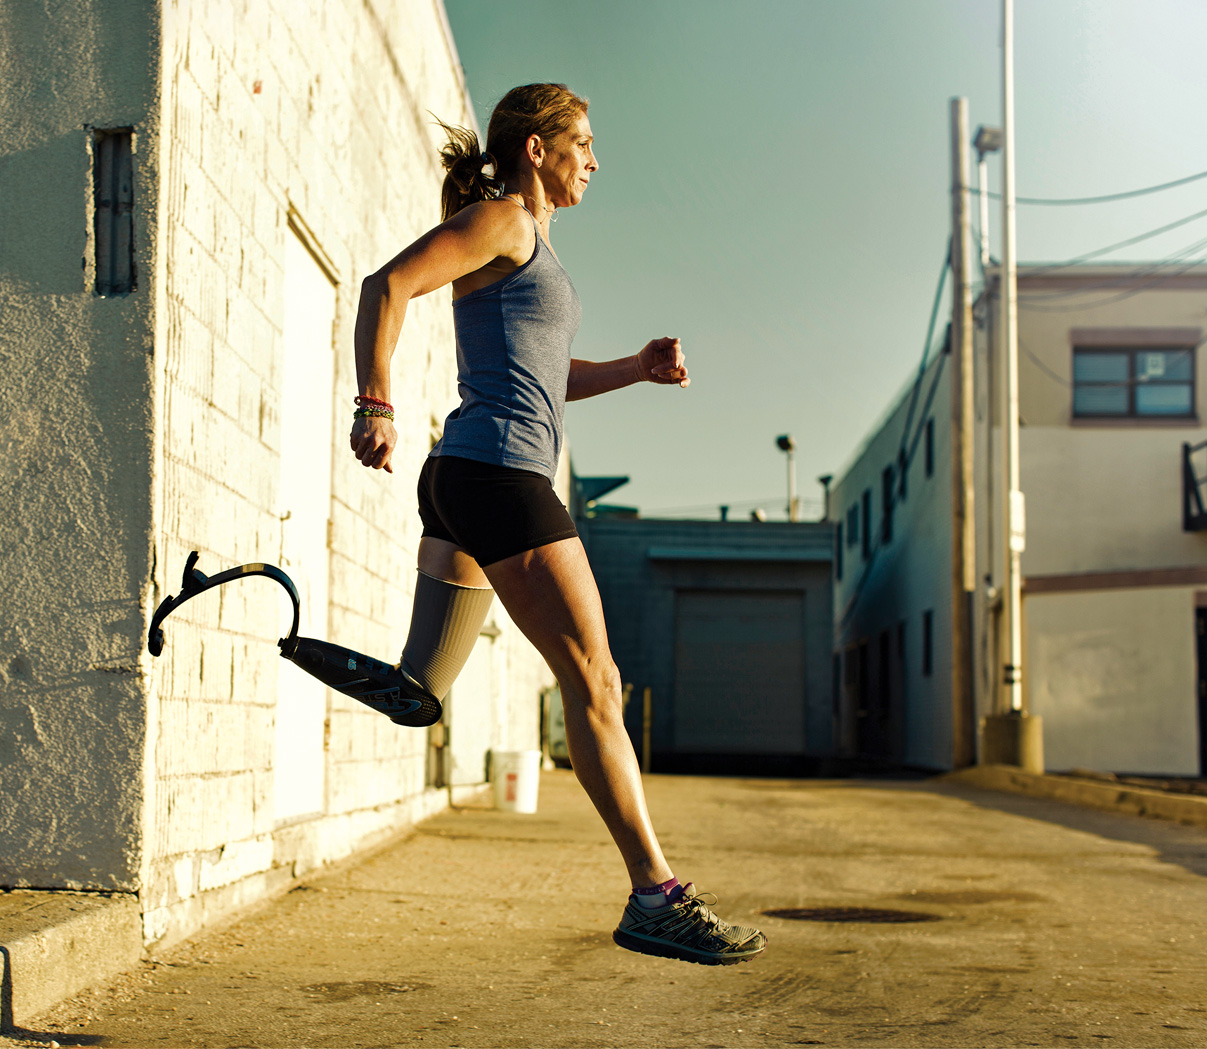
\includegraphics[width=1.0\linewidth]{chap3/3_0}
	% 加星号(*)表示不加编号
	\caption*{ \label{fig:3_0}}
\end{figure}

看过《侏罗纪公园》的人可能都记得那个标志性的场景:
一辆吉普车试图超越一只追赶的霸王龙。
有趣的是,这个场景与电影上映时(1993年)古生物学家的普遍看法相符。
当时人们认为霸王龙的奔跑速度可以达到 40 公里/小时,一些科学家甚至认为它的速度甚至可能更快。
以这样的速度,它在土路上完全可以超过一辆吉普车。


然而,自 2002 年约翰$\cdot$哈钦森(John Hutchinson)开创性论文以来,近期的生物力学研究表明,霸王龙可能根本无法奔跑。
即使它能跑,也可能无法达到 40 公里/小时的速度。
哈钦森通过模拟霸王龙,证明要达到这样的速度,其 86\% 的体重必须由腿部肌肉构成,留给其庞大的尾巴、头部和躯干的空间非常有限。
为了产生足够大的地面反作用力,它需要将如此大的质量分配给腿部肌肉,而这种反作用力在奔跑时通常超过体重的两倍。


对恐龙、大象和袋鼠等动物的研究有助于我们理清对人类跑步的理解:
是什么驱动着从步行到跑步的转变,又是什么限制了跑步速度。
地面反作用力的测量揭示了为什么跑步时比步行时更容易受伤,以及如何设计跑道来降低受伤率并提高速度。


在本章中,我们将使用简单的力学模型来探讨这些问题。
这些模型包含弹簧,用于表示肌肉和肌腱的弹性特性,并揭示弹性能量的储存和释放如何提高跑步效率。
首先,我们定义跑步步态周期,并研究其中涉及的力和弹性机制。
然后,我们将探索一些原理,帮助你设计跑道、跑鞋和假肢,从而实现快速高效的跑步。
我们还会研究从步行过渡到跑步时步态和能量消耗的变化。


\section{跑步步态周期}

跑步步态周期由单腿支撑和腾空交替的阶段组成(图~\ref{fig:3_1})。
与步行类似,一个跑步步态周期由同一条腿连续 2 次触地事件定义,其中对侧腿的触地发生在半程。
每条腿都有一个\textit{支撑期}(脚与地面接触)和一个\textit{摆动期}(脚离地)。
支撑期始于脚触地,结束于脚趾离地,在人类跑步过程中约占步态周期的 30\% 到 45\%,但在高速冲刺过程中可能只占 25\% 或更少。
回想一下,步行时支撑期的持续时间会随着步行速度的增加而缩短。
因此,随着步行速度的增加,双腿支撑的持续时间会缩短。
如果进一步提高速度,每条腿对应的支撑期最终将持续不到步态周期的一半,从而进入腾空期。


\begin{figure}[!htb]
	\centering
	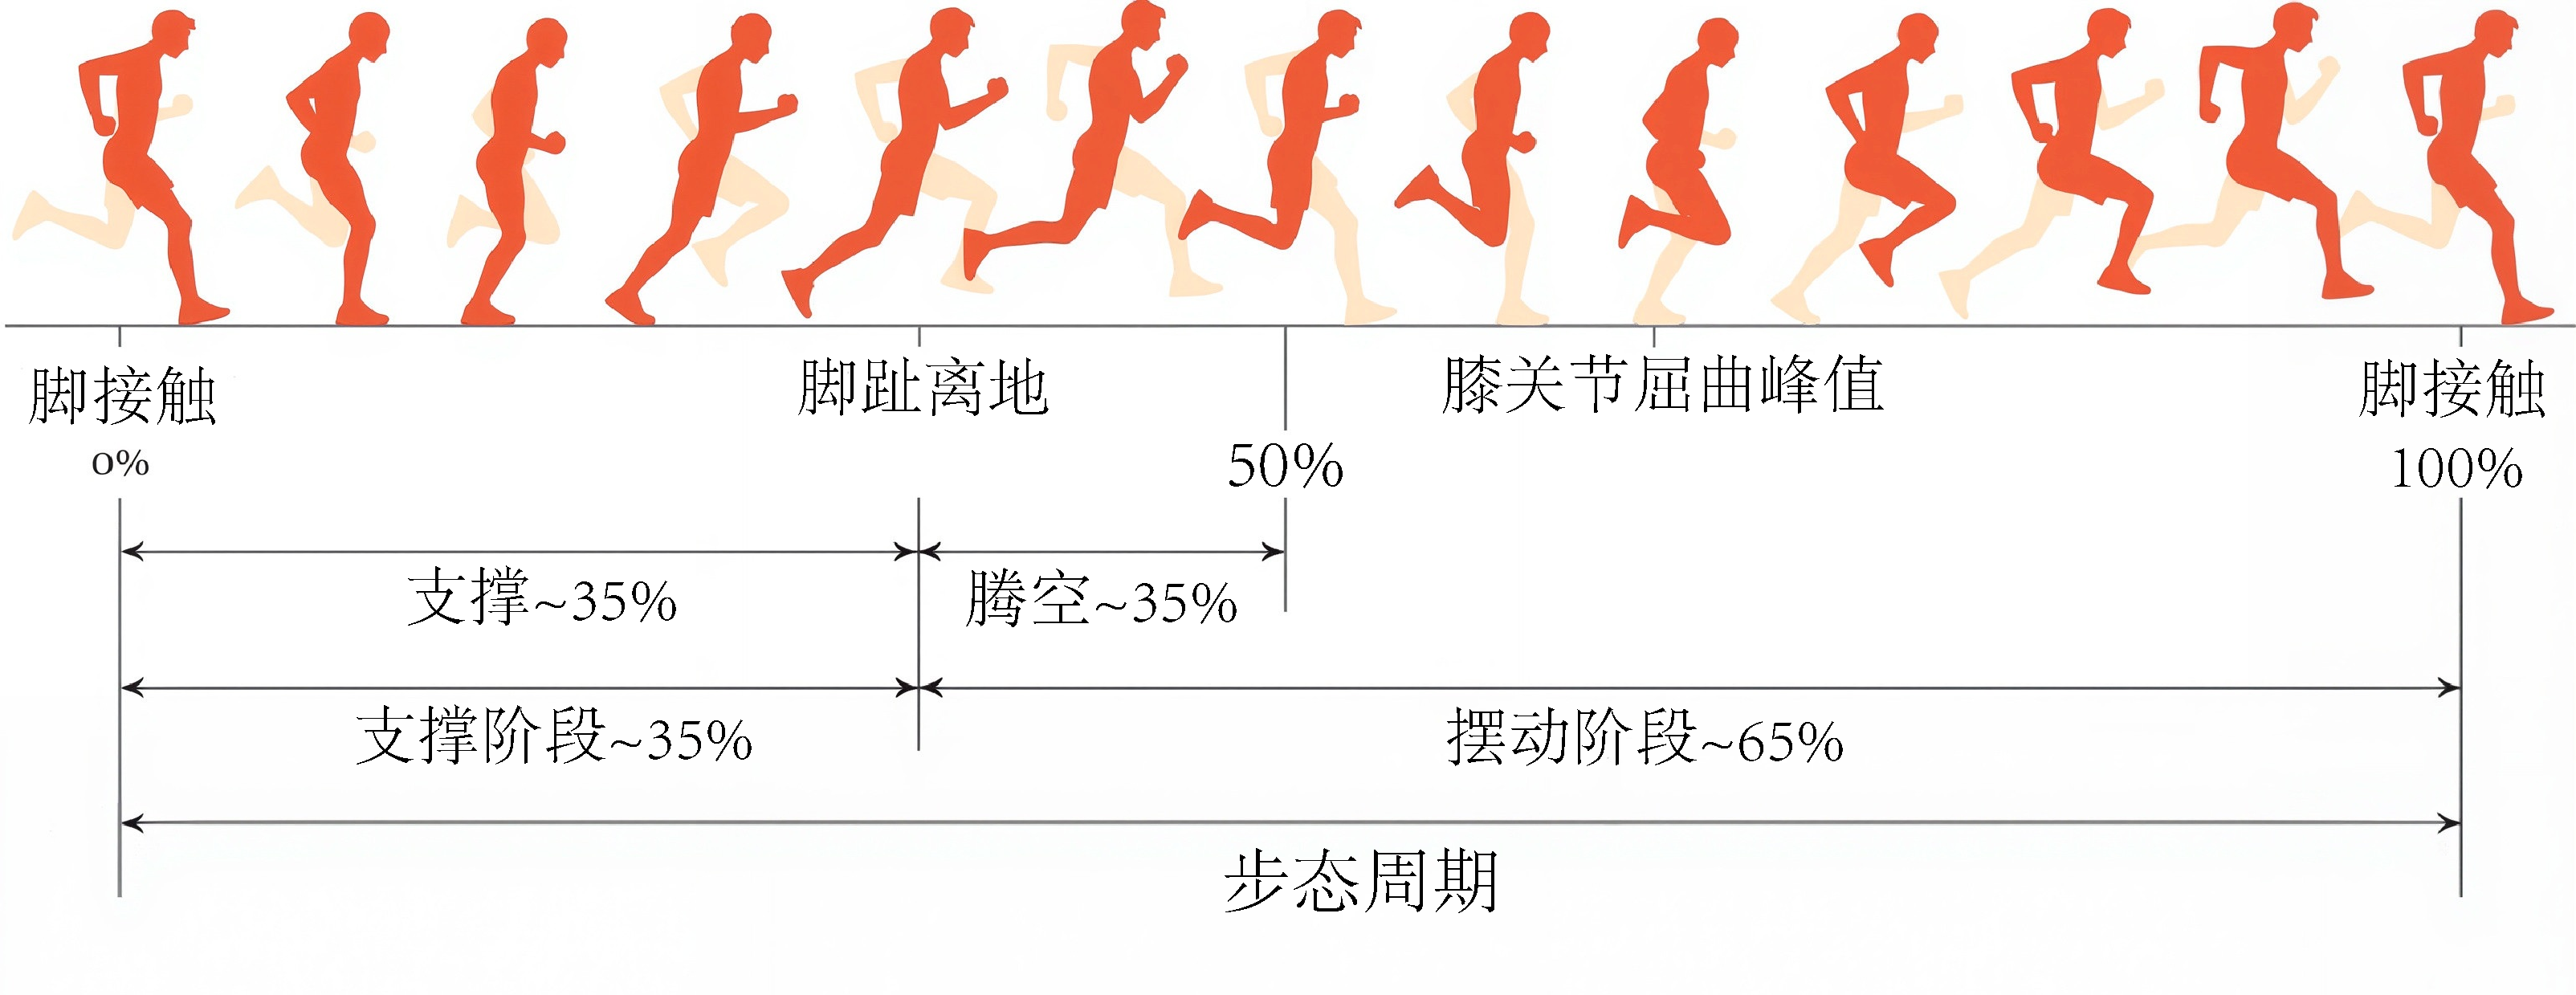
\includegraphics[width=1.0\linewidth]{chap3/3_1}
	\caption{跑步步态周期及其组成事件(例如,脚部触地)和阶段(例如,支撑)。
		站立和摆动的时间百分比会随着跑步速度和风格而变化。 \label{fig:3_1}}
\end{figure}

腾空阶段的存在是我们区分行走和跑步的一个方式。
事实上,人们很容易相信它是跑步的特征,不仅对人类如此,对其他动物也是如此。
然而,我们很快就会看到,当我们从行走步态转换为跑步步态时,会发生另一种质的变化,从生物力学的角度来看,这一点更为重要。


用于量化跑步步态周期的指标与用于步行的指标类似。
步长是两个连续足迹之间沿行进线的距离。
连续两步所走的距离,或一个步态周期所走过的距离,称为步长。
足部接触事件发生的速率(相当于步长持续时间的倒数)称为步频;
迈步的速率称为步频。
跑步速度可以用步长与步频的乘积来计算,
或者,也可以用步长与步频的乘积来计算:

\begin{equation}
	\text{速度(米/秒)} = \text{步长(米/步)} \times \text{节律(步/秒)} \label{eq:3_1}
\end{equation}

中等跑步速度为 4 米/秒。
在此速度下,支撑期约占步态周期的 35\% 至 40\%,典型的步频为 180 步/分钟,典型的步长约为 1.3 至 1.4 米:

\begin{equation}
	\text{步长} = \frac{4.0 \text{米}}{1 \text{秒}}
				 \times \frac{60 \text{秒}}{1 \text{分钟}}
				 \times \frac{1 \text{分钟}}{180 \text{步}}
				 = 1.33 \text{米/秒}
				 \label{eq:3_2}
\end{equation}

当然,这些数量会随着腿长、跑步风格、鞋类和其他因素而变化。













\part{移动的产生}
\markboth{移动产生}{移动的产生}

\chapter{肌肉生物学和肌肉力量}\label{chap:chap4}


孤身一人,我们能做的太少。
团结起来,我们能做的却很多。
\begin{flushright}
	————海伦$\cdot$凯勒
\end{flushright}


\begin{figure}[!htb]
	\centering
	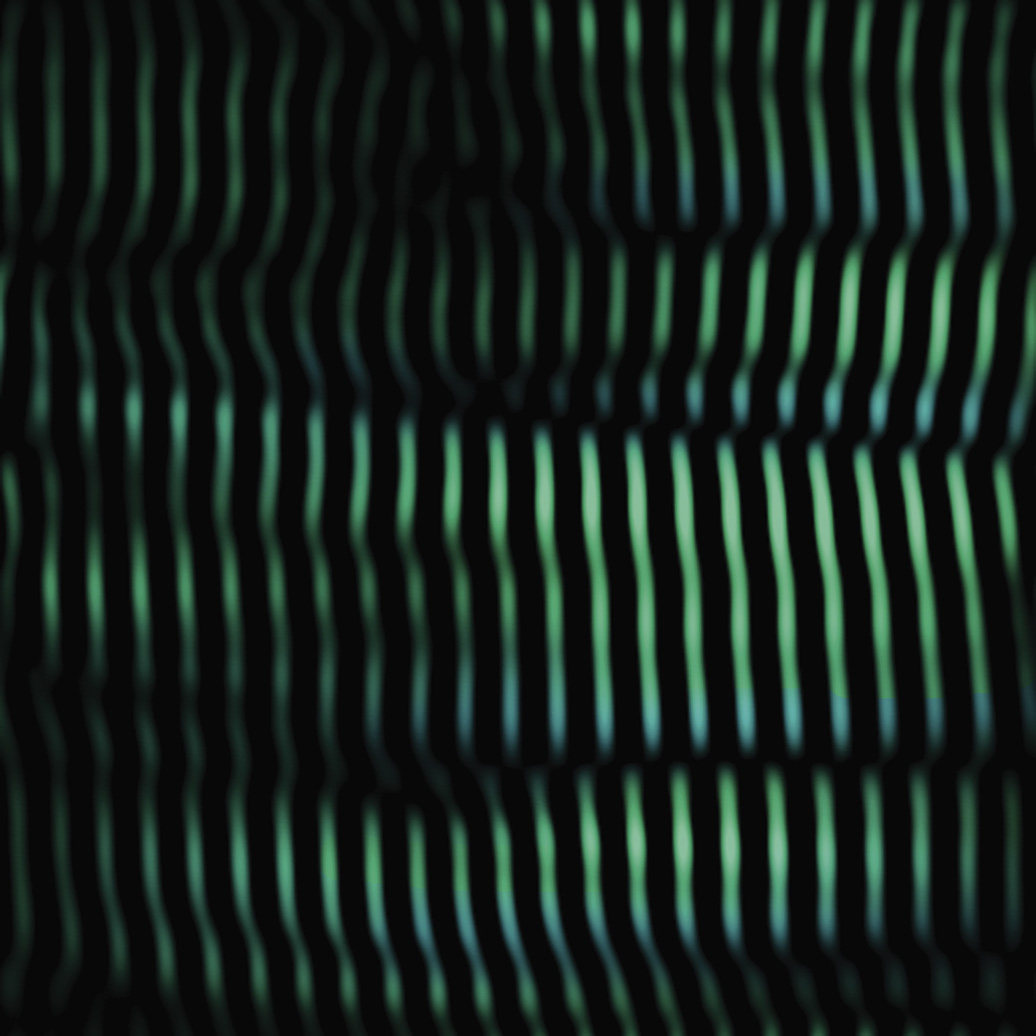
\includegraphics[width=1.0\linewidth]{chap4/4_0}
	% 加星号(*)表示不加编号
	\caption*{ \label{fig:4_0}}
\end{figure}


伦敦皇家学会拥有 350 年的历史,拥有近 200 年的传统,每年都会邀请科学家进行公开演讲,并经常进行一些简单的实验。
1952 年,其中一项实验成为了热议话题。


两辆固定自行车朝向相反,并通过一条链条连接在一起,当一辆自行车向前踩踏板时,另一辆自行车的踏板就会向后移动(图~\ref{fig:4_1})。


\begin{figure}[!htb]
	\centering
	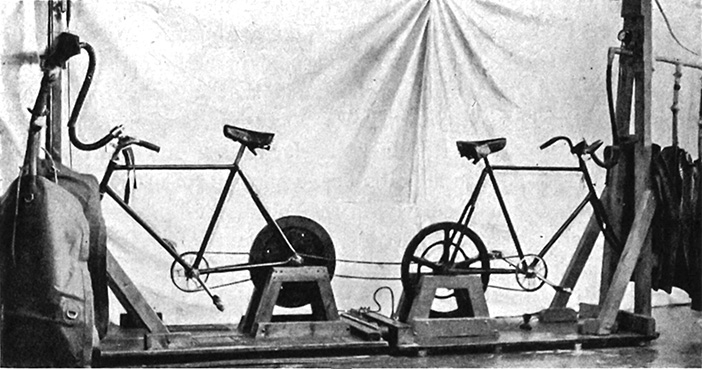
\includegraphics[width=1.0\linewidth]{chap4/4_1}
	\caption{\textit{艾博特}等人描述的推拉装置\cite{abbott1952physiological}。 \label{fig:4_1}}
\end{figure}


一辆自行车上坐着一位娇小的女子,名叫布伦达$\cdot$比格兰,是肌肉疲劳研究领域的权威专家。
另一辆自行车上坐着一位魁梧的年轻人,名叫默多克$\cdot$里奇,他嫁给了他的自行车“对手”。
演讲者是A$\cdot$V$\cdot$希尔,他因在肌肉产热方面的研究而获得了诺贝尔奖。


里奇听从指令,用尽全力向前蹬,而比格兰则用力蹬着脚蹬,阻止他继续蹬。
想象一下,当观众看到这位娇小的女子轻而易举地阻止了这位身材高大的男人蹬得更快时,他们会有多么惊讶。
很快,他便大汗淋漓,气喘吁吁,而比格兰却几乎毫不费力。
甚至连伦敦市长后来也过来试驾。
“这套设备后来被命名为‘推拉你’,以纪念杜立特医生那只永远不知道自己要往哪个方向跑的双头怪兽,”布伦达$\cdot$比格兰-里奇后来写道。


魔术?小把戏?
并非如此,但它确实表明,肌肉消耗能量和产生力量的方式并非显而易见。
肌肉做正功(例如,在向前蹬踏时充当“马达”)时,它们消耗的能量和产生的热量,比做负功(例如,在向前蹬踏时充当“刹车”)时要多。
一般来说,肌肉产生的力量和消耗的能量,很大程度上取决于它是缩短还是伸长。
希尔实验的经验教训至今仍在日常康复和阻力训练中得到应用。
正如我们将看到的,奇迹发生在分子层面。


本章和下一章将深入探究肌肉内部,探索其结构与功能之间的关系。
肌肉是神奇的生物马达,能够在瞬间悄无声息地产生数千牛顿的力量。
这些力量如此巨大,以至于你小腿的肌肉就能举起一辆小型汽车的尾部。
这些巨大的力量是由数万亿个纳米级分子马达共同作用产生的,这些马达将我们摄入食物中的化学能转化为机械能,使我们能够活动。
这一非凡的功能源于骨骼肌特化的细胞机制和高度组织化的层级结构(图~\ref{fig:4_2})。


\begin{figure}[!htb]
	\centering
	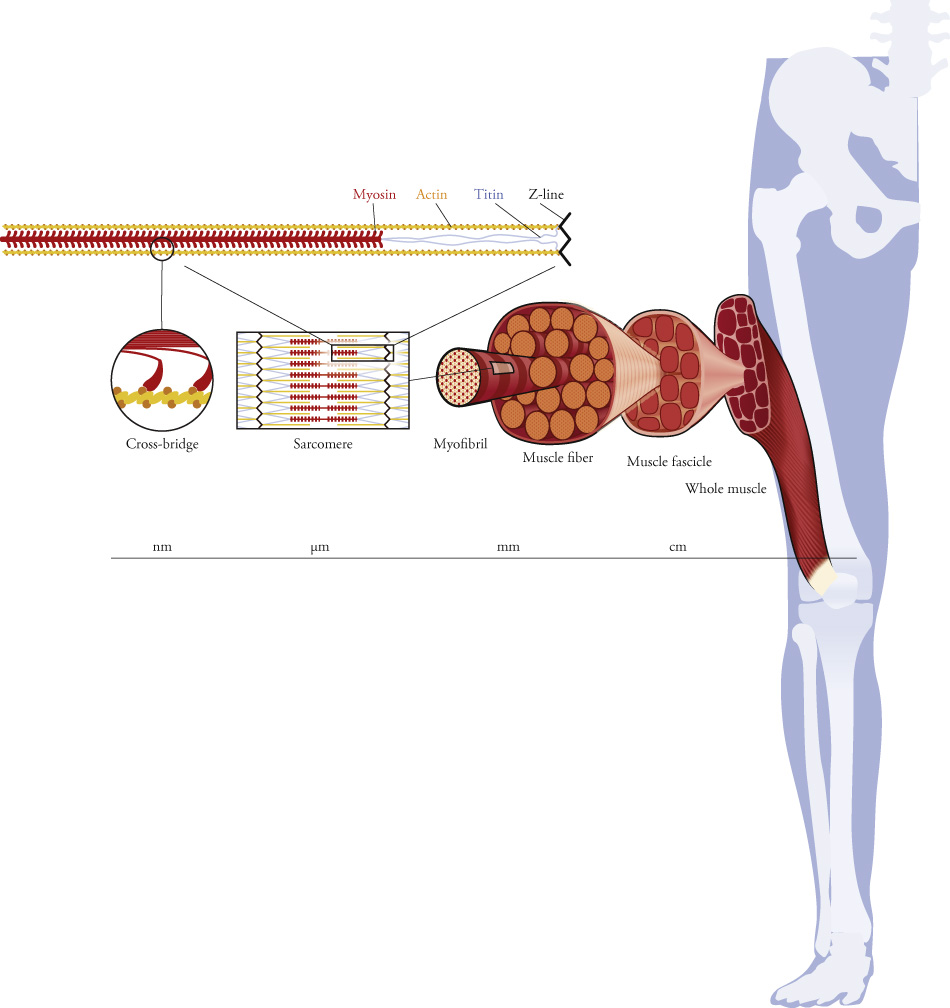
\includegraphics[width=1.0\linewidth]{chap4/4_2}
	\caption{肌肉的多尺度结构。
		骨骼肌具有层次结构,其中有被称为\textit{肌球蛋白}的纳米级分子马达,每个肌球蛋白仅产生几皮牛顿的力,排列成肌节、肌原纤维、纤维、肌束和整个肌肉,在强力肌肉收缩期间可产生数千牛顿的力。 \label{fig:4_2}}
\end{figure}


接下来两章的组织将大致遵循肌肉的层级结构。
我们将首先在分子层面研究力量的产生过程。
接下来,我们将了解分子马达是如何被包裹在被称为肌节的亚细胞结构中的(活体人体肌节的第一张图像就是在我的手臂上拍摄的,并在本章的开篇图中展示)。
进一步深入,我们将了解单个肌肉细胞如何被神经系统激活,并了解“快肌纤维”和“慢肌纤维”之间的区别。
在第~\ref{chap:chap5}~章中,我们将从宏观层面研究肌肉在体内的排列方式,以及它们如何与肌腱(将肌肉力量传递到骨骼结构)相互作用。


\section{肌肉结构}

从最基本的层面来说,肌肉通过两种细长蛋白质(肌动蛋白和肌球蛋白)的相互作用产生力量。
20 世纪 50 年代初,休$\cdot$赫胥黎通过 X 射线显微镜发现,这些蛋白质平行排列,纤维交织,它们之间的连接被他称为“横桥”。
安德鲁$\cdot$赫胥黎(与休无亲属)同时用不同的方法发现了横桥。
休$\cdot$赫胥黎和安德鲁$\cdot$赫胥黎都怀疑横桥是产生力量的机制,并于 1954 年提出了一个关于这些分子马达如何工作的模型,我们将在下文中解释。
他们的模型一直是解释力量产生的基本范式,尽管随着更多实验数据的收集,该模型变得更加详细。


从尺寸上看,肌纤维排列成束,称为肌束,它们与肌肉纤维一样,长度可达数十厘米。
肌束的横截面积约为 1 毫米。
除了肌纤维外,肌束还包含称为细胞外基质的结缔组织,其中包括胶原蛋白、神经纤维和血管。
在健康的肌肉中,肌纤维紧密排列;
然而,在患病的肌肉中,肌纤维的横截面积可能较小,并被更多的细胞外基质和脂肪隔开。


肌束被更多结缔组织包围,并聚集在一起形成肌肉。
另一层结缔组织鞘被称为筋膜,包裹着肌肉并将其与其他肌肉隔开。
终止于每个肌束末端的肌纤维可以直接附着在骨骼上,但通常它们会连接到肌腱,肌腱随后附着在骨骼上。
肌腱插入肌肉的部分称为腱膜;
肌腱在肌肉外部的部分通常称为游离肌腱。
正如我们将在第~\ref{chap:chap5}~章中看到的,肌腱不仅通过向骨骼传递肌肉力量发挥着重要作用,还在伸展和回缩时储存和释放能量。


\section{横桥循环}

当神经系统激活肌肉时,肌肉会通过数万亿个\textcolor[RGB]{226,128,39}{肌动蛋白}和\textcolor[RGB]{198,9,5}{肌球蛋白}的协同作用产生力量,这个过程被称为\textit{横桥循环}(图~\ref{fig:4_3})。
这种机制可以粗略地描述为一个分子大小的(防止倒转的)棘齿。


\begin{figure}[!htb]
	\centering
	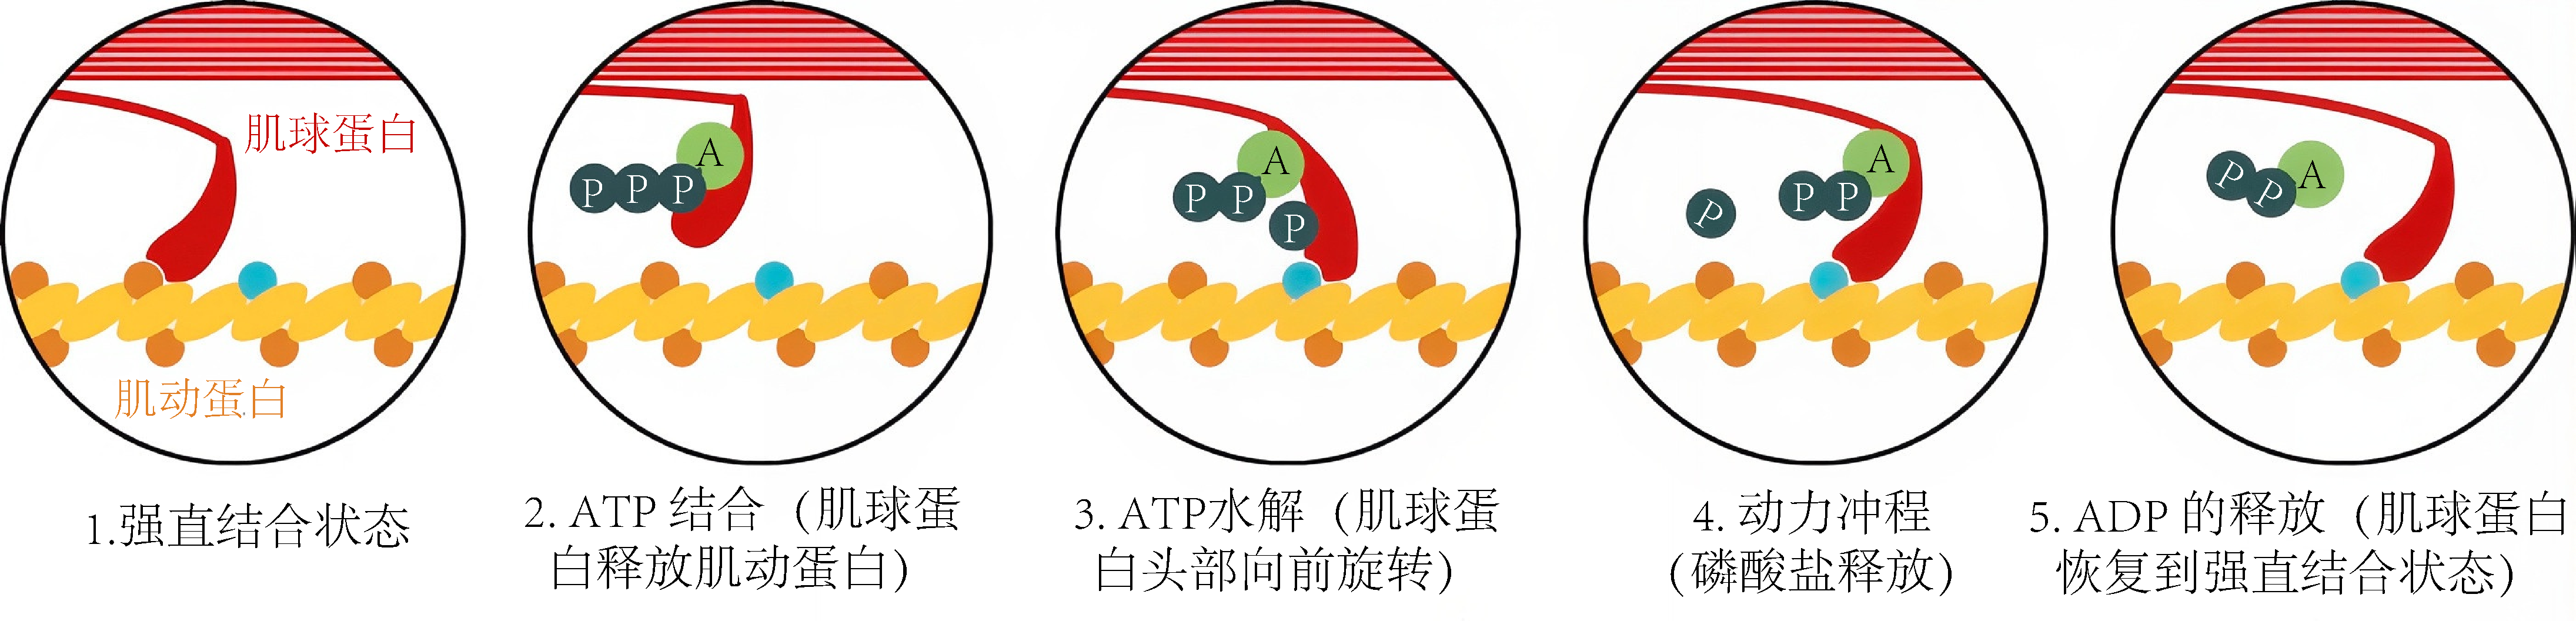
\includegraphics[width=1.0\linewidth]{chap4/4_3}
	\caption{横桥循环描述了\textcolor[RGB]{226,128,39}{肌动蛋白}和\textcolor[RGB]{198,9,5}{肌球蛋白}相互作用产生力量和运动的过程。
		A 代表\textit{腺苷};P 代表\textit{磷酸}。 \label{fig:4_3}}
\end{figure}

如图~\ref{fig:4_4}~的顶部,肌球蛋白分子分为 3 个区域,分别称为\textit{头部}、\textit{颈部}和\textit{尾部}。
\textcolor[RGB]{198,9,5}{肌球蛋白}头部的独特结构使其能够牢固地结合到\textcolor[RGB]{226,128,39}{肌动蛋白}丝上的特定位置(图~\ref{fig:4_3}~中的第一帧)。
当肌肉需要产生力量时,\textcolor[RGB]{198,9,5}{肌球蛋白}头部会接收一种名为三磷酸腺苷 (adenosine triphosphate, ATP) 的“燃料”分子。
这刺激\textcolor[RGB]{198,9,5}{肌球蛋白}头部从\textcolor[RGB]{226,128,39}{肌动蛋白}上分离,向前旋转,并附着到肌动蛋白上的下一个结合位点(图~\ref{fig:4_3}~中的第二帧和第三帧)。
接下来,\textcolor[RGB]{198,9,5}{肌球蛋白}头部围绕颈部区域旋转,这一运动被称为\textit{动力冲程},产生几皮牛的力,并使肌动蛋白丝彼此滑动约 10 纳米。


当然,不消耗能量就不可能完成机械功。
能量来自于一个化学反应,该反应将一个\textit{磷酸}离子从\textit{三磷酸腺苷}中分离出来(图~\ref{fig:4_3}~中的图4),留下\textit{二磷酸腺苷}。
最终,二磷酸腺苷被释放,肌球蛋白恢复到其原始状态,但现在已从其原始位置移位。
当\textcolor[RGB]{198,9,5}{肌球蛋白}以这种方式循环时,细丝被拉向肌节中部,从而在化学能转化为机械能的过程中产生张力。


虽然这种机制听起来可能很复杂,但它却是一个优雅而经济的解决方案,解决了如何在分子层面上以可预测的方向产生力的问题。
就像汽车发动机一样,我们的肌肉将化学能转化为机械能,但噪音更小,产生的有毒废气也更少。



\section{肌节结构}

再往上一层,我们来看看肌节。
肌节大致呈圆柱形,长度根据肌肉长度在 1 微米到 5 微米之间变化。
肌节由许多相互交织的“粗”肌丝和“细”肌丝组成,随着肌节长度的变化,这些肌丝会相互滑动。


数百条肌球蛋白尾部捆绑在一起,形成每根粗肌丝,形成棒状结构,肌球蛋白头部以规则的间隔向外放射状延伸(图~\ref{fig:4_4})。
与粗肌丝平行的是细肌丝,它们由 3 种蛋白质组成:
肌动蛋白、原肌球蛋白和肌钙蛋白。
我们已经描述了肌动蛋白,它为肌球蛋白头部提供结合位点。
这些结合位点沿着细肌丝以规则的间隔分布。
原肌球蛋白和肌钙蛋白仅在肌肉被神经系统激活且存在钙离子时才会暴露这些结合位点,从而帮助调节力量的产生。
另一种值得关注的蛋白质(肌联蛋白),将每根粗肌丝附着在肌节的末端(我们称之为 Z 线或 Z 盘)。
正如我们稍后将看到的,肌联蛋白在被动力的产生中起着重要作用,这是一个独立于横桥循环的过程,也是赫胥黎最初的模型所忽略的现象。

\begin{figure}[!htb]
	\centering
	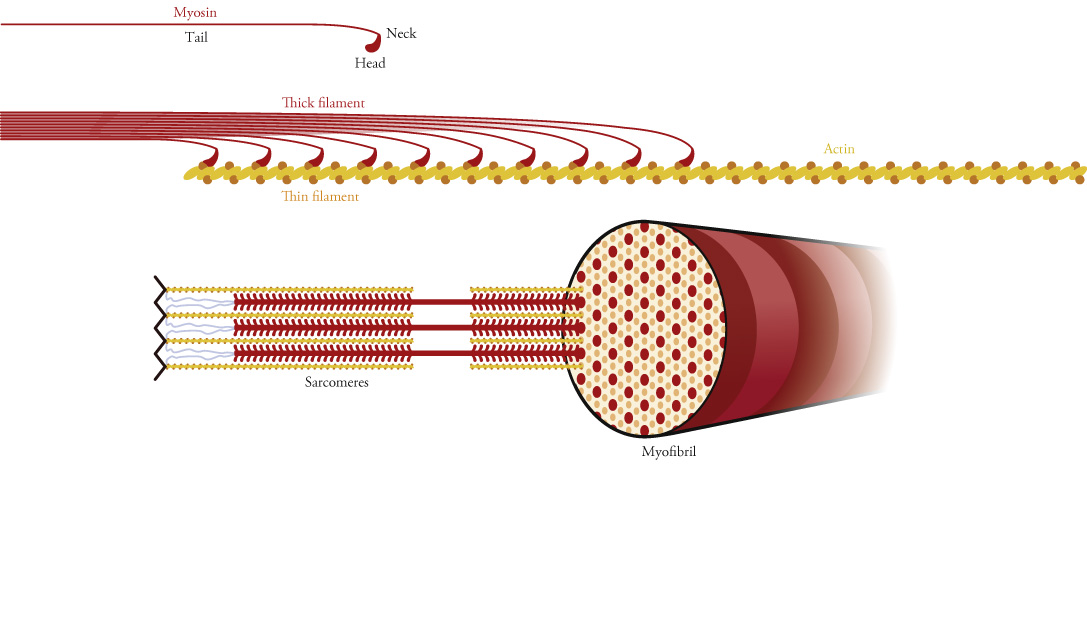
\includegraphics[width=1.0\linewidth]{chap4/4_4}
	\caption{\textcolor[RGB]{198,9,5}{肌球蛋白}示意图(顶部)、\textcolor[RGB]{186,26,26}{粗肌丝}和\textcolor[RGB]{218,128,42}{细肌丝}的相互作用示意图(中间)以及\textit{肌原纤维}横截面,显示\textcolor[RGB]{186,26,26}{粗肌丝}和\textcolor[RGB]{218,128,42}{细肌丝}以高度有序的三维模式排列(底部)。 \label{fig:4_4}}
\end{figure}

肌节在骨骼肌内以规则的模式串联和平行排列,在显微镜下观察骨骼肌组织时,会形成条纹,即明暗交替的带状结构。
您可以在图~\ref{fig:4_5}~中看到这些带状结构,它们分别被称为 I 带、A 带、Z 盘和 M 盘。
严格来说,Z 盘和 M 盘确实是圆盘,但它们通常被称为 Z 线和 M 线,因为它们在二维空间中看起来是这样的。
A 带仅出现在含有肌球蛋白的区域,而 I 带则出现在其他区域。细肌动蛋白丝的一端锚定在 Z 盘上。
粗肌球蛋白丝的一端附着在 M 盘的结构上,另一端通过肌联蛋白分子固定在 Z 盘上。
骨骼肌有时被称为“横纹肌”,与“平滑肌”相对,例如控制血管口径的肌肉,它们没有组织成肌节,也没有呈现条纹图案。

\begin{figure}[!htb]
	\centering
	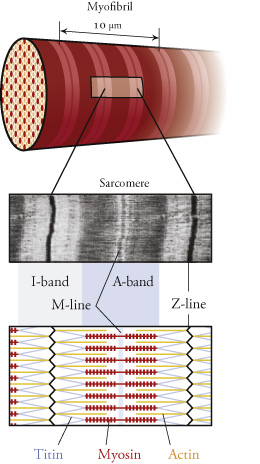
\includegraphics[width=0.5\linewidth]{chap4/4_5}
	\caption{\textit{肌原纤维}示意图(上)展示了其高度组织化的微观结构。
		肌肉显微镜图像(中)和\textit{肌节}示意图(下)分别标记了 I 带、A 带、M 线和 Z 线。
		肌节的末端由 Z 线定义。 \label{fig:4_5}}
\end{figure}


\section{力-长度关系}

肌节所能产生的最大力量会随着其长度的变化而变化。
长度和张力之间的关系可以用滑动丝理论来解释,该理论由两个研究小组于 1954 年独立提出。
Andrew Huxley 和 Rolf Niedergerke(在单根肌纤维中)以及 Hugh Huxley 和 Jean Hanson(在分离的肌原纤维中)证明,在主动肌肉收缩过程中,肌小节带不会变窄,这推翻了粗肌丝缩短的流行理论。
他们给出的解释是,随着肌节长度的变化,粗肌丝和细肌丝会相互滑动。
因此,肌节的长度会影响肌动蛋白和肌球蛋白之间“重叠”的量,或者说靠近细肌丝上结合位点的肌球蛋白头部的数量。
随着肌球蛋白头部和肌动蛋白结合位点之间横桥数量的增加,激活的肌节内的张力也会增加。


如图~\ref{fig:4_6}~所示,激活的肌肉中横桥循环所能产生的力随肌节长度而变化。
该主动力-长度曲线通常被描述为具有 3 个区域:
上升区,其中力随肌节长度的增加而增加;
平台区,其中力保持在最大值;
下降区,其中力随肌节长度的增加而减小。
平台区涵盖一系列肌节长度,称为“最佳”范围,其中肌球蛋白头部和肌动蛋白结合位点之间的相互作用数量达到最大值。
最佳肌节长度因脊椎动物而异,但通常在 2.2 至 2.7 微米之间,在人类骨骼肌中约为 2.7 微米。
当肌节长度超过最佳范围时,肌动蛋白和肌球蛋白的重叠量会减少,横桥循环所能产生的力量也会减少。
当肌节长度略短于最佳长度时,源自肌节两端的细肌丝开始在肌节中部重叠并相互干扰,导致所谓的“浅上升区”的力量减弱。
当肌节长度更短时(在“陡峭上升区”),粗肌丝会与Z盘碰撞并变形,产生阻碍横桥循环作用的力量。
由于肌肉由串联和并联排列的肌节组成,我们可以观察到肌肉主动收缩过程中力量与长度之间的类似关系。

\begin{figure}[!htb]
	\centering
	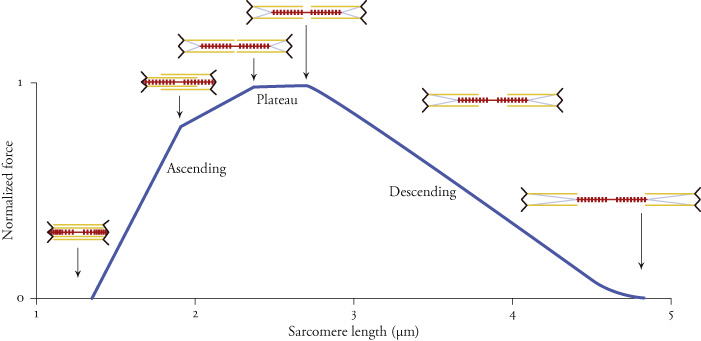
\includegraphics[width=0.9\linewidth]{chap4/4_6}
	\caption{\textit{肌节}产生的主动力与其\textit{长度}有关。
		粗肌丝和细肌丝相互滑过时,力会发生变化。
		在肌节的上升部分,力随长度增加而增大,达到平台期;
		在肌节的下降部分,力随长度增加而减小。
		当横桥数量达到最大时,力的产生达到峰值\cite{gordon1966variation}。 \label{fig:4_6}}
\end{figure}


即使在不活动时,肌肉在拉伸超过其静息长度时也会产生力,就像非线性弹簧一样。
这种被动力-长度关系主要源于肌肉中的两种结构:肌联蛋白以及围绕纤维、肌束和肌肉的结缔组织。
肌联蛋白是一种大型、柔韧的蛋白质,它将粗肌丝固定在肌节两端的Z形盘上。
当肌节较短时,肌联蛋白呈卷曲状,刚度较低;随着肌节变长,肌联蛋白变直,刚度增加(图~\ref{fig:4_7})。
肌纤维周围的结缔组织也表现出类似的力-长度行为。肌肉激活时产生的总力是其被动力与横桥产生的主动力之和(图~\ref{fig:4_8})。

\begin{figure}[!htb]
	\centering
	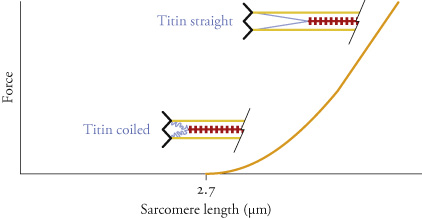
\includegraphics[width=0.7\linewidth]{chap4/4_7}
	\caption{\textit{肌联蛋白}将粗肌丝附着在肌节两端的 Z 盘上,并在拉伸时产生力量。 \label{fig:4_7}}
\end{figure}

\begin{figure}[!htb]
	\centering
	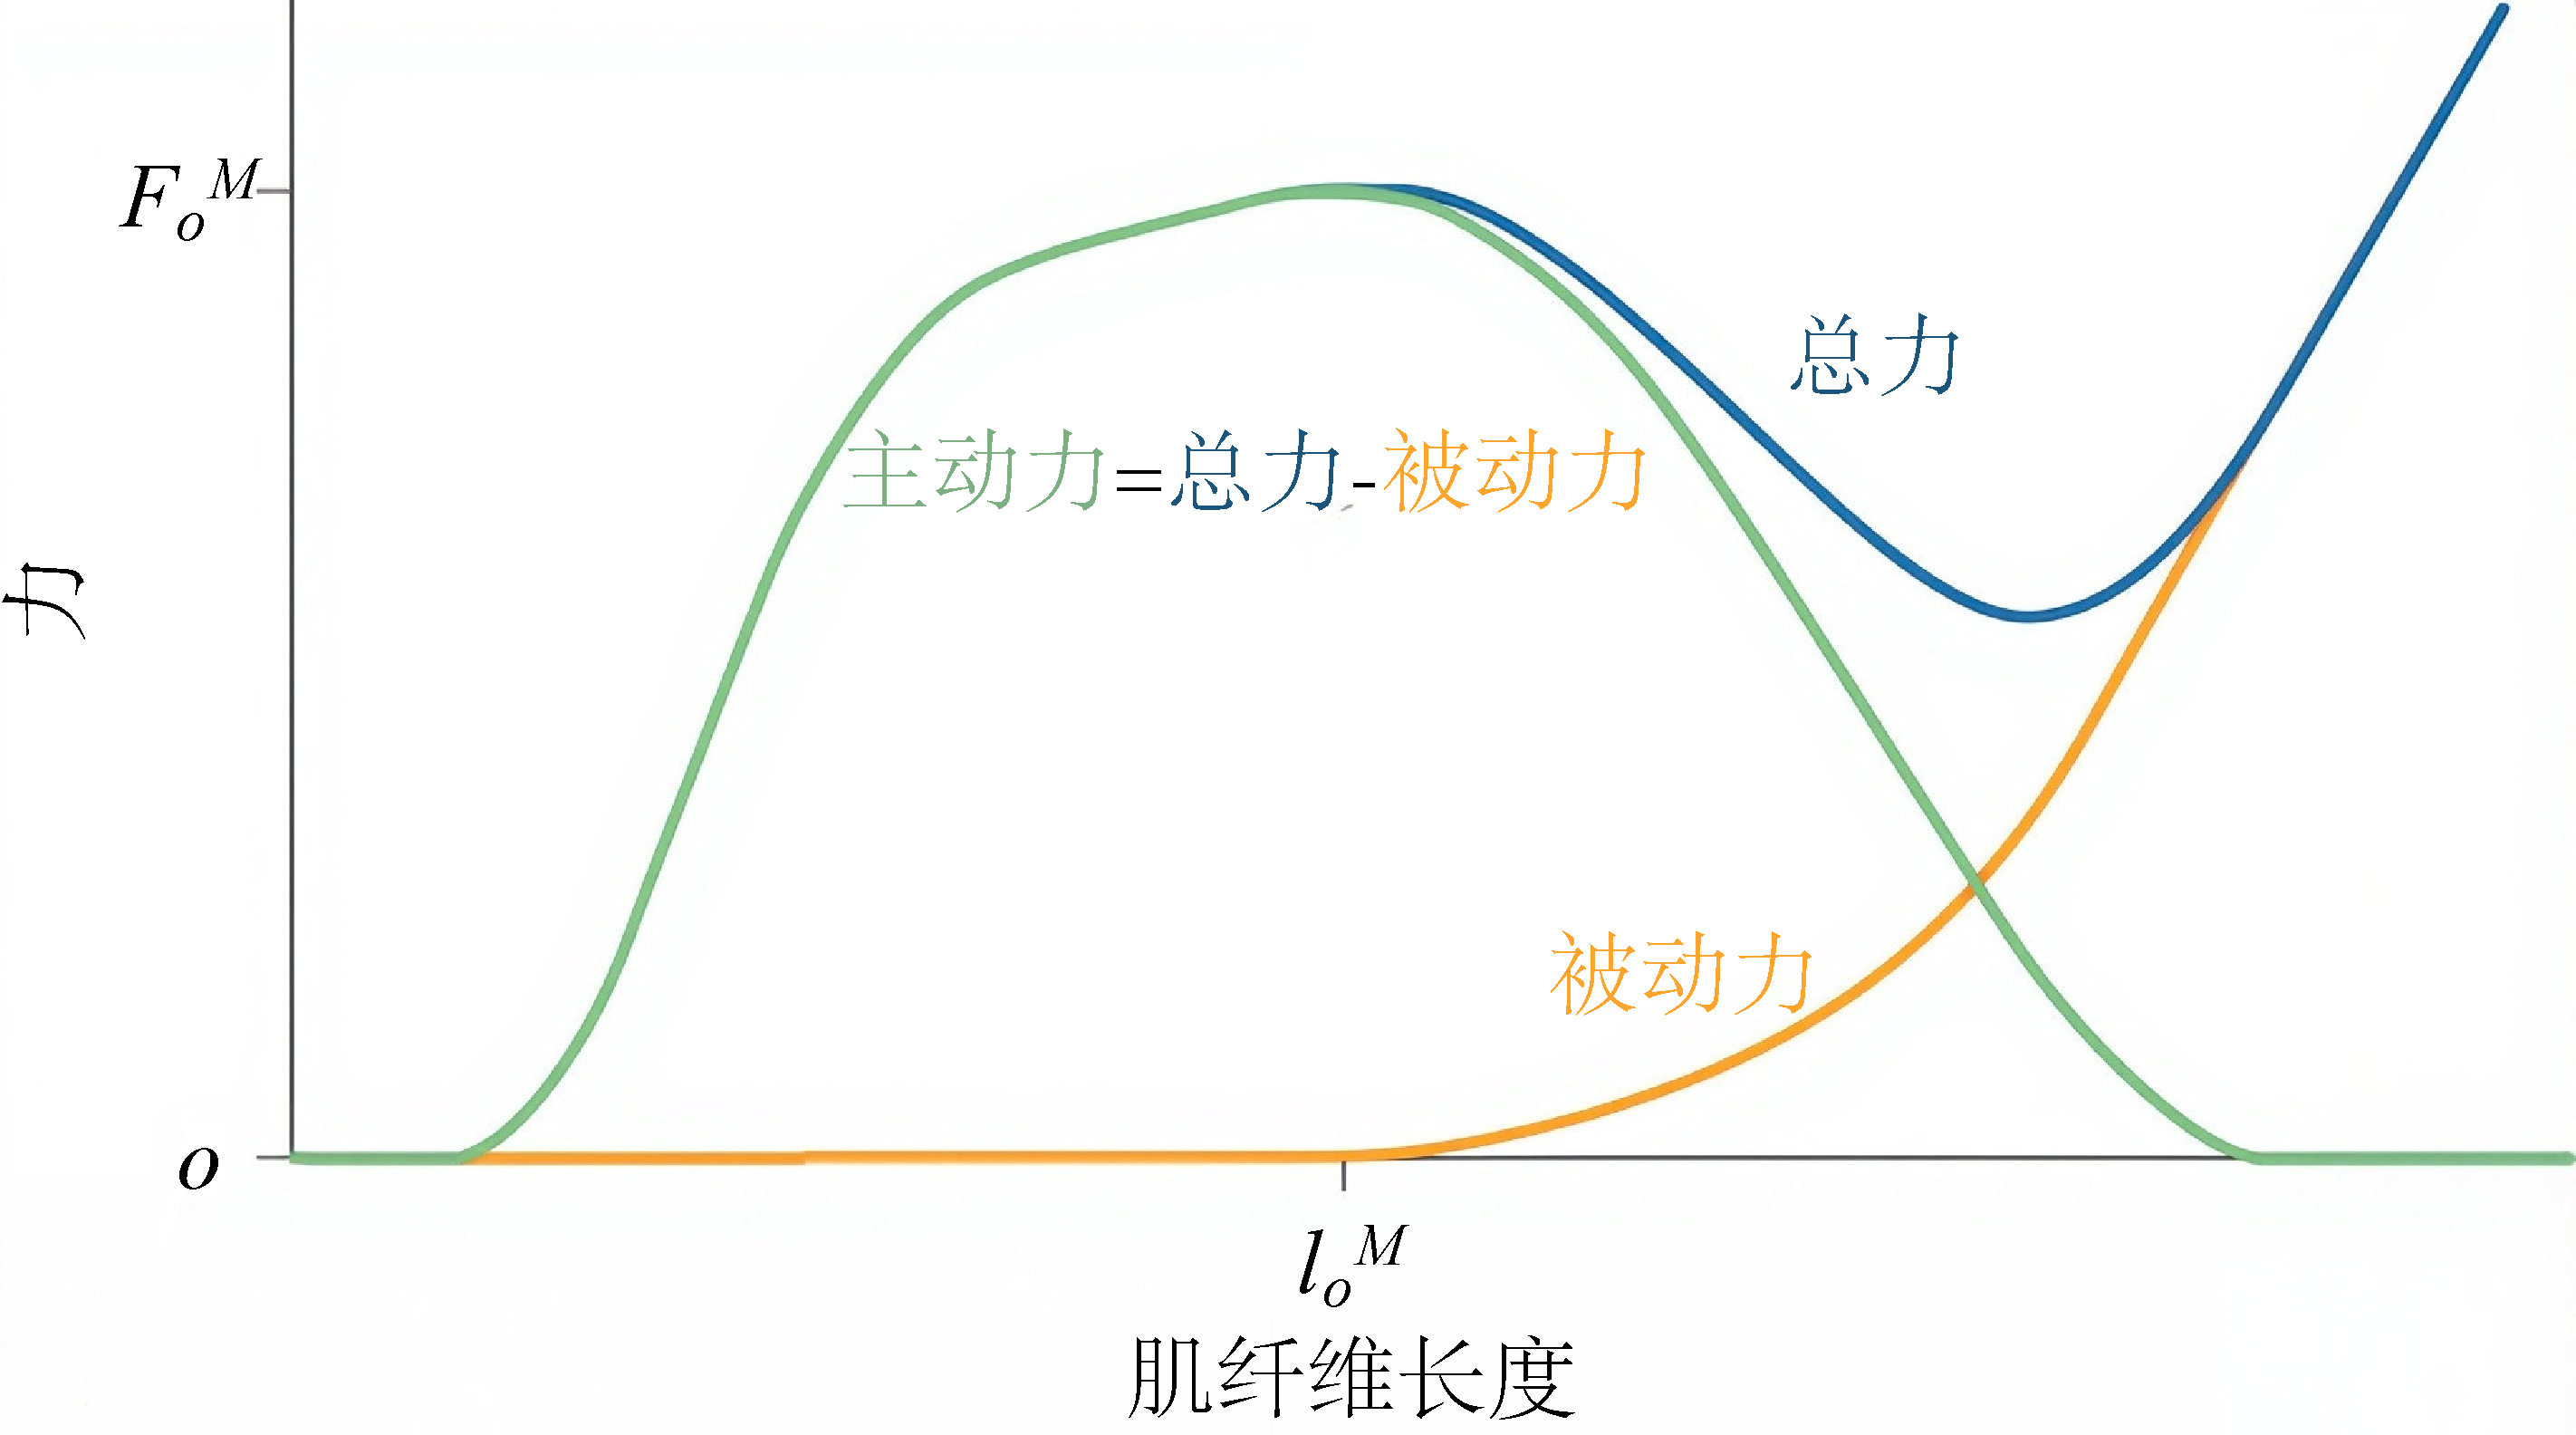
\includegraphics[width=0.7\linewidth]{chap4/4_8}
	\caption{\textcolor[RGB]{124,176,128}{主动力}-长度曲线可以通过从一系列纤维长度的\textcolor[RGB]{27,85,123}{总力}中减去\textcolor[RGB]{255,165,45}{被动力}的测量值来确定。
		峰值主动力 $F_o^M$ 出现在最佳肌纤维长度 $l_o^M$ 处。 \label{fig:4_8}}
\end{figure}


\section{力与速度的关系}

肌肉产生的力量不仅取决于其长度,还取决于其长度变化的速率,这一点可能会让人感到惊讶。
我们用力-速度曲线(图~\ref{fig:4_9})来描述这种速率依赖性。
这种关系最早由A. V. Hill于1938年观察到,并最终促使他和他的同事们开发了本章开头描述的“推我拉你”实验。

\begin{figure}[!htb]
	\centering
	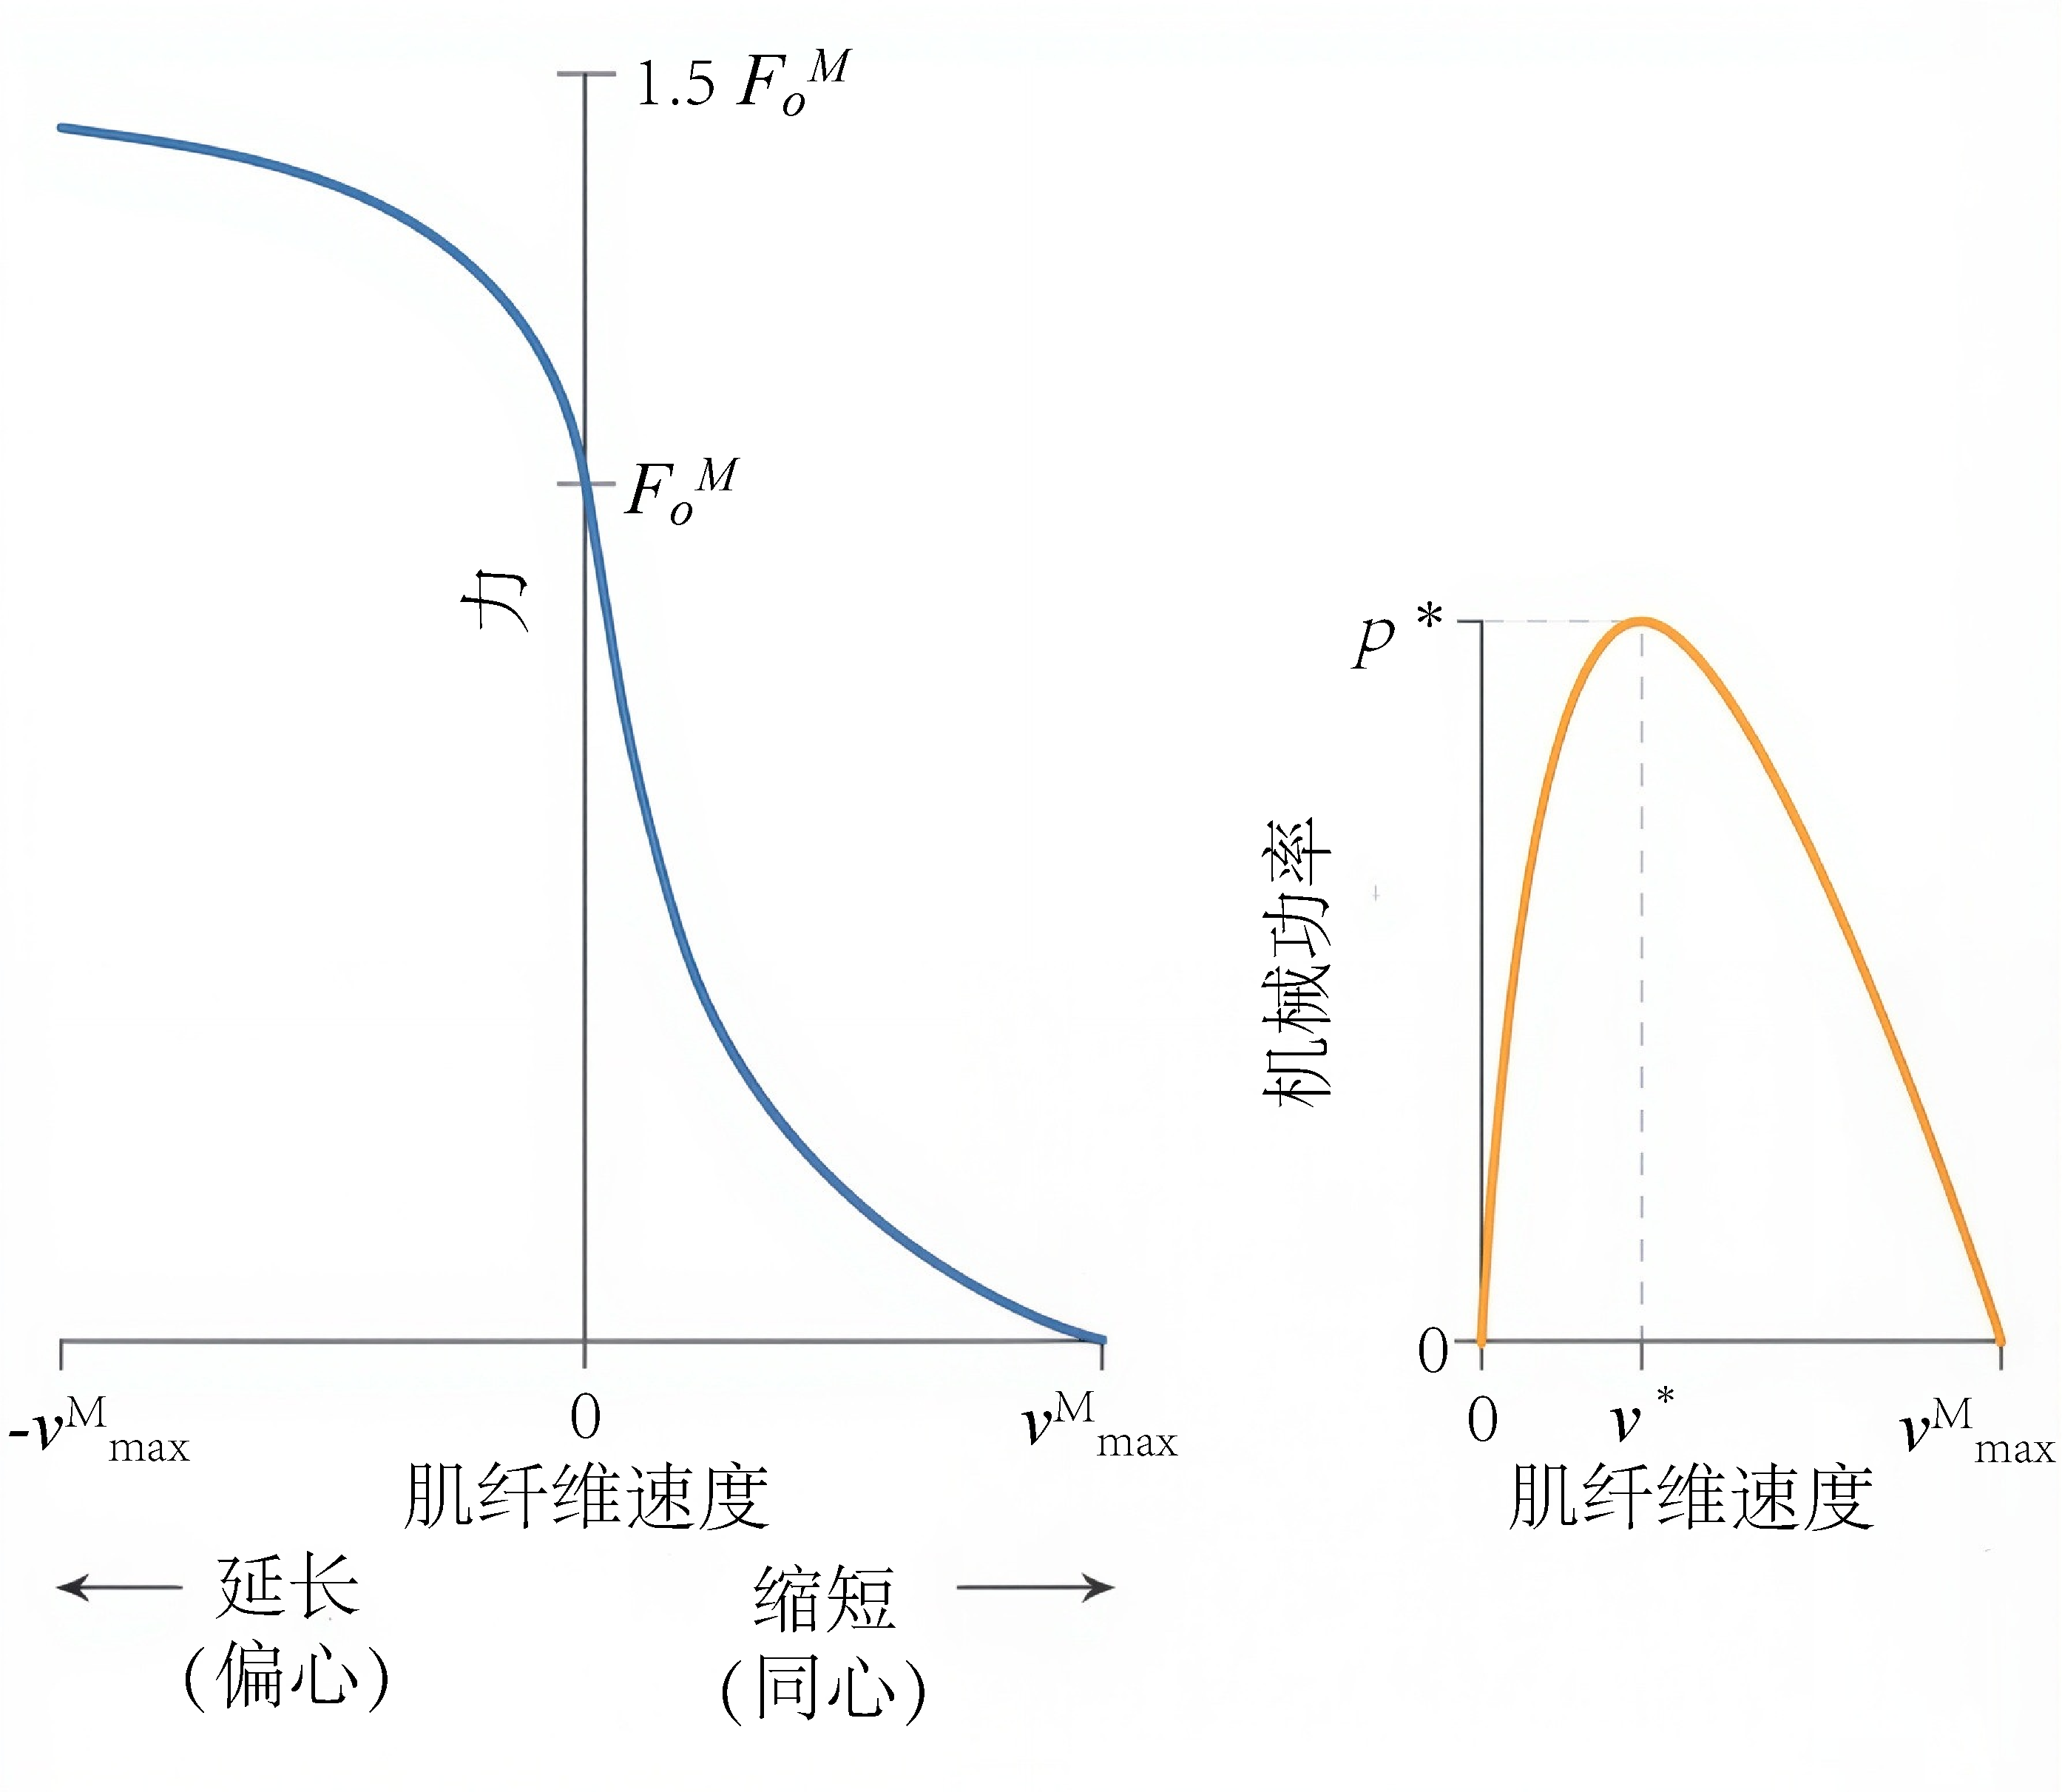
\includegraphics[width=0.7\linewidth]{chap4/4_9}
	\caption{肌纤维\textit{力}和\textit{功率}是\textit{肌纤维速度}的函数。
		肌纤维伸长时,力产生能力增加;
		缩短时,力产生能力降低(左)。
		\textit{机械功率}是力与速度的乘积,在最大缩短速度($v^*$;右)的约三分之一处达到最大值($p^*$)。 \label{fig:4_9}}
\end{figure}

力量取决于速度的原因如下。
肌节通过横桥循环产生力量,在此过程中,肌球蛋白头部与肌动蛋白丝结合并对其施加拉力。
由于此过程需要时间,因此当肌节缩短时,通过横桥循环产生的主动力会减小。
在非常高的缩短速度下,由于粗肌丝和细肌丝相互滑动的速度快于肌球蛋白头部在动力行程中旋转的速度,因此无法产生主动力。
相反,当肌肉拉长时,主动力会增加,因为肌球蛋白的颈部区域在头部与细肌丝分离之前会受到拉力。
非常高的拉长速度会损伤这些结构和其他结构,导致肌肉主动力急剧下降。


肌肉的速度在锻炼时至关重要。
在等长运动中,肌肉在受到相等阻力时被激活。
在这种情况下,肌肉的长度不会改变(即速度为零)。
如果肌肉受到的阻力较小,肌肉就会缩短,这种收缩被称为向心收缩。
相反,如果肌肉受到的阻力较大,肌肉就会伸长,这种收缩被称为离心收缩。


希尔观察到,在向心收缩过程中,随着缩短速度的增加,主动力呈双曲线下降,在最大收缩速度($v_{\text{max}^M}$)时达到零。
在离心收缩过程中,肌肉力量超过其等长收缩过程中的力量,最高可达其最大等长力量的1.5倍左右。


希尔的观察解释了为什么默多克$\cdot$里奇在“推我拉你”实验中费力不讨好,而布伦达$\cdot$比格兰却几乎不费吹灰之力。
该装置迫使里奇的肌肉在图~\ref{fig:4_9}~中“向心”一侧运作,此时它们施加的力量远低于其最大力量。
相比之下,比格兰的肌肉则在力-速度曲线的“离心”一侧运作,此时它们几乎可以施加其最大力量。
里奇向前蹬踏,就像发动机一样,而比格兰向后蹬踏,就像刹车一样。


向心收缩和离心收缩的另一个区别在于肌肉所做功的性质。
向心收缩时,肌肉做正功,因为力和位移的方向相同。
然而,离​​心收缩时,肌肉也做功(即肌肉做功为负),因为力和位移的方向相反。


你可能想知道,在日常生活中,肌肉是否同时做正功和负功。
确实如此!骑车或步行上坡时,你的肌肉主要做正功。
然而,当你走下陡坡时,你的许多肌肉会做负功来控制下坡速度。
有趣的是,做负功会使肌肉酸痛,并促进肌肉再生。


负功理论认为,肌肉理论上可以从外力中获取能量或“充电”。
可惜,这根本不可能发生。
我们的身体无法逆转驱动横桥机制的化学反应,将二磷酸腺苷(ADP)转化回三磷酸腺苷(ATP)。
然而,对于由可充电电池驱动的机器来说,充电是可能的。
例如,传统汽车的摩擦制动器将动能转化为热能,而电动汽车则利用再生制动来捕获和储存这种能量。


力-速度关系对收缩肌肉产生的机械功率有重要影响(图~\ref{fig:4_9},右图)。
当肌肉等长收缩时,可以产生很大的力,但速度为零;
因此,作为力和速度的乘积的机械功率为零。
在缩短速度 及以上时,机械功率也为零,此时速度很大,但不会产生力。
峰值正机械功率出现在大约 $v_{\text{max}^M}$ ,此时力和速度的乘积达到最大值。
功率-速度关系可以很好地预测日常运动的一些特征。
例如,当骑自行车的人感觉到他们的肌肉移动得太快或太慢时,他们就会换挡,远离最大功率范围。


\section{肌肉激活}

我们假设,只要肌球蛋白头部靠近细丝上的结合位点且存在ATP,肌动蛋白和肌球蛋白就能进行横桥循环。
然而,当肌肉放松时,肌动蛋白上的肌球蛋白结合位点会被原肌球蛋白阻断。
当肌肉兴奋时,钙离子被释放到细胞内空间并与蛋白质复合物肌钙蛋白结合,这会导致原肌球蛋白变形,暴露出细丝上的结合位点(图~\ref{fig:4_10})。


\begin{figure}[!htb]
	\centering
	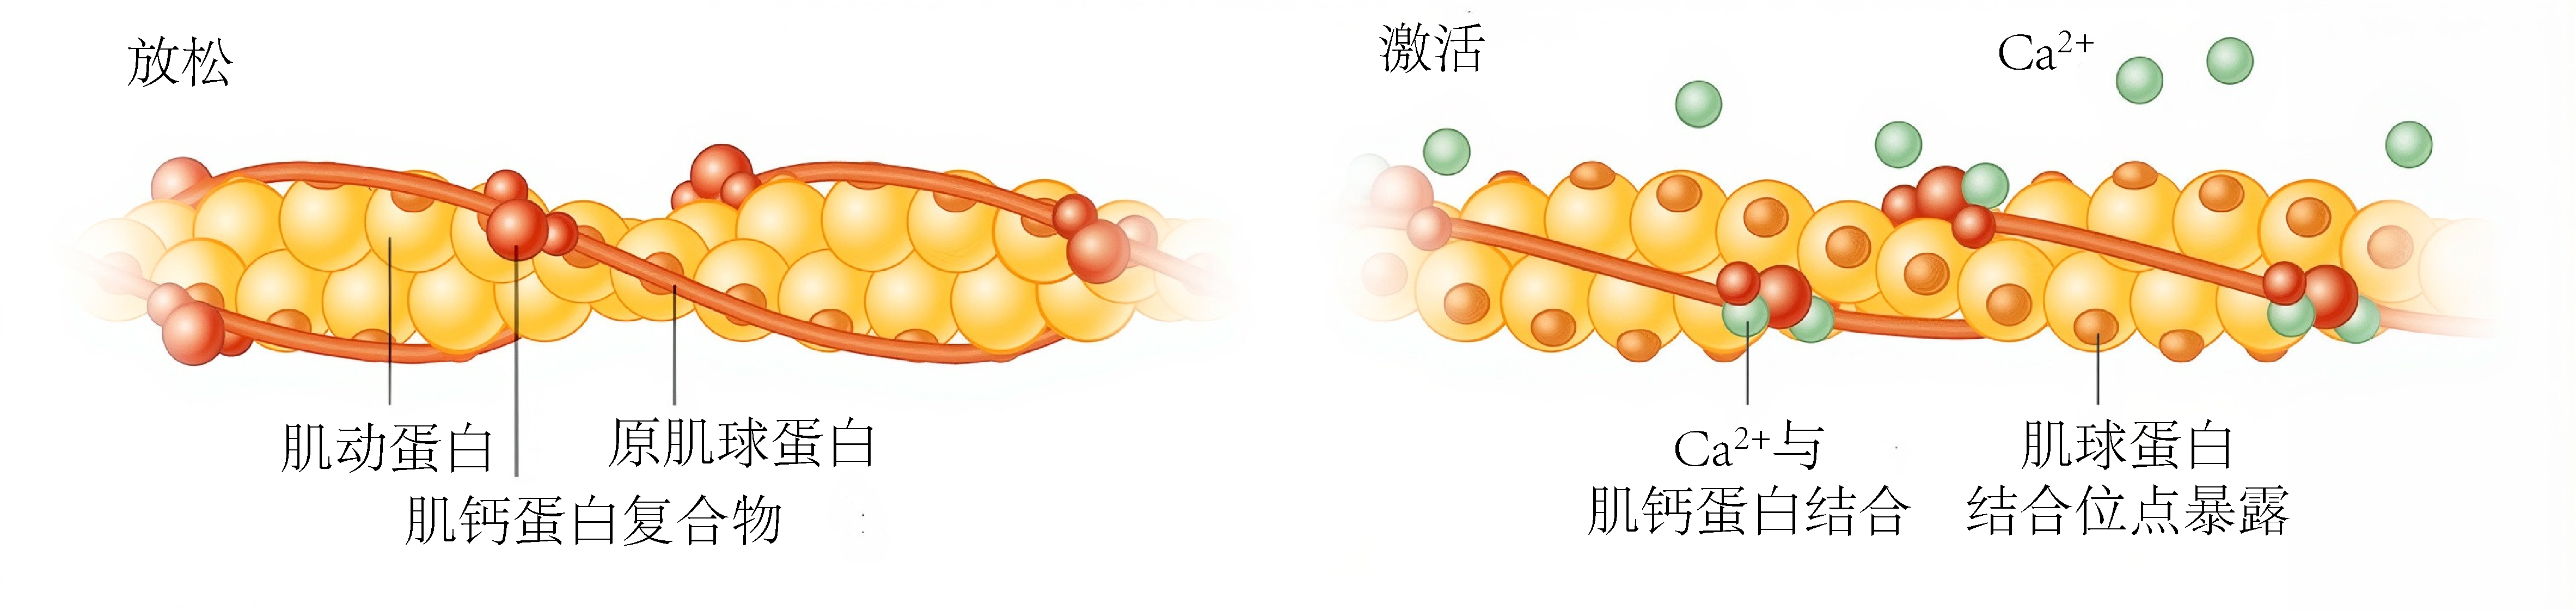
\includegraphics[width=0.85\linewidth]{chap4/4_10}
	\caption{肌肉\textit{激活}过程中的分子变化。
		当肌肉\textit{放松}时(左图),\textit{肌动蛋白}丝上的\textit{肌球蛋白结合位点}被\textit{原肌球蛋白}阻断。
		肌肉激活(右图)会导致肌浆网释放钙离子。
		\ce{Ca^2+}与\textit{肌钙蛋白复合物}结合,导致原肌球蛋白变形,露出肌动蛋白上的肌球蛋白结合位点,从而允许横桥循环开始并产生力量。 \label{fig:4_10}}
\end{figure}

人们不禁会想:钙离子从何而来?
如前所述,它们储存在细胞内一种类似储罐的地方。
它们的释放由中枢神经系统(CNS)控制,它是肌肉发展过程中极其重要的一个环节,我们之前还没有提到过。
肌肉不会自行激活;通常情况下,它们只有在神经系统发出指令时才会活动。


肌纤维具有多种结构特征,使其能够接收来自中枢神经系统(CNS)的信号,并快速传播这些信号,从而沿着整个细胞释放钙离子。
运动神经元通过一个称为神经肌肉接头(neuromuscular joint)的特殊突触与每根肌纤维连接(图~\ref{fig:4_11})。
来自中枢神经系统(CNS)的兴奋信号会导致一种名为乙酰胆碱的神经递质跨神经肌肉接头突触转移。
这种转移触发细胞膜去极化,并导致正钙离子从肌浆网流出。
横轴管系统(通常简称为 T 小管)确保去极化沿着整个肌纤维快速传播。
T 小管是由细胞膜(称为肌膜)在细胞内延伸,将膜状指状结构伸入细胞质时形成的。
终末池位于T小管附近,是肌浆网的延伸,负责储存钙离子。
当细胞去极化时,钙离子会被释放到细胞内,从而启动横桥循环。


\begin{figure}[!htb]
	\centering
	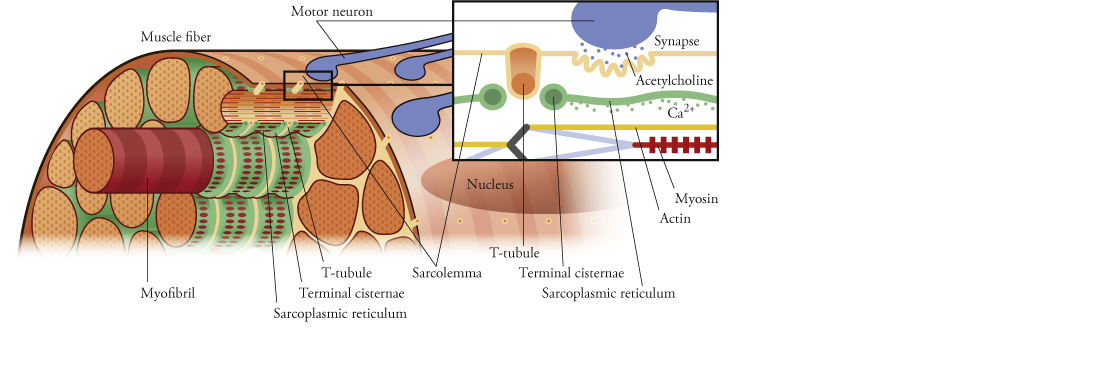
\includegraphics[width=0.95\linewidth]{chap4/4_11}
	\caption{肌纤维的结构使得动作电位能够快速传播,并协调整个长度上的横桥循环。 \label{fig:4_11}}
\end{figure}

当来自中枢神经系统的兴奋信号结束时,细胞开始将钙离子泵回肌浆网。
由于钙离子是逆浓度梯度运输的,因此钙离子的再吸收过程比释放过程慢。


到目前为止,我们仅研究了中枢神经系统如何激活肌肉。
但它的工作远未完成!它还需要告诉肌肉应该用力还是轻柔地拉动。
中枢神经系统利用上述机制,通过两种方式调节肌肉产生的力量:速率编码和运动单元募集。
我们将在接下来的两节中详细阐述这些机制。


\section{速率编码}

信息以电脉冲(称为动作电位)的形式在运动神经元中编码和传输。
通常,激活信号来自大脑,但也可以通过电流通过其支配的运动神经元来人工刺激肌肉。
功能性电刺激疗法利用了这一特性,通过电刺激脊髓损伤导致瘫痪的患者的外周运动神经元。
功能性电刺激系统可用于增强肌肉并产生协调运动,例如划船、抓握和骑自行车,正如我们在第一章中看到的。


对运动神经元施加短促的电刺激,只要刺激电压超过阈值,就会引起其所支配的肌纤维发生“抽搐”(图~\ref{fig:4_12})。
在电脉冲施加和力产生之间,存在一个短暂的延迟,因为去极化会传播并释放钙离子。
随后,纤维力迅速上升,达到峰值,然后相对缓慢地回落至零,因为再摄取过程会将钙离子泵出细胞内空间。


\begin{figure}[!htb]
	\centering
	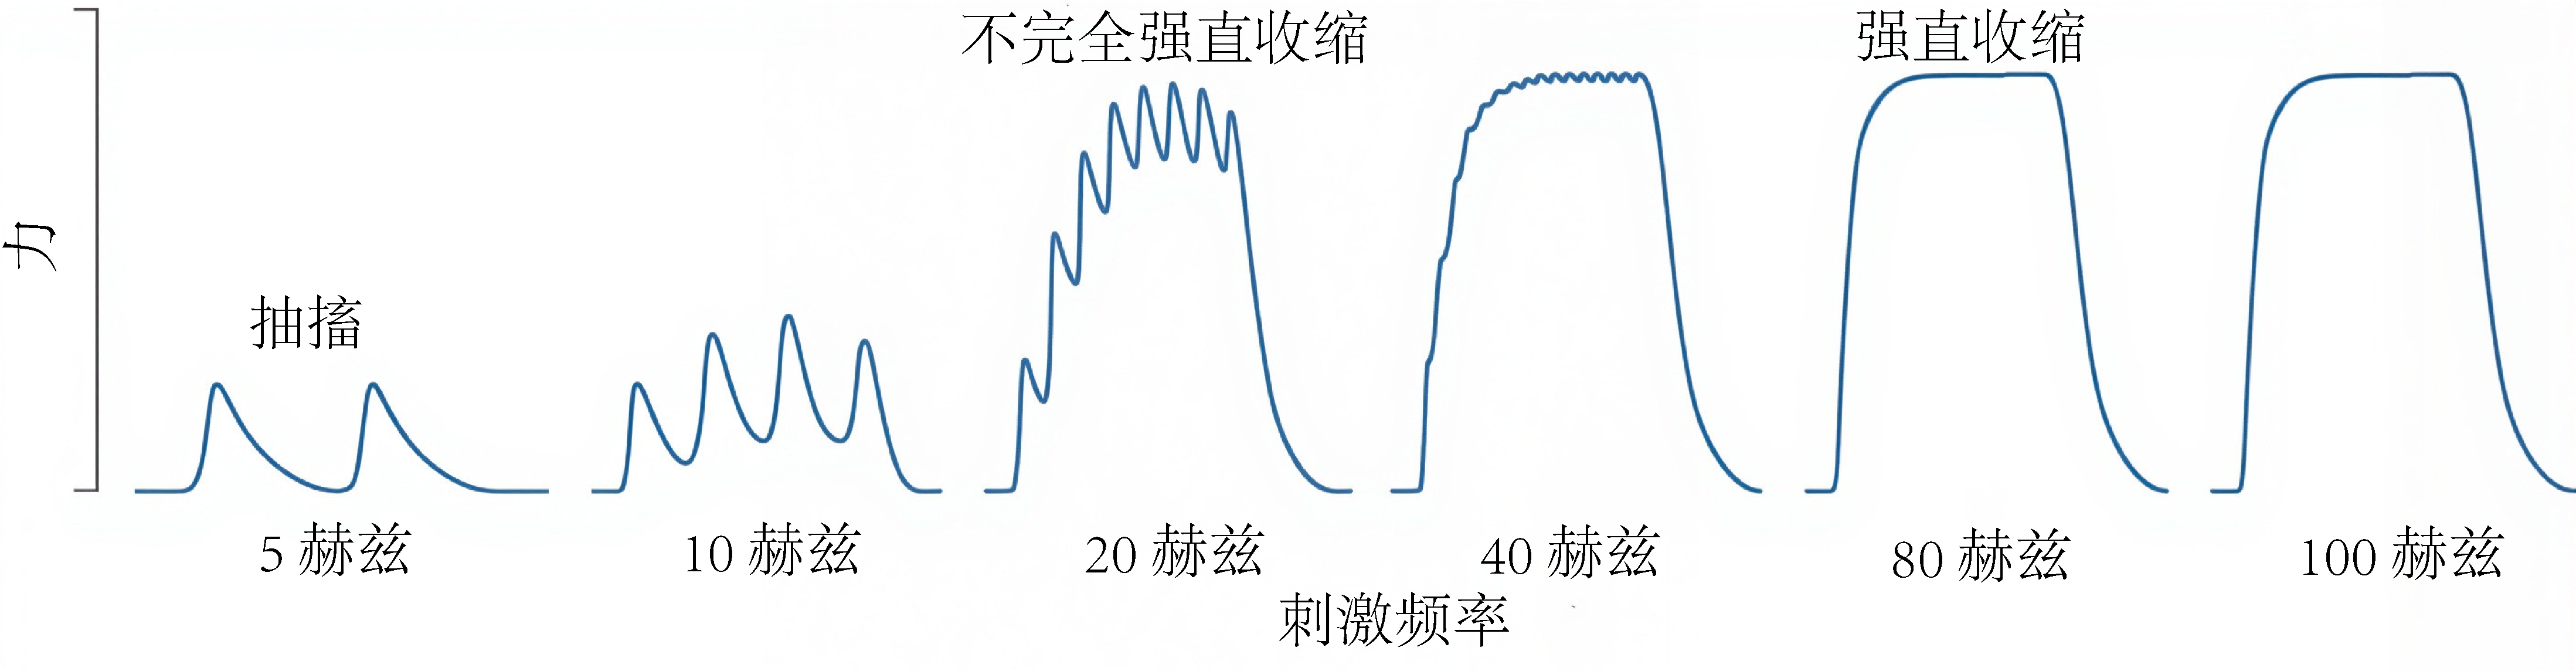
\includegraphics[width=1.0\linewidth]{chap4/4_12}
	\caption{不同\textit{刺激频率}产生的肌肉力量。
		纤维力量受刺激频率(速率编码)调节,产生从\textit{抽搐}(左)到\textit{强直收缩}(右)的各种力量反应。 \label{fig:4_12}}
\end{figure}


刺激肌纤维通常不会使其产生单次抽搐;而是以特定速率施加一系列或一连串脉冲。
如果两次脉冲间隔足够近,第二次抽搐会在第一次脉冲的力完全衰减至零之前开始,从而产生高于第一次的第二个力峰值。
随着脉冲序列频率(或“发放频率”)的增加,峰值力也会增加——直到达到阈值刺激频率,此时纤维力达到稳定水平,峰值力在更高频率下不再增加。
该阈值刺激频率称为强直频率。
在强直频率或以上运作的肌肉被称为融合性强直(离散的抽搐融合在一起形成平滑的力分布);在较低频率下,肌肉被称为未融合性强直。
通过改变刺激频率,肌肉力可以从抽搐到强直进行大约四倍的调节。
换句话说,力的调节可以用刺激的速率来表示,因此称为速率编码。


当然,如果速率编码是调节力量产生的唯一机制,那么许多动作将无法实现。
许多肌肉需要超过四倍的力量变化才能完成其所需的功能范围,如果次最大肌肉力量像图~\ref{fig:4_12}~所示那样波动,我们的动作就会不稳定。


\begin{figure}[!htb]
	\centering
	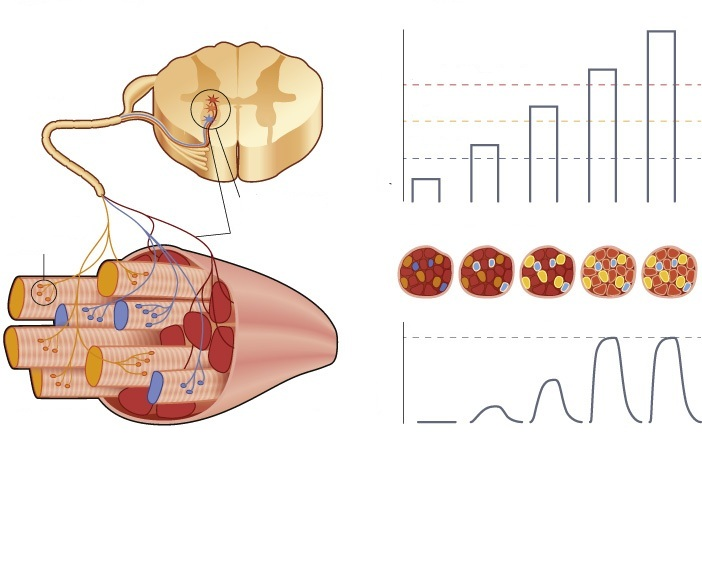
\includegraphics[width=1.0\linewidth]{chap4/4_13}
	\caption{运动单元募集。
		一个运动单元由一个运动神经元及其支配的肌肉纤维组成。
		图中显示了 3 个运动单元(蓝色、橙色和红色)(左图);
		中枢神经系统通过调节被募集的运动单元数量来调节肌肉力量(右图)。 \label{fig:4_13}}
\end{figure}


\section{运动单位募集}

正如预期,控制肌肉力量产生的第二种机制涉及调节控制信号的幅度,而不是频率。
神经系统通过只调动部分肌肉纤维来实现这一点,以完成任何给定的任务:产生较小力量时调动较少的肌肉纤维,产生较大力量时调动较多的肌肉纤维(图~\ref{fig:4_13})。
在次最大努力时,一些肌肉纤维处于非活动状态。


更详细地说,这个过程是这样运作的。
肌肉在功能上被划分为不同的运动单位,这些运动单位由一个运动神经元及其支配的肌纤维组成(图~\ref{fig:4_13},左图)。
运动单位的大小不一,从数十条肌纤维到数千条肌纤维不等。
需要精细控制的小肌肉,例如拇指肌肉,每个运动神经元仅包含少量肌纤维;而控制较粗略的大肌肉,例如背部肌肉,每个运动神经元则包含许多肌纤维。
通常,属于一个运动单位的纤维不会聚集在一起,而是分布在整个肌肉中。
因此,相邻的纤维通常属于不同的运动单位,并且由特定运动神经元支配的纤维可能位于多个肌束中。
中枢神经系统会根据任务需求调整被募集的运动单位数量(图~\ref{fig:4_13},右图)。


运动单元的募集遵循特定的顺序,称为有序募集,正如亨尼曼(Henneman)的尺寸原则\cite{henneman1965functional}所述。
为了产生较小的力量,中枢神经系统(CNS)仅募集小型运动单元。
随着所需肌肉力量的增加,中枢神经系统也会逐渐募集更大的运动单元。
小型和大型运动单元的区别不仅仅在于尺寸:优先募集的小型运动单元也更耐疲劳。
因此,在进行低强度运动时,中枢神经系统会选择性地募集小型纤维,以避免肌肉疲劳。
有序募集的重要性将在第~\ref{chap:chap5}~章中详细讨论。


与有序的运动单元募集不同,外部施加的电刺激并不会根据亨尼曼的大小原则募集运动单元。
当肌肉受到外部刺激时,大型运动单元会与小型运动单元同时被募集\cite{gregory2005recruitment}。
这对功能性电刺激具有重要意义。
尤其是在低水平刺激下募集大型易疲劳的纤维,会使其难以精确调节力量,并导致快速疲劳。


显然,如果我们能够在瘫痪患者中诱导有序募集,治疗质量将得到提升。
我实验室最近的实验表明,可以通过光学控制激活已改变为对光有反应的运动神经元,从而人工实现有序募集\cite{llewellyn2010orderly}。
这项技术最终可能为脊髓损伤和其他运动障碍患者带来更有效的疗法和治疗。



\section{肌电图}

当肌肉受到神经系统的刺激时,会产生一个微小的电信号。
我们刚刚看到,神经系统通过速率编码和运动单元募集来调节肌肉产生的力量。
粗略地说,通过运动神经元到达肌肉的刺激越大(无论是来自更高的频率还是更大的募集量),电信号就越大。
因此,我们可以使用\textit{肌电图}来测量肌肉活动水平,顾名思义,肌电图就是记录肌肉中的电活动。
如果我们将\textit{肌电图}电极连接到放大器和扬声器,我们就能听到肌肉的运动。
由于本书中我们会经常讨论使用\textit{肌电图}信号的研究,因此了解这些测量的基本原理非常重要。


为了记录肌肉活动,我们要么将电极贴到皮肤上进行“表面”肌电图,要么将导线插入肌肉进行肌内肌电图。
表面电极用于记录大块表层肌肉的活动,而肌内电极最适合较小或较深的肌肉。
在大多数设置中,每块肌肉使用一对电极(参考电极和信号电极);
因此,测得的时间序列代表肌肉内所有募集的运动单元的发放组合,并且可能包括周围的肌肉。
进一步复杂化地是,测量的幅度对电极相对于神经和肌肉纤维的位置很敏感(这可能难以精确控制,尤其是在运动过程中)。
因此,原始肌电图信号噪声很大,难以解释。


测量到的肌电信号通常会经过滤波和其他处理,以提高其可解释性(图~\ref{fig:4_14})。
我们通常对肌电信号进行高通滤波以消除随时间变化的漂移,然后对其进行整流和低通滤波,以获得一个包络,该包络可以指示肌肉活动幅度随时间的变化。
最后,我们根据在最大自主收缩或高强度动态运动期间收集的校准测量值对肌电信号进行归一化。
最终结果可以表示肌肉活动量占其最大值的百分比。


\begin{figure}[!htb]
	\centering
	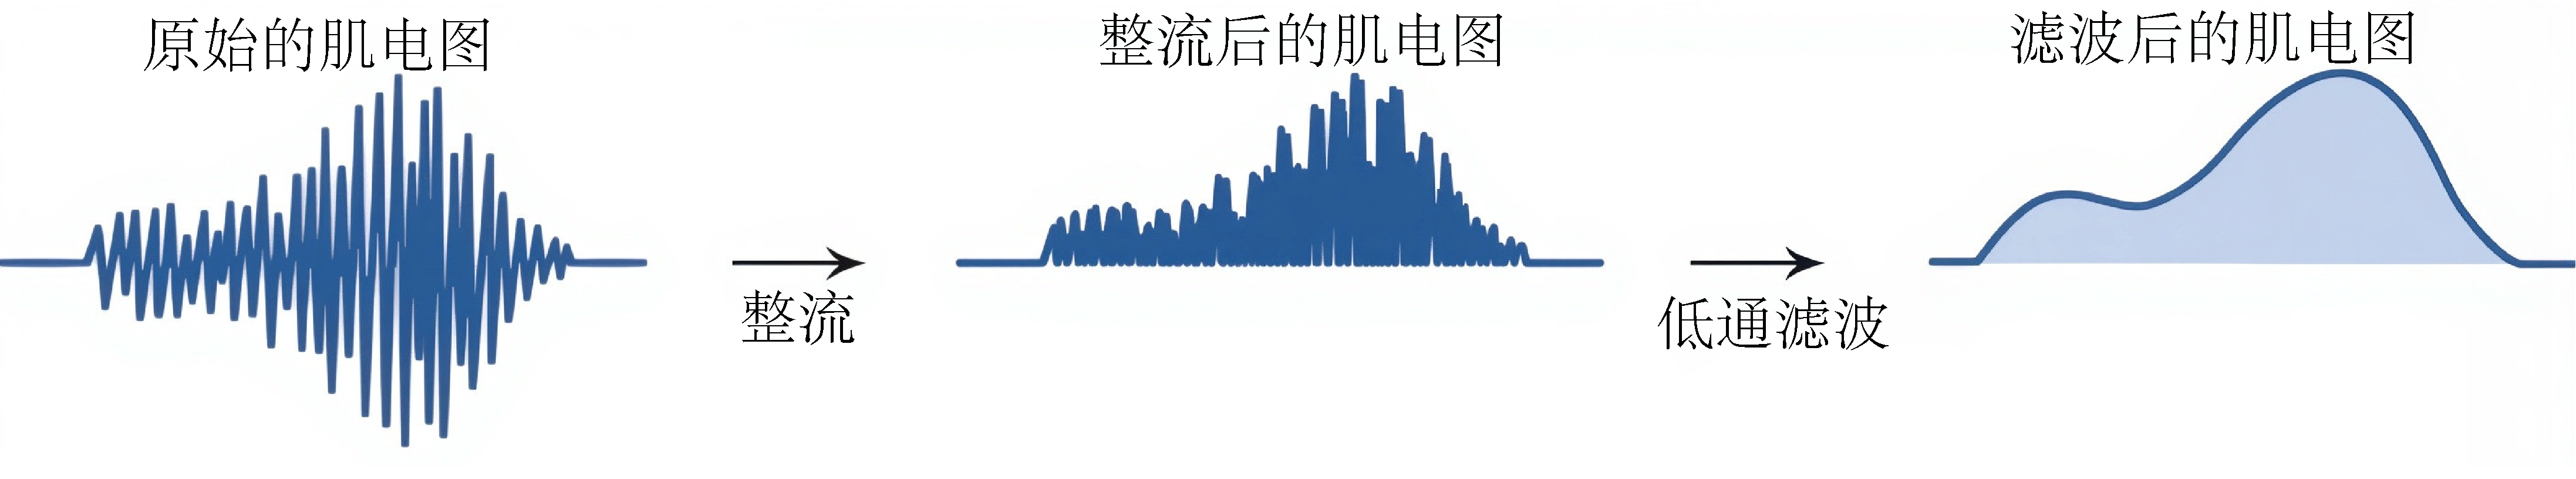
\includegraphics[width=1.0\linewidth]{chap4/4_14}
	\caption{\textit{肌电图}信号的处理。
		原始\textit{肌电图}信号的幅度会随着运动单元发放频率的增加和更多运动单元的募集而增大。
		为了便于解读,原始\textit{肌电图}信号通常经过高通滤波、整流、低通滤波,然后归一化至最大信号。 \label{fig:4_14}}
\end{figure}


在处理\textit{肌电图}信号时,通常会引入 2 种延迟,以将信号与肌肉的力量产生联系起来。
首先,非零\textit{肌电图}信号的出现和非零肌肉力量之间存在延迟;
延迟的持续时间可能因电极位置和肌肉种类而异。
第二个延迟是由于激活动力学造成的,如下所述。
\textit{肌电图}提供肌肉激活的总体测量,包括来自速率编码和肌肉募集的信息。
经过适当校准后,\textit{肌电图}可以成为研究肌肉协调性和测试肌肉激活模拟准确性的有用工具。


\section{肌肉激活动力学建模}

既然我们已经了解了一些肌肉生物学的基础知识,我们可以构建工程模型来描述肌肉力学。
为此,我们需要表征从肌肉兴奋到肌肉激活的转变,即所谓的激活动力学,并建立表示肌肉收缩动力学的方程(图~\ref{fig:4_15})。
下文我们将讨论激活动力学;收缩动力学将在下一章介绍。


\begin{figure}[!htb]
	\centering
	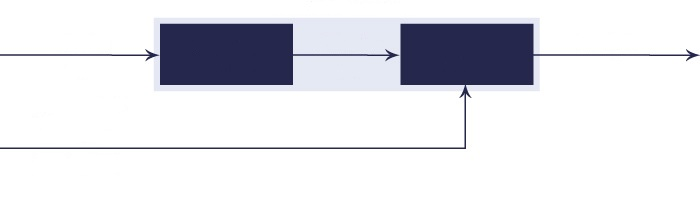
\includegraphics[width=1.0\linewidth]{chap4/4_15}
	\caption{肌肉-肌腱模型的输入和输出。
		在肌肉-肌腱执行器的计算模型中,我们假设激活动力学的过程(将激励 $(u(t))$  转换为激活 $(a(t))$)不同于收缩动力学,后者将肌肉-肌腱长度 $l^{\text{MT}(t)}$ 和速度 $v^{\text{MT}}(t)$ 与肌肉力 $F^{\text{M}}(t)$ 关联起来。 \label{fig:4_15}}
\end{figure}


速率编码和运动单元募集的影响可以纳入激活动力学的数学模型中。
肌肉激活的建模策略有很多;我的实验室采用以下方法。
该模型接受一个时变函数 $u(t)$ 作为输入,该函数描述了从神经到肌肉的兴奋信号强度。
其输出 $a(t)$ 是激活值,表示细胞内钙离子的可用性,从而表示横桥循环发生的程度。
$u(t)$ 和 $a(t)$ 均在 0(无兴奋;无横桥循环)和 1(最大兴奋;融合强直信号,所有运动单元均已募集)之间变化。


我们用经验确定的一阶常微分方程来模拟激发和激活之间的关系:
%
\begin{equation} \label{eq:4_1}
	\begin{aligned}
		\hat{a}(t) = \frac{u(t) - a(t)}{\tau} \\
		\text{其中,} \tau =
	\end{aligned}
\end{equation}


参数 A 和 D 分别表示激活和失活时间常数。
如上所述,A 小于 D;典型值分别为 10 毫秒和 40 毫秒,但这些值可能会随年龄、肌肉成分和其他因素而变化。
图~\ref{fig:4_16}~显示了当输入 $u(t)$ 为方波时,该微分方程的典型解。

\begin{figure}[!htb]
	\centering
	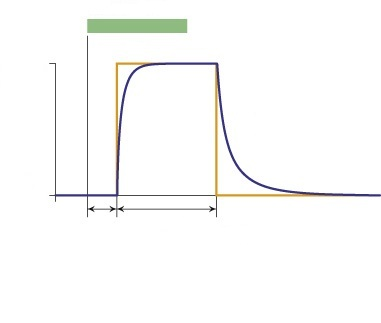
\includegraphics[width=0.6\linewidth]{chap4/4_16}
	\caption{激活动力学计算模型使用一阶常微分方程将激励 $(u(t))$ 与激活 $(a(t))$ 联系起来。
		激励通常滞后于测量的肌电信号,而力的产生则滞后更远。 \label{fig:4_16}}
\end{figure}


\section{力-长度-速度-激活关系建模}

如我们所见,肌肉产生的力量取决于其纤维的长度和速度。
肌肉力量也受运动单元发放率和募集的调节。
如图~\ref{fig:4_17}~所示,力量、长度和速度之间的函数关系可以在最大激活状态(a(t) = 1)下得到说明。
其中,特定长度和速度下的力产生能力仅仅是力-长度曲线和力-速度曲线上相应值的乘积。
请注意,此图的横截面由保持一个变量(长度或速度)恒定而创建,分别以蓝色和绿色显示,与我们已经看到的主动力-长度曲线和力-速度曲线完全相同。
在图~\ref{fig:4_18}~中,我们看到了亚最大激活状态(a(t) < 1)的影响,它使表面图向下缩放。
力-长度关系中的被动成分未在图~\ref{fig:4_17}~或图~\ref{fig:4_18}~中显示,但它始终在健康肌肉中产生力量,并且不依赖于激活状态。

\begin{figure}[!htb]
	\centering
	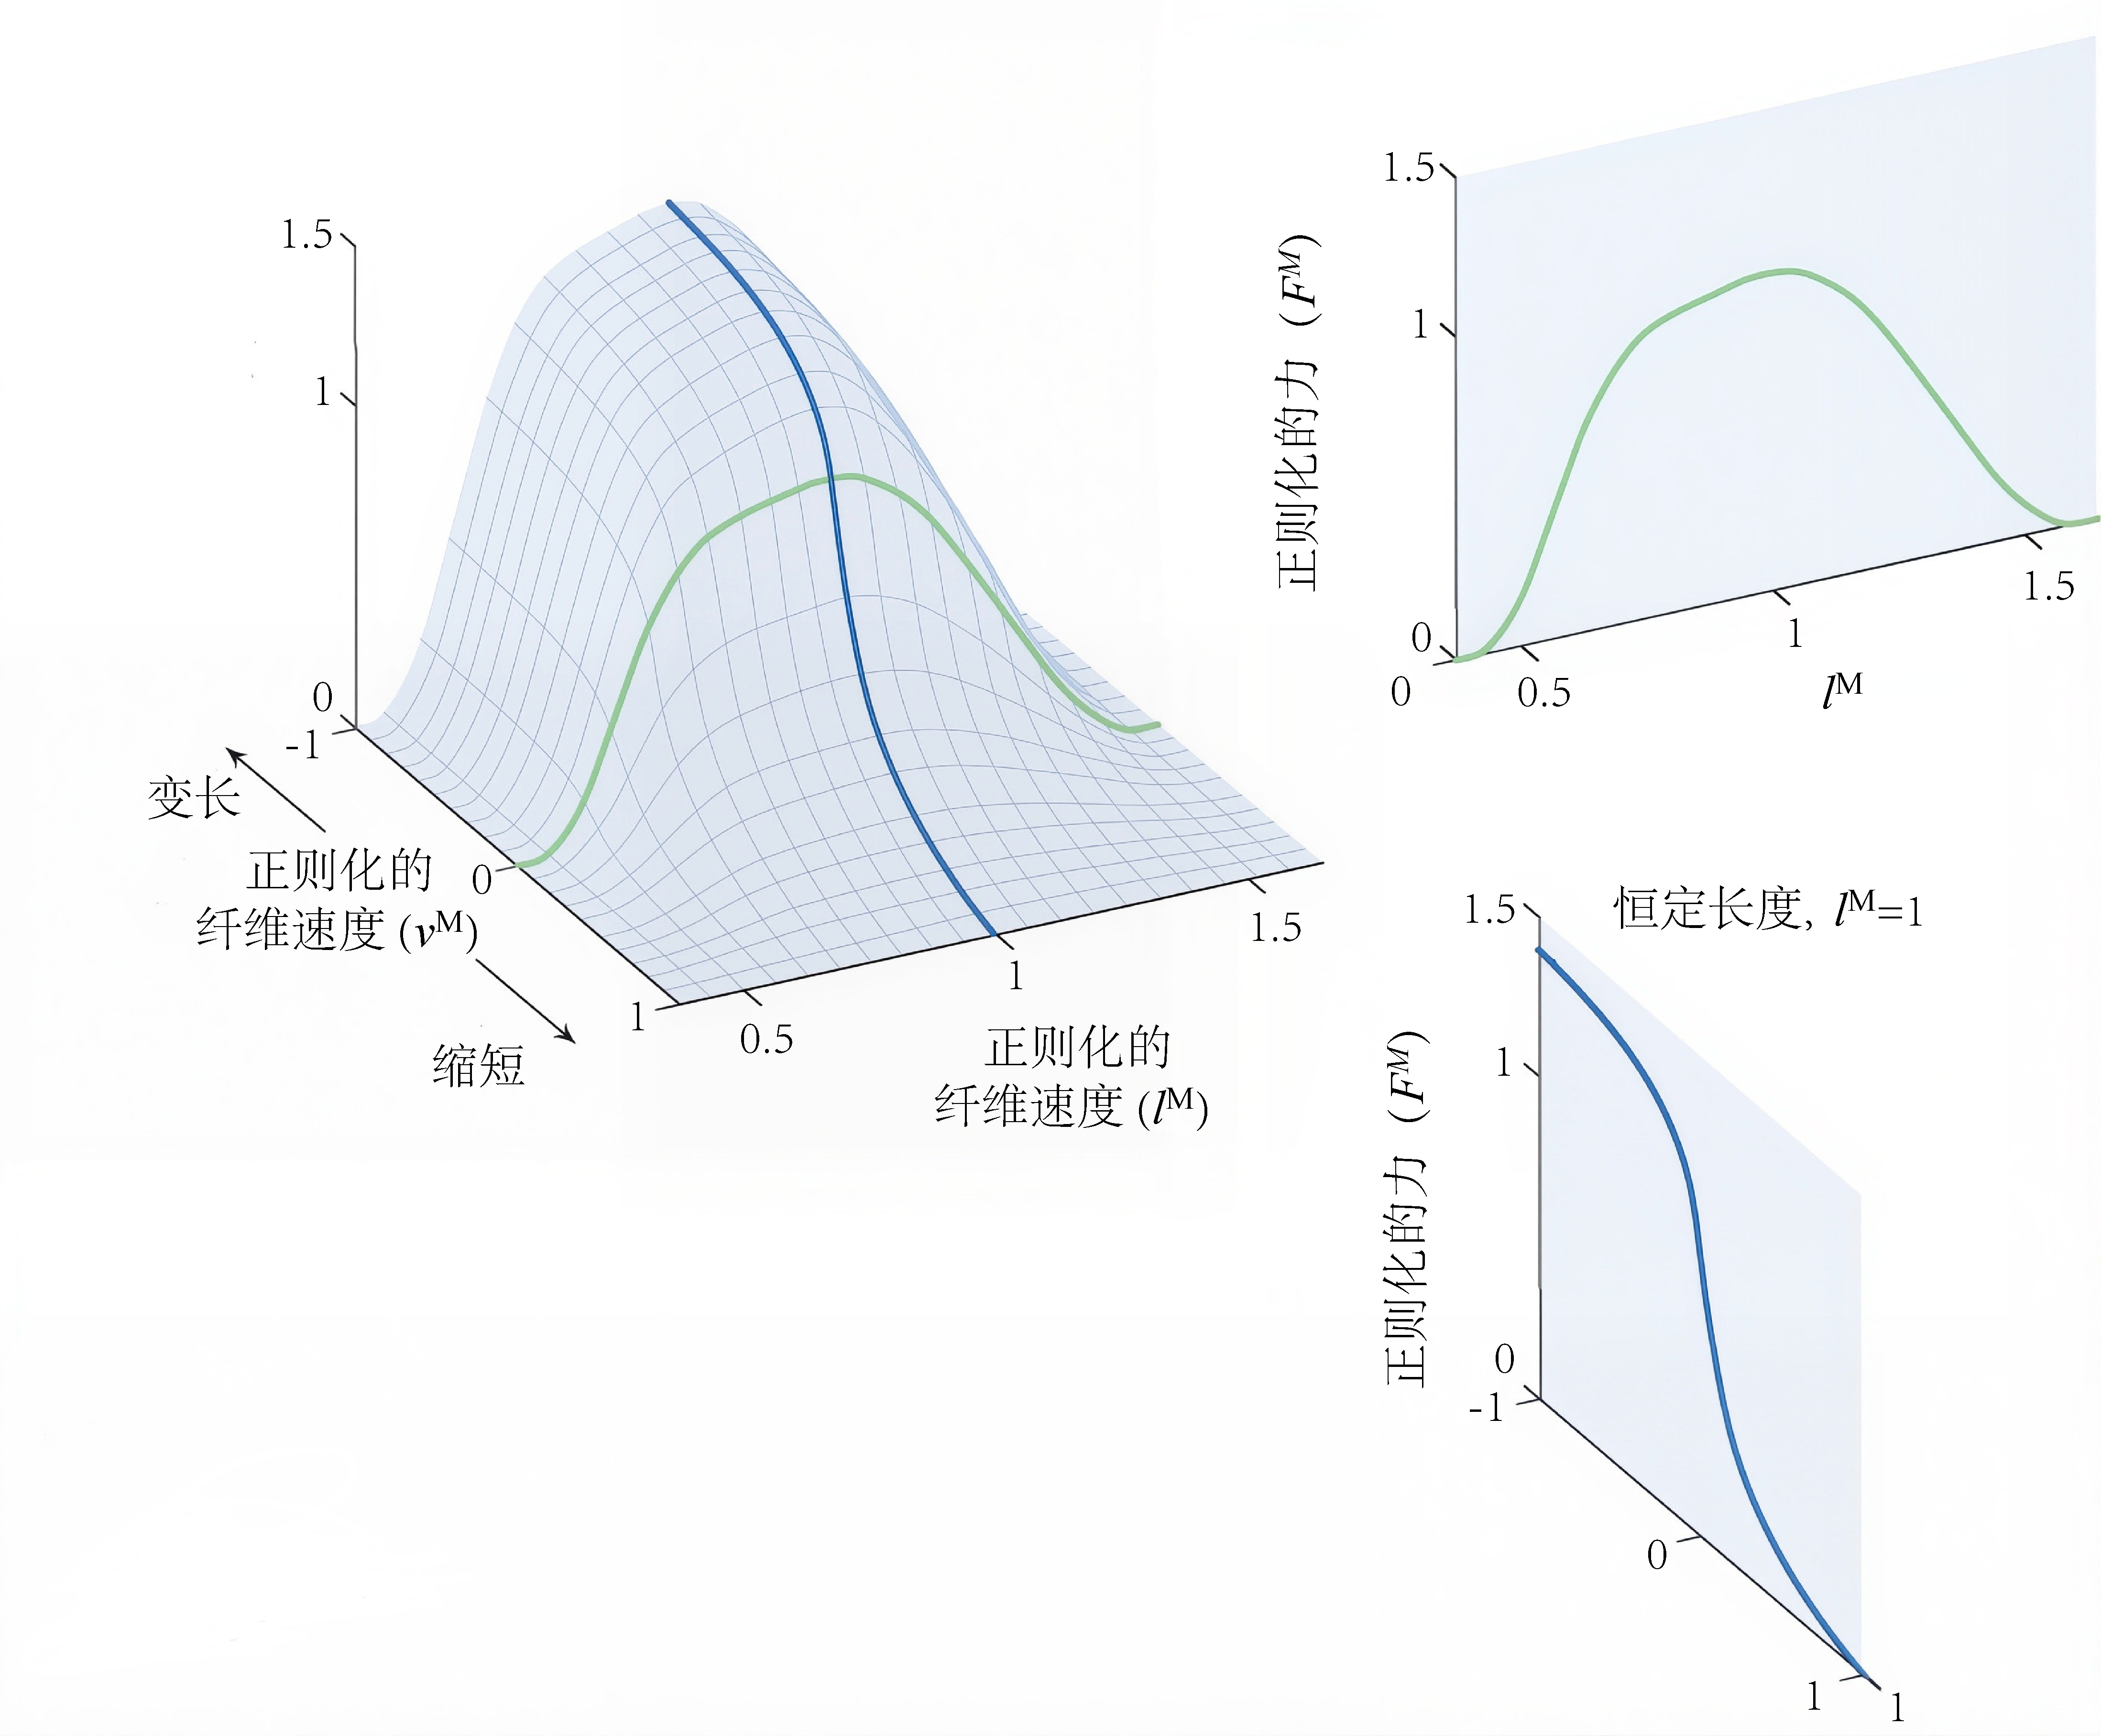
\includegraphics[width=1.0\linewidth]{chap4/4_17}
	\caption{肌肉产生力量的能力随纤维长度和速度而变化\cite{lieber2002skeletal}。 \label{fig:4_17}}
\end{figure}


\begin{figure}[!htb]
	\centering
	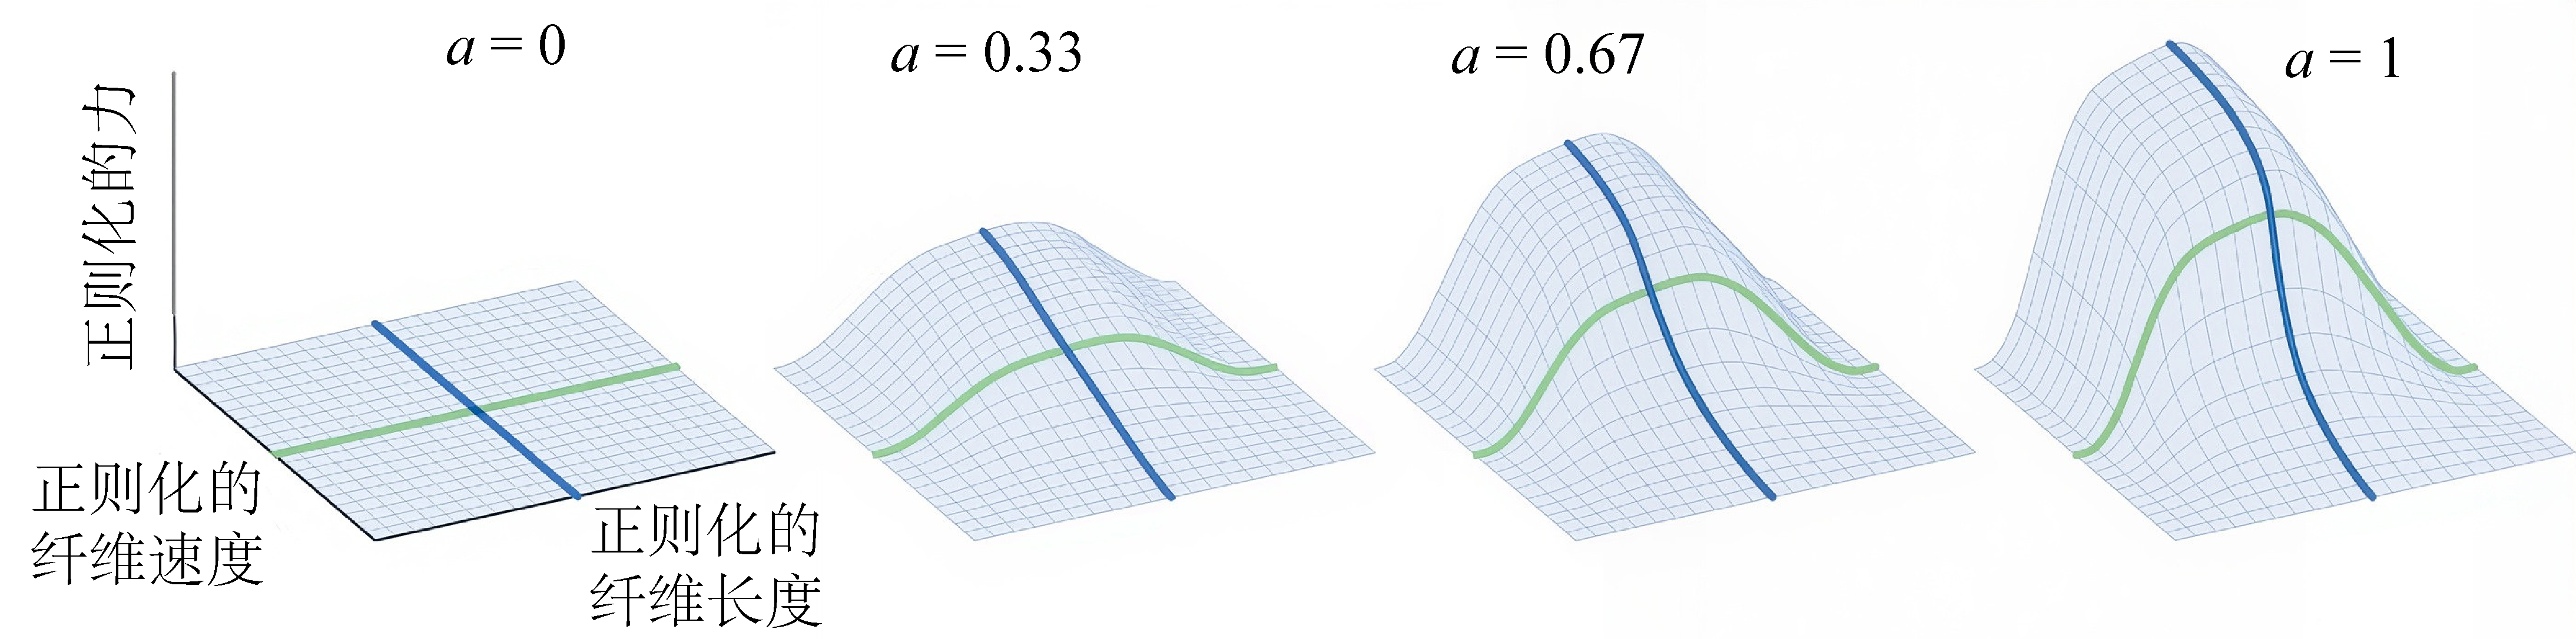
\includegraphics[width=1.0\linewidth]{chap4/4_18}
	\caption{神经系统通过速率编码和运动单位募集来调节肌肉力量,总体上由肌肉激活(a)建模。 \label{fig:4_18}}
\end{figure}


当然,图~\ref{fig:4_18}~所示的模型是对真实肌肉行为的简化。
例如,我们假设纤维长度、纤维速度和激活度会独立地影响肌肉力量的产生。
在真实肌肉中,这些关系更为复杂。
此外,力量的产生还取决于过去的状态以及温度和疲劳程度。
然而,正如我们将看到的,像这样的简化模型是强大的工具,因为它们易于理解,但又足够详细,能够深入了解肌肉驱动的运动。


我们都知道,肌肉的形状和大小千差万别。
下一章将学习如何运用本文介绍的概念,构建肌肉的计算模型——一个可以用来进行数值分析并生成运动模拟的模型。
该模型将使我们能够表征各种条件下不同肌肉的产力特性。







\chapter{肌肉结构和动力学} \label{chap:chap5}


如果你想理解功能,那就研究结构。

\begin{flushright}
	——弗朗西斯$\cdot$克里克
\end{flushright}


\begin{figure}[!htb]
	\centering
	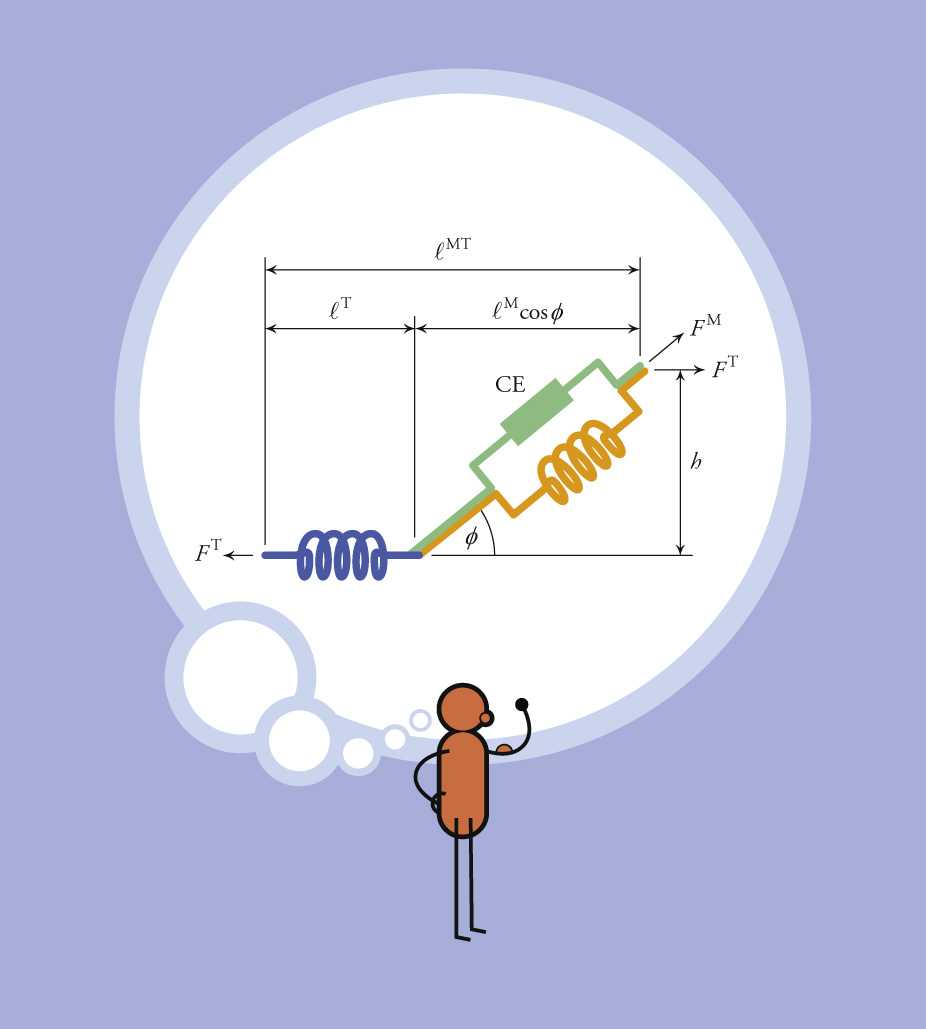
\includegraphics[width=1.0\linewidth]{chap5/5_0}
	% 加星号(*)表示不加编号
	\caption*{ \label{fig:5_0}}
\end{figure}


为了理解人类和动物的运动,研究人员开展了各种各样的实验。
生物力学家通过测量数千人的关节运动、地面反作用力和肌电信号来研究全身运动。
生理学家研究了单个肌肉,以表征肌肉激活和力量产生的动态。
肌肉驱动模拟使我们能够将这 2 个领域联系起来,将全身运动的生物力学测量与针对单个肌肉进行的实验相结合。
我们将在第~\ref{chap:chap10}~至~\ref{chap:chap12}~章中看到,肌肉驱动模拟可以深入了解肌肉在产生运动中的作用,并提供一些在人体运动时几乎无法测量的重要量估计值,例如肌肉产生的力量和它消耗的能量。


肌肉动力学建模对于创建肌肉驱动的运动模拟至关重要。
然而,一刀切的模型并不适用,因为每块肌肉都有其独特的结构来适应其独特的功能。
例如,一些肌肉负责手指的精细运动控制,而另一些肌肉则在运动过程中支撑身体重量(图~\ref{fig:5_1})。
所有骨骼肌都具有肌节的层级排列,但肌肉在几个重要方面存在差异。
这些差异包括它们的大小和结构,以及肌肉纤维的几何排列。
因此,肌肉的计算模型必须捕捉所有肌肉共同的肌肉力量产生特征,同时还要能够表征每块肌肉的独特特征。


\begin{figure}[!htb]
	\centering
	\includegraphics[width=1.0\linewidth]{chap5/5_1}
	\caption{全身肌肉的结构和功能各不相同。
		浅屈指肌(最左侧)通过 4 条肌腱控制手指屈曲;
		宽阔的臀中肌和纤细的股薄肌产生髋关节外展和内收力矩;
		腓肠肌(最右侧)通过较长的跟腱止于跟骨。 \label{fig:5_1}}
\end{figure}


在本章中,我们将了解如何创建一个通用的肌肉力量产生模型,以及如何对其进行定制以代表身体中的几乎任何肌肉。
我们将要描述的肌肉模型属于以 A. V. Hill 命名的一类模型,除了我们在第~\ref{chap:chap4}~章中看到的“推我拉你”实验之外,他还进行了许多肌肉的基础研究。
我的博士生导师 Felix Zajac 改进了 Hill 型模型,并将其带入了现代计算机模拟时代\cite{zajac1989muscle}。
具体来说,Zajac 开发了一个仅包含 4 条通用曲线和 5 个肌肉特定参数的模型,所有这些参数都可以从实验数据中得出并用于调整模型。
Zajac 模型的简单性对于涉及数十块肌肉的动态模拟至关重要,但它足够详细,可以表示不同大小、强度和结构的肌肉的动态。


图~\ref{fig:4_18}~总结了所有肌肉共同的肌肉力量产生特征。
这些特征包括 3 条曲线,描述肌肉长度与其产生的力之间的非线性关系:主动力-长度曲线、被动力-长度曲线和力-速度曲线。
由于肌肉通过肌腱附着在骨骼上,我们还必须考虑这种结缔组织的特性,我们用肌腱的力-长度曲线来描述它。
我们使用 5 个参数缩放这些通用曲线以表示特定的肌肉:
(1)最佳肌纤维长度 $l_o^M$;
(2)最佳纤维长度下的肌纤维羽状角 $\phi_o$ ;
(3)最大等长肌肉力量,$F_o^M$;
(4)最大肌肉收缩速度 $v_\text{max}^M$;
和(5)肌腱松弛长度,$l_s^T$。
本章首先介绍这 5 个特定于肌肉的参数。
我们将了解每个参数如何影响肌肉力量,并将其纳入肌肉-肌腱动力学模型中。


\section{最佳肌纤维长度$l_o^M$}

正如我们在第~\ref{chap:chap4}~章中看到的,肌节能够产生的主动力取决于其长度(图~\ref{fig:4_6})。
肌节能够产生最大等长收缩力的长度称为其最佳长度。
由于肌纤维由多个($n$)个首尾相连的肌节组成,因此肌纤维也存在一个最佳长度($l_o^M$),当其每个组成肌节都达到其最佳长度($l_o^S$)时,肌纤维便会达到该最佳长度:
%
\begin{equation}
	l_o^M = n l_o^S \label{eq:5_1}
\end{equation}

公式~\ref{eq:5_1}~假设肌纤维上串联的所有肌节长度相同。
肌肉在运动过程中会伸长和缩短,这会影响肌节粗肌丝和细肌丝相互滑动时产生的主动力。
最佳长度较长的肌纤维(即串联肌节较多)具有更宽的主动力-长度曲线,并且可以在更宽的长度范围内产生其最大主动力的很大一部分(图~\ref{fig:5_2}顶部)。
增加肌纤维的最佳长度也会增加其最大缩短速度():

\begin{figure}[!htb]
	\centering
	\includegraphics[width=1.0\linewidth]{chap5/5_2}
	\caption{最佳肌纤维长度较长的肌肉,其主动力-长度曲线(上图)更宽,最大缩短速度也更高(下图)。
		请注意,长肌纤维(蓝色)的示意图中,肌节数量是短肌纤维(橙色)的 2 倍,因此长肌纤维在给定时间内可以缩短 2 倍的距离(右下图)。 \label{fig:5_2}}
\end{figure}

\begin{equation}
	v_{\text{max}}^M = n v_{\text{max}}^S \label{eq:5_2}
\end{equation}
%
其中,$v_\text{max}^S$表示肌节的最大缩短速度。
因此,随着肌肉最佳纤维长度的增加,力-速度曲线也会变宽(图~\ref{fig:5_2}底部)。


生物肌肉由长度不同的肌束构成,肌束本身包含长度也不同的纤维,这些纤维甚至可能终止于肌束内。
然而,在我们的模型中,我们假设肌肉中的所有纤维长度相同(许多肌肉,但并非所有肌肉),肌腱动力学模型都做出了这一假设。
我们进一步假设所有纤维都是直的、平行的且共面的。
因此,为了表征肌肉的力-长度和力-速度特性,我们只是放大了肌纤维的相应特性,而这些特性仅仅是肌节相同特性的放大版本。



\section{最佳纤维长度下的肌纤维羽状角$\phi_o$}

肌肉通常通过肌腱附着于骨骼。
在平行纤维肌腱中(例如缝匠肌),其纤维沿着肌腱方向排列(图~\ref{fig:5_3})。
在大多数其他肌肉中,例如股直肌,其纤维与肌腱呈锐角排列;我们称这些肌肉为羽状肌。
“羽状肌”一词源于拉丁语,意为“羽毛状”,而羽状肌的结构确实让人联想到鸟类的羽毛。

\begin{figure}[!htb]
	\centering
	\includegraphics[width=0.8\linewidth]{chap5/5_3}
	\caption{具有不同结构肌肉的例子:
		平行纤维肌肉、单羽状肌肉、双羽状肌肉和多羽状肌肉。 \label{fig:5_3}}
\end{figure}

如果所有肌纤维都附着在肌腱的一侧,我们称该肌肉为单羽状肌;
如果肌纤维附着在肌腱的两侧,则称该肌肉为双羽状肌。
在多羽状肌中,肌腱分支和肌纤维结构可能很复杂。
因此,我们假设给定肌肉中的所有纤维都以相同的角度(称为羽状角 ($\phi$))附着于肌腱,并采用图~\ref{fig:5_4}~所示的肌肉-肌腱几何模型。
由此,我们得到肌纤维中的力 ($F^M$) 和肌腱中的力 ($F^T$) 之间的以下关系:

\begin{figure}[!htb]
	\centering
	\includegraphics[width=0.75\linewidth]{chap5/5_4}
	\caption{肌纤维和肌腱的简化几何表示。
		肌纤维被假设为直的、平行的、共面的、等长的,并以相同的羽状角 ($\phi$) 附着于肌腱。
			当肌纤维缩短或伸长,羽状角增大或减小时,平行四边形的高度 $h$(以及面积)保持不变\cite{zajac1989muscle}。 \label{fig:5_4}}
\end{figure}

\begin{equation}
	F^T = F^M cos(\phi) 
	\label{eq:5_3}
\end{equation}

现在,参考图~\ref{fig:5_4},我们可以解释生物肌肉如何在纤维长度发生变化的情况下保持体积恒定。
随着图中纤维的缩短,想象一下它们以这样的方式缩短,使得图~\ref{fig:5_4}~中的平行四边形保持相同的高度 $h$。
平行四边形的顶部将保持不变,但底部将被向右拉,平行四边形将变得更接近矩形。
然而,只要高度保持不变,面积也将保持不变,这符合平行四边形面积等于其底边和高乘积的几何规则。
我们以二维方式绘制了该图,但三维运动类似,并确保肌肉的体积不变。
简而言之,羽状肌不是通过膨胀来维持体积,而是通过剪切来维持体积。


在上述过程中,羽状角不断增大,从纤维传递到肌腱的力不断减小,直到纤维与肌腱垂直,图中的肌肉呈矩形(即$\phi$ = 90度)。
我们使用参数$\phi_o$表示肌纤维达到最佳长度时的羽状角(即$l^M = l_o^M$)。
我们所描述的固定高度近似法可能会对收缩时明显隆起的肌肉引入误差,但它为研究肌肉结构的功能含义提供了一个简单的几何模型。


除了公式~\ref{eq:5_3}~中表达的关系外,羽状肌在决定肌肉的产力能力方面也起着至关重要的作用。
一般来说,羽状肌角度越大,在给定体积内能够容纳的肌肉纤维越多。
想象一下在矩形房间铺设硬木地板的类似情况:
可以使用相对较少的长木板来延伸房间的长度,或者使用大量较短的木板以对角线方向铺设。
同样,与相同体积的平行纤维肌肉相比,羽状肌的纤维更短,因此主动力-长度曲线和力-速度曲线更窄(图~\ref{fig:5_2})。
当然,羽状肌也包含更多的纤维,其后果将在下一节探讨。



\section{最大等长肌肉力 $F_o^M$}

我们 5 个肌肉参数系列中的第三个参数相对容易理解,但测量起来却不那么容易。
这就是最大等长肌肉力。
它被定义为肌肉在最大程度激活并保持最佳纤维长度时产生的力。


对于活体人体来说,最大等长肌力很难测量,因为我们无法将一块肌肉与其他肌肉分离,并只对该肌肉施加阻力。
因此,我们使用一个称为生理横截面积(PCSA;图~\ref{fig:5_5})的指标。
这是肌肉垂直于纤维方向的横截面积。
需要注意的是,在羽状肌中,该横截面积与肌肉的纵轴倾斜。
最大等长肌力可以通过以下方式估算:

\begin{figure}[!htb]
	\centering
	\includegraphics[width=1.0\linewidth]{chap5/5_5}
	\caption{左图所示的肌肉体积相同,但PCSA(主成分分析面积)、最佳纤维长度和羽状角不同。
		羽状肌越多,产生的主动力越大,但纤维越短;
		因此,其主动力-长度曲线和动力-速度曲线更高,但更窄\cite{lieber2002skeletal}。 \label{fig:5_5}}
\end{figure}

\begin{equation}
	F_o^M = \text{PCSA} \sigma_o^M
	\label{eq:5_4}
\end{equation}
%
其中 $\sigma_o^M$ 是肌肉的比张力(也称为峰值等长应力),即单位面积可产生的最大肌肉力。
在构建健康肌肉模型时,该参数的典型值为 $\sigma_o^M = 0.3 \; \text{MPa}$ 。


在上一节中,我们注意到,羽状肌的纤维比相同体积的平行纤维肌更短,但数量也更多。
因此,尽管羽状肌的力-长度和力-速度曲线较窄,但这些曲线也会更高,因为羽状肌的PCSA(以及因此产生的最大等长力)更大(图~\ref{fig:5_5})。


肌肉纤维的长度和收缩速度不仅仅受其几何形状的影响,我们将在接下来的两节中看到这一点。
尽管如此,我们已经可以观察到肌肉的结构如何影响其所能执行的功能范围:
在其他条件相同的情况下,羽状肌能够比相同体积的平行纤维肌产生更大的力量,但其长度范围较小,收缩速度也较低。



\section{最大肌肉收缩速度$v_\text{max}^M$}

到目前为止,我们已经介绍了 3 个与肌肉纤维几何排列相关的变量。
为了确定肌肉的最大收缩速度,我们现在引入一个概念:
肌肉纤维有 2 种类型:快肌纤维和慢肌纤维。
在单次收缩实验中(图~\ref{fig:4_12}),快肌纤维具有更快的上升时间和松弛时间,并且最大收缩速度也更高——大约为每秒 10 个最佳纤维长度 (10 $l_o^M / s$),而慢肌纤维约为 3 $l_o^M / s$ 个。
哺乳动物的肌肉同时包含这 2 种类型的纤维,但快肌纤维与慢肌纤维的比例会因肌肉的功能而异。
例如,腓肠肌含有大量的快肌纤维,这些纤维在需要快速产生巨大力量的活动(例如短跑)中被募集。
邻近的比目鱼肌主要由慢肌纤维组成,这些慢肌纤维非常适合在长时间站立时产生力量,因为慢肌纤维耐疲劳。


肌纤维不仅以其收缩速度区分,还以其产生ATP的方式区分。
有氧(即利用氧气)产生ATP的肌纤维比无氧(即无氧)产生ATP的肌纤维更耐疲劳。
慢肌纤维往往耐疲劳,而快肌纤维则易疲劳。
人类和其他一些动物拥有第三种肌纤维类型,因此我们通常将肌纤维分为I型(慢速,耐疲劳)、IIA型(快速,中度易疲劳)或IIB型(极快,高度易疲劳)。
通过强化训练可以增加快速且仅中度易疲劳的肌纤维比例。


回想一下第~\ref{chap:chap4}~章,运动单位大小各异,中枢神经系统会按照亨尼曼大小原则(图~\ref{fig:4_13})从小到大依次募集运动单位。
除了大小不同之外,运动单位所含纤维的类型也有所不同,同一运动单位中的所有纤维都属于同一类型。
最小的运动单位通常由 I 型纤维组成,最先被募集,其次是由 IIA 型纤维组成的稍大的运动单位。
最大的运动单位包含 IIB 型纤维,通常最后被募集。
因此,在低激活度下(例如在安静站立时可能观察到),主要募集的是慢肌、抗疲劳的运动单位。
因此,在低激活度下,肌肉的最大收缩速度可能会降低;
然而,在肌肉-肌腱动力学模型中,通常假设其为常数 10 $l_o^M/s$。


粗略地说,家禽和鱼类的可疲劳肌纤维和抗疲劳肌纤维是分开的(图~\ref{fig:5_6})。
相反,哺乳动物的肌肉中可疲劳肌纤维和抗疲劳肌纤维是交替分布的。
这就是为什么鸡肉菜肴可以用白肉或黑肉来制作,而牛肉菜肴却不能。
颜色差异的原因是深色肌肉(或肉)富含一种叫做肌红蛋白的蛋白质,这种蛋白质在肌肉中储存氧气,使肌肉颜色变深,使其更耐疲劳。
鸡腿的深色肉由用于长时间站立和奔跑的腿部肌肉(抗疲劳、慢肌纤维)组成。
白色的胸肉由仅用于短时间飞行的肌肉(可疲劳、快肌纤维)组成。
在人类中,单个肌纤维要么是“深色”的,要么是“白色”,但这两种纤维类型都散布在每块肌肉中。


\begin{figure}[!htb]
	\centering
	\includegraphics[width=0.8\linewidth]{chap5/5_6}
	\caption{鸡肉和鱼类的某些肌肉主要由抗疲劳的慢肌纤维(深色肉)组成,而另一些肌肉则由易疲劳的快肌纤维(白肉)组成。
		在人类和其他哺乳动物中,各种类型的纤维散布在每块肌肉中。
		人体纤维染色图像显示了不同的纤维类型,由 Richard Lieber 提供。 \label{fig:5_6}}
\end{figure}


\section{肌腱松弛长度 $l_s^T$}

到目前为止,我们讨论的所有参数都与肌腱无关。
在我们的希尔模型中,我们将肌腱描述为非线性弹簧。
本节介绍 5 个参数中的第五个参数,称为肌腱松弛长度,以及 4 个通用无量纲曲线中的第四个参数,称为肌腱力-长度曲线。
我们根据应力和应变之间的实验测量结果推导出力-长度曲线(图~\ref{fig:5_7})。


\begin{figure}[!htb]
	\centering
	\includegraphics[width=0.8\linewidth]{chap5/5_7}
	\caption{在该图中,横轴表示肌腱的应变,用其长度相对于静止且未受力时的长度的百分比表示。
		静止长度即为松弛长度,用 $l_s^T$ 表示。
		任意给定时刻肌腱的应变 ($\epsilon^T$) 定义如下: \label{fig:5_7}}
\end{figure}

\begin{equation}
	\epsilon^T = \frac{l^T - l_s^T}{l_s^T} 
	\label{eq:5_5}
\end{equation}
% 
其中 $l^T$ 是肌腱的当前长度,$l_s^T$是其松弛长度。


图~\ref{fig:5_7}~中的纵轴表示肌腱单位横截面积产生的力,称为应力。
在线性弹簧中,应力与应变的关系图是一条直线,其斜率表示弹簧的刚度。
由于肌腱充当非线性弹簧,因此应力-应变曲线不是直线,并且它具有 3 个具有不同刚度特征的区域。
在脚趾区域,当肌腱拉伸约 0\% 到 3\% 时,它会更加柔顺(“有弹性”),随着肌腱的伸长和其组成胶原纤维的展开,其刚度逐渐增加。
在应力-应变曲线的线性区域,当肌腱拉伸约 3\% 到 7\% 时,肌腱具有恒定的刚度;
在此区域,它的行为类似于线性弹簧。
最后,超过 10\% 的应变,肌腱开始出现机械故障,并且存在很高的受伤风险。
我们通常假设内部肌腱(腱膜)和外部肌腱具有相同的材料特性和应变。
有实验证据支持上面给出的应变值,但有人认为肌腱在断裂前可以承受高达 15\% 的更高应变值。


肌腱会影响其所附着肌肉的长度,从而影响其产力能力(图~\ref{fig:5_8})。
如果肌腱的松弛长度相对于肌纤维的长度较短,则肌腱的拉伸几乎不会产生影响:
即使这样的肌腱承受很大的应变,其绝对长度变化(以及肌纤维缩短的量)也只是肌纤维最佳长度的一小部分。
相反,如果肌腱的松弛长度相对于肌纤维的最佳长度较长,则肌肉产力时肌腱会大幅拉伸,导致肌纤维明显缩短,并改变产生的主动力。
图~\ref{fig:5_9}~显示,较长的肌腱还可以增加肌肉-肌腱单元产力的长度范围。
通过这 2 种方式,肌腱都会显著影响肌肉功能。
当然,当肌腱损伤导致肌肉几乎无法使用时,肌腱的作用尤为明显。
正如我们将在第~\ref{chap:chap12}~章中看到的,肌腱在跑步过程中伸展和回缩时也在能量的储存和释放中发挥着重要作用。


\begin{figure}[!htb]
	\centering
	\includegraphics[width=1.0\linewidth]{chap5/5_8}
	\caption{肌腱的柔顺性会影响肌肉力量的产生。
		在图示的两种情况下,平行纤维肌肉在非活动状态时处于最佳长度(上)。
		如果肌腱相对较短且僵硬(左),则肌肉活动时肌纤维的长度变化可以忽略不计。
		如果肌腱较长且柔顺性良好(右),则肌肉活动时肌腱会拉伸,从而缩短肌纤维并减少产生的力量。 \label{fig:5_8}}
\end{figure}


\begin{figure}[!htb]
	\centering
	\includegraphics[width=0.6\linewidth]{chap5/5_9}
	\caption{肌腱柔顺性对主动力-长度曲线的影响。
		增加肌腱相对于最佳肌纤维长度的松弛长度(即增加肌腱柔顺性),可以扩大肌肉-肌腱执行器产生主动力的长度范围。 \label{fig:5_9}}
\end{figure}



\section{测量肌肉特定参数}

总而言之,我们定义了 5 个肌肉特异性参数,列于表~\ref{tab:5_1},这些参数捕捉了身体肌肉之间的大部分变异性。
我们在表 5.2 中列出了下肢主要肌肉的这些参数值。
为方便起见,我们通常将力、速度、肌肉长度和肌腱长度分别除以 、 、 和 来进行归一化,并使用波浪号表示归一化后的量(例如 )。


\begin{table}[htbp]
	\caption{Hill 型模型使用的 5 个肌肉特定参数} \label{tab:5_1} \centering
	\begin{tabular}{ccc} % l水平左居中,c水平居中
		\toprule
		肌肉特异性参数 & 符号 & 典型单位  \\
		\midrule
		最佳纤维长度下的羽状角 & $\phi_o$ &  度 \\
		\midrule
		最大等长力量 & $F_o^M$ &  牛顿 \\
		\midrule
		最大收缩速度 & $v_\text{max}^M$ &  $l_o^M / s$ \\
		\midrule
		肌腱松弛长度 & $l_s^T$ &  厘米 \\
		\bottomrule
	\end{tabular}
\end{table}


\begin{table}[htbp]
	\caption{下肢主要肌肉的肌肉特异性参数值*} \label{tab:5_2} \centering
	\begin{tabular}{ccccc} % l水平左居中,c水平居中
		\toprule
		肌肉 & 最大等长力(牛) & 最佳纤维长度(厘米)& 肌腱松弛长度(厘米) &  羽状角(度) \\
		\midrule
		短收肌 & 626 &  10.3 & 3.5 & 7 \\
		\midrule
		长收肌 & 917 &  10.8 & 13.2 & 8 \\
		\midrule
		大收肌 &  &   &  &  \\
		\midrule
		末梢 & 597 &  17.7 & 8.7 & 11 \\
		\midrule
		坐骨 & 597 &  15.6 & 21.6 & 10 \\
		\midrule
		腰部 & 597 &  13.8 & 4.7 & 12 \\
		\midrule
		近端 & 597 &  10.6 & 4.0 & 18 \\
		\midrule
		股二头肌长头 & 1313 &  9.8 & 32.5 & 10 \\
		\midrule
		股二头肌短头 & 557 &  11.0 & 10.6 & 15 \\
		\midrule
		伸趾长肌 & 603 &  6.9 & 36.9 & 13 \\
		\midrule
		拇长伸肌 & 286 &  7.5 & 32.7 & 11 \\
		\midrule
		屈趾长肌 & 423 &  4.5 & 37.9 & 13 \\
		\midrule
		拇长屈肌 & 908 &  5.3 & 35.4 & 15 \\
		\midrule
		腓肠肌外侧头 & 1575 &  5.9 & 37.6 & 12 \\
		\midrule
		腓肠肌内侧头 & 3116 &  5.1 & 39.9 & 10 \\
		\midrule
		臀大肌 &  &   &  &  \\
		\midrule
		上 & 984 &  14.7 & 4.9 & 20 \\
		\midrule
		中 & 1406 &  15.7 & 6.8 & 21 \\
		\midrule
		下 & 948 &  16.7 & 7.0 & 22 \\
		\midrule
		臀中肌 &  &   &  &  \\
		\midrule
		前 & 1093 &  7.3 & 5.6 & 18 \\
		\midrule
		中 & 765 &  7.3 & 6.5 & 18 \\
		\midrule
		后 & 871 &  7.3 & 4.5 & 18 \\
		%
		\midrule
		臀小肌 &  &   &  &  \\
		\midrule
		前 & 374 &  6.8 & 1.6 & 10 \\
		\midrule
		中 & 395 &  5.6 & 2.6 & 0 \\
		\midrule
		后 & 447 &  3.8 & 5.1 & 1 \\
		\midrule
		股薄肌 & 281 &  22.8 & 17.2 & 10 \\
		\midrule
		髂肌 & 1021 &  10.7 & 9.6 & 16 \\
		\midrule
		腓骨短肌 & 521 &  4.5 & 14.8 & 12 \\
		\midrule
		腓骨长肌 & 1115 &  5.1 & 33.2 & 14 \\
		\midrule
		梨状肌 & 1030 &  2.6 & 11.5 & 10 \\
		\midrule
		腰大肌 & 1427 &  11.7 & 10.0 & 12 \\
		\midrule
		股直肌 & 2192 &  7.6 & 44.9 & 12 \\
		\midrule
		缝匠肌 & 249 &  40.3 & 12.4 & 2 \\
		\midrule
		半膜肌 & 2201 &  6.9 & 34.8 & 15 \\
		\midrule
		半腱肌 & 591 &  19.3 & 24.7 & 14 \\
		\midrule
		比目鱼肌 & 6195 &  4.4 & 27.7 & 22 \\
		\midrule
		阔筋膜张肌 & 411 &  9.5 & 45.0 & 3 \\
		\midrule
		胫骨前肌 & 1227 &  6.8 & 24.1 & 11 \\
		\midrule
		胫骨后肌 & 1730 &  3.8 & 28.1 & 13 \\
		\midrule
		中间股 & 1697 &  9.9 & 20.2 & 4 \\
		\midrule
		股外侧肌 & 5149 &  9.9 & 22.1 & 15 \\
		\midrule
		股内侧肌 & 2748 &  9.7 & 20.0 & 24 \\
		\bottomrule
	\end{tabular}
\end{table}


目前已开发出多种技术来测量或计算肌肉和肌腱参数的值。
结构参数历来是通过对人类尸体进行测量获得的,而诸如力-速度关系的形状等动态特性通常来自动物肌肉实验。
获取和解释尸体测量值时必须小心谨慎,因为组织特性在死后可能会发生变化;
例如,肌肉脱水会改变肌肉的质量、体积、形状和长度。
此外,尸体测量数据通常取自老年捐赠者的遗体,他们的肌肉可能已经萎缩,因此无法代表经常参与研究的年轻健康受试者。
只要有可能,通常最好使用从被研究对象获得的测量值来校准肌肉骨骼模型,尤其是对于已知个体间差异很大的参数(例如最大等长力)。


肌纤维长度和羽状角可以通过解剖尸体标本或体内超声测量(图~\ref{fig:5_10},左)。
但请注意,最佳肌纤维长度无法通过超声图像确定,因为虽然可以测量肌纤维长度,但尚不清楚该长度与产生最大主动力的长度之间的关系。
肌节长度的测量提供了将测量的肌纤维长度与最佳肌纤维长度关联所需的信息,因为肌节的力-长度曲线是已知的。如果测量肌纤维长度 ($l^M$) 和肌节长度 ($l^S$),则最佳肌纤维长度 ($l_o^M$) 可按如下方式计算:


\begin{figure}[!htb]
	\centering
	\includegraphics[width=0.75\linewidth]{chap5/5_10}
	\caption{成像技术提供了校准肌肉-肌腱动力学模型所需的数据。
		左图为胫骨前肌纤维的超声图像,可测量纤维长度。
		右图为使用双光子显微内窥镜获得的同一块肌肉的肌节图像,可测量肌节长度。
		图片由 Glen Lichtwark 和 Gabriel Sanchez 提供。 \label{fig:5_10}}
\end{figure}

\begin{equation}
	l_o^M = l^M \times \frac{l_o^S}{l^S}
	\label{eq:5_6}
\end{equation}
%
其中,表示肌节的最佳长度,人体肌肉中估计为 2.7 微米。
有几种技术可以测量整块肌肉的肌节长度。
其中一种方法是激光衍射法,该技术由 Richard Lieber 首创,通过手术暴露肌肉,然后用激光照射肌肉以产生衍射图案\cite{lieber1984sarcomere}。
我的实验室开发了一种侵入性较小的方法\cite{llewellyn2008minimally},使用针头大小的微型内窥镜对体内肌节长度进行成像(图~\ref{fig:5_10},右)。


由于腱膜位于肌肉内部,难以测量,因此在尸体标本或成像实验中难以确定肌腱松弛长度。
在肌肉-肌腱动力学模型中,确定肌腱松弛长度的一种策略是:测量尸体标本的肌纤维长度、肌节长度和关节位置,然后在模型中设定肌腱松弛长度,使肌纤维长度和肌节长度与同一姿势下的尸体测量值相匹配。


如前所述,我们可以通过测量PCSA和特定张力(公式~\ref{eq:5_4})来估算最大等长肌肉力量。
PCSA可以通过测量尸体标本的肌肉质量或使用MRI测量肌肉体积来估算,后者更可取,因为老年供体受试者的肌肉可能出现萎缩。
我们可以根据肌肉体积和最佳纤维长度计算PCSA,如下所示:
\begin{equation}
	\text{PCSA} = \frac{\text{muscle volume}}{l_o^M}
\end{equation}
%

在许多针对人体和动物肌肉的实验中,比张力的估算是通过计算最大测量肌肉张力与已知PCSA(纤维横截面积)的比值(参见公式~\ref{eq:5_4})来实现的。
请注意,文献中报告的PCSA值实际上可能是严格的几何横截面积,或者可能已经乘以了 $cos_(\phi)$。



\section{肌肉-肌腱动力学的希尔模型}

本节将基于 Hill\cite{hill1938heat}、Wilkie \cite{wilkie1956mechanical} 以及 Ritchie 和 Wilkie (1958) 的研究成果,描述一个广泛使用的肌肉-肌腱动力学模型。
A. V. Hill 在 20 世纪 30 年代进行了开创性的实验,以表征肌肉的力-速度特性。
此后,该模型得到了扩展,以捕捉我们之前描述的肌肉力产生过程中的其他显著特征。
尽管 Hill 只贡献了其中的一部分,但人们仍然习惯称之为“Hill 型模型”。


最流行的希尔型模型由三个部分组成:一个主动收缩元件和一个被动弹性元件,分别代表肌肉的主动和被动力产生特性;以及一个肌腱弹性元件(图~\ref{fig:5_11}A)。
这些元件的符号分别以绿色、橙色和蓝色表示,这些符号借鉴自工程文献。
我们将这三个元件的组合称为肌肉-肌腱执行器。
该模型用简单的元件来表示肌肉和肌腱;生物学的复杂性被提炼为定义这些元件动力学的参数和无量纲曲线。
当然,为了追求计算上易于处理的模型,我们省略了许多生物学细节。


\begin{figure}[!htb]
	\centering
	\includegraphics[width=0.75\linewidth]{chap5/5_11}
	\caption{典型的 Hill 型肌肉-肌腱模型示意图(A),以及描述其三个组成部分动力学的相应通用无量纲曲线:力-速度曲线(B)、肌腱力-长度曲线(C),以及主动和被动力-长度曲线(D)。
		图中所示的曲线来自 Millard 等人\cite{millard2013flexing},这些曲线是根据实验数据拟合的,与本文中显示的其他力-长度曲线有所不同。 \label{fig:5_11}}
\end{figure}


该模型常用于全身运动研究,因为它能够提供足够精确的肌肉力量估计,用于研究肌肉在行走和跑步过程中的动作,且计算量不大。
如前所述,肌腱弹性会显著影响肌肉纤维动力学,而肌肉与肌腱的相互作用是该模型的核心特征。
我们假设用一个非线性弹簧来表示肌腱对肌肉两端的影响,在力学上是等效的。
从图~\ref{fig:5_11}A~的示意图中可以看出,肌肉 ($l^M$)、肌腱 ($l^T$) 和肌肉-肌腱执行器 ($l^{MT}$) 的长度关系如下:
\begin{equation}
	l^{MT} = l^M cos(\phi) + l^T
	\label{eq:5_8}
\end{equation}



\section{无量纲曲线}

Hilltype 模型中三个组成部分的力生成特性可以用四条通用的、时不变的曲线来描述,列于表~\ref{tab:5_3},并如图~\ref{fig:5_11}B-D 所示。
一旦我们用肌肉特异性参数对这些曲线进行归一化,它们就变成了无量纲曲线。

\begin{table}[htbp]
	\caption{Hill 型模型使用的 4 条无量纲曲线} \label{tab:5_3} \centering
	\begin{tabular}{ccc} % l水平左居中,c水平居中
		\toprule
		\textbf{模型元素} & \textbf{无量纲曲线} & \textbf{符号}  \\
		\midrule
		主动收缩 & 主动力-长度 &  $f^L(\tilde{l} ^M)$ \\
		\midrule
		 & 力-速度 &  $f^V(\tilde{v} ^M)$ \\
		\midrule
		被动弹性 & 被动力-长度 &  $f^{PE}(\tilde{l} ^M)$ \\
		\midrule
		肌腱弹性 & 肌腱力-长度 &  $f^{T}(\tilde{l} ^T)$ \\
		\bottomrule
	\end{tabular}
\end{table}


通用曲线源自实验测量,反映了肌肉和肌腱的生物学特性。
具体而言,主动力-长度曲线是肌节长度与其激活时产生的力量之间关系的缩放版本(图~\ref{fig:4_6});
双曲线力-速度曲线反映了横桥骑行的动态(图~\ref{fig:4_9});
被动力-长度曲线表示肌肉在拉伸超过其静息长度时产生的力,与其激活无关(图~\ref{fig:4_7});
肌腱力-长度曲线表达了肌腱应变与其应力之间的非线性关系(图~\ref{fig:5_7})。
如图~\ref{fig:5_11}~中出现的归一化变量所示,四条通用的无量纲曲线通过肌腱的松弛长度($l_s^T$)和肌肉的最大等长力($F_o^M$)、最佳纤维长度($l_o^M$)和最大收缩速度($v_\text{max} ^M$)进行缩放。
肌腱力量与肌肉的最大等长力量成比例,因为一般来说,肌肉越强,肌腱就越强,从而避免肌腱衰竭。


缩放和使用无量纲曲线的重要性可以详细讨论,但重点在于,缩放使我们能够分离出模型中每个肌肉和个体独有的部分。
剩下的部分是所有健康肌肉共有的通用部分。



\section{利用刚性肌腱计算肌肉力量}

我们使用图~\ref{fig:5_11}~所示的希尔模型来生成肌肉驱动的运动模拟。
在本节中,我们将介绍构成图~\ref{fig:4_15}中“收缩动力学”模块的数学细节。
具体来说,我们将描述一种在已知肌肉激活度以及肌肉-肌腱执行器的长度和速度的情况下计算肌肉力的策略。
我们假设肌肉激活度已经由激活动力学模型计算出来,因此 $a(t)$ 是已知的。
我们还假设我们知道整个肌肉-肌腱执行器的长度和速度($l^{MT}(t)$ 和 $v^{MT}(t)$)。
但是,我们必须确定肌肉和肌腱的长度。
一旦知道这些长度,我们就可以使用肌肉特定参数以及图~\ref{fig:5_11}~所示的无量纲曲线来计算肌肉产生并通过肌腱传递的力
(请注意,为了简化符号,我们经常省略表示函数依赖时间的“($t$)”,但在本节和下一节中明确显示它,以区分时变量和常数。
还要注意,我们将肌纤维速度定义为缩短速度,以符合肌肉生理学文献和第~\ref{chap:chap4}~章中使用的惯例。
因此,在下面的等式中。)


让我们从一个更简单的问题开始,假设肌腱是刚性的;
然后在下一节中,我们将推广我们的策略,以解释弹性肌腱。
刚性肌腱假设将图~\ref{fig:5_11}A~所示的肌腱弹簧替换为刚性杆(即 $l^T$ 为常数)。
如果肌腱相对于其附着的肌肉较短,则该假设是合理的,在这种情况下,即使受到较大的拉力,肌腱也不会明显拉伸超过其松弛长度(回想一下图~\ref{fig:5_8})。
这样,我们在公式~\ref{eq:5_8}~中剩下 2 个未知数,并且可以将肌肉长度 ($l^M(t)$) 与肌纤维羽状角 ($\phi(t)$) 关联起来,如下所示:
%
\begin{equation}
	l^M(t) = \frac{
				l^{MT}(t) - l^T
			}{
				cos(\phi(t))
			}
	\label{eq:5_9}
\end{equation}

我们有一个方程,但有 2 个未知数。
为了取得进展,回想一下固定高度羽状模型,该模型将肌肉长度和羽状角与图~\ref{fig:5_4}~所示的平行四边形的高度 ($h$) 联系起来,该高度保持不变:
%
\begin{equation}
	h = l^M(t) sin(\phi(t))
	\label{eq:5_10}
\end{equation}

我们可以通过将最佳纤维长度 ($l_o^M$) 和最佳纤维长度处的羽状角 ($\phi_o$) 代入公式~\ref{eq:5_10}~来求解高度 $h$:
%
\begin{equation}
	h = l_o^M sin(\phi_o)
	\label{eq:5_11}
\end{equation}


现在,我们可以求解公式~\ref{eq:5_9}~和~\ref{eq:5_10},得到肌肉长度 ($l^M(t)$) 和羽状角 ($\phi(t)$),其中参数 $h$ 由公式~\ref{fig:5_11}~给出。
我们知道这个系统是可解的,因为独立方程的数量与未知数的数量相同。
将公式~\ref{fig:5_9}~代入公式~\ref{fig:5_10},可以得到羽状角的已知量表达式:
%
\begin{equation}
	\phi(t) = tan^{-1} (
				\frac{h}{
					l^{MT}(t) - l^T
				}
			)
	\label{eq:5_12}
\end{equation}
最后,我们可以使用公式~\ref{eq:5_9}~求解肌肉长度。


肌肉力量 ($F^M(t)$) 可以通过激活值 ($a(t)$)、标准化肌肉长度 ($\tilde{l}^M (t)$) 和标准化肌肉速度 ($\tilde{v} ^M (t)$) 来计算。
%
\begin{equation}
	F^M (t) = 
			F_o^M
			[
				a(t) f^L(\tilde{l}^M (t)) (\tilde{v}^M (t)) 
				+ f^{PE}(\tilde{l}^M (e))
			]
	\label{eq:5_13}
\end{equation}


这里我们将肌肉力的主动和被动分量相加,因为它们是并行作用的。
为了计算肌肉速度 ($v^M (t)$),我们注意到速度是长度的时间导数,并对公式~\ref{eq:5_8}~进行微分:
%
\begin{equation}
	v^{MT} (t) = - v^M(t) cos( \phi(t) )
				 - l^M(t) \dot{\phi}(t) sin( \phi (t) )
				 + v^T (t)
	\label{eq:5_14}
\end{equation}


回想一下,我们假设 $v^{MT}(t)$ 是已知的,而刚性腱假设告诉我们 $v^T(t) = 0$。
因此,公式~\ref{eq:5_14}~中只有 2 个未知数:
肌肉速度 ($v^M(t)$) 和羽状角速度 ($\dot{\phi} (t)$)。
2 个未知数,但只有一个方程。
幸运的是,我们也可以对公式~\ref{eq:5_10}~进行微分,得到与这 2 个变量相关的第二个方程:
%
\begin{equation}
	\hat{\phi (t)} = \frac{v^M (t)}{l^M (t)} tan(\phi (t))
	\label{eq:5_15}
\end{equation}


我们现在将公式~\ref{eq:5_15}~代入公式~\ref{eq:5_14}~来求解肌肉速度,最后使用公式~\ref{eq:5_13}~来计算肌肉力量。



\section{利用柔顺肌腱计算肌肉力量}

当肌腱是柔顺的而不是刚性的时,情况会更加复杂。
在这种情况下,肌腱的长度可以改变,因此 $l^T(t)$ 在公式~\ref{eq:5_9}~中是一个未知数。
处理这个额外未知数的一种策略是将肌肉长度 $l^M(t)$ 定义为状态变量,即在模拟过程中从一个时刻到下一个时刻进行数值积分的量。
该过程的工作原理如下。
我们提供时间零点的肌肉长度的初始值 ($l^M(t)$)、描述肌肉长度变化速率的方程(即其速度 vM(t))以及用于根据肌肉当前长度和速度计算未来短时间长度的数值积分器。
图~\ref{fig:4_15}~中的“收缩动力学”块将具有图~\ref{fig:5_12}~所示的形式。


\begin{figure}[!htb]
	\centering
	\includegraphics[width=1.0\linewidth]{chap5/5_12}
	\caption{肌纤维长度($l^M(t)$)随时间向前积分,以计算柔顺肌腱的收缩动力学。 \label{fig:5_12}}
\end{figure}


使用简单的数值积分器,我们可以按如下方式计算未来的肌肉长度:
%
\begin{equation}
	l^M (t + \delta t) = l^M (t) - \delta t v^M (t)
	\label{eq:5_16}
\end{equation}
%
其中 $\delta t$ 是每个时间步长推进到未来的时间量(回想一下 $\dot{l} ^M (t) = -v ^M (t)$ )。
通过反复重复此过程,我们最终获得了整个目标时间间隔内的肌肉长度值。使用公式~\ref{eq:5_16}~所示的积分策略(称为欧拉方法)通常需要我们采用较小的时间步长才能获得准确的答案。


现在,我们可以假设肌肉和肌腱无质量且无摩擦,从而推导出 $v^M(t)$ 的表达式,在这种情况下,它们相遇处没有净水平力。
因此,肌肉和肌腱处于平衡状态:
\begin{equation}
	F^T (t) = F^M (t) cos( \phi (t) )
	\label{eq:5_17}
\end{equation}

(因为在图~\ref{fig:5_11}A~中肌腱被限制为保持水平,所以我们可以忽略肌肉产生的力的垂直分量 $F^M(t) sin(\phi(t))$)。
肌腱产生的力 ($F^T(t)$) 可以根据标准化肌腱长度 ($\tilde{l} ^T (t)$) 使用肌腱力-长度曲线计算得出:
%
\begin{equation}
	F^T (t) = F_o ^M [
		f^T
		(
			\tilde{l} ^T (t)
		)
	]
	\label{eq:5_18}
\end{equation}

我们将肌肉和肌腱力的表达式(公式~\ref{eq:5_13}~和~\ref{eq:5_18})代入平衡方程(公式~\ref{eq:5_17})并求解,得到肌肉速度的表达式:
%
\begin{equation}
	\tilde{v} ^M (t) = 
		f_\text{inv} ^V
		(
			\frac{
				f^T (\tilde{l} ^T (T) / cos( \phi (t) ))
				- f^{PE} (\tilde{l} ^M (t))
			}{
				a(t) f^L ( \tilde{l}^M (t) )
			}
		)
	\label{eq:5_19}
\end{equation}
%
其中 $f_\text{inv} ^V$ 是力-速度曲线的倒数(即,它描述肌肉速度作为力的函数)。
请注意,公式~\ref{eq:5_19}~有 4 个数值奇异点,在模拟过程中必须避免:
当羽状角接近 90 度时、当激活度接近零时、当纤维长度达到主动力-长度曲线接近零时,以及当力-速度曲线不可逆时。
可以通过对相应变量引入约束来避免这些奇异点,例如,防止羽状角超过小于 90 度的某个上限。


上述方法用于估算几乎所有肌肉驱动运动模拟中的肌肉和肌腱力量。
该方法的价值在于,它使我们能够在估算每块肌肉产生的力量时,考虑其激活程度、纤维长度和纤维速度。
然而,其他方法也同样有用,我们将在下文中进行介绍。



\section{肌肉力量产生的其他模型}

我们重点关注希尔型模型,因为它广泛应用于运动模拟,包括本书介绍的运动模拟。
然而,希尔型模型未能捕捉到一些现象。
例如,该模型忽略了短程刚度(描述肌肉对长度小幅快速扰动产生的与速度无关的抵抗力);忽略了力量增强(即拉伸后肌肉最大等长收缩力的立即增加);以及对温度和疲劳的依赖性。
此外,虽然希尔型模型能够很好地表示肌肉在最大活动状态下,长度和速度变化引起的肌肉力量变化,但它对于次最大活动状态的准确性较低\cite{millard2013flexing}。
在科学研究中使用希尔型模型时,必须考虑这些局限性。


其他肌肉模型也已开发出来,有的更简单,有的更复杂。
一种简单的肌肉力建模策略是,用一个扭矩执行器(一种具有生理学特性的马达)来表示关节上所有肌肉产生的总力矩。
该执行器的最大扭矩可以表示为关节角度的函数,该角度由实验确定,但无法计算单个肌肉的力。
正如我们将看到的,该模型足够简单,可用于大规模优化问题,同时仍能产生与人类运动非常相似的模拟结果。


当需要更详细的信息来解答特定问题时,也有一些肌肉模型可以提供这些信息。
一个著名的例子是基于安德鲁$\cdot$赫胥黎\cite{huxley1957muscle}的研究,其中明确地模拟了肌肉收缩的滑动丝机制。
这个赫胥黎型模型使用以下形式的偏微分方程来描述力的产生:
%
\begin{equation}
	\frac{\partial n(x,t)}{\partial t}
	- v(t) \frac{\partial n(x,t)}{\partial x}
	= f(x)
	- ( f(x) + g(x) ) n(x,t)
	\label{eq:5_20}
\end{equation}
%
其中 $n(x,t)$ 是描述参与横桥循环的肌动蛋白和肌球蛋白比例的概率密度函数;
$x$ 和 $t$ 是距离和时间的独立变量;
$v(t)$ 是半肌节的缩短速度;
函数 $f(x)$ 和 $g(x)$ 分别表示横桥形成和断裂的速率。
使用该模型的主要挑战是确定模型中许多参数的适当值,因为我们对这些量在不同物种和不同肌肉之间的变化知之甚少。
尽管如此,该模型捕捉到了上述一些希尔型模型未能捕捉到的效应。
横桥模型通常用于研究单块肌肉的动力学。


有限元模型提供了另一种选择。
在有限元模型中,肌肉被划分为许多小单元(数量级达数千个),每个单元由一组描述组织行为的方程控制。
有限元模型是工程应用(例如飞机设计)的最新方法,毫无疑问,它们比我们在本章中推导的简单方程具有更高的精度。


但更强大的计算能力是有代价的:
有限元模型的求解时间比希尔型模型长数百倍。
尽管计算负担较大,有限元模型仍能有效地模拟纤维长度不一、应变不均匀且横向传递张力的肌肉(图~\ref{fig:5_13})。
最终,您必须在模型提供的细节量与其针对具体应用的分析可处理性之间找到适当的平衡。


\begin{figure}[!htb]
	\centering
	\includegraphics[width=0.4\linewidth]{chap5/5_13}
	\caption{Blemker\cite{blemker2005three}的臀大肌模型。
		有限元模型提供了肌肉结构的详细特征,并可以计算内部肌肉和肌腱的应变。 \label{fig:5_13}}
\end{figure}


由于许多肌肉参与运动的协调和控制,因此,对大量肌肉进行模拟对于研究步行和跑步等活动至关重要。
本章讨论的模型使我们能够仅使用少量计算资源一次模拟数十块肌肉。
我们将在第~\ref{chap:chap10}~至~\ref{chap:chap12}~章中展示我们的计算能力,以生成肌肉驱动的运动模拟。




\chapter{肌肉骨骼的几何学} \label{chap:chap6}


给我一个支点,用一根杠杆,我就能撬动整个世界。

\begin{flushright}
	——阿基米德
\end{flushright}


\begin{figure}[!htb]
	\centering
	\includegraphics[width=1.0\linewidth]{chap6/6_0}
	% 加星号(*)表示不加编号
	\caption*{ \label{fig:6_0}}
\end{figure}


我读研究生的时候,我的一位导师是尤金$\cdot$布莱克,他是斯坦福医院骨科主任,也是脑瘫骨科治疗书籍的作者。
脑瘫是儿童最常见的残疾原因之一,会影响行走和保持平衡的能力。
脑瘫患者通常会形成一些独特的步态(例如蹲伏步态),这种步态效率低下且费力。


很多情况下,手术延长腿筋可以改善蹲伏步态。
但并非总是如此!
我问布莱克医生,他是如何决定是否延长某个病人的腿筋。
他告诉我,当肌肉“太紧”时,他会进行延长。
他通过观察孩子躺在他的检查床上时,肌肉能被拉伸到什么程度来评估肌肉的紧绷程度。
我走访了不同的医院,发现他们实施手术的标准并不一致。
我想,一定有更好的方法来确定哪些孩子会受益,哪些孩子不会。
问题仅仅是腿筋太短,还是还有其他问题无法通过延长肌肉来解决?


我们在第~\ref{chap:chap4}~章和第~\ref{chap:chap5}~章开始开发的计算机模型非常适合回答这些问题。
在对人体进行不可逆的手术之前,或许我们可以在计算模型上模拟手术。
但我们首先需要在这些模型中添加一些内容:
肌肉与骨骼相互作用以产生全身运动的方式。


我们首先要说明的是,肌肉通过向骨骼施加力量来产生运动。
然而,这里有一个微妙之处。
例如,如果你的二头肌恰好附着在肘关节上,你就永远无法移动前臂。
相反,肌肉附着在距离解剖关节一定距离的骨骼上,这样它们就有足够的杠杆作用来移动四肢(如果不是整个世界的话)。
这种杠杆作用称为肌肉的机械优势或力臂。
通过增加肌肉在骨骼上的附着点与关节旋转轴之间的距离,可以增加力臂。
其效果类似于将门把手放置在远离铰链的位置以便于打开门。
肌肉的机械优势由骨骼几何形状、身体姿势和肌肉作用线的路径决定。
我们将这些特征统称为肌肉骨骼几何形状。


正如我们将在本章中看到的,肌肉的机械优势与其在体内的功能密切相关。
因此,不同学科的科学家和临床医生都在研究肌肉骨骼几何学。
古生物学家研究已灭绝动物骨骼化石的形状,以确定肌肉的附着位置,并推断这些动物可能的运动方式。
生物力学家研究世界级运动员的肌肉骨骼几何学,以确定哪些特征使得他们能够取得优异的成绩。
外科医生可以应用肌肉骨骼模型来改善脑瘫患者的生活。


我们将从一个简单的例子开始,但它能让我们更好地理解这些模型的工作原理。
问题是:站立不动需要多大的努力?
将重心放在前脚掌上站立不动,还是将重心集中在双脚中部站立不动,哪个更难?



\section{肌肉机械优势}

为了回答这些问题,我们考虑进行二维静态分析,以了解单块踝关节跖屈肌在安静站立时维持身体直立所需的力量。
我们将身体建模为一个倒立摆,假设身体的整个重量由一条腿支撑,并比较 2 种情况。
在第一种情况下,人体站立时,其重量均匀分布在脚上,压力中心位于脚跟和脚趾之间的中间位置(图~\ref{fig:6_1},左)。
在第二种情况下,人体向前倾斜,压力中心移向脚趾。


\begin{figure}[!htb]
	\centering
	\includegraphics[width=0.9\linewidth]{chap6/6_1}
	\caption{自由体图(左图)和模型(右图)用于估计人处于直立姿势($F_1^M$)和前倾姿势($F_2^M$)时的跖屈肌力量。 \label{fig:6_1}}
\end{figure}


我们首先绘制每个场景下足部的自由体受力图,并将其与身体其他部位分离,以此开始分析。
我们将足部表示为一个三角形,并假设踝关节位于三角形的上顶点 A。
根据阿基米德杠杆定律,我们能够直立而不向前或向后倾倒,这意味着踝关节的力矩总和为零:
%
\begin{equation}
	\sum M_A = F_i ^{\text{GRF}} l_i 
				- w_\text{foot} c
				- F_i ^M r_i
				= 0
	\label{eq:6_1}
\end{equation}
%
索引 $i$ 代表两种情况:1 和 2,即人站立时重心集中在脚上,身体前倾。
重新排列此方程,我们可以计算出肌肉必须产生的力量:
%
\begin{equation}
	F_i ^M = 
		\frac{
			F_i ^{\text{GRF}} l_i
			- w_\text{foot} c
		}{
			r_i
		}
	\label{eq:6_2}
\end{equation}


该方程表明,肌肉中的作用力 ($F_i^M$) 受地面反作用力 ($F_i ^{\text{GRF}}$) 和足部重量 ($w_\text{foot}$) 的大小以及系统几何形状的影响:压力中心的位置 ($l_i$)、足部质心的位置 ($c$),以及值得注意的是从踝关节中心到肌肉力矢量的垂直距离 ($r_i$)。
距离 $r_i$ 定义了肌肉力矩臂。
力矩臂较小的肌肉必须施加更大的力才能产生与力矩臂较大的肌肉相同的关节力矩。
我们说力矩臂较大的肌肉具有更大的机械优势。


表~\ref{tab:6_1}~显示了每种情景下每个变量的实际量。
在第一种情景下,肌肉中的力量大致等于地面反作用力的大小(由于人处于静态平衡状态,因此等于体重)。
在第二种情景下,只需将压力中心向前移动 3 厘米,肌肉力量就会加倍。


\begin{table}[htbp]
	\caption{2 种情况下站立时肌肉力量的计算} \label{tab:6_1} \centering
	\begin{tabular}{ccccccc} % l水平左居中,c水平居中
		\toprule
		场景 & $F_i^{\text{GRF}}$ & $w_\text{foot}$ & $l_i$ & $c$ & $r_i$ & $F_i^M$ \\
		\midrule
		重心($i=1$) & 600牛 &  7.8牛 & 5厘米 & 1厘米 & 5厘米 & 598牛 \\
		\midrule
		向前倾($i=2$) & 600牛 &  7.8牛 & 8厘米 & 1厘米 & 4厘米 & 1198牛 \\
		\bottomrule
	\end{tabular}
\end{table}


请注意,我们平衡了踝关节周围的力矩来计算肌肉力(公式~\ref{eq:6_2})。
如果我们平衡水平和垂直方向的力,就可以计算出关节反作用力的 2 个分量($F_{x_i}$ 和 $F_{y_i}$)。
我们发现,即使在安静站立时,垂直力($F_{y_i}$)也约为体重的 2-3 倍。
由于肌肉的力臂通常较小,因此存在较大的关节内部接触力;
因此,即使在进行看似毫不费力的任务(例如静止站立或慢行)时,也可能需要较大的肌肉力。


上述示例将力学的基本概念应用于仅涉及一块肌肉的简单二维静态分析。
在下一节中,我们将对力臂进行更正式的工程定义,使其更广泛地应用于三维问题。



\section{肌肉力臂的定义}

在我们对肌肉骨骼几何结构的分析中,我们假设肌肉-肌腱单元可以建模为无摩擦、可伸缩的线,它们附着在骨骼上并缠绕在解剖结构周围。
尽管生物肌肉由数千条纤维组成,每条纤维都有独特的三维路径,但我们通常将肌肉表示为沿着从一个附着点到另一个附着点的路径作用的单一拉力。
该路径决定了肌肉力的作用点以及作用方向。
肌肉产生的力矩($ \underline{M} $)可以按如下方式计算(见图~\ref{fig:6_2}):


\begin{figure}[!htb]
	\centering
	\includegraphics[width=0.9\linewidth]{chap6/6_2}
	\caption{与点 $O$ 处产生力矩有关的力矩臂 $r$ 的定义。 \label{fig:6_2}}
\end{figure}


\begin{equation}
	\underline{M} = \underline{r} \times \underline{F}
	\label{eq:6_3}
\end{equation}
%
其中,“$\times$”表示向量叉积。
点$O$表示关节的旋转中心,向量表示在点$P_1$施加的肌肉力的大小和方向,是从$O$到肌肉作用线上任意一点的向量。


如图~\ref{fig:6_2}~所示,直线肌肉模型的一个吸引人的特性是,$\underline{r}$ 可以从 $O$ 点画到 $P_1$ 点,或者画到 $P_2$ 点,或者画到肌肉作用线上的任何其他点。
在所有情况下,公式~\ref{eq:6_3}~中的叉积结果都相同。
肌肉产生的力矩 ($\underline{M}$) 是一个矢量,但通常更方便地获取标量。
在本例中,我们将公式~\ref{eq:6_3}~投影到 Z 轴上:
%
\begin{equation}
	M_z = ( \underline{r} \times \underline{F} \cdot \hat{z} )
	\label{eq:6_4}
\end{equation}
%
其中“$\cdot$”表示向量点积,$\hat{z}$ 是沿 Z 轴(与力矩$M_z$相关的旋转轴)的单位向量。
我们通过用肌肉力的大小($r$)对 $M_z$ 进行归一化来定义肌肉的力臂($ \Vert \underline{F} \Vert $):
%
\begin{equation}
	r \triangleq 
		\frac{
			\underline{r} \times \underline{F}
		}{
			\Vert \underline{F} \Vert
		}
		\cdot
		\hat{z}
	\label{eq:6_5}
\end{equation}


记住,$r$ 表示从肌肉作用线到关节旋转中心的垂直距离。
在图~\ref{fig:6_3}~中,您可以看到如何通过踝关节的核磁共振成像扫描来估算这个距离。
这里我们必须假设踝关节的旋转轴 $\hat{z}$ 垂直于图像平面。
如果踝关节相对于扫描仪倾斜,那么我们对 $r$ 的估计将不准确。
出于这个原因,并且由于我们并非总是有核磁共振成像扫描可用,我们将在下一节介绍另一种估算 $r$ 的策略。


\begin{figure}[!htb]
	\centering
	\includegraphics[width=0.4\linewidth]{chap6/6_3}
	\caption{通过磁共振图像估算肌肉力臂。
		核磁共振成像图片由 Alex Frietas 提供。 \label{fig:6_3}}
\end{figure}


当关节角度变化时,肌肉作用线与旋转轴之间的垂直距离也会发生变化(图~\ref{fig:6_4})。
因此,肌肉的力臂会随着关节角度的变化而变化。
对于许多肢体肌肉而言,该函数在运动范围的中间附近达到峰值;
然而,不同肌肉之间的这种关系差异很大,如果我们要准确地表征力臂,就必须对其进行测量。


\begin{figure}[!htb]
	\centering
	\includegraphics[width=0.8\linewidth]{chap6/6_4}
	\caption{演示肌肉的力臂 ($r$) 如何取决于它跨越的关节的角度 ($\theta$)。 \label{fig:6_4}}
\end{figure}


\section{力臂的肌腱偏移定义}

现在我们介绍力臂的第二个定义:肌腱偏移定义。
在某些假设下,该定义在数学上与图~\ref{fig:6_3}~中描述的解剖学定义等价;
然而,肌腱偏移定义提供了宝贵的概念见解。


考虑图~\ref{fig:6_4}~所示的系统,其中肌肉路径用线段表示。
该表示基于三个假设:
(1)肌肉的路径与肌肉力量无关(对于收缩时明显隆起的肌肉,情况可能并非如此);
(2)肌肉的路径可以由一系列线段定义(对于附着点较宽或路径几何形状复杂的大型肌肉,情况可能并非如此);
(3)肌肉-肌腱单元在邻近结构上滑动时不会产生摩擦(对于通过结缔组织附着于邻近肌肉的肌肉,情况可能并非如此)。


正如 An 等人\cite{an1984determination}所述,肌腱偏移定义源于将虚功原理应用于肌肉-关节系统。
虚功原理指出,对于一组无穷小的“虚位移”(时间保持不变时发生的假想位移),作用于处于静态平衡状态的系统上的所有力和力矩所做的总功为零。
肌肉所做的虚功 ($\delta w$) 定义为肌肉产生的力 ($F^M$) 与肌肉-肌腱单元的虚平移位移 ($\delta l^{MT}$) 的乘积:
%
\begin{equation}
	\delta w = F^M \delta l^{MT}
	\label{eq:6_6}
\end{equation}


为了使作用于该系统的所有力和力矩所做的总功为零,肌肉所做的虚功必须与外部力矩所做的虚功相平衡,定义如下:
%
\begin{equation}
	\delta w = M \delta \theta
	\label{eq:6_7}
\end{equation}
%
其中$\delta \theta$是关节的虚拟旋转位移。
使公式~\ref{eq:6_6}~和~\ref{eq:6_7}~的右边相等,可以平衡肌肉所做的虚拟功和外部力矩所做的虚拟功;代入公式~\ref{eq:6_3},可以得到以下关系:
%
\begin{equation}
	\begin{aligned}
		M \delta \theta & = F^M \delta l^{MT} \\
		r F^M \delta \theta & = F^M \delta l^{MT} \\
		r & = \frac{\delta l^{MT}}{\delta \theta}
	\end{aligned}
	\label{eq:6_8}
\end{equation}


最后,当虚拟位移趋于 0 时,我们取极限,此时该方程采用偏导数的形式:
%
\begin{equation}
	r = \frac{\partial l^{MT}}{\partial \theta}
	\label{eq:6_9}
\end{equation}

公式~\ref{eq:6_9}~使我们能够使用肌腱位移法通过实验测量力矩臂。
在该方法中,当关节在一定范围内运动时,用位置传感器监测肌肉-肌腱单元的长度;同时记录关节角度。
因此,我们获得了肌肉-肌腱长度随关节角度变化的样本(图~\ref{fig:6_5},左)。
为了根据这些数据确定力矩臂和关节角度之间的关系,我们可以简单地计算肌肉-肌腱长度对关节角度(以弧度为单位)的导数,如公式~\ref{eq:6_9}~所述。
表~\ref{tab:6_2}~中显示的数据和图~\ref{fig:6_5}~中的相应图表演示了如何使用中心差分法计算肌肉力矩臂作为关节角度的函数。
请注意,如果我们想使用图~\ref{fig:6_3}~所示的“解剖”方法确定这种关系,我们需要对踝关节进行多次不同屈曲度的 MRI 扫描。


\begin{figure}[!htb]
	\centering
	\includegraphics[width=1.0\linewidth]{chap6/6_5}
	\caption{使用数值导数计算的肌腱偏移数据和相应的力矩臂数据。
		这些曲线对应于表6.2所示的数据。 \label{fig:6_5}}
\end{figure}


\begin{table}[htbp]
	\caption{根据肌腱偏移数据计算力矩臂} \label{tab:6_2} \centering
	\begin{tabular}{cccccc} % l水平左居中,c水平居中
		\toprule
		$\theta$\text{(度)}$$ & $l^{MT}(\text{厘米})$ & $\Delta \theta($\text{度}$)$ & $\Delta l^{MT}(\text{厘米})$ & $\text{中点处的} \theta$(度) & $\text{力臂}(厘米)$ \\
		\midrule
		30 & 10.50 &    & & & \\
		\midrule
		45 & 10.82 &  $\pi / 12$  & 0.32 & 37.5 & 1.22 \\
		\midrule
		60 & 11.25 &  $\pi / 12$  & 0.43 & 52.5 & 1.64 \\
		\midrule
		75 & 11.80 &  $\pi / 12$  & 0.55 & 67.5 & 2.10 \\
		\midrule
		90 & 12.45 &  $\pi / 12$  & 0.65 & 82.5 & 2.48 \\
		\midrule
		105 & 13.17 &  $\pi / 12$  & 0.72 & 97.5 & 2.75 \\
		\midrule
		120 & 13.89 &  $\pi / 12$  & 0.72 & 112.5 & 2.75 \\
		\midrule
		135 & 14.53 &  $\pi / 12$  & 0.64 & 127.5 & 2.44 \\
		\midrule
		150 & 15.06 &  $\pi / 12$  & 0.53 & 142.5 & 2.02 \\
		\midrule
		165 & 15.44 &  $\pi / 12$  & 0.38 & 157.5 & 1.45 \\
		\midrule
		180 & 15.71 &  $\pi / 12$  & 0.27 & 172.5 & 1.03 \\
		\bottomrule
	\end{tabular}
\end{table}


我们和其他人测量了手臂和腿部许多肌肉的肌腱偏移,并利用这些数据估算了这些肌肉的力臂。
例如,温迪$\cdot$默里测量了肘部主要肌肉的肌腱偏移和力臂(图~\ref{fig:6_6})。
这些数据有助于测试肌肉骨骼系统计算机模型对人体几何形状的准确描述,并有助于确定描述个体间肌肉骨骼几何形状差异的规则。


\begin{figure}[!htb]
	\centering
	\includegraphics[width=1.0\linewidth]{chap6/6_6}
	\caption{肘部主要肌肉的肌腱偏移和力臂\cite{murray1995variation}。 \label{fig:6_6}}
\end{figure}


\section{肌肉力臂影响肌肉长度和速度}

力臂的肌腱偏移定义表明,在给定的关节运动范围内,如果肌腱单元的力臂较大,其长度变化也会较大。
由于肌肉的产力能力取决于其长度(这是力-长度关系的体现),因此,力臂较大的肌肉比力臂较小的肌肉在力-长度曲线上的作用范围更大(假设肌肉的最佳纤维长度相同;图~\ref{fig:6_7})。

\begin{figure}[!htb]
	\centering
	\includegraphics[width=0.7\linewidth]{chap6/6_7}
	\caption{两块肌肉具有相同的最佳纤维长度,但力臂不同,其长度变化量也不同,因此,在相同的关节角度范围内,其主动力-长度曲线的范围也不同。 \label{fig:6_7}}
\end{figure}


对于给定的关节角速度 ($\partial \theta / \partial t$),肌肉的力臂也会影响肌腱单元 ($v^{MT}$) 的速度。
可以通过首先将公式~\ref{eq:6_9}~乘以关节角速度,以数学方式检验 $v^{MT}$ 与 $v^{MT}$ 之间的关系:
%
\begin{equation}
	(
		\frac{\partial l^{MT}}{\partial \theta}
	)
	(
		\frac{\partial \theta}{\partial t}
	)
	=
	r \frac{\partial \theta}{\partial t}
	\label{eq:6_10}
\end{equation}


简化公式~\ref{eq:6_10},我们得到以下关系:
%
\begin{equation}
	\frac{\partial l^{MT}}{\partial t}
	=
	v^{MT}
	=
	r \frac{\partial \theta}{\partial t}
	\label{eq:6_11}
\end{equation}


公式~\ref{eq:6_11}~表明,对于给定的关节角速度,力臂较大的肌肉将比力臂较小的肌肉经历更高的速度。
这种关系具有重要的功能意义,因为肌肉力取决于肌肉速度,正如力-速度曲线所示(图~\ref{fig:6_8})。


\begin{figure}[!htb]
	\centering
	\includegraphics[width=0.6\linewidth]{chap6/6_8}
	\caption{力臂较大的肌肉(蓝色)的缩短速度会比力臂较小的肌肉(橙色)更快。
		由于力与速度的关系,力臂较大的肌肉的产力能力会较低。 \label{fig:6_8}}
\end{figure}


肌肉力矩臂对肌肉速度的影响表明,如果肌肉驱动承受高角速度的关节,那么较小的力矩臂和较长的肌肉纤维可能有益,因为这样可以降低肌肉纤维缩短的速度。
事实上,Sabrina Lee\cite{lee2009built}发现,与体型匹配的非短跑运动员相比,精英短跑运动员的跟腱力矩臂要小 25\%,踝关节肌肉纤维要长 11\%。
更长的肌肉纤维和较小的力矩臂使精英短跑运动员能够将跖屈肌纤维长度保持在更接近其最佳长度的水平,并在跑步的蹬地阶段踝关节快速跖屈时降低纤维缩短速度。
这些形态特征增加了跖屈肌的发力能力,从而使它们能够产生高速跑步所需的巨大力量。


除了比较不同个体的同一块肌肉之外,比较同一个体不同肌肉的能力以及它们如何受到力臂的影响也很有帮助。
增加肌肉的力臂会增加它能产生的最大力矩的大小,但也会增加它在特定运动中长度变化的量(和速率)。
当肌纤维达到其力-长度关系的极限时,较大的长度变化会导致肌肉在关节活动范围极限处的发力能力下降。
这两个现象在最大力矩和最大关节活动范围之间造成了权衡。
不同的肌肉会在可能的力臂范围内的不同点上运作,使每一块肌肉都适合执行一组特定的功能,并且共同使人体具有非凡的多功能性。


\section{多关节肌肉的力臂}

到目前为止,我们的分析仅限于仅跨越一个关节的肌肉,然而许多肌肉跨越多个关节,并且每个关节都有力臂。
例如,腘绳肌(腿筋之一)的半膜肌跨越髋关节和膝关节后方,因此在平面模型中有两个力臂(图~\ref{fig:6_9})。
事实上,即使一块肌肉只跨越一个关节,它也会在该关节的每个自由度上分别有一个力臂。
例如,臀大肌只跨越髋关节,它在髋关节伸展、髋关节外展和髋关节旋转时都具有力臂。
每个自由度的力臂可以用公式~\ref{eq:6_4}~计算。


\begin{figure}[!htb]
	\centering
	\includegraphics[width=0.8\linewidth]{chap6/6_9}
	\caption{腘绳肌在髋部和膝部后方交叉。
		图中所示的肌肉具有髋部伸展力臂 ($r_1$) 和膝部屈曲力臂 ($r_2$)。
		其长度 ($l^{MT}$) 和速度取决于关节角度 ($\theta_1$ 和 $\theta_2$) 以及角速度。 \label{fig:6_9}}
\end{figure}


肌肉在身体运动过程中长度的变化量取决于肌肉所跨越关节的位移以及肌肉相对于每个关节角度的力臂。
肌腱单元的速度取决于肌肉所跨越关节的角速度,同样也取决于肌肉相对于每个关节角度的力臂。
我们可以推广公式~\ref{eq:6_11},计算跨越 $n$ 个关节的肌腱单元 ($v^{MT}$) 的速度,如下所示:
%
\begin{equation}
	v^{MT} = 
		\sum_{i=1}^{n}
			r_i
			\frac{d \theta_i}{d t}
	\label{eq:6_12}
\end{equation}
%
其中 $r_i$ 是与第 $i$ 个自由度 ($\theta_i$) 对应的力矩臂。


正如我们在本章开头提到的,肌肉-肌腱长度和速度的计算可以指导运动障碍的治疗。
这可能对以蹲伏步态行走的脑瘫患者有所帮助,在这种情况下,膝盖的屈曲程度超过正常水平(图~\ref{fig:6_10},左)。
这种步态异常通常归因于限制膝关节伸展的“短”或“痉挛”腘绳肌,通常通过手术延长腘绳肌来治疗。
我和Allison Arnold与来自多家儿童医院的同事合作,研究了蹲伏步态患者的腘绳肌是否比正常人短,这表明他们可能适合接受腘绳肌延长手术。
我们检查了152名儿童的蹲伏步态,测量了他们的关节角度和步幅持续时间,然后使用计算机模型计算了整个步态周期内腘绳肌的肌肉-肌腱长度和速度。
我们将结果与 45 位未受损个体计算出的相同长度和速度进行了比较。
所有长度和速度均已标准化,以反映参与者的不同体型。
由此绘制的图表使我们能够区分腘绳肌峰值长度短于正常值的受试者和腘绳肌峰值速度慢于正常值的受试者。
例如,受试者 1 行走时腘绳肌长度明显短于正常值,而受试者 2 行走时腘绳肌速度明显慢于正常值(图~\ref{fig:6_10},右)。


\begin{figure}[!htb]
	\centering
	\includegraphics[width=1.0\linewidth]{chap6/6_10}
	\caption{肌肉骨骼几何模型(中间)可用于计算步态过程中腘绳肌的肌腱长度和速度。
		右侧图表比较了两名蹲伏步态受试者的腘绳肌长度和速度,以及 45 名未受损个体的平均值(平均值±2 个标准差)\cite{arnold2006role}。 \label{fig:6_10}}
\end{figure}


分析腘绳肌的长度和速度可以判断哪些人适合接受腘绳肌手术。
我们分析的受试者中,约有三分之一的腘绳肌长度正常,行走速度也正常,这表明他们的肌肉并不太紧张,手术对他们没有好处。
约有三分之二的受试者的腘绳肌较短或速度较慢;这些患者更有可能从腘绳肌手术延长中获益。
虽然估算肌肉长度和速度只是难题的一部分,但这些数据为评估哪些肌肉应该接受手术延长提供了客观依据。
为了方便其他人进行这些评估,我的实验室提供了免费的肌肉骨骼几何模型和名为 OpenSim 的开源软件,用于分析肌肉骨骼力学。
这些工具目前已被许多医院用于辅助手术规划,欢迎您也使用它们。



\section{最大关节力矩的测量与建模}

前几节说明了力臂会随着关节角度而变化,肌肉力量也是如此。
我们还看到,一块肌肉可以驱动多个关节。
反之亦然——每个关节都由多块肌肉驱动,每块肌肉都有各自的结构和几何形状。


驱动关节的肌肉成对出现:主动肌使关节向一个方向旋转,拮抗肌使关节向相反方向旋转。
例如,在行走过程中,小腿前侧的胫骨前肌产生力量,控制足部在触地后下沉至地面(图~\ref{fig:6_11},左)。
随后,小腿后侧的肌肉产生力量,使踝关节跖屈,并在步态周期的蹬地阶段产生地面反作用力(图~\ref{fig:6_11},右)。


\begin{figure}[!htb]
	\centering
	\includegraphics[width=1.0\linewidth]{chap6/6_11}
	\caption{骨骼肌通过拉动其所附着的骨骼来产生运动。
		主动肌和拮抗肌的力量会同步产生协调的运动。
		灵感源自 Verne Inman 的著作《人类行走》(1981 年)。 \label{fig:6_11}}
\end{figure}


这种安排的原因很简单:肌肉只能拉动(它们无法推动)。
乍一看,这似乎有悖常理,因为在日常用语中,我们经常谈论“推动”(包括在最后一段中提到的“蹬离阶段”)。
然而,如果你仔细思考,当我们所谓的“蹬离”时,哪些肌肉在做功,你会发现这些肌肉实际上在拉动。
脚的“蹬离”实际上是由小腿肌肉的紧张产生的。


虽然图~\ref{fig:6_11}~中只展示了两块肌肉,但主动肌和拮抗肌实际上可能是肌肉群。
例如,大腿中所谓的“股四头肌”实际上由四块独立的肌肉组成(前缀“quadri-”在拉丁语中意为“四”)。
在预测股四头肌或作用于关节的所有肌肉的最大力量时,我们需要考虑每块肌肉的结构和几何形状,并意识到肌肉总力矩会随着关节角度和角速度的变化而变化。


最大自主等长力矩通常由肌肉骨骼系统的计算机模型预测,但也可以使用测力计进行实验测量(图~\ref{fig:6_12})。
例如,为了测量肘屈肌的力量,受试者可以坐着,将其手腕连接到称重传感器上,以测量肢体施加的力。
在测量最大等长力量时,受试者的身体位置在实验过程中受到限制。
通常,在研究者观察受试者以确保他们只使用肘屈肌并施加最大力量的同时,会进行多次尝试以达到最大力矩。
然后,可以让受试者重新定位几次,以测量他们在一系列肘屈角度下的最大力量,如图~\ref{fig:6_12}~所示。


\begin{figure}[!htb]
	\centering
	\includegraphics[width=1.0\linewidth]{chap6/6_12}
	\caption{测量肘屈肌产生的最大等长力矩。
		左侧数据由 Thomas Buchanan 等人\cite{buchanan1998muscular}收集,使用与右侧所示类似的实验装置进行测量。 \label{fig:6_12}}
\end{figure}


请注意,图~\ref{fig:6_12}~中所示的最大等长力矩会随肘部屈曲角度而变化。
该力矩由多块肌肉(例如肱二头肌、肱肌和肱桡肌;见图~\ref{fig:6_6})产生,由于每块肌肉的力臂和产力能力不同,因此每块肌肉产生的肘部屈曲力矩也会随肘部屈曲角度而变化。


为了更深入地探究这一概念,请参考图~\ref{fig:6_13},图中我们可以看到横跨单个关节的两块虚拟肌肉——“强肌”和“长肌”,其力矩臂、肌肉力和关节力矩相对于关节角度的示意图。
强肌纤维较短,PCSA 较大,力矩臂相对较小;长肌纤维较长,PCSA 较小,力矩臂较大。
对于每块肌肉,在给定关节角度下可产生的最大关节力矩是力矩臂与该角度下可产生的最大力的乘积(公式~\ref{eq:6_4})。
关节的总肌肉力矩是通过将两条力矩与角度曲线(每块肌肉一条)相加来计算的,从而得出关节的最大自主等长力矩。
请注意,在关节角度较小时,强肌产生的力矩最大;在关节角度较大时,长肌贡献了关节总力矩的大部分。
这两块肌肉协同工作,确保在整个运动范围内至少能产生适度的关节力矩。
临床上通常只测量关节总力矩(见图~\ref{fig:6_12})。
模型和模拟对于理解单个肌肉如何参与产生测量到的关节力矩至关重要。


\begin{figure}[!htb]
	\centering
	\includegraphics[width=1.0\linewidth]{chap6/6_13}
	\caption{肌肉产生的峰值力矩发生在既不对应于峰值力臂也不对应于峰值力的关节角度处,这里以两块虚拟肌肉为例进行说明。
		肌肉群产生的总关节力矩仅仅是该肌肉群中所有肌肉产生的力矩之和。 \label{fig:6_13}}
\end{figure}



\section{肌肉结构、力臂和肌腱转移手术}

通过分析肌腱移植手术,可以阐明肌肉结构和力臂在决定肌肉功能能力方面相互作用的机制。
这类手术适用于因神经或脊髓损伤而部分肌肉功能丧失的患者。
在某些情况下,可以将功能性肌肉的肌腱重新连接到功能性肌肉的肌腱上,以增强肌肉的力量或活动范围。
这些手术可以使患者恢复瘫痪的身体部位。
例如,可以将功能性肘屈肌移植到瘫痪的腕部或手指肌肉上,以恢复抓握物体的能力。


力矩臂在确定肌肉力矩方面的作用在肌腱转移手术中非常重要,在这种手术中,外科医生选择一种结构已经进化到可以在一个位置发挥作用的肌肉,并修改其力矩臂以实现新的功能。
我们必须考虑肌肉力矩臂的变化将如何影响其在所需运动范围内围绕目标关节产生力和力矩的能力。
图~\ref{fig:6_14}~提供了肌腱转移手术的简化图。
在此示例中,外科医生有两种选择来附着功能肌肉的位置,该肌肉的最大等长力为 1.2 kN,最佳纤维长度为 8 厘米。
如果她选择将肌肉附着到肌肉 A 的肌腱上,新配置的肌肉的平均力矩臂将为 4 厘米(蓝色);如果她选择附着点 B,新配置的肌肉的平均力矩臂将为 2 厘米(橙色)。


\begin{figure}[!htb]
	\centering
	\includegraphics[width=1.0\linewidth]{chap6/6_14}
	\caption{肌肉力和力臂概念在肌腱移植手术决策中的应用。
		在本例中,移植到肌肉 A 的肌腱会产生更高的峰值力矩,但只有选项 B 才能满足给定的功能要求。 \label{fig:6_14}}
\end{figure}


假设要求是重新布线的肌肉必须能够在 90 度运动范围内产生至少 15 N·m 的力矩。
可以制定这样的要求,以便患者能够实现特定目标,例如在手拿水杯的同时将手放到嘴边。
有趣的是,虽然选项 A 由于力矩臂较大而会产生更高的峰值力矩(48 N·m),但肌肉纤维的长度变化也会更大,因此会穿过更大的主动力-长度曲线区域(图~\ref{fig:6_14},右)。
由于力-长度关系,选项 A 会导致关节角度高于约 76 度时最小力矩低于所需的 15 N·m。
相比之下,选项 B 会导致较低的峰值力矩(24 N·m),但由于力臂较小,肌肉在 90 度运动范围内的长度变化较小。
因此,方案 B 中的力和力矩不会随关节角度发生太大变化,最小力矩约为 21 N·m,远高于要求的 15 N·m。
因此,在这种情况下,连接点 B 将是首选。



\section{动作复杂的肌肉臂}

上述定义描述了理解肌肉力如何产生力矩的实用原理;然而,本章开头描述的假设并不适用于某些关节和肌肉。
在这些情况下,必须使用更复杂的分析方法来考虑肌肉力矩臂。
例如,如果肌肉在收缩时明显隆起,则其力矩臂取决于其主动力。
在这种情况下,我们用于推导肌腱偏移定义的假设不再成立,因此计算$\partial l^{MT} / \partial \theta$将不再反映肌肉作用线到关节中心的垂直距离($r$;公式~\ref{eq:6_9})。
同样,如果关节内存在摩擦力,或者肌肉在关节旋转过程中滑过其他结构,那么肌肉无摩擦且独立的假设就会被违反。
最后,有些关节的旋转轴的位置和方向在运动过程中会发生变化。
在这些情况下,必须相对于瞬时旋转中心计算力矩臂,而瞬时旋转中心会随着关节运动而变化。 
Delp 和 Loan\cite{delp1995graphics}和 Sherman 等人\cite{sherman2013moment}对这些特殊情况及其处理方法进行了更深入的描述。


我们还必须表示具有广泛附着点的肌肉以及包裹(弯曲)骨骼和深层肌肉的肌肉的几何形状。
例如,腰大肌具有复杂的路径,环绕骨盆边缘、髋关节囊和股骨颈(图~\ref{fig:6_15})。
此类肌肉路径可以在计算机模型中使用“过孔点”(图中的蓝点)或“包裹面”(线框)来表示,这两种方式都可以防止肌肉穿透相邻结构。
然而,定义能够在多个自由度和较大运动范围内稳健工作的过孔点和包裹面非常困难。
臀大肌的建模也非常困难,因为它具有广泛的附着区域,并且其纤维具有复杂的几何排列。
如图~\ref{fig:6_15}~所示,为了更好地模拟其力学功能,可以将该肌肉分为 3 个肌腱区。
过孔点和包裹面的替代方法是用数十或数百条路径来表示三维纤维几何形状(图~\ref{fig:6_16})。
适当的建模复杂度取决于分析目标。
例如,为了估算几何形状相对简单的肌肉产生的总力矩,如图~\ref{fig:6_6}~所示的模型可能就足够了。
相反,为了计算肌肉内纤维长度的变化如何影响其产力能力,可能需要如图~\ref{fig:6_16}~所示的更详细的模型。


\begin{figure}[!htb]
	\centering
	\includegraphics[width=0.7\linewidth]{chap6/6_15}
	\caption{腰大肌包裹骨盆边缘(左图)及臀大肌分离成三个区域(右图)的示意图\cite{blemker2005three}。 \label{fig:6_15}}
\end{figure}


\begin{figure}[!htb]
	\centering
	\includegraphics[width=0.7\linewidth]{chap6/6_16}
	\caption{腰大肌(左)和臀大肌(右)的纤维几何结构示意图,有助于详细建模肌肉几何结构和力量的产生\cite{blemker2005three}。 \label{fig:6_16}}
\end{figure}


\section{总结}

我们已经了解了肌肉的力臂如何影响其产生力和关节力矩的能力。
到目前为止,我们假设肌肉处于最大激活状态,就像在力量评估过程中一样;然而,肌肉在运动过程中很少达到最大激活状态。
为了估算肌肉在亚最大激活状态下产生的力和力矩,我们可以使用图~\ref{fig:6_17}~所示的流程。
在所示的示例中,肌电图 (EMG) 数据通过实验收集、过滤,并用于驱动激活动力学模型(第~\ref{chap:chap4}~章)。
然后,每次肌肉激活都被用作肌肉收缩动力学模型的输入(第~\ref{chap:chap5}~章)。
收缩动力学模型的其他关键输入——即肌肉-肌腱单元的长度和速度——可以通过测量关节角度和肌肉骨骼系统模型来确定。


\begin{figure}[!htb]
	\centering
	\includegraphics[width=1.0\linewidth]{chap6/6_17}
	\caption{估计肌肉的力量 ($F^M$) 和力臂 ($\underline{r}$) 的过程,用于计算运动过程中肌肉产生的关节力矩。 \label{fig:6_17}}
\end{figure}


图~\ref{fig:6_17}~所示的过程描述了一种正向问题:给定肌电图 (EMG) 数据和关节角度,求出由此产生的肌肉力和关节力矩。
我们将在第~\ref{chap:chap12}~章中运用这一公式来研究跑步过程中肌腱中储存的能量。
生物力学家也经常解决逆向问题,即观察效应,然后使用算法来确定导致这些效应的潜在现象。
例如,我们经常测量身体的运动,并希望估算出产生所观察到的运动所必需的肌肉力。


在接下来的三章中,我们将利用迄今为止所学的知识,探索一些用于逆向分析的工具。
在第~\ref{chap:chap7}~章中,我们将学习如何使用计算模型和算法,通过测量身体各节段的运动来估计关节角度。
第~\ref{chap:chap8}~章将介绍如何利用这些关节角度以及外力测量值来估计净关节力矩。
最后,在第~\ref{chap:chap9}~章中,我们将使用优化方法来估计产生净关节力矩并得出我们计算出的关节轨迹的肌肉力量。
只需通过肌肉骨骼模型的视角观察一些非侵入性测量数据,我们就可以计算出关节内部力量、肌肉活动、能量消耗和其他有价值的信息。




\part{移动的分析}
\markboth{移动的分析}{移动的分析}

\begin{figure}[!htb]
	\centering
	\includegraphics[width=0.4\linewidth]{chap7/7_0_0}
	% 加星号(*)表示不加编号
	\caption*{ \label{fig:7_0_0}}
\end{figure}



\chapter{移动量化} \label{chap:chap7}


并非所有变化都是成长,
正如并非所有运动都是前进。
\begin{flushright}
	——艾伦$\cdot$格拉斯哥
\end{flushright}

\begin{figure}[!htb]
	\centering
	\includegraphics[width=1.0\linewidth]{chap7/7_0}
	% 加星号(*)表示不加编号
	\caption*{ \label{fig:7_0}}
\end{figure}

这是每个足球运动员都害怕的时刻。
落地姿势不对,发出砰的一声。
膝盖剧痛,膝盖再也无法支撑任何重量,瘫倒在地。
队医的检查,以及在这种情况下谁也不想听到的 3 个字母:ACL。
也就是前交叉韧带,膝盖受伤最常见的部位。


或许比最初的疼痛更糟糕的是接下来的伤痛:
外科医生在胫骨和股骨上钻孔,数周佩戴支架,然后是数月的康复治疗。
完成所有这些之后,重返赛场的可能性很大。
但重返赛场并不等同于从此过上幸福的生活。
从前交叉韧带(ACL)受伤中恢复的运动员再次受伤的风险更高,受伤膝盖患关节炎的风险也更高。
比赛结束很久之后,运动员仍将为此付出代价。


如果可以预防 ACL 损伤会怎样?
大多数 ACL 损伤并非由接触引起,许多损伤可以通过注重平衡、正确落地技巧和提升身体姿势意识的训练来预防。
如果针对风险最高的运动员进行训练,效果会更加显著。
测量运动员的动作可以确定他们是否有 ACL 损伤的风险。
他们跳跃落地时膝盖是否对齐(好)或错位(坏)?
他们落地时膝盖是否弯曲以吸收冲击能量(好)或膝盖是否伸展(坏)?


在高水平的体育竞赛中,细节至关重要,没有什么可以替代量化的表现指标。
在科学研究中也是如此。
著名数学物理学家开尔文勋爵(Lord Kelvin)以他的名字命名了绝对温度的单位,他对量化有如下看法\cite{thomson1894popular}:



我经常说,当你可以衡量你所说的内容,并用数字表达出来时,你就对它有所了解;
但是当你无法衡量它,无法用数字表达它时,你的知识就是贫乏和不令人满意的:
这可能是知识的开始,但无论内容是什么,在你的思想中,你都还没有进入科学的阶段。


本章将介绍最常用的运动测量技术,包括测力台和使用摄像机进行运动捕捉。
此外,我们还将介绍确定受试者骨骼姿态的技术,即逆运动学问题。


我们的最终目标是了解产生运动的肌肉力量,但这些力量通常无法直接测量。
因此,我们通过构建骨骼模型并计算与观察到的运动最吻合的关节角度随时间的变化来估算这些肌肉力量(本章)。
然后,我们计算作用于每个关节的力和力矩(第~\ref{chap:chap8}~章),最后解决一个优化问题,该问题反映了身体如何协调数十块肌肉来产生这些力和力矩(第~\ref{chap:chap9}~章)。
显然,我们必须打下坚实的基础才能实现接下来两章更宏伟的目标。
所有后续分析的质量都取决于我们计算关节角度的准确性,这也是本章的主要目标。
但首先,让我们回顾一下历史,看看逆运动学方法是如何发展的。



\section{测量技术}

早期对运动的研究仅限于对整体身体运动的定性观察和测量。
19 世纪摄影技术的进步使摄影变得实用,并为令人兴奋的运动新研究提供了可能。
1872 年,利兰$\cdot$斯坦福(他与妻子简创办了斯坦福大学)试图解决关于马的运动方式的争论。
马在小跑时,会同时用对角线方向的腿向前移动。
斯坦福认为,在小跑的马中有一段时间,它的 4 个蹄子会同时腾空,于是聘请了埃德沃德$\cdot$迈布里奇进行研究。
迈布里奇和工程师约翰$\cdot$艾萨克斯开创了一种拍摄运动中的马的技术,他们使用沿着马的路径放置一系列摄像机,并能够捕捉到小跑马腾空的瞬间。
运动中的马的照片(图~\ref{fig:7_1})彻底改变了生物力学领域,并推动了电影的发展。


\begin{figure}[!htb]
	\centering
	\includegraphics[width=1.0\linewidth]{chap7/7_1}
	\caption{是嘶鸣还是嘶鸣?
		1872年,利兰$\cdot$斯坦福聘请埃德沃德$\cdot$迈布里奇来测试马小跑时四蹄是否同时腾空。
		这组照片中的第四张捕捉到了四蹄同时腾空的瞬间。
		图片由斯坦福大学提供。 \label{fig:7_1}}
\end{figure}


虽然视频分析仍然是生物力学的重要组成部分,但其他用于测量运动的技术也已发展起来。
例如,可以使用荧光透视法获得骨骼的亚毫米级测量值,该技术会连续拍摄X射线图像(图~\ref{fig:7_2})。
遗憾的是,由于暴露于电离辐射(以及视野有限),该技术通常不适用于大规模研究。
此外,还可以通过植入从皮肤突出的骨锚定针并使用光学技术追踪这些针的运动来获得精确的运动学测量值。
正如您所料,这种操作的侵入性使其不适用于大多数研究。


\begin{figure}[!htb]
	\centering
	\includegraphics[width=1.0\linewidth]{chap7/7_2}
	\caption{透视图像显示健康肩关节(上排)和全肩关节置换术后(下排)的骨骼运动。
		图片由犹他大学骨科研究实验室提供。。 \label{fig:7_2}}
\end{figure}


惯性测量单元 (IMU) 已成为现有量化运动策略的低成本替代方案,并日益流行。
IMU 通常包含用于测量线性加速度的加速度计、用于测量角速度的陀螺仪以及用于测量相对于磁北方向的航向的磁力计。
在许多研究中,IMU 无需使用摄像头和受控照明条件,这使得人们能够在自然环境中进行生物力学实验,例如在游泳和越野跑等活动中进行实验,并能够长时间捕捉偶发事件或监测健康状况(图~\ref{fig:7_3})。
例如,Helen Bronte-Stewart 使用 IMU 测量受试者在模拟生活环境中行走时每条腿在矢状面上的角速度,而光学运动捕捉在这种环境中是不切实际的。
每个摆动阶段的开始和结束都对应于他们测量的角速度信号的过零点。
该实验装置使他们能够检测帕金森病患者的步态冻结发作(图~\ref{fig:7_4}),这是一种行走突然中断的步态障碍。IMU也已用于测量足球运动员头骨的运动(图~\ref{fig:7_5}),并可用于帮助监测运动员的大脑健康状况。


\begin{figure}[!htb]
	\centering
	\includegraphics[width=0.6\linewidth]{chap7/7_3}
	\caption{惯性测量装置,即跑步者骨盆和脚踝上的橙色传感器,可以测量长跑过程中的线性加速度和角速度,以评估肌肉骨骼负荷。 \label{fig:7_3}}
\end{figure}


\begin{figure}[!htb]
	\centering
	\includegraphics[width=1.0\linewidth]{chap7/7_4}
	\caption{惯性测量单元可以测量小腿在矢状面上的角速度(上图),从而检测帕金森病患者在生活环境中导航时出现的步态冻结(下图)\cite{o2020turning}。 \label{fig:7_4}}
\end{figure}


\begin{figure}[!htb]
	\centering
	\includegraphics[width=1.0\linewidth]{chap7/7_5}
	\caption{用于监测运动员健康的运动学测量。
		配备惯性测量装置的护齿可测量颅骨运动。头部损伤标准 (HIC) 与总加速度曲线下的面积成正比。
		在本例中,15 毫秒时间窗口的安全阈值仅在 14.6 毫秒内累积,导致创伤性脑损伤\cite{hernandez2015six}。 \label{fig:7_5}}
\end{figure}



\section{光学动作捕捉}

动作捕捉(Motion Capture,简称“mocap”)已发展了近一个世纪。
除了在生物力学领域的作用外,它也是娱乐产业不可或缺的一部分。
为了制作电影和电子游戏中的角色动画,我们需要从现实场景(演员在房间里挥舞着棍子)到一系列图像(外星人用网捕捉蝴蝶)。
在生物力学领域,我们某种程度上逆转了这个过程:我们利用一系列图像来确定底层骨骼和肌肉是如何产生可观察到的运动的。


无论是在电影工作室还是生物力学实验室,技术都是一样的。我们将小型球形反射标记物固定在受试者的皮肤上或固定在板上,然后将其固定在受试者的身体上(图~\ref{fig:7_6})。
摄像机通常使用红外光来跟踪这些标记物的运动。
在红外光谱下工作有两个好处:它可以减少环境光的影响,并允许脉冲照明以减少运动模糊伪影。
如果我们使用可见光,频闪效果会非常令人分心。


\begin{figure}[!htb]
	\centering
	\includegraphics[width=0.5\linewidth]{chap7/7_6}
	\caption{光学运动捕捉 (mocap) 是一种流行的量化运动技术。
		我们可以通过皮肤上点的轨迹来估计底层骨骼的运动。 \label{fig:7_6}}
\end{figure}


一般来说,必须在一个身体部位上放置 3 个非共线标记,才能确定其在空间中的位置和方向。
如果假设某些标记与相邻部位共用(例如,假设膝盖外侧的标记相对于大腿和小腿保持固定),则少于 $3n$ 个标记即可追踪 $n$ 个身体部位。
也可以通过使用底层骨架的运动学模型来减少标记的数量。
然而,使用更多标记可能会改善某些逆运动学算法的关节角度估计。


每个摄像机记录一系列二维图像,捕捉每个标记在该摄像机局部二维图像平面中随时间变化的位置(图~\ref{fig:7_7})。
对于每个时间帧,计算机会将所有摄像机的位置信息与每个摄像机在空间中的相对位置和方向(在之前的校准过程中确定)相结合,以估计每个标记相对于“全局”实验室参考系的三维位置。
由于单幅图像无法提供摄像机与标记之间距离的精确信息,因此每个标记必须至少被两个摄像机可见才能确定其在空间中的位置。
增加实验室中摄像机的数量和它们之间的距离可以改进标记位置估计,解释受试者移动时发生的暂时性标记遮挡,并扩大可测量受试者运动的体积。
两到四个摄像机对于二维分析可能足够;大体积的三维分析可能需要数十个摄像机。
当动作捕捉系统校准并正确操作时,在典型的生物力学实验中,标记测量误差不会超过几毫米。


\begin{figure}[!htb]
	\centering
	\includegraphics[width=1.0\linewidth]{chap7/7_7}
	\caption{每个标记点的位置在每个相机的局部二维图像平面中确定(例如,通过计算每个照明像素区域的质心,并按强度加权;参见插图中的十字准线)。
		然后,将这些二维位置与相机校准期间获得的信息相结合,计算出每个标记点在空间中相对于全局参考系的最佳位置估计值。  \label{fig:7_7}}
\end{figure}


实验测量误差的最大来源是软组织的运动。
当我们移动时,肌肉会膨胀,脂肪会晃动,皮肤会拉伸,从而改变安装在皮肤上的标记物与我们想要追踪的下层骨骼之间的关系。
软组织伪影不可避免,但可以通过将标记物放置在战略位置并使用考虑这些伪影的算法来减少其影响。
常用的标记物放置方案有几种;选择合适的方案在一定程度上取决于所进行研究的目标和所使用的逆运动学算法。
标记物通常放置在软组织运动相对较低的骨性解剖标志上,例如踝关节处的胫骨和腓骨踝。


在脂肪较多的位置或因为标记会干扰所研究的运动(例如,行走时放置在膝盖内侧)而将标记放置在解剖标志上可能不切实际。
在这种情况下,可以通过将解剖标志(例如,大转子)的位置与附近安装在皮肤上的标记的位置关联起来定义“虚拟标记”。
例如,在研究肥胖受试者时,我们将已知长度的校准棒压在皮肤上,直到棒的尖端到达解剖标志。
我们捕获单帧视频,以根据沿棒长度安装的标记的位置计算尖端的位置。
这些信息为我们提供了标记在皮肤上的位置和解剖标志的位置之间的关系,然后我们可以使用它来估计运动试验期间解剖标志的轨迹。
在关节中心定义虚拟标记也很有用,当关节在很大运动范围内移动时,可以使用安装在皮肤上的标记的轨迹来估计虚拟标记的位置。


即使创建了虚拟标记点,我们通常仍需要做更多工作才能使视频数据适合分析。
例如,我们通常希望通过对测量的位置数据求导来获取速度数据。
但微分会放大这些数据通常包含的高频噪声。
避免这种情况的一种方法是用低通滤波器平滑数据,从而消除高频运动。
但我们必须小心,避免滤除有意义的信息。由于感兴趣的频率范围取决于所研究的活动,因此合适的滤波器截止频率也取决于所研究的活动。
例如,我们可能对高达约 3 Hz 的频率感兴趣,用于研究姿势;
6 Hz 的频率感兴趣,用于研究行走;10-15 Hz 的频率感兴趣,用于研究跑步。
相比之下,高达 300 Hz 的频率可能与研究跑步时脚跟着地过程中运动的快速变化相关。
遗憾的是,软组织伪影通常出现在与目标信号相同的频率范围内,因此我们需要通过策略性标记点定位和专门设计用于考虑这些误差的算法来解决这些误差。


在分析原始视频数据之前,我们还会使用另外两种方法对其进行处理。
首先,在实验过程中,标记点通常会暂时被遮挡在摄像机视野之外,因此测量到的这些标记点的轨迹不完整。
可以使用插值法近似计算缺失的短片段;如果存在足够多的其他标记点,则可以通过忽略被遮挡的标记点来弥补较长的间隙。
其次,摄像机无法区分回射式光学标记点;必须在每一帧视频中为每个标记点添加标签。
我们可能需要手动分配这些标签,或者纠正自动标记方法造成的错误。
为了彻底避免标记点标记问题,可以使用发光的“主动”标记点代替上述回射式“被动”标记点。
主动标记点可以按顺序脉冲发光,以便每次只有一个标记点​​亮,从而实现唯一可识别。
尽管有此优势,但在我的实验室中,我们很少使用主动标记点。
许多系统需要电源和线缆,这可能会妨碍受试者的运动,而且每个标记点的脉冲频率(即数据采集速率)会随着标记点数量的增加而降低。
例如,一个以 1 kHz 频率运行的动捕系统,如果以 100 Hz 的频率脉冲,则只能准确捕捉 10 个标记点。
图~\ref{fig:7_8}~总结了从动捕数据计算关节角度的典型流程,并在下文进行描述。


\begin{figure}[!htb]
	\centering
	\includegraphics[width=0.75\linewidth]{chap7/7_8}
	\caption{从动作捕捉数据计算关节角度的典型流程。
		通过校准后的动作捕捉系统记录安装在皮肤上的标记点的运动轨迹。
		然后,利用受试者的运动学模型,根据 3D 标记点位置估计骨骼关节角度。 \label{fig:7_8}}
\end{figure}


从迈布里奇事件到现代,基于视频的分析一直是运动研究的主力。
未来,仅使用视频的无标记运动捕捉技术将更加精准,普及度也将进一步提升。
穿戴式加速度计和惯性测量单元 (IMU) 将显著扩展可开展的生物力学研究类型,并增加参与研究的人数。
然而,在本章的其余部分,我们将重点介绍目前在生物力学研究和临床运动捕捉实验室中最常用的技术,这些技术用于收集光学标记轨迹并计算骨骼关节运动学。


\section{无约束逆运动学}

一种常用的根据标记轨迹估算关节角度的方法是,首先根据附着在每个身体部位上的标记的位置,建立一个固定在该部位上的参考系(图~\ref{fig:7_9})。
然后,将固定在相邻部位上的参考系的相对方向解释为连接这些部位的关节角度(图~\ref{fig:7_10})。
我们将这种方法称为“无约束”逆运动学,因为它对肢体长度或隐含骨骼模型的关节运动没有任何约束或限制。 
(这种方法也被称为“直接法”,因为关节角度是根据标记位置“直接”计算出来的。
我们不鼓励使用这个术语,以免与“直接运动学”混淆,“直接运动学”是“正向运动学”的同义词,它描述了根据关节角度计算标记位置的相反过程。)
请注意,我们通常也对关节的角速度和角加速度感兴趣,但我们假设关节角度可以对时间进行微分(如有必要,在滤波之后)以获得这些量。


\begin{figure}[!htb]
	\centering
	\includegraphics[width=0.55\linewidth]{chap7/7_9}
	\caption{固定在物体上的参考系由物体上的一点(参考系的“原点”,O)和三个正交轴(X、Y 和 Z)定义。
		按照惯例,我们使用“右手”参考系:
		如果伸出右手的拇指和食指,并使其与 X 和 Y 轴对齐,则中指指向远离手掌的方向时(左),将与 Z 轴对齐。
		如果将右手的手指从 $\underline{a}$ 弯曲到 $\underline{b}$ ,则完全伸展的拇指指向 $\underline{a} \times \underline{b}$ 的方向(右)。在右手坐标系中,$\hat{x} \times \hat{b} = \hat{z}$ 。 \label{fig:7_9}}
\end{figure}


\begin{figure}[!htb]
	\centering
	\includegraphics[width=1.0\linewidth]{chap7/7_10}
	\caption{通过比较固定在相邻身体部位的参考系的方向,可以计算出关节角度。
		膝关节屈曲可以通过二维分析中的检查来计算(左图),但在计算三维空间中两个参考系之间的相对方向时,更正式的方法更为有用(右图)。 \label{fig:7_10}}
\end{figure}


假设我们试图测量受试者在整个步态周期中的膝关节屈曲角度(具体来说,是股骨和胫骨绕膝关节轴的夹角)。
在最简单的情况下,我们会追踪两个参考系随时间的运动:一个固定在股骨上,一个固定在胫骨上,两者均与解剖膝关节轴对齐。
膝关节角度可以简单地定义为这些参考系在与膝关节轴正交的平面上的相对方向(图~\ref{fig:7_10})。
然而,更常见的情况是,我们会追踪固定在大腿和小腿上的标记点的位置,并且必须进行两项额外的计算。
首先,我们必须通过根据标记点位置构建与身体固定的参考系来计算大腿和小腿身体部位的位置和方向。
其次,由于放置在股骨内上髁上的标记物可能被遮挡,并可能干扰受试者的步态,因此膝关节解剖轴的位置和方向通常无法直接追踪,还必须根据固定在大腿和小腿上的标记物的位置来确定。
显然,这种情况更为复杂,本节的其余部分将详细描述无约束逆运动学方法的每个步骤。


标记的数量和位置可能因研究目标、被追踪的运动以及用于分析的软件而异。
通常使用两组标记,一组用于定义解剖参考框架,另一组用于定义追踪参考框架(图~\ref{fig:7_11})。
解剖参考框架代表底层骨骼结构,通过在解剖标志上放置标记来定义。
例如,固定在股骨上的解剖参考框架可以定义如下:


\begin{figure}[!htb]
	\centering
	\includegraphics[width=0.75\linewidth]{chap7/7_11}
	\caption{通过安装在解剖标志上的标记(解剖参考框架)和安装在身体段上的标记(跟踪参考框架)确定的身体固定参考框架;m = 标记,GT = 大转子,ME/LE = 内/外股骨上髁,MM/LM = 内/外踝,Th = 大腿,Sh = 小腿。 \label{fig:7_11}}
\end{figure}


\begin{itemize}
	\item 原点位于大转子标记($m_{GT}$)与膝关节中心(股骨内上髁标记$m_{ME}$、股骨外上髁标记$m_{LE}$的中点)的中点;
	\item $Z_\text{femur}$ 平行于膝关节轴,其定义为从内侧到外侧股骨上髁标记的矢量,标准化为单位长度;
	\item $X_{femur}$ 是 $Z_{femur}$ 与从大转子标记到股骨上髁标记之一的矢量的叉积,标准化为单位长度;
	\item $Y_{femur}$ 是 $Z_{femur}$ 和 $X_{femur}$ 的叉积,它完成了右手参考系(图~\ref{fig:7_9})。
\end{itemize}


类似地,我们也可以定义一个固定在胫骨上的参考系,同样使用股骨上髁标记来定义Z轴。
然后,我们可以将膝关节屈曲角度定义为胫骨参考系相对于股骨参考系绕(平行)Z轴的夹角。


追踪参考系也固定在身体各节段上,但它们可能与解剖学相关的轴不对齐。
追踪参考系由每个节段上至少三个非共线标记点定义。
这些标记点不必与用于定义解剖参考系的标记点不同,但它们应放置在整个实验过程中始终可见且软组织运动相对较小的位置。
例如,可以使用大转子和股骨外上髁标记点以及放置在大腿某处的另一个标记点​​来定义大腿参考系。
然后,可以根据这些标记点定义一个正交的右手参考系。
追踪参考系很有用,因为它们使我们能够将标记点放置在比解剖学标志更方便的位置。
我们仍然需要解剖学参考系来计算关节角度,但一旦知道追踪参考系,就可以轻松计算解剖参考系,如下一节所述。



\section{变换矩阵}

在上面的例子中,计算膝关节屈曲角度非常简单,因为固定在股骨和胫骨上的解剖参考系是用平行的Z轴定义的。
因此,一个参考系相对于另一个参考系的方向可以用绕公共Z轴的单个旋转角度来描述。
通常,我们用三个角度(而不是一个)来关联两个任意方向的参考系,这些角度被称为欧拉角(以18世纪数学家莱昂哈德$\cdot$欧拉的名字命名)。
这些角度总是描述绕三个轴的一系列连续旋转,但旋转的顺序并不唯一。
例如,你可以描述绕X轴旋转,然后绕Y轴旋转,最后绕Z轴旋转。
或者,你可以先绕Z轴旋转,或者绕旋转后的Y轴旋转,而不是绕原始轴旋转。
这三个轴的选择有一些比其他轴更常见。
例如,在航空学中,传统上选择旋转轴的三个角度分别是偏航角、俯仰角和滚转角(图~\ref{fig:7_12})。
这组旋转序列被称为Z-Y-X体固旋转序列,之所以称之为“体固”是因为每次旋转都围绕着附着在体上的框架进行。
(另一种旋转序列被称为“空间固”序列,因为每次旋转都围绕着实验室框架的某个轴进行。)


\begin{figure}[!htb]
	\centering
	\includegraphics[width=0.5\linewidth]{chap7/7_12}
	\caption{Y aw、pitch 和 roll 描述了流行的 Z–Y–X 机身固定旋转序列中的三个旋转角度。 \label{fig:7_12}}
\end{figure}


假设给定两个参考系 A 和 B,以及一个相对于参考系 B 坐标表示的点,我们希望计算该点相对于参考系 A 坐标的坐标。
我们可以通过旋转矩阵关联这两个参考系的方向,该矩阵是一个 $3\times3$ 矩阵 $^AR_B$,其列只是沿参考系 B 的 X、Y 和 Z 轴指向的单位向量的坐标,这些向量相对于参考系 A 坐标表示。
一旦我们知道了这个矩阵,我们就可以通过用矩阵 $^AR_B$ 乘以向量 $p_B$,将任意点 $p_B$ 在参考系 B 中的坐标转换为相应的在参考系 A 中的坐标:
%
\begin{equation}
	p_A = ^A R_B p_B
	\label{eq:7_1}
\end{equation}
%
类似地,我们可以通过将矩阵 $^BR_A$ 乘以向量 $p_A$,将任意点 $p_A$ 在 A 坐标系中的坐标转换为相应的 B 坐标系中的坐标。
同样,我们可以通过将公式~\ref{eq:7_1}~的每一边预乘以 $(^AR_B)^{−1}$,根据 $p_A$ 计算出 pB:
%
\begin{equation}
	( ^A R_B ) ^{-1} p_A = p_B
	\label{eq:7_2}
\end{equation}
%
这表明了以下关系:
%
\begin{equation}
	^R_A = ( ^A R_B ) ^{-1}
	\label{eq_7_3}
\end{equation}

事实上,旋转矩阵满足一种称为正交性的性质,这意味着旋转矩阵的逆等于它的转置:
%
\begin{equation}
	( ^A R_B )^{-1} = ( ^A R_B )^T
	\label{eq:7_4}
\end{equation}

因此,我们也可以将 $^AR_B$ 定义为旋转矩阵,其行是沿框架 A 的 X、Y 和 Z 轴指向的单位向量的坐标,相对于框架 B 表示。


为了推导矩阵 $^AR_B$ 与一组特定的欧拉角之间的关系,我们将从一个类比开始。
想象一下,你正坐在一架准备起飞的飞机上,并定义了一个坐标系,其 X 轴指向机头,Y 轴指向右翼,Z 轴指向下方(图~\ref{fig:7_12})。
我们将此坐标系称为实验室坐标系。
现在,系好安全带,想象飞机执行三个机动动作。
首先,它在滑行至跑道时向右转弯,绕 Z 轴旋转一个角度 $\psi$。
(目前,我们将忽略飞机沿滑行道向下移动的距离,仅考虑其方向的变化。)
这种机动动作在航空学中称为“偏航”,它会为 X′、Y′ 和 Z′ 轴产生一组新的基向量。
注意,Z′ = Z,因为“向下”向量的方向并没有因右转而改变。
轴 {X′, Y′, Z′} 定义了一个新的参考系,我们将其称为参考系 1 或 f1。


其次,飞机起飞,机头抬升(绕 Y′ 轴旋转)一个角度 $\theta$。
飞行员称之为“俯仰”的这个运动,会产生另一个新的参考系 f2 = {X″, Y″, Z″},如图~\ref{fig:7_12}~所示。
这次 Y″ = Y′,因为机头向上俯仰不会影响右机翼的指向。


第三,飞机向一侧倾斜,右机翼向下倾斜(绕 X″ 轴旋转)一个角度 $\phi$。
这种动作在航空学中称为“滚转”,由此产生的第三个参考系我们称之为机身参考系:机身 = {X′′′, Y′′′, Z′′′}。
在这种情况下,X′′′ = X″,因为机翼向上或向下倾斜不会改变机头指向的方向。
通过这种方式,我们可以从惯性系或实验室固定参考系出发,按顺序执行上述三个动作,从而得到固定在空间中任何机身上的参考系。


我们如何将(可移动的)固定身体参考系转换回(静止的)固定实验室参考系?用符号表示,矩阵 $^{\text{lab}}R_{\text{body}}$ 是什么?
或者用文字表达,我们如何将来自固定身体传感器的测量值转换为我们偏好的实验室坐标系中的观测值?


借助飞机的类比,我们希望答案相对显而易见:我们撤销上述旋转序列。
为了从身体坐标系转换到实验室坐标系,我们首先从身体坐标系转换到 f2 坐标系。
然后,我们从 f2 坐标系转换到 f1 坐标系。
最后,我们从 f1 坐标系转换到实验室坐标系。
因此,我们计算旋转矩阵 $^\text{lab}R_\text{body}$ 如下:
%
\begin{equation}
	^\text{lab}R_\text{body} = 
		^\text{lab} R _\text{f1}
		^\text{f1} R _\text{f2}
		^\text{f2} R _\text{body}
	\label{eq:7_5}
\end{equation}


注意变换的顺序,一开始可能不太明显。
因为这些变换可以被认为是一系列函数,所以我们从右到左写出它们的复合函数,因此首先应用的是变换 $^\text{f2}R_\text{body}$(从身体坐标系到 f2 坐标系)。


上述分解的一大好处是,3 个旋转矩阵都具有非常简单的形式。
我们从 f1 坐标系到 lab 坐标系的变换开始:
% 参考:https://zhuanlan.zhihu.com/p/266267223
\begin{equation}
	^\text{lab} R_\text{f1} = 
		\begin{bmatrix} % 方括号为pmatrix
			cos \psi & -sin \psi & 0 \\
			sin \psi & cos \psi  & 0 \\
			0 & 0 & 1
		\end{bmatrix}
	\label{eq:7_6}
\end{equation}


要理解矩阵为何呈现这种形式,请记住旋转矩阵的第一列表示新的 X′ 轴相对于原始 {X, Y, Z} 参考系的坐标。
并且记住 X′ 是什么:飞机机头绕 Z 轴旋转 ψ 角后指向的方向。
该方向的单位向量为 $(cos \psi, sin \psi, 0)$,它们正是矩阵第一列的元素。类似地,第三列表示 {X, Y, Z} 参考系中 Z′ 轴的方向。
记住 Z′ = Z,正如我们之前指出的,我们得出结论,该方向的单位向量就是 (0, 0, 1),因此它就是旋转矩阵的第三列。


我们也可以通过将 f1 框架中各坐标轴上的点变换到 Lab 框架来检查这个矩阵。
例如,一只坐在右翼的鸟,在 Lab 框架中可能具有以下坐标:
%
\begin{equation}
	p_\text{lab}
	= ^\text{lab} R_\text{f1} p_\text{f1}
	= \begin{bmatrix}
		cos \psi & -sin \psi & 0 \\
		sin \psi & cos \psi & 0 \\
		0 & 0 & 1
	  \end{bmatrix}
	  %
	  \begin{bmatrix}
	  	0 \\
	  	1 \\
	  	0
	  \end{bmatrix}
	= \begin{bmatrix}
		-sin \psi \\
		cos \psi \\
		0
	\end{bmatrix}
	\label{eq:7_7}
\end{equation}


如果飞机右转($\sigma$ = 90 度),那么鸟儿最终会落在原来方向舵的位置。
鸟儿相对于原始参考系的坐标为 (-1, 0, 0)。
类似地,我们可以证明
%
\begin{equation}
	^\text{f1} R_\text{f2} = 
		\begin{bmatrix}
			cos \theta & 0 & sin \theta \\
			0 & 1 & 0 \\
			-sin \theta & 0 & cos \theta
		\end{bmatrix}
	\label{eq:7_8}
\end{equation}
并且
\begin{equation}
	^\text{f2} R_\text{body}
		= \begin{bmatrix}
			1 & 0 & 0 \\
			0 & cos \phi & -sin \phi \\
			0 & sin \psi & cos \phi
		\end{bmatrix}
	\label{eq:7_9}
\end{equation}


方程~\ref{eq:7_6}、\ref{eq:7_8}~和~\ref{eq:7_9}~中的矩阵被称为初等旋转矩阵,因为在每种情况下,固定于物体的坐标轴之一保持静止。
完整的旋转变换 $^{lab}R_\text{body}$ 由这 3 个初等旋转矩阵按规定顺序的乘积给出:
%
\begin{equation}
	\begin{aligned}
		^\text{lab} R_\text{body} & = 
			^\text{lab} R_\text{f1}
			^\text{f1} R_\text{f2}
			^\text{f2} R_\text{body} \\
		& = \begin{bmatrix}
			cos \theta cos \psi & 
			sin \phi sin \theta cos \psi - cos \phi sin \psi &
			cos \phi sin \theta cos \psi + sin \phi sin \psi \\
			% 
			cos \theta sin \psi &
			sin \phi sin \theta sin \psi + cos \phi cos \psi &
			cos \phi sin \theta sin \psi - sin \phi cos \psi \\
			%
			- sin \theta &  sin \phi cos \theta &  \cos \phi cos \theta
		\end{bmatrix} \\
		%
		& = \begin{bmatrix}
			r_{11}  & r_{12}  & r_{13} \\
			r_{21}  & r_{22}  & r_{23} \\
			r_{31}  & r_{32}  & r_{33}
		\end{bmatrix}
	\end{aligned}
	\label{eq:7_10}
\end{equation}
%
其中,每个元素 $r_{ij}$ 都是介于 0 和 1 之间的数字。
我们可以通过将任意旋转矩阵的元素设置为公式~\ref{eq:7_10}~中相应的三角表达式,从而根据该旋转矩阵的数值元素计算出角度 $\psi$、$\theta$ 和 $\phi$。
只有对三个角度施加限制,才能获得唯一解;一种策略是使用四象限(2 个参数)反正切函数 (atan2),如下所示:
%
\begin{equation}
	\begin{aligned}
		\phi & = atan2(r_{32}, r_{33}) \\
		\theta & = atan2(-r_{31}, \sqrt{r_{11}^2} + r_{21}^2) \\
		\psi & = atan2(r_{21}, r_{11})
	\end{aligned}
	\label{eq:7_11}
\end{equation}


注意,我们可以通过将数值项 $r_{ij}$ 与不同的符号旋转矩阵关联起来,计算出不同旋转序列(例如,先绕 X 轴旋转,再绕 Y′ 轴旋转,最后绕 Z″ 轴旋转)对应的角度。
我们只需计算公式~\ref{eq:7_10}~中一组不同的基本旋转矩阵的乘积即可。


在前面的讨论中,我们假设所有参考系都共享一个原点,因此仅通过旋转变换即可关联。
然而,附着在不同身体部位(例如大腿和小腿)的参考系通常具有不同的原点,因此它们不仅通过旋转关联,还通过平移关联。
通常,从参考系 B 中的坐标到参考系 A 中的坐标的变换是通过旋转 $^AR_B$ 和平移的组合来完成的:
%
\begin{equation}
	p_A = ^A R_B p_B + p_A^{A_0 B_0}
	\label{eq:7_12}
\end{equation}
%
其中 $p_A ^{A_o B_o}$ 是从 A 坐标系的原点 ($A_o$) 到 B 坐标系的原点 ($B_o$) 的位置向量,以 A 坐标系表示。
(注意,当 A 坐标系和 B 坐标系的原点重合时,公式~\ref{eq:7_12}~简化为公式~\ref{eq:7_1}。)
这种变换将旋转和平移结合在一起,可以方便地用一个 $4 \times 4$ 变换矩阵来表示,该矩阵可以捕捉 2 个坐标系之间的相对位置和方向:
% 5x5
\begin{equation}
	^A T_B = 
	\begin{bmatrix}
		& & & | & \\
		& ^A R_B & & | & p_A ^{A_0 B_0} \\
		& & & | & \\
		--& -- & -- & | & -- \\
		0 & 0 & 0 & | & 1
	\end{bmatrix}
	\label{eq:5_13}
\end{equation}


因此,在框架 B 中表达的点可以使用变换矩阵在框架 A 中表示如下:
%
\begin{equation}
	\begin{bmatrix}
		p_A \\
		1
	\end{bmatrix}
	=
	^A T_B
	\begin{bmatrix}
		p_B \\
		1
	\end{bmatrix}
	\label{eq:7_14}
\end{equation}

公式~\ref{eq:7_14}~有效地在公式~\ref{eq:7_12}~的右侧包含了偏移向量,同时保留了使用单个矩阵 ($^AT_B$) 关联两个帧的符号便利性。



最后,对于那些对数学特别感兴趣的读者,我们需要指出,用旋转矩阵(例如公式~\ref{eq:7_10})表示旋转并非总是最佳选择。
这种方法存在一个称为“万向节锁”的缺陷:当两个或多个旋转轴对齐时,无法表示某些旋转。
例如,如果图 7.12 中的俯仰 $\theta = −90$ 度,则 Z = X″,改变角度 $\psi$ 和 $\phi$ 对飞机的影响相同。
在坐标系运动范围有限的应用中,可以避免万向节锁。
但是,例如,如果你正在编写一个飞行模拟器,并且你希望用户能够流畅地翻筋斗,那么变换矩阵可能不是一个好的选择。
另一种表示方法称为四元数,可以避免万向节锁,但代价是使用更深奥的数学。


\section{利用无约束逆运动学计算关节角度}

变换矩阵的一大优势在于它简化了多个坐标系之间的导航。
具体来说,它使我们能够根据实验室框架中收集的数据,轻松计算出解剖关节角度。
回想一下,动捕系统记录的是安装在皮肤上的标记点相对于实验室中固定的参考框架的位置(图~\ref{fig:7_13})。
例如,为了计算膝关节屈曲角度,我们可以确定与固定在股骨和胫骨上的参考框架相关的变换矩阵:

\begin{figure}[!htb]
	\centering
	\includegraphics[width=1.0\linewidth]{chap7/7_13}
	\caption{任意两个参考系的相对位置和方向可以用 4$\times$4 变换矩阵 T 来描述,这有助于根据相对于全局参考系测量的标记位置来计算关节角度。 \label{fig:7_13}}
\end{figure}

\begin{equation}
	^\text{femur} T_\text{tibia} = 
		^\text{femur} T_\text{thigh}
		^\text{thigh} T_\text{lab}
		^\text{lab} T_\text{shank}
		^\text{shank} T_\text{tibia}
	\label{eq:7_15}
\end{equation}


从右到左阅读此公式描述了胫骨框架中的坐标与股骨框架中的坐标之间的关系。


假设没有骨骼变形也没有软组织运动,大腿和小腿跟踪参考框架可以通过恒定变换分别与股骨和胫骨解剖框架相关联。
这些变换矩阵($^\text{thigh}T_{femur}$ 和 $^\text{shank}T_\text{tibia}$)可以通过在“静态校准试验”期间关联跟踪和解剖参考框架来获得,其中两组标记都连接到受试者并在站立期间收集数据。
变换 $^\text{lab}T_\text{thigh}$ 和 $^\text{lab}T_\text{shank}$ 是通过根据运动试验每个时刻由动作捕捉系统记录的标记位置计算大腿和小腿参考框架获得的。
然后可以使用公式~\ref{eq:7_10}~从 $^\text{femur}T_\text{tibia}$ 变换矩阵中提取膝关节屈曲角度。
如果股骨和胫骨框架具有平行的 Z 轴,则可以使用更简单的公式~\ref{eq:7_6},如图~\ref{fig:7_11}~所示。


无约束逆运动学方法因其易于实现且在许多商业软件包中可用而广受欢迎。
然而,这种方法有一个主要局限性:它没有考虑解剖学施加的约束。
因此,模型的身体节段可能会改变长度,其关节可能会在运动过程中脱位,并且算法对软组织运动敏感。
无约束逆运动学模型会产生误差,影响计算出的关节角度以及所有后续计算(例如关节力矩和肌肉力)。
我更倾向于使用另一种方法,下文将对此进行介绍。



\text{约束逆运动学}

约束逆运动学方法利用优化方法,最小化固定在受试者身上的实验标记点位置与固定在受试者骨骼运动模型上的相应标记点位置之间的距离(图~\ref{fig:7_14})。
该模型由刚体构成,这些刚体通过解剖学上精确的关节相互连接,这些关节只允许进行可靠测量的运动。
模型会进行缩放以匹配受试者的尺寸。
与无约束逆运动学方法相比,使用结合了受试者几何形状和活动性知识的模型可以更精确地估计关节角度。
此类模型中的约束将可能的解集限制为那些代表解剖学上可行运动的解。
例如,骨骼的长度不能随时间变化,关节也不能脱位或超出定义的解剖极限。
以下目标函数在每个时间点上针对模型的广义坐标(例如,其在空间中的位置和每个关节的角度)进行最小化:


\begin{figure}[!htb]
	\centering
	\includegraphics[width=0.9\linewidth]{chap7/7_14}
	\caption{如果解决方案受到底层骨架模型的约束,则逆运动学算法可以产生更准确的关节角度估计,其中放置在模型上的标记(橙色)跟踪放置在主体上的标记的轨迹(蓝色)。 \label{fig:7_14}}
\end{figure}


\begin{equation}
	J(\underline{q}) = 
		\sum_{k \in \text{Markders}} 
		w_k
		\Vert \underline{k}^\text{exp} - \underline{k}_k (\underline{q}) \Vert
	\label{eq:7_16}
\end{equation}
%
其中,$\underline{x}^\text{exp}$ 是第 $k$ 个实验标记在全局参考系中的位置,$\underline{x}_k (\underline{q})$是相应标记在模型上的位置(它是模型广义坐标的函数),$w_k$ 是与标记 k 位置错误相关的相对惩罚。
理想情况下,附加到模型的每个标记都会遵循与相应实验标记相同的空间路径。
惩罚鼓励这种结果,但不要求这种结果,允许数据中存在一点不确定性。
相对于其他权重,较高的 $w_k$ 会给第 $k$ 个实验标记的位置和相应模型标记的位置之间的任何差异带来相对较高的成本。
您可以将每个权重视为实验标记和模型中标记之间的弹簧刚度。
优化的目标是最小化这些假想弹簧中存储的能量。
该目标可以表示为加权最小二乘问题,并使用合适的数值算法求解,例如 Broyden–Fletcher–Goldfarb–Shanno (BFGS) 迭代方法\cite{wright2006numerical}。


虽然约束逆运动学方法比无约束方法能产生更精确的结果,但该方法要成功必须满足两个关键条件。
首先,运动学模型必须经过适当的缩放和约束,以代表受试者的几何形状和每个关节的运动范围。
例如,二维模型可能足以计算步态中的膝关节屈曲角度,但不适合研究额平面运动学。
第二个条件是标记必须正确配准 - 也就是说,它们必须放置在模型上以匹配放置在受试者身上的实验标记的位置。
模型缩放和标记配准可能是耗时的任务,但精心设计的软件工具可以减轻这种负担。
我的实验室始终使用约束逆运动学方法计算关节角度,因为它具有卓越的精度,尤其是对于像肩部这样的复杂关节。



\section{肩部运动学模型}

人体肩部结构复杂,由肩胛骨、锁骨、肱骨以及连接它们的肌肉和韧带组成。
健康的肩部能够提供较大的活动范围和日常活动所需的结构支撑。
肩胛骨的运动通常被用作肩袖损伤等肩部病变的诊断指标。
然而,由于肩胛骨在肌肉、脂肪和皮肤层下方运动,因此难以准确确定其位置和方向。
因此,识别肩部运动异常的患者十分困难。
运动学模型可用于通过缩小允许的关节运动范围来优化测量结果。
该模型充当运动学滤波器,可以消除不可行的运动并校正测量噪声。


Ajay Seth 及其同事开发了一种肩部运动模型,通过追踪贴在皮肤上的标记,能够以临床相关的精度估计肩部运动。
该模型使用四个自由度来定义肩胛骨相对于胸廓的位置和方向(图~\ref{fig:7_15})。
外展 - 内收和抬高 - 下降自由度类似于经度和纬度,定义了肩胛骨在代表胸廓表面的椭圆体上滑动时的位置。
向上旋转自由度允许肩胛骨绕垂直于胸廓表面的轴旋转。
最后,内旋或“翼状”自由度使肩胛骨能够绕肩胛骨平面内的纵轴旋转(该轴保持与胸廓表面相切)。
最后一个自由度允许肩胛骨的内侧边缘抬离胸廓表面。
表面尺寸和关节轴可以定制以匹配个体患者。


\begin{figure}[!htb]
	\centering
	\includegraphics[width=0.95\linewidth]{chap7/7_15}
	\caption{肩部运动学模型\cite{seth2016biomechanical}。 \label{fig:7_15}}
\end{figure}

为了验证他们的模型,Ajay 及其同事将模型中肩胛骨的运动与实验室中使用运动捕捉系统追踪的骨锚钉的运动进行了比较(图~\ref{fig:7_16})。
与不使用模型(即使用无约束逆运动学)计算的结果相比,肩部模型将由于皮肤标记点噪声导致的肩胛骨运动学的均方根误差降低了 65\%。
这种精度的提升使得临床测量中标记点噪声最大可达 20 毫米。
使用下肢模型进行步态研究也能获得类似的追踪精度提升。

\begin{figure}[!htb]
	\centering
	\includegraphics[width=1.0\linewidth]{chap7/7_16}
	\caption{在肩外展任务中,存在测量噪声的情况下肩胛骨运动的均方根误差 (RMSE)(平均值±1 个标准差)。
		运动模型通过抑制非生理性运动来衰减由软组织运动引起的噪声,从而实现临床应用。\cite{seth2016biomechanical}。 \label{fig:7_16}}
\end{figure}



\section{评估前交叉韧带损伤风险}

前交叉韧带 (ACL) 是膝关节稳定系统的关键组成部分。
它连接股骨和胫骨,并穿过后交叉韧带 (PCL) 前方。
这种“十字”形状使这些韧带得名“十字韧带”。
粗略地说,ACL 阻止胫骨相对于股骨向前移动,而 PCL 阻止胫骨向后移动。
PCL 较难受伤,但 ACL 的损伤却异常常见,通常发生在无任何主动接触的情况下。
美国每年进行超过 25 万例 ACL 修复手术。


女性运动员前交叉韧带(ACL)损伤的风险远高于男性运动员,每年每50-70名女性运动员中就有1人遭受此类损伤\cite{bates2016motion}。
对于这种差异,人们提出了多种解释,但许多生物力学研究一致发现,当膝关节处于外翻位时,ACL承受的压力最大 (图~\ref{fig:7_17})。


\begin{figure}[!htb]
	\centering
	\includegraphics[width=0.8\linewidth]{chap7/7_17}
	\caption{足球运动员落地时,膝盖处于外翻位置的危险姿势(上图;橙色曲线)和安全姿势(下图;蓝色曲线)。
		图表显示了落地过程中膝盖屈曲和外翻的平均角度,这些角度是通过运动捕捉和受约束的逆运动学模型计算得出的,取自 13 名受试者的平均值\cite{thompson2017biomechanical}。 \label{fig:7_17}}
\end{figure}


好消息是,部分前交叉韧带撕裂是可以预防的。
男女运动员都可以通过训练避免膝关节外翻着地。
我们想看看能否帮助预防前交叉韧带损伤,于是开始对斯坦福女子足球队成员进行运动分析。
我们发现,这些运动员体格健壮,训练有素,很少有人具备导致前交叉韧带损伤的生物力学特征,至少在实验室进行的任务中是如此。
随后,我们决定研究一个尚未被纳入研究的群体——青春期前女孩。
我女儿的足球教练帮助我们从当地足球队招募了51名女运动员。这些运动员的年龄在10至12岁之间,其中约一半参加了旨在提高生物力学水平的训练课程。
这些训练课程由研究负责人朱莉$\cdot$汤普森(Julie Thompson)精心策划,她参加了每支球队为期7至8周的训练课程。
训练课程大约持续25分钟,取代了每支球队常规训练开始前的标准热身。
训练计划结束后,女孩们回到我们的实验室进行生物力学分析。
令人鼓舞的结果显示,这项训练计划有效地降低了前交叉韧带损伤的关键风险因素——双腿跳跃任务中的膝外翻错位。


我们上面描述的逆运动学建模不仅可以计算运动员正在做什么,还可以计算他或她应该做什么。
Cyril Donnelly 录制了 34 名澳式足球运动员的动作捕捉视频,他们进行快速动作或“切入”侧面,这在体育运动中很常见,会使支撑腿的膝盖处于脆弱的外翻位置\cite{donnelly2012optimizing}。
他确定了外翻矩最大的九名志愿者,然后使用我们的 OpenSim 软件找到解剖学上可行的、对 ACL 压力最小的动作。
OpenSim 搜索满足两个标准的模型姿势:姿势必须与动作捕捉系统记录的运动员实际姿势非常匹配,并且姿势对 ACL 的压力必须较小。


九位志愿者一致采用一种策略:将身体重心略微向期望的运动方向移动。
即使只有3厘米的微小移动,也能使峰值外翻力矩降低40\%。该运动学模型的优势在于:
首先,它确定了重心移动是减少这些动作中外翻力矩的最有效策略;
其次,该模型可以根据每位运动员进行量身定制。
通过这种方式,运动员可以从计算机中学习到最适合自己的方法。


正如你所见,不同运动员运动学上的细微差异会导致受伤风险的巨大差异。
通过量化运动并梳理这些差异,我们有机会避免不必要的伤害。
在这种情况下,3厘米的预防可能抵得上3万美元的治疗!













\chapter{逆动力学} \label{chap:chap8}

任何作用力都会产生一个大小相等的反作用力。

\begin{flushright}
	——艾萨克$\cdot$牛顿爵士
\end{flushright}

\begin{figure}[!htb]
	\centering
	\includegraphics[width=1.0\linewidth]{chap8/8_0}
	% 加星号(*)表示不加编号
	\caption*{ \label{fig:8_0}}
\end{figure}


我母亲75岁时,几乎已经无法行走。
她的右膝每走一步都疼痛难忍,爬楼梯更是不可能。疼痛难忍。
她想和我的孩子们一起玩,却跟不上他们。
无法行走不仅限制了她的生活参与,还给她带来了心理上的创伤。
膝盖X光检查显示,她患有严重的骨关​​节炎,这是一种影响美国超过3000万人的退行性关节疾病(图~\ref{fig:8_1})。


\begin{figure}[!htb]
	\centering
	\includegraphics[width=0.4\linewidth]{chap8/8_1}
	\caption{膝盖X光片显示骨关节炎的迹象。
		请注意,膝盖内侧的骨头相互接触(见箭头);
		外侧保留了更多的软骨,表现为股骨和胫骨之间的间隙。
		图片由Julie Thompson-Kolesar提供。 \label{fig:8_1}}
\end{figure}


骨关节炎是由于覆盖骨骼末端的软骨表面磨损而引起的。
软骨很滑,没有痛觉,因此它是一种极好的材料,可以让我们的关节自由活动,而我们却感觉不到任何疼痛。
然而,当软骨磨损时,会暴露出下面的骨骼,而骨骼对压力极其敏感,会产生更大的摩擦力,导致关节感到疼痛和僵硬。


膝盖负荷过重会导致磨损,最终引发骨关节炎,然而,如果不进行手术安装传感器,就无法测量关节内的负荷。
目前只有少数勇敢的患者因其他原因接受了手术,才得以实现这一目标。
因此,我们通常采用其他方法来估算关节内的负荷。
求解逆动力学问题可以提供一些估算关节接触负荷所需的信息,这是理解生物关节失效原因的关键一步。


当工程产品发生故障时,法医工程师会努力查明故障的根本原因,并最终追究相关人员的法律责任。
例如,律师事务所会聘请精通生物力学的法医工程师,评估车辆碰撞后伤害索赔的合法性。
轮胎滑痕等物证可以用来估算碰撞过程中的力和加速度。
事故重建过程就是逆问题的一个例子,因为人们会使用间接观测来研究无法直接测量的现象。


在第~\ref{chap:chap7}~章中,我们介绍了逆运动学问题,其中一个例子是通过测量安装在皮肤上的光学标记在全局参考系中的位置来确定受试者骨骼的姿态。
在那一章中,我们的目标很有限;我们只是在回答这个问题:发生了什么?
换句话说,为了产生观察到的标记轨迹,必须存在哪些关节角度?
在本章中,我们将深入探究:是什么导致了这一切?
具体来说,是什么力和力矩导致了观察到的运动?


从运动学中确定力和力矩的过程称为逆动力学。
它与逆运动学不同,因为我们感兴趣的是产生运动的力,而不仅仅是运动本身。
它也不同于正向动力学,在正向动力学中,我们预测当指定的力施加到系统上时将产生的运动。


逆动力学问题可以通过几种方法求解。
通常,如果可以测量地面反作用力,我们会使用测量数据,因此我们将首先简要讨论测量这些力的技术。
然后,我们将展示一个详细的例子,说明如何计算深蹲过程中的关节力矩。
在这个例子中,我们从地面向上进行计算,使用地面反作用力的测量数据,并将这些信息通过腿部关节向上传递。
如果我们拥有所有身体部位运动的可靠测量数据,也可以从上向下进行计算。


请注意,本章计算的力并非生物关节中实际测量的力。
为了计算关节接触载荷,我们还必须估算肌肉施加的力。
这是一个非同小可的问题,将是第九章的重点。
目前,只需注意,相同的运动和外力可能会因肌肉协调策略的差异而产生不同的测量结果,从而产生不同的关节接触载荷(但逆动力学问题的解是相同的)。


有趣的是,如果我们能够获取地面反作用力以及所有身体部位的运动,就能得到一个超定方程组。
在这种情况下,我们可以利用这些额外的信息来最小化测量误差的影响,这一策略与第~\ref{chap:chap7}~章中描述的约束逆运动学算法相呼应。
本章最后将以一个例子来结束,该例子展示了如何利用逆动力学分析来评估膝关节骨关节炎患者的非手术治疗。
如果我早二十年想到这个方法,或许就能帮助到我的母亲。



\section{测量外力}

牛顿的三大运动定律,最早发表于他1687年出版的里程碑式著作《自然哲学的数学原理》(Philosophiæ naturalis principia mathematica)中。
牛顿第二定律是迄今为止最重要的方程之一;
安德鲁$\cdot$莫特于1729年从拉丁文原文翻译了该定律,其表述如下:


定律二:运动的改变总是与所施加的动力成正比;并且是沿着施加该力的直线方向进行的。


换句话说,粒子动量的变化率等于作用力的矢量和,方向与作用力的方向一致。
牛顿第二定律现在通常被称为 $\underline{F} = m \underline{a}$,其中$\underline{F}$是作用于物体的所有力的矢量和,$m$是物体的质量,$\underline{a}$是其质心的(线性)加速度。
这个版本遵循原始版本,前提是物体的质量在运动过程中保持不变,这在大多数应用中都是合理的。
(火箭技术是一个显著的例外。)
莱昂哈德$\cdot$欧拉后来将牛顿定律扩展到旋转运动。
欧拉第二定律告诉我们,物体绕其质心的角动量的变化率等于作用于该点的所有矩之和。
(有关正式的数学表述,请参见下面的公式~ 8.6。)


如果已知每个身体部位的质量和加速度,我们可以使用牛顿定律和欧拉定律来确定施加在每个身体上的力和力矩。
根据所研究的运动,可能会有外力作用于主体,例如重力、空气阻力或地面反作用力。
这些外力出现在主体的自由体图中,必须进行测量或估算。
在大多数人体运动情况下,忽略空气阻力并使用重力加速度 $g = 9.81 m/s^2$ 来计算重量是合理的。
我们通常倾向于尽可能测量地面反作用力和其他接触力,以提高计算的准确性,如下所示。


19 世纪末,Étienne-Jules Marey 和他的学生 Gaston Carlet 设计了第一批用于测量足部与地面接触力的装置。
通过将压力传感器嵌入鞋底,Marey 和 Carlet 能够估算出步态过程中足部与地面之间施加的力。
Carlet 的博士论文首次报告了步行过程中地面反作用力特有的双峰垂直分量,该论文发表于 1872 年——同年,利兰$\cdot$斯坦福聘请 Eadweard Muybridge 确定马匹在小跑时是否完全腾空(见图~\ref{fig:7_1})。
我发现,现代生物力学最重要的两个定量工具竟然是由两位几乎完全不知道对方在做什么的研究人员(Carlet 和 Muybridge)同时开发的,这真是令人惊叹。


在现代实验中,地面反作用力是使用一个或多个测力板来测量的:由负载传感器支撑的平坦刚性平台(图~\ref{fig:8_2})。
负载传感器包含应变计或压电晶体,可将平台的微小位移转换为电压。
虽然测力板有点像普通的弹簧式体重秤,但它们在精度、速度和数据丰富度方面存在很大差异。
由于地面反作用力变化迅速,尤其是在脚着地时,因此数据通常以每秒数千次测量的速率收集。
测力板的每个角附近通常都有一个负载传感器,每个负载传感器测量应变并报告沿三个正交轴的力。
因此,测力板有 12 个独立的力测量值,而不是像体重秤那样只有一个,这些测量值可以组合起来计算相对于测力板原点的合力和力矩。


\begin{figure}[!htb]
	\centering
	\includegraphics[width=0.7\linewidth]{chap8/8_2}
	\caption{测力台测量施加于地面和受试者之间的力和力矩,统称为地面反作用力。压力中心 (COP) 和“自由力矩” ($\underline{T}$) 可以通过合力 ($\underline{F}$) 和总力矩 ($\underline{M}$) 计算得出。 \label{fig:8_2}}
\end{figure}



\section{压力中心}

足底的压力分布不均匀(图~\ref{fig:8_3})。
这种分布的压力可以表示为施加于压力中心点的等效合力。
我们可以使用以下矩等效方程来确定压力中心:

\begin{figure}[!htb]
	\centering
	\includegraphics[width=1.0\linewidth]{chap8/8_3}
	\caption{行走时足部压力分布\cite{pataky2012gait}。 \label{fig:8_3}}
\end{figure}

\begin{equation}
	\underline{M} = \underline{r} \times \underline{F} + \underline{T}
	\label{eq:8_1}
\end{equation}
%
其中,$\underline{M}$表示测力板原点处的力矩,$\underline{r}$表示从原点到压力中心的矢量,$\underline{F}$表示合成的地面反作用力,$\underline{T}$表示在压力中心施加力时产生等效系统所需的力矩(图~\ref{fig:8_2})。
在公式~\ref{eq:8_1}~中,我们有 3 个独立方程(分别表示 $M_x$、$M_y$ 和 $M_z$),但有 6 个未知数:
矢量的 3 个分量和力矩的 3 个分量。
我们注意到压力中心保持在测力板表面($r_z = 0$),并且表面摩擦只能产生绕垂直轴的力矩($T_z$,也称为“自由力矩”),从而得到了三个附加方程。
虽然可以想象绕其他两个轴的力矩,但只有将人的脚粘在测力板上才能观察到这些力矩。
这样,脚粘的受试者才有可能产生向下的地面反作用力,从而绕其他两个轴产生力偶。


在没有粘脚的情况下,我们可以将$r_z = T_x = T_y = 0$代入公式~\ref{eq:8_1},并求解其余未知数。
我们得到压力中心相对于力板原点的位置($\underline{r}$)和自由矩($T_z$)的以下表达式:
%
\begin{equation}
	\underline{r} = 
		\begin{bmatrix}
			- M_y / F_z \\
			M_x / F_z \\
			0
		\end{bmatrix}
	\label{eq:8_2}
\end{equation}

\begin{equation}
	T_z = M_z - r_x F_y + r_y F_x
	\label{eq:8_3}
\end{equation}


在验证数据处理算法时,计算并可视化压力中心非常有用;
如果压力中心位于足迹之外,则表明测力板和运动捕捉系统之间存在校准误差。
通常,将作用于足部的力和力矩转换为压力中心,也更容易理解。
请注意,当地面反作用力 ($F_z$) 的法向分量趋近于零时,公式~\ref{eq:8_2}~中的表达式会变得病态,因此在足部触地和足尖离地附近计算出的压力中心将不可靠。



\section{逆动力学算法}

动力学分析考虑物体的运动(运动学)以及导致该运动并由该运动产生的力(动力学)。
在本节中,我们将考虑一个典型的逆动力学问题:给定一个受试者的代表性模型、受试者随时间变化的关节运动学以及施加于受试者的外力测量值,求出产生给定运动所必需的净关节力和力矩。
简而言之,我们将力学定律应用于模型中的每个身体部位,并计算作用于每个关节的内部力和力矩。
关节角度通常使用逆运动学算法(第~\ref{chap:chap7}~章)根据光学标记轨迹估算,然后对其进行平滑和微分以获得角速度和角加速度。
无需测量外力即可进行逆动力学分析,但我们将把这方面的讨论推迟到本章的后面。
为了演示一个简单的逆动力学算法,我们将计算图~\ref{fig:8_4}~所示的深蹲过程中的净关节力和力矩。


\begin{figure}[!htb]
	\centering
	\includegraphics[width=1.0\linewidth]{chap8/8_4}
	\caption{用于研究深蹲的实验装置(左)和近似矢状面模型(右)。
		逆动力学分析根据每个身体部位的质量、惯性、几何形状和运动学参数(位置、速度和加速度)(以及外力,如有)计算每个关节处的净力和力矩。 \label{fig:8_4}}
\end{figure}


在继续之前,值得考虑一个重要问题:如何为特定研究选择合适的模型,具体来说,图~\ref{fig:8_4}~所示的简单模型是否适合研究深蹲。
一般来说,适当的模型保真度(即模型代表现实的程度)取决于所研究的问题。
重要的是要认识到,更详细的模型并不一定更好。
选择模型的目标是最大化模型的效用,这通常涉及最小化其复杂性,以使模拟结果不被无关细节所污染。
这一目标呼应了爱因斯坦 1934 年的论文《论理论物理方法》中的以下智慧:


不可否认的是,所有理论的最高目标都是使不可简化的基本要素尽可能简单、尽可能少,同时又不必放弃对单一经验数据的充分表示。


爱因斯坦谈论的是理论物理学和实验物理学之间的关系,但这里也秉持着同样的理念:
我们倾向于那些复杂程度最低、同时能够解释实验观测结果并以足够高的精度产生所需输出的模型。
正如统计学家乔治$\cdot$博克斯和诺曼$\cdot$德雷珀的名言所说:“所有模型都是错误的,但有些模型是有用的。”


一个特定模型是否有用,而不是仅仅有误,取决于它的使用环境。
例如,在模拟太阳系中的行星轨道或预测行星际航天器的轨迹时,将火星建模为点质量可能是合理的,但这样的模型不足以研究火星的天气模式或模拟航天器在那里着陆。
相反,在轨道力学研究中使用详细的行星模型会增加建模的复杂性和计算工作量,而不会增加结果的价值。
回到生物力学领域,我们注意到,一些 OpenSim 软件的新用户最初认为他们应该始终使用具有数十个自由度的全身模型,而实际上一个简单得多的模型就可以告诉他们关于他们感兴趣的特定主题所需的一切信息。
只能屈曲和伸展的单自由度膝关节模型可能适合研究膝关节伸展力矩如何随跑步速度而变化,而分析骨关节炎患者的额平面力矩则需要具有更多自由度的更详细的膝关节模型。



\section{具有地面反作用力的逆动力学}


在本节中,我们将使用图~\ref{fig:8_4}~所示的平面模型,对双腿下蹲的某一瞬间进行逆动力学分析。
该模型由四个刚体组成,它们通过三个旋转(销)关节连接,分别代表踝关节、膝关节和髋关节。
我们假设关节角度、角速度和角加速度已通过先前求解逆运动学问题获得。
我们进一步假设受试者的身体是对称的,并且任何超出矢状面的运动都可以忽略不计。
我们将左右脚组合成一个刚体(“脚”),假设其质量可忽略不计,并在地面上保持静止。
左右小腿也组合成一个刚体,其质量和惯性分别代表两个小腿;左右大腿也以类似的方式组合。
我们将头部、手臂和躯干(HAT)建模为一个刚体。
我们假设模型的每个身体部位都经过适当缩放,以匹配受试者相应身体部位的尺寸和质量特性。
在实践中,模型参数(例如长度、质量和惯性)可以通过结合直接测量、已发表的人体测量表、照片、医学图像以及其他测量和估算技术来确定。
我的团队开发的 OpenSim 模型包含这些参数的值,这些值可以缩放以代表特定个体。
我们的模型可免费获取,可从本书网站访问。


在这个简单的例子中,我们将从脚部开始,利用运动定律,借助一系列自由体运动图,计算从脚踝开始的每个关节所受的净力和力矩。
目前,我们假设地面反作用力已知。
对于像这样的简单模型,绘制自由体运动图并进行手算的策略已经足够;
在实践中,我们通常使用与下文类似的算法的软件实现。


我们假设尺寸和地面反作用力已知,并且双足无质量且静止不动。
因此,在足部自由体受力分析图(图~\ref{fig:8_5})中唯一未知的就是施加于踝关节的力和力矩。
注意,根据牛顿第三运动定律,作用于小腿踝关节的力和力矩必须大小相等、方向相反。
我们习惯于在较近端的小腿上绘制这些矢量对的正方向,在较远端的小腿上绘制这些矢量对的负方向。
例如,图~\ref{fig:8_5}~中的 $F_{x_1}$ 矢量指向 -X 方向,则小腿自由体受力分析图(图~\ref{fig:8_6})中对应的矢量将指向 +X 方向。


\begin{figure}[!htb]
	\centering
	\includegraphics[width=0.7\linewidth]{chap8/8_5}
	\caption{模型足部段的自由体受力图如图~\ref{fig:8_4}~所示。 \label{fig:8_5}}
\end{figure}


\begin{figure}[!htb]
	\centering
	\includegraphics[width=0.7\linewidth]{chap8/8_6}
	\caption{图~\ref{fig:8_4}~所示模型小腿段的自由体图。
		自由体图中身体段的姿势无需与其在研究活动中的姿势一致。
		虽然数学上无关紧要,但我们以这个方便的标准姿势绘制小腿段,其中 1 介于 0 到 90 度之间。 \label{fig:8_6}}
\end{figure}


我们可以使用牛顿第二定律及其旋转类似物来求解 $F_{x_1}$、$F_{y_1}$ 和 $T_1$。
首先,我们将力相加,并在 X 方向应用牛顿第二定律来计算 $F_{x_1}$:
%
\begin{equation}
	\sum F_X = m_0 \ddot{x}_0
	\label{eq:8_4a}
\end{equation}


\begin{equation}
	F x_g - F x_1 = 0
	\label{eq:8_4b}
\end{equation}


\begin{equation}
	F_{x_1} = F_{x_g}
	\label{eq:8_4c}
\end{equation}
%
其中 $m_0$ 是足部的质量,$\ddot{x}_0$是其质心的水平加速度,我们假设两者都为 0。
接下来,我们将 Y 方向上的力相加,计算出 $F_{y_1}$:
%
\begin{equation}
	\sum F_y = m_0 \ddot{y}_0
	\label{eq:8_5a}
\end{equation}

\begin{equation}
	F y_g - F y_1 = 0
	\label{eq:8_5b}
\end{equation}

\begin{equation}
	F y_1 = F y_g
	\label{eq:8_5c}
\end{equation}

最后,我们解出$T_1$。
我们上面提到的旋转类似物 $\underline{F} = m \underline{a}$,在平面系统中计算物体上任意点$P$的矩时,具有以下一般形式:
%
\begin{equation}
	\sum M_p = 
		I \ddot{\theta} + 
			( \underline{r}^P \times m \underline{a} ) \cdot \hat{z}
	\label{eq:8_6}
\end{equation}
%
其中,$\sum M_p$ 是关于点 $P$ 的力矩之和,$I$ 是物体绕其质心 (COM) 的转动惯量,$\ddot{\theta}$ 是物体的角加速度, 是从点 $\underline{r} ^P$ 到质心的矢量,$m$ 是物体的质量,$\underline{a}$ 是物体质心的线加速度。
由于质量与加速度的乘积是力,我们可以将公式~\ref{eq:8_6}~右边的第二项解释为力矩在旋转轴上的投影(正如我们在公式~\ref{eq:6_4}~中看到的那样)。


无论计算哪个点的矩,都会得到等效的方程组。
为简单起见,我们通常计算重心的矩,使得公式~\ref{eq:8_6}~中的叉积为零(具体来说,使得 $\underline{r} ^P = \underline{0}$ )。
然而,我们假设足部无质量且静止。
因此,公式~\ref{eq:8_6}~的右边始终为零,我们可以假设重心位于任意位置。
为方便起见,我们将踝关节的矩相加:
%
\begin{equation}
	\sum M_A = 0
	\label{eq:8_7a}
\end{equation}

\begin{equation}
	F x_g b - F y_g l - T_1 = 0
	\label{eq:8_7b}
\end{equation}

\begin{equation}
	T_1 = F x_g b - F y_g l
	\label{eq:8_7c}
\end{equation}

方程~\ref{eq:8_4c}c、\ref{eq:8_5c}c~和~\ref{eq:8_7c}c~包含一个线性方程组,可用于在给定 $l$、$h$、$F_{x_g}$ 和 $F_{y_g}$ 的情况下计算 $F_{x_1}$ 、$F_{y_1}$ 和 $T_1$ 。


现在,我们对小腿段(图~\ref{fig:8_6})重复该过程,其中,假设施加于踝关节的力和力矩($F_{x_1}$、$F_{y_1}$ 和 $T_1$)在上一步中已知,而施加于膝盖的力和力矩($F_{x_2}$、$F_{y_2}$ 和 $T_2$)现在是未知数。
我们首先根据踝关节的运动学特性($\theta_1$、$\dot{\theta}_1$ 和 $\ddot{\theta}_1$)计算重心的加速度($\ddot{x}_1$ 和 $\ddot{y}_1$),并注意踝关节中心是静止的:
%
\begin{equation}
	x_1 = r_1 c \theta_1
	\label{eq:8_8a}
\end{equation}

\begin{equation}
	\dot{x}_1 = - r_1 s \theta_1 \dot{\theta}_1
	\label{eq:8_8b}
\end{equation}

\begin{equation}
	\ddot{x}_1 = - r_1 ( s \theta_1 \ddot{\theta}_1 + c \theta_1 \dot{\theta}_1^2 )
	\label{eq:8_8c}
\end{equation}

\begin{equation}
	y_1 = r_1 s \theta_1
\end{equation}

\begin{equation}
	\dot{y}_1 = r_1 c \theta_1 \dot{\theta}_1
	\label{eq:8_9b}
\end{equation}

\begin{equation}
	\ddot{y}_1 = r_1 ( c \theta_1 \ddot{\theta_1}  -  s \theta_1 \dot{\theta}_1^2 )
	\label{eq:8_9c}
\end{equation}
%
其中,为了方便记号,我们使用了 $s \theta_1 \triangleq  sin (\theta_1)$ 和 $c \theta_1  \triangleq  cos (\theta_1)$。
现在我们在 X 方向应用牛顿第二定律来计算 $F_{x_2}$:
%
\begin{equation}
	\sum F_X = m_1 \ddot{x}_1
	\label{eq:8_10a}
\end{equation}

\begin{equation}
	F_{x_1} - F_{x_2} = 
		- m_1 r_1 
		(
			s \theta_1 \ddot{\theta}_1 + 
			c \theta_1 \dot{\theta}_1^2
		)
	\label{eq:8_10b}
\end{equation}
%
并再次沿 Y 方向计算 $F_{y_2}$:
\begin{equation}
	F y_1 - F y_2 - m_1 g  =  
		m_1 r_1
		(
			c \theta_1 \ddot{ \theta }_1 -
			s \theta_1 \dot{ \theta }_1^2
		)
	\label{eq:8_11}
\end{equation}

最后,我们对 COM 的矩求和以获得 $T_2$ 的表达式:
%
\begin{equation}
	\begin{aligned}
		T_1 - T_2 & + F_{x_1} r_1 s \theta_1 - F y_1 r_1 c \theta_1 \\
		%
		& + F x_2 d_1 s \theta_1  -
			F_{y_2} d_1 c \theta_1
			= I_1 \ddot{\theta}_1
	\end{aligned}
	\label{eq:8_12}
\end{equation}
%
其中 $d_1 \triangleq l_1 r_1$。
公式~\ref{eq:8_10b}b、\ref{eq:8_11}~和~\ref{eq:8_12}~构成了第二个包含三个未知数的线性方程组,现在我们可以求解施加在踝关节和膝盖上的净力和净力矩。


对大腿段重复相同的步骤(图~\ref{fig:8_7}),其中未知数是施加于髋部的力和力矩($F_{x_3}$、$F_{y_3}$ 和 $T_3$)。
为了计算重心相对于地面的加速度($\ddot{x}_2$和$\ddot{y}_2$),请注意髋部相对于踝部的位置是 $\theta_1$ 和 $\theta_2$ 的函数(参见图~\ref{fig:8_4}):

\begin{figure}[!htb]
	\centering
	\includegraphics[width=0.85\linewidth]{chap8/8_7}
	\caption{模型大腿段的自由体受力图如图~\ref{fig:8_4}~所示。 \label{fig:8_7}}
\end{figure}

\begin{equation}
	x_2 = l_1 c \theta_1  +  r_2 c \theta_2
	\label{eq:8_13a}
\end{equation}


\begin{equation}
	\dot{x}_2 = 
		- l_1 s \theta_1 \dot{\theta}_1
		- r_2 s \theta_2  \dot{\theta}_2
	\label{eq:8_13b}
\end{equation}


\begin{equation}
	\ddot{x}_2 = 
		- l_1 ( s \theta_1 \ddot{\theta}_1  +  c \theta_1 \dot{\theta}_1^2)
		- r_2 ( s \theta_2 \ddot{\theta_2}  +  c \theta_2 \dot{\theta}_2^2 )
	\label{eq:8_13c}
\end{equation}


\begin{equation}
	y_2 = l_1 s \theta_1  +  r_2 s \theta_2
	\label{eq:8_14a}
\end{equation}


\begin{equation}
	\dot{y}_2  = l_1 c \theta_1  \dot{\theta}_1 
	+ r_2 ( c  \theta_2  \ddot{\theta}_2  -  s \theta_2 \dot{\theta}_2^2)
	\label{eq:8_14c}
\end{equation}










\chapter{肌肉力量优化} \label{chap:chap9}

人类遇到的每一个问题总有一个众所周知的解决方案——简洁、合理,但又错误。
\begin{flushright}
	——H. L. 门肯
\end{flushright}


\begin{figure}[!htb]
	\centering
	\includegraphics[width=1.0\linewidth]{chap9/9_0}
	% 加星号(*)表示不加编号
	\caption*{ \label{fig:9_0}}
\end{figure}


我一生中发现的最伟大的生物力学发现之一并非源于实验室,也未借助任何特殊设备,仅仅依靠人体不可思议的适应性。
1968年,一位名叫迪克$\cdot$福斯贝里的21岁土木工程系学生公布了他的发现,并在奥运会上以向后跳过跳高横杆的方式震惊了体育界。
一位体育记者写道:“福斯贝里跳过横杆就像一个人被人从30层楼的窗户推下去一样。”
然而,正是这种看似笨拙的跳高方式,让他创造了2.24米的奥运纪录,并最终获得金牌。


福斯贝里实际上是在高中时出于无奈才开始使用他的标志性技术。
他没能掌握当时的标准技术——“西部翻滚”,即跳高运动员面朝下越过横杆,仿佛用手臂和腿环抱横杆。
他还尝试了更古老的“剪刀”技术,即跳高运动员以近乎坐姿的姿势越过横杆,同时双腿像剪刀一样上下摆动。
但这种技术并不理想,因为跳高运动员必须将重心推到远高于横杆的高度。


在背越式跳高中,跳高运动员先向横杆一端跑去,然后向内弯曲身体,向中间跃过横杆,最后在最后一刻扭转身体,向后跃过横杆(图~\ref{fig:9_1})。
身体每次只滑过一个部位:
首先是头部和肩部,然后是躯干、臀部、膝盖,最后是双脚。
背越式跳高的一个优点是身体重心无需越过横杆。
在最高高度,臀部位于横杆上方时,背部拱起,头部和腿部悬在横杆下方,从而降低了重心。


\begin{figure}[!htb]
	\centering
	\includegraphics[width=1.0\linewidth]{chap9/9_1}
	\caption{“背越式跳高”跳高技术。
		玛雅扬$\cdot$弗曼-沙哈夫的照片,摄影:埃夫伦$\cdot$卡林巴卡克。 \label{fig:9_1}}
\end{figure}


尽管福斯贝里在发明背越式跳高时并未接受过任何正规的生物力学训练,但我们现在已经赶上了他开创性的天才。
如今,教练们使用高速录像来指导跳高运动员脚部着地的位置、蹬地前蹲到多低等等。
他们想到了福斯贝里从未想过的改进。
起跳时抬起手臂可以增加垂直动能。
臀部越过横杆后收下巴有助于迫使臀部下沉,并根据牛顿第三运动定律,将双脚抬起并越过横杆。


自1980年以来,所有跳高世界纪录都是用背越式跳高创造的,其他所有技术都已从世界舞台上消失。
现在争论的焦点是哪种背越式跳高最好:
“速度背越式”还是“力量背越式”?


对我来说,福斯贝里跳马的故事教会了我几个宝贵的教训。
首先,我们永远不应该想当然地认为流行的做事方式就是唯一或最佳方式。
但一个不那么哲学、更偏向生物力学的信息是,我们的身体拥有关节骨骼和数百块肌肉,赋予我们完成任务的无限可能,无论是像端咖啡这样看似简单的动作,还是像跳两米高这样复杂的动作。
每一个动作都需要我们的大脑协调肌肉活动。
下巴的一个简单的动作就能对我们的双脚产生影响。


为了完成任何动作,我们的身体都会解决一个优化问题,试图用最小的努力获得最大的效果。
但有一个问题,无论是数学模型还是现实世界的运动员,都可能遇到难题:局部最优并不总是全局最优。
在背越式跳高之前的运动员们都认为他们找到了最佳技术。他们错了。
但他们无法仅仅通过对西方的滚翻技术进行小幅(“局部”)调整来提高标准。
他们需要一位愿意进行大规模(“全局”)调整的运动员工程师,来改变我们对跳高应该是什么样子的理解。


在本章中,我们将探讨两种使用数值优化计算肌肉力量的广泛场景。
第一种场景出现在我们希望估算产生可观测运动的肌肉力量时。
由于人体肌肉骨骼系统存在冗余,因此通常存在许多可能的解,我们将应用优化方法,找到符合某些标准的最佳肌肉力量集。
我们将这个问题称为肌肉冗余问题(也称为肌肉力量共享问题)。
第二种场景出现在研究肌肉协调性以优化特定任务(例如跳高)的表现时。
在这种情况下,我们需要计算肌肉力量以及完成任务的身体节段运动。
如果为优化器提供跳高比赛规则和足够逼真的肌肉骨骼系统模型,它就能发现背越式跳高(以及其他我们可能从未见过的技术)。
需要注意的是,使用优化方法估算肌肉力量不仅仅是为了计算上的便利:神经系统本身就是一种优化器。
让我们来深入了解一下细节。


\section{生物和数值优化器}

人们有意识地优化他们的日常生活。
我们会决定如何分配时间、金钱、注意力和其他有限的资源,以最大限度地平衡短期和长期的满足感,并在遵守法律和其他义务等约束的同时做到这一点。
令人惊讶的是,人类也会在潜意识中优化。
回想一下第二章,我们会自然地调整步行速度、步频和其他步态变量,以使我们的交通成本接近最低——当然,除非我们赶时间,在这种情况下我们会优先考虑速度而不是代谢成本。
在学习新任务和适应新情况时,我们也会在优化过程中,根据具体情况最大化准确性、效率、舒适度和其他性能指标的某种组合。
实验表明,我们会维持一个关于身体的“内部模型”,即潜意识地理解我们刺激肌肉的程度与由此产生的身体部位运动之间的关系。
当我们置身于新环境,例如国际空间站的微重力环境或机器人装置施加的人工力场时,我们最初会显得笨拙且效率低下,因为我们在规划和预测自身动作时使用的是一个不再精准的内部模型。
在探索新环境的过程中,我们会利用视觉和其他感官反馈来调整内部模型,提高协调性。
随着时间的推移,我们会适应新环境,并通过重新学习肌肉兴奋与运动表现之间的关系,重新获得熟练的技能。


数值优化算法使用类似的探索性或“猜测-检验”策略来寻找欠定问题的解。
我们将这些猜测称为候选解,每个候选解都为所有未知数或设计变量(例如肌肉冗余问题中的肌肉激励)提供了一个数值。
每个候选解的适用性通过评估目标函数或成本函数来确定,成本函数是量化特定设计变量值集合的可取性的表达式。
能够提供最佳目标函数值(视情况而定,最小值或最大值)的候选解被称为最优解,或者简称为优化问题的解(请注意,我们可以将我们的任务定义为始终寻求最小化目标函数;为了最大化像跳跃高度这样的量,我们只需最小化其负值即可)。
正如我们将看到的,目标函数的选择会对解以及计算它所需的工作量产生深远的影响。


最优解也会受到约束条件的影响。
在许多问题中,我们要求候选解满足某些表达式(等式或不等式),才能使其成为可行解或可接受的解。
例如,在肌肉冗余问题中,我们要求所有肌肉力均为拉伸力,并且它们产生的力矩之和等于所需的净关节力矩(例如,使用逆动力学算法计算)。
由于约束条件只能减少可行解的数量(即减小解空间的大小),因此,受约束优化问题的解的目标函数值并不比优化问题不受约束时更好。
添加约束会减少您的选择。
如果约束条件过多,解空间可能为空(问题可能没有可行解)。
根据研究问题的不同,可以将一个或多个严格约束转换为软约束,这些软约束以“惩罚”的形式添加到目标函数中。
惩罚项通常通过加权因子进行缩放,以便根据其相对重要性调整它们对目标函数的贡献。
通用优化问题可以表述如下:
%
\begin{proposition}[优化问题 1:找到产生所需关节力矩的踝跖屈肌力量] \label{pro:optim_1}
	
	\begin{equation}
		\begin{matrix}
			\text{最小化} & $ J(\underline{x}) $  & \text{调整设计变量 $ \underline{x} $ 以最小化目标函数 $ J(\underline{x}) $} \\
			% 
			$\text{受约束}$ & g_i(\underline{x}) \leq 0, i=1,...,n^i  & \text{同时满足 $ n $ 个不等式约束,} \\
			%
			& h_j (\underline{x}) = 0, j=1,...,n^j  &  \text{满足 $ n $ 个等式约束,} \\
			& \underline{x}^\text{lower} \leq \underline{x} \leq \underline{x}^\text{upper} & \text{并尊重设计变量的界限。}
		\end{matrix} \nonumber
	\end{equation}
	
\end{proposition}


我们潜意识地运用同样的原理来协调肌肉。
想象一下拿起桌上一支笔的动作。
你知道手所需的最终位置和方向,但你可以自由地(在一定范围内)选择手臂的最终姿势以及达到该姿势的路径。
正式地说,这个问题的每个候选解可能提出一组不同的肌肉激励,这些激励被定义为时间的参数化函数;这些参数将成为设计变量。
在所有候选解中,可行解是那些描述实现所需最终手部姿势的肌肉激励模式的解。
其他约束条件可能描述其他不可协商的要求,例如避开障碍物。
你大概会寻求在一定程度上最小化行程时间,但目标函数也可能包含一个有利于减少肌肉力量的项,用于完成这项非紧急任务。
解决此类问题的一种简单方法是评估所有可行解的目标函数,然后选择最佳候选解。
然而,正如您所料,所谓的“穷举搜索”(即考虑所有可能性)对于除最简单问题之外的所有问题都是低效且不切实际的。
数值优化器会尝试通过评估其认为必要的候选解数量来找到最有利的可行解(或至少是足以解决当前问题的可行解)。
许多优化器的区别仅在于它们如何根据已探索的候选解的适用性来选择新的候选解进行评估。


现在,我们将转向讨论解决肌肉冗余问题的策略。
为简单起见,我们将在某一时刻寻求解,假设所需的净关节矩已知,且对象静止不动。
我们有时将此类问题称为“静态”优化问题,因为其中忽略了一些与时间相关的因素。
在下一节中,我们将构建一个优化问题陈述,并通过观察求解一个简单的肌肉冗余问题,以建立对解空间的直觉。
在接下来的章节中,我们将讨论一些能够解决现实世界中遇到的非平凡优化问题的数值算法。



\section{通过检查解决静态优化问题}

我们首先关注图~\ref{fig:9_2}~所示的模型。假设我们希望产生 100 N$ \cdot $m 的踝关节跖屈净力矩。
应该激励哪些肌肉来产生这个力矩呢?有很多可行的方案。
例如,也许整个期望力矩都应该由比目鱼肌产生,或者最好是模型中的三个跖屈肌各自贡献一部分力矩。
背屈肌也可以产生力量,也可以由其中一块或两块背屈肌产生。
因此,该问题是欠定的:方程的数量少于未知数,我们需要更多信息来解决这个问题。
正式表述为,我们希望找到由每块肌肉 $ i $(我们的设计变量)产生的力 $ F_i $,使得踝关节跖屈总力矩为 100 N$ \cdot $m(等式约束),但前提是 $ F_i $ 为正,且对于任意 $ i = 1, ..., 5 $(界限)。


\begin{figure}[!htb]
	\centering
	\includegraphics[width=0.75\linewidth]{chap9/9_2}
	\caption{小腿和足部的肌肉骨骼模型,包含关键的跖屈肌和背屈肌。
		测量的踝关节力矩可能由多种肌肉力量组合产生。
		括号中的值是瞬时最大力(假设速度为零且肌腱刚性)以及所示姿势对应的踝关节力臂。 \label{fig:9_2}}
\end{figure}


解决欠定问题的一种方法是修改问题,使方程的数量与未知数的数量相同。
在我们的示例中,为简单起见,我们假设背屈肌处于非活动状态,产生的力为零。
这一假设将未知数的数量从五个减少到三个:腓肠肌(我们称之为 $ F_\text{GAS} $)、比目鱼肌($ F_\text{SOL} $)和胫骨后肌($ F_\text{TP} $)产生的力。
然而,我们仍然只有一个方程(指定期望净踝关节力矩的等式约束)。
我们可以假设每块跖屈肌都会产生相同的力,并引入 2 个附加方程,$ F_\text{SOL} = F_\text{GAS} $ 和 $ F_\text{TP} = F\text{GAS} $。
这种策略可以得到一个可行的解,但通常不会产生生理上合理的结果。
相反,我们将定义一个目标函数 $ J(\underline{F}) $,它将解的有利性量化为肌肉力的函数,然后求解以下优化问题:
%
\begin{proposition}[优化问题 1:找到产生所需关节力矩的踝跖屈肌力量]

\begin{equation}
	\begin{aligned}
		\text{最小化} & J(\underline{F})  &  \text{目标函数中较小的值更受青睐} \\
		\text{受限于} & 0.039 F^\text{GAS} + 0.036 F^\text{SOL} + 0.008 F^\text{TP} & \text{肌肉必须产生所需的净踝关节力矩} \\
		& 0 \leq F^\text{GAS} \leq 4097 & \\
		& 0 \leq F^\text{SOL} \leq 6435 & \text{肌肉力量必须在生理范围内} \\
		& 0 \leq F^\text{TP} \leq 3052 &  \nonumber
	\end{aligned}
\end{equation}

\end{proposition}


例如,假设我们假设神经系统最小化每个时刻产生的总肌肉力,因此这就是瞬时肌肉力的总和:
%
\begin{equation}
	J ( \underline{F} ) = 
		\triangleq
		F ^\text{GAS} + 
		F ^\text{SOL} + 
		F ^\text{TP} 
		= \sum_{i=1}^{3} F_i
	\label{eq:9_1}
\end{equation}

本例中的解是 $F^\text{GAS} = 2564$、$F^\text{SOL} = 0$ 和 $F^\text{TP} = 0$,因为腓肠肌具有最大的力臂,因此可以用最小的力量产生所需的踝关节跖屈力矩。
需要注意的是,在本模型中,腓肠肌能够产生完整的 100 N$\cdot$m 跖屈力矩(即 2564 N < 4097 N),实际上,当腓肠肌完全激活时,它可以在此姿势下产生约 160 N$\cdot$m 的力矩。
超过 160 N$\cdot$m 的踝关节力矩可以通过募集比目鱼肌(力臂第二大的肌肉)来产生,然后在比目鱼肌也达到最大力量后,再募集胫骨后肌(图~\ref{fig:9_3})。

\begin{figure}[!htb]
	\centering
	\includegraphics[width=0.75\linewidth]{chap9/9_3}
	\caption{图~\ref{fig:9_2}~中,假设肌肉协调策略最小化肌肉力量总和,则每块肌肉施加的力量会产生踝关节跖屈力矩。
		该目标函数(公式~\ref{eq:9_1})会导致不切实际的行为,即每块肌肉在下一块肌肉被调动之前就达到了其最大力量。 \label{fig:9_3}}
\end{figure}


虽然公式~\ref{eq:9_1}~中的目标函数可以很容易地求解优化问题,但请注意,当需要 100 N$\cdot$m 的跖屈力矩时,只会募集一块肌肉。
如果需要更大的力矩,则只有当第一块肌肉达到其最大产力能力时,我们才会募集第二块肌肉。
我们从实验中得知,肌肉实际上并非以这种逐步、非合作的方式募集。


不同的目标函数会导致不同的解决方案。
生物力学文献中提出了一些更切合实际的目标函数,但这些目标函数会导致无法通过检验解决的优化问题。
通常,我们必须使用计算机来解决生物力学中遇到的非线性、约束、高维问题。
在接下来的部分中,我们将讨论两大类优化算法:局部方法和全局方法。
然后,我们将继续解决一个更切合实际的肌肉力共享问题。



\section{解决静态优化问题的局部方法}

局部优化方法从一个初始猜测(候选解)开始,生成一系列新的猜测,每个猜测都与其前一个猜测相邻,并且通常具有更优的目标函数值。
当算法达到局部最优值时终止:该解在其紧邻域中被劣质解包围。
局部方法的一个典型示例是最速下降算法。
例如,如果我们求解一个二元最小化问题,目标函数 $J(x,y)$ 可以表示为一个曲面,其在点 $(x^*,y^*)$ 处高于 X-Y 平面的高度为 $J(x^*,y^*)$。
最速下降策略可以想象为将一颗弹珠放在目标函数曲面上,让它滚下山坡,直到落到盆底。
如图~\ref{fig:9_4}~所示,最终解取决于初始猜测,并且可能不是最佳解。
牛顿法与最速下降法类似,但它利用目标函数曲面的二阶导数(曲率)信息,更直接地逼近局部最小值——尽管计算这些额外信息的成本可能相当高。
内点法也很流行,它首先找到任意可行解(即可行域内部的解),然后在可行域内逐步寻找更优解。


\begin{figure}[!htb]
	\centering
	\includegraphics[width=1.0\linewidth]{chap9/9_4}
	\caption{两个变量目标函数的图形表示,其中曲面高度表示目标函数值 $J(x,y)$。
		最速下降算法从解空间中的某个点开始,沿着局部斜率最大的方向逐步下行,直到沿任何方向移动都能使 $J(x,y)$ 增加。
		最终解取决于初始猜测值,如此处所示的四条路径所示,并且可能并非全局最优。 \label{fig:9_4}}
\end{figure}


在图~\ref{fig:9_5}~中,我们展示了优化问题~\ref{pro:optim_1}(上文)的解决方案,该方案针对所有可能的踝关节跖屈力矩,同时最小化肌肉激活平方和,该平方和已被用作代谢能量消耗的替代品:


\begin{figure}[!htb]
	\centering
	\includegraphics[width=1.0\linewidth]{chap9/9_5}
	\caption{图~\ref{fig:9_2}~中,假设肌肉协调策略最小化肌肉激活平方和,则每块肌肉为产生所有可能的踝关节跖屈力矩而施加的力。
		(公式~\ref{eq:9_2})得出的行为与实验观察结果一致,即即使产生微小的关节力矩,也会调动多块肌肉。 \label{fig:9_5}}
\end{figure}

\begin{equation}
	J ( \underline{F} ) 
		\triangleq 
		\sum_{i=1}^{3}
			( \frac{F_i}{F_i^\text{max}} )^2
		= 
		\sum_{i=1}^{3} a_i^2
	\label{eq:9_2}
\end{equation}


使用公式~\ref{eq:9_2}~计算出的肌肉活动比使用公式~\ref{eq:9_1}~所示的更简单的目标函数更接近人体实验中观察到的情况。
特别需要注意的是,在图~\ref{fig:9_5}~中,即使只需要较小的踝关节跖屈力矩,所有 3 块肌肉都会被募集,这与肌电图 (EMG) 的实验测量结果(图 9.6)在定性上相似。


\begin{figure}[!htb]
	\centering
	\includegraphics[width=1.0\linewidth]{chap9/9_6}
	\caption{行走时腓肠肌外侧肌(左)和比目鱼肌(右)的肌电图 (EMG) 信号。
		这两块肌肉都参与踝关节跖屈力矩的产生。数据来自 Bartlett 和 Kram (2008);Arnold 等人 (2013)。 \label{fig:9_6}}
\end{figure}


局部方法寻求其邻域内的最优解;然而,这样的局部最小值可能有很多。
例如,如图~\ref{fig:9_4}~所示,梯度下降算法找到的解取决于初始猜测。
我们或许可以尝试用不同的初始猜测运行该算法几次,但这仍然可能错过更好的——甚至可能好得多的——解。
记住迪克$\cdot$福斯贝里(Dick Fosbury)的名言。
此,尽管局部方法可能很快,但全局方法可能会产生更好的解。



\section{解决静态优化问题的全局方法}

全局优化方法通过考虑先前猜测值附近以外的候选解,避免“卡”入局部极小值。
遗传算法就是这样一种算法,其中候选解的种群通过模拟自然过程从一个阶段(一代)进化到下一个阶段。
这种优化策略背后的理念是更详细地探索解空间中已知有利的区域,同时也探索解空间中可能包含更优解的未探索区域。


遗传算法往往难以随问题规模的扩大而扩展,但其他进化算法在实践中表现良好。
例如,图~\ref{fig:9_7}~所示的协方差矩阵自适应进化策略 (CMA-ES) 对于存在许多局部最小值的高维问题表现非常出色。
在每一代中,CMA-ES 算法都会从一个分布中选择候选解,该分布的均值和协方差会根据前几代的偏好度进行更新。
随着时间的推移,该分布将逐渐趋近于一个解:均值将趋近于最优值,而分布则会收缩。
模拟退火算法采用了类似的思路;算法开始时会处于较高的“温度”,允许对解空间进行更具冒险精神的探索,然后逐渐“冷却”到更为保守的最速下降法。


\begin{figure}[!htb]
	\centering
	\includegraphics[width=1.0\linewidth]{chap9/9_7}
	\caption{协方差矩阵自适应进化策略 (CMA-ES) 等全局优化方法可以避免收敛到局部最小值。
		图中展示了 CMA-ES 算法的九代迭代过程,该算法最小化了图~\ref{fig:9_4}~所示的函数。
		每个青色点代表一个候选解;每个面板中的椭圆表示该代算法的种群分布。 \label{fig:9_7}}
\end{figure}


最佳优化器的选择取决于问题的性质。
例如,如果目标函数平滑且问题只有一个最小值,那么简单的局部搜索策略就足够了,因为它可以保证收敛到全局最小值。
另一方面,当存在许多局部最小值时,像 CMA-ES 这样的算法会更合适。
对于大型问题,使用可以并行运行的算法并定义标准来判断何时解足以解答特定的研究问题会更有利。



\section{行走和跑步时的肌肉力量}

有了这些优化方法,我们现在能够解决生物力学中最重要的问题之一:
确定负责产生行走和跑步等动作的肌肉力量。
这被称为肌肉冗余(或力量共享)问题。


当我们跑步时,在站立阶段的第一阶段,我们的肌肉会产生髋部伸展、膝部伸展和踝部跖屈的力矩。
假设我们希望计算在垂直地面反作用力达到峰值时产生的肌肉力(图~\ref{fig:9_8})。
使用图~\ref{fig:9_9}~中给出的下肢模型和数据,以及公式~\ref{eq:9_2}~中给出的目标函数来最小化肌肉激活平方和,我们可以将优化问题表达如下:


\begin{figure}[!htb]
	\centering
	\includegraphics[width=0.7\linewidth]{chap9/9_8}
	\caption{一名受试者以 5 米/秒的速度奔跑时在矢状面上产生的净关节力矩。
		垂直线表示垂直地面反作用力 (GRF) 峰值出现的时间\cite{hamner2013muscle}。 \label{fig:9_8}}
\end{figure}


\begin{figure}[!htb]
	\centering
	\includegraphics[width=0.7\linewidth]{chap9/9_9}
	\caption{一个简单的腿部肌肉骨骼模型可用于研究跑步站立阶段的肌肉协调性和关节负荷。
		参与产生矢状面运动的关键肌肉已被归类为九条代表性肌肉路径\cite{hamner2013muscle}。
		括号中的值是对应于所示姿势的瞬时最大力(假设速度为零且肌腱刚性)和力臂。 \label{fig:9_9}}
\end{figure}


\begin{proposition}[优化问题 2:找到跑步过程中垂直地面反作用力达到峰值时的肌肉激活情况]
	
	\begin{equation}
		\begin{aligned}
			\text{最小化} & J(\underline{a}) = \sum_{i=1}^{9} a_i ^2  \\
			\text{受限于} & \sum_{i=1}^{9} a_i ( r_i^\text{hip} F_i^\text{max} ) = -67.3 \\
			%
			& \sum_{i=1}^{9} a_i ( r_i^\text{knee} F_i^\text{max} ) = -139 \\
			& \sum_{i=1}^{9} a_i ( r_i^\text{ankle} F_i^\text{max} ) = -206 \\
			& 0 \leq a_i \leq 1 \; \text{for} \; i=1,...,9
			\nonumber
		\end{aligned}
	\end{equation}
	
\end{proposition}

该优化问题的解决方案是估计模型中每个肌肉在某一时间点产生的力量:

\begin{table}[htbp]
	\label{tab:9_1} \centering
	\begin{tabular}{cc} % l水平左居中,c水平居中
		\toprule
		肌肉或肌肉群 & 力, $F_i$牛  \\
		\midrule
		臀大肌 & 875  \\
		\midrule
		髂腰肌 & 0  \\
		\midrule
		腘绳肌 & 340  \\
		\midrule
		股直肌 & 0  \\
		\midrule
		股二头肌短头 & 0  \\
		\midrule
		股肌 & 4134  \\
		\midrule
		腓肠肌 & 1396  \\
		\midrule
		比目鱼肌 & 4167  \\
		\midrule
		胫骨前肌 & 0  \\
		\bottomrule
	\end{tabular}
\end{table}


通过在步态周期中均匀间隔的时刻重复此分析,我们可以估算出每块肌肉在行走和跑步过程中产生的力量。
图~\ref{fig:9_10}~和图~\ref{fig:9_11}~显示了行走状态下的肌肉力量及其产生的关节力矩;
图~\ref{fig:9_12}~和图~\ref{fig:9_13}~显示了跑步状态下的肌肉力量及其产生的关节力矩。
正如预期的那样,计算出的跑步状态下的肌肉力量高于行走状态下的肌肉力量。
还要注意的是,由于站立阶段较短,跑步状态下肌肉力量在步态周期中更早达到峰值,这也是我们预期的。


\begin{figure}[!htb]
	\centering
	\includegraphics[width=1.0\linewidth]{chap9/9_10}
	\caption{使用 OpenSim 中的静态优化计算了一名受试者(男性,67.1 公斤)以自由选择的速度(1.67 米/秒)行走时的肌肉力量\cite{dembia2017simulating}。 \label{fig:9_10}}
\end{figure}


\begin{figure}[!htb]
	\centering
	\includegraphics[width=0.8\linewidth]{chap9/9_11}
	\caption{如图~\ref{fig:9_10}~所示,以 1.67 m/s 的速度行走时,肌肉力量产生的矢状面关节力矩。 \label{fig:9_11}}
\end{figure}


\begin{figure}[!htb]
	\centering
	\includegraphics[width=1.0\linewidth]{chap9/9_12}
	\caption{一名受试者(男性,69.4 公斤)以 5 米/秒的速度奔跑时的肌肉力量,使用 OpenSim 中的静态优化计算得出\cite{hamner2013muscle}。 \label{fig:9_12}}
\end{figure}


\begin{figure}[!htb]
	\centering
	\includegraphics[width=0.8\linewidth]{chap9/9_13}
	\caption{以 5 m/s 的速度跑步时肌肉力量产生的矢状面关节力矩如图~\ref{fig:9_12}~所示。 \label{fig:9_13}}
\end{figure}















\part{肌肉驱动的运动}

\markboth{肌肉驱动的运动}{肌肉驱动的运动}


\chapter{肌肉驱动的模拟} \label{chap:chap10}


预测非常困难,
尤其是关于未来的预测。
\begin{flushright}
	——尼尔斯$ \cdot $玻尔
\end{flushright}


\begin{figure}[!htb]
	\centering
	\includegraphics[width=0.9\linewidth]{chap10/10_0}
	% 加星号(*)表示不加编号
	\caption*{ \label{fig:10_0}}
\end{figure}

1983 年大学毕业后,我的第一份工作是帮助小公司编写计算机辅助设计软件。
当时我在科罗拉多州的一家计算机工厂工作,这家工厂刚刚生产出一台功能强大的新型图形计算机。
在当时,“强大”意味着它每秒可以在小屏幕上画几条线。
如果没有图形软件,没有人会使用我们的图形计算机,所以我的工作就是帮助其他公司的工程师将他们的计算机辅助设计软件在我们新推出的计算机上运行。
我逐渐意识到,几乎所有未来的产品都将在计算机上设计。
在我申请研究生院的时候,我提议开发用于手术设计的计算机图形工具。


2 年后,我进入研究生院,有幸加入了斯坦福大学设计组由费利克斯$\cdot$扎亚克领导的生物力学研究实验室。
扎亚克是一位热衷于理解运动控制的神经科学家,他几十年来一直在进行各种精妙的实验,测量跳跃等动作中的肌肉激活模式、地面反作用力以及关节运动。
他意识到,要将这些实验数据整合起来,全面理解运动过程中的肌肉功能,仅仅依靠专业的数据分析是不够的。


仅靠实验测量不足以了解运动过程中的肌肉动作,原因有二。
首先,像肌肉产生的力量这样重要的量通常无法在实验中测量。
其次,仅通过实验观察很难建立因果关系。
例如,可以在行走过程中测量地面反作用力(第~\ref{chap:chap2}~章),并将其用于估计身体重心的加速度。
然而,单靠地面反作用力测量几乎无法了解肌肉如何影响身体重心的加速度,从而无法了解肌肉如何影响行走过程中支撑身体重量和推动身体向前的关键任务。
可以分析肌电图信号(第~\ref{chap:chap4}~章)来了解肌肉何时活跃,但不能揭示哪些身体运动是由每块肌肉的活动引起的。


我们需要一个新的框架来推进我们对运动过程中肌肉功能的理解。
这个框架必须揭示肌肉激活、肌肉力量、地面反作用力和身体运动之间的关系。


肌肉驱动的运动模拟提供了这一框架。
模拟可以估算肌肉力量,并揭示因果关系,例如行走过程中肌肉对地面反作用力的贡献。
我们还可以利用模拟来预测身体对疾病、手术或肌肉激活改变的反应。
这些能力使我们能够表征运动过程中肌肉的动作,并设计手术和辅助设备。


1985 年,当我加入扎亚克的研究小组时,他和他的学生们正处于开发肌肉驱动模拟的前沿。
加入这个小组后,我开启了一段持续 30 多年的旅程,专注于创建肌肉驱动模拟并进行分析,以改善生物力学受损人群的运动能力。
大学毕业后,我从事的工作在两年内就开发出了用于工程产品的计算机辅助设计工具,而开发用于理解人体运动复杂性的计算机辅助设计工具却成了我毕生的挑战。


本章介绍了我在创建肌肉驱动模拟方面的一些经验。
本章首先阐述了为什么在没有模拟的情况下很难确定运动过程中肌肉的动作,以及为什么文献中充斥着关于肌肉功能的错误结论。
接下来,我们将讨论构建和分析肌肉驱动模拟以正确确定肌肉动作的 4 个阶段。
然后,本章介绍了我和同事开发的开源模拟软件,该软件旨在促进全球合作,让成千上万的研究人员能够构建和共享运动的计算机模拟。
我的目标是通过齐心协力推动这一领域的发展。


\section{理解运动过程中的肌肉动作是一项挑战}

基于肌肉几何形状、肌电图测量和观察到的运动来推断其动作的实验方法无法正确解释肌肉如何驱动身体。
仅基于解剖学知识的分析常常会导致关于肌肉功能的错误结论。
例如,许多解剖学和生物力学文献将比目鱼肌描述为使踝关节跖屈的肌肉。
比目鱼肌确实会产生踝关节跖屈力矩,从而确实使踝关节跖屈,但该肌肉也能执行其他动作(图~\ref{fig:10_1})。
这些动作源于一种称为动态耦合的效应。

\begin{figure}[!htb]
	\centering
	\includegraphics[width=1.0\linewidth]{chap10/10_1}
	\caption{单肢站立时比目鱼肌的动作,忽略(左)动态效应和考虑(右)动态效应。
		比目鱼肌跖屈产生的踝关节跖屈力矩在两种情况下都会使踝关节跖屈,但当考虑地面反作用力时,由于动态耦合作用,该力矩还会影响其他关节和身体部位\cite{anderson2006simulation}。 \label{fig:10_1}}
\end{figure}


动态耦合描述了一个身体节段的运动由于诱导力而影响另一个节段运动的现象。
如图~\ref{fig:10_1}~所示,比目鱼肌产生的力不仅会产生踝关节跖屈力矩,还会诱导全身节段间的力和关节加速度。
这些节段间的力的大小和方向取决于肌肉施加的力、肌肉的力臂、身体节段的质量和惯性以及身体的姿势。
在图~\ref{fig:10_1}~右侧的示例中,比目鱼肌产生的力使小腿产生逆时针的角加速度,这需要膝关节向上和向左加速。
大腿及其相邻节段的惯性抵抗了这种加速度,并在膝盖处产生节段间的力,这反过来又加速大腿,依此类推。
因此,尽管比目鱼肌只跨越踝关节,但它却加速了身体的所有关节。


在许多情况下,动态耦合产生的节段间力足够大,从而影响我们对肌肉动作的解读。
虽然远离肌肉的关节处的“肌肉诱导”加速度通常较小,但在附近关节处却可能很大。
例如,Felix Zajac 和 Michael Gordon (1989) 证明,在站立时,比目鱼肌使膝关节伸展的加速度甚至大于使踝关节跖屈的加速度。
此外,他们还指出,双关节肌肉可以诱导与它穿过的其中一个关节产生的力矩相反的关节加速度。
例如,虽然腓肠肌产生膝关节屈曲力矩和踝关节跖屈力矩,但它仍然可以诱导膝关节伸展加速度或踝关节背屈加速度(图~\ref{fig:10_2})。
这些看似不协调的加速度在腓肠肌激活时是可能的,因为例如,它产生的膝关节屈曲力矩引起的膝关节屈曲加速度可能会被它产生的踝关节跖屈力矩引起的膝关节伸展加速度所掩盖。
许多生物力学研究在解释肌肉动作时忽略了动态耦合,并得出了错误的结论。
对于由数十个身体节段、关节和肌肉组成的肌肉骨骼系统来说,推断运动过程中肌肉的动作是一项挑战。
需要肌肉驱动的模拟来应对这一挑战。


\begin{figure}[!htb]
	\centering
	\includegraphics[width=0.75\linewidth]{chap10/10_2}
	\caption{双关节肌肉可以诱导关节加速度,该加速度与其在与其交叉的某个关节上产生的力矩相反。
		例如,从图中所示的初始位置(最左侧),腓肠肌产生的力可能会使膝关节和踝关节屈曲或伸展,如图所示,这是由于动态耦合作用。
		改编自 Zajac (1993)。 \label{fig:10_2}}
\end{figure}


你可能想知道肌肉是否真的会产生与施加力矩方向相反的加速度。
我以前也曾怀疑过。
史蒂夫$\cdot$皮亚扎是我实验室的一名学生,他创建了肌肉驱动的行走摆动阶段模拟(Piazza and Delp, 1996)。
他的模拟表明,在某些情况下,腘绳肌会产生髋屈曲加速度。
回想一下,腘绳肌在髋后交叉,因此,许多科学家认为这些肌肉总是会产生髋关节伸展。
运动方程分析证实了髋屈曲确实可能产生,但我们的临床同事对此表示怀疑。
尤其是杰奎琳$\cdot$佩里,一位世界领先的肌肉和步态专家,也是我的科学偶像之一,她不相信我们的结果,想要更多证据。
因此,史蒂夫制造了“说服器”,这是一种简单的装置,类似于一条腿,在腘绳肌所在的位置有一根金属丝。
当我们在适当的条件下拉动腘绳肌的金属丝时,髋关节会轻微弯曲。
史蒂夫和我都深信不疑,我们的临床同事,包括佩里博士,也深信不疑。


\section{创建肌肉驱动的模拟}

牛顿运动定律的方程表征了人体的动力学。
我们可以通过求解这些方程来预测人体的运动方式,这个过程被称为动态模拟。
“肌肉驱动”的动态模拟可以预测肌肉产生的力量在行走和跑步等运动过程中如何影响身体各个部位的运动。


开发、测试和分析肌肉驱动模拟的过程包括 4 个阶段(图~\ref{fig:10_3})。
在第 1 阶段,您将创建一个计算模型,该模型能够以足够的精度描述肌肉骨骼系统的动态行为,以回答您的研究问题。
如果其他人已经创建并分享了适合您研究的模型,您可以跳过这个繁琐的步骤。
第 2 阶段涉及计算一组肌肉激励,当将这些激励应用于模型时,会生成感兴趣运动的模拟。
第 3 阶段通过将模拟结果与实验测量结果进行比较,确认模拟充分代表了感兴趣的运动。
在第 4 阶段,您将分析模拟以回答您的研究问题。
我们将在接下来的章节中探讨每个阶段。


\begin{figure}[!htb]
	\centering
	\includegraphics[width=0.5\linewidth]{chap10/10_3}
	\caption{创建和分析肌肉驱动模拟的过程包括
		(1)\textit{建模}肌肉骨骼动力学,
		(2)\textit{模拟}运动,
		(3)\textit{测试}模拟的准确性,以及
		(4)\textit{分析}模拟以回答特定的研究问题。 \label{fig:10_3}}
\end{figure}


\section{第一阶段:肌肉骨骼系统动力学建模}

肌肉骨骼动力学模型使我们能够计算由每种肌肉力量引起的运动。
我们四阶段流程的第一阶段是使用描述肌肉激活动力学、肌肉肌腱收缩动力学、肌肉骨骼几何结构和骨骼动力学的方程(图~\ref{fig:10_4})来创建肌肉骨骼系统模型。
这些方程表征了肌肉骨骼系统响应肌肉刺激时的时间依赖性行为。

% 和1_12.pdf一样
\begin{figure}[!htb]
	\centering
	\includegraphics[width=1.0\linewidth]{chap1/1_12}
	\caption{肌肉驱动模拟的要素。
		来自神经控制器的\textit{激励}通过肌肉激活和收缩动力学模型产生肌肉激活和肌肉力量。
		这些力量传递到骨骼,产生关节\textit{力矩},从而加速身体各节段的运动。
		\textit{感觉反馈}会修改神经指令。
		反馈还表明身体运动会影响系统的其他元素。 \label{fig:10_4}}
\end{figure}

正如我们在第~\ref{chap:chap4}~章中看到的,肌肉兴奋和激活之间的关系受运动单元动作电位和横桥循环的动态控制。
肌肉的激活 ($a$) 可以通过将其时间导数 ($\dot{a}$) 与电流激活和兴奋 ($u$) 关联来建模,如公式~\ref{eq:4_1}~所示。


肌肉激活是肌肉-肌腱收缩动力学模型的输入,肌肉-肌腱执行器(和)的长度和伸长速度也是如此。
如第~\ref{chap:chap5}~章所述,肌肉和肌腱的动力学受横桥形成的时间过程、肌动蛋白丝的滑动以及肌腱的动力学控制。
肌肉产生的力量 ($F^M$) 并通过其肌腱传递的力量 ($F^T$) 可以用四条无量纲曲线和五个肌肉特定参数来估算,如第~\ref{chap:chap5}~章所述。
当应用于骨骼时,肌肉力量会产生关于关节的力矩,如第~\ref{chap:chap6}~章所述。
肌肉产生的关节力矩导致关节和身体节段加速,从而产生运动。


可以使用身体运动方程来计算身体对肌肉力量和其他负荷的响应加速度:
\begin{equation}
	\underline{\ddot{q}} = M^{-1} (\underline{q})
			\{
				\underline{F}^G (\underline{q}) + 
				\underline{F}^C (q, \dot{q}) + 
				R(\underline{q}) \underline{F}^T (\underline{u}) + 
				\underline{F}^E (\underline{q}, \underline{\dot{q}})
			\}  \label{eq:10_1}
\end{equation}
%
在这组方程中,$\underline{q}$ 、$\underline{\dot{q}}$和 $\underline{\ddot{q}}$ 分别是关节的位置、速度和加速度。
$M^{-1} (\underline{q})$是系统质量矩阵的逆,其中包含身体各节段的质量和惯性特性。
如公式~\ref{eq:10_1}~所示,质量矩阵定义了力和关节加速度之间的关系。 
$\underline{F}^G (q)$是由重力引起的力的矢量。
$\underline{F}^C (\underline{q}, \underline{\dot{q}})$ 是科里奥利力和离心力的矢量,这些力是在牛顿运动定律应用于固定在旋转物体上的参考系时产生的。
$R(\underline{q})$是肌肉力臂矩阵, $\underline{F}^T (u)$是肌腱力的矢量,它是肌肉激励的函数($\underline{u}$)。
肌肉力臂决定了肌腱力施加到骨骼上时产生的关节力矩。
最后,$\underline{F}^E (q, \dot{q})$是外力的矢量,用于表征身体与其环境(例如地面反作用力)之间的相互作用。
分析公式~\ref{eq:10_1}~使我们能够计算每块肌肉力引起的加速度,从而确定复杂多关节系统中肌肉的动作。


图~\ref{fig:10_4}~所示的建模方法已用于创建各种运动的肌肉驱动模拟。
一些研究使用相对简单的肌肉骨骼系统模型。
例如,仅包含少量自由度且仅由少量肌肉驱动的二维模型可能足以捕捉感兴趣的现象(图~\ref{fig:10_5})。
在其他情况下,可能需要具有多个自由度和数十块肌肉的三维模型来阐明单个肌肉对观察到的运动的贡献(图~\ref{fig:10_6})。
需要注意的是,模型的实用性并不总是随着模型复杂度的增加而提高。
事实上,使用比回答研究问题所需更复杂的模型会适得其反。
额外的复杂性会增加构建和验证模型、生成模拟以及分析模拟结果所需的工作量。
因此,请注意:复杂性会导致困惑!


\begin{figure}[!htb]
	\centering
	\includegraphics[width=1.0\linewidth]{chap10/10_5}
	\caption{用于生成肌肉驱动模拟的上肢和下肢平面肌肉骨骼模型。
		此类简单模型可能足以研究平面肘部屈曲或步态过程中腿部摆动的动力学。
		模型源自 Murray 等人 (1995);Delp 等人 (1990)。 \label{fig:10_5}}
\end{figure}


\begin{figure}[!htb]
	\centering
	\includegraphics[width=1.0\linewidth]{chap10/10_6}
	\caption{详细的颈部和上肢肌肉骨骼模型,用于生成肌肉驱动的颈部损伤和伸手任务模拟。
		这类相对复杂的模型可以提供有关单个肌肉活动、力量产生和能量学的详细信息。
		模型源自 Vasavada 等人 (1998)、Cazzola 等人 (2017)、Saul 等人 (2015)。 \label{fig:10_6}}
\end{figure}


一旦为特定研究选定了通用模型,就必须校准该模型,使其与每位研究参与者的几何形状和力量相匹配。
您可以根据运动捕捉实验(参见第~\ref{chap:chap7}~章)中的测量结果,调整每个身体部位的尺寸和惯性属性,从而校准模型。
模型关节的位置、方向和运动范围可以根据实验结果进行调整,实验中受试者会通过一系列标准动作移动每个关节。
肌肉的路径和其他参数可以通过临床检查、力量测试以及诸如跳高之类的活动进行校准。
校准模型的一种有效方法是通过优化来调整模型参数,从而最大限度地减少测量值与模拟值之间的误差。


虽然我们在这里只用了几页纸,但构建、校准和验证一个新的肌肉骨骼模型可能需要数年时间。
我敦促模型开发者与生物力学界分享他们的成果,以便其他人能够在此基础上进行进一步的开发。



\section{第二阶段:模拟运动}

为了生成运动模拟,需要对动态模型的微分方程进行时间上的数值积分。
如果模拟由肌肉驱动,则必须应用一组肌肉激励(例如公式~\ref{eq:10_1}~中的激励)。
这些肌肉激励通常由优化器生成。
此外,还必须提供模拟的初始条件,即每个状态变量在初始时刻的值。
状态变量包括关节角度和角速度、肌肉激活度、肌纤维长度以及其他随时间变化的量。
控制微分方程(公式~\ref{eq:10_1})描述了这些状态变量随其当前值变化的速率。
这些方程的数值解可以得出状态变量的轨迹,由此可以计算所有其他与状态相关的量,例如肌肉和肌腱力、肌腱应变、关节接触力以及每块肌肉消耗的代谢能量。


找到一组能够产生协调运动的肌肉激励是一项挑战,尤其是对于像行走这样复杂的运动。
不仅必须控制多个自由度,还必须考虑肌肉随时间变化的非线性力产生特性。
此外,我们通常希望生成与实验测量值相符的模拟结果,例如关节角度轨迹或随时间变化的代谢功率消耗。
为了克服这些挑战,可以使用动态优化(第~\ref{chap:chap9}~章)来找到能够最小化特定性能标准的肌肉激励。
肌肉激励可以通过多种方式参数化。
一种常见的方法是将每个激励信号表示为随时间均匀分布的点序列,其中某一时刻的激励是使用线性插值从两个相邻点计算得出的(图~\ref{fig:10_7})。
在这种情况下,优化器会通过调整每个点的高度来最大化性能。


\begin{figure}[!htb]
	\centering
	\includegraphics[width=0.8\linewidth]{chap10/10_7}
	\caption{表示肌肉兴奋的曲线可以参数化为随时间变化的点序列。
		优化器通过求解每块肌肉每个点的高度来预测运动过程中的肌肉协调性。 \label{fig:10_7}}
\end{figure}

两种优化策略可用于生成肌肉驱动的模拟。
一种方法是求解最优跟踪问题,其中目标函数反映模拟量与测量量(例如关节角度、关节力量和地面反作用力)之间的差异。
通过在模拟持续时间内最小化目标函数,模型将被驱动以重现实验观察到的运动。
例如,Anne Silverman 和 Richard Neptune(2012)使用以下目标函数生成肌肉驱动的截肢步态模拟,以跟踪实验测量值:
%
\begin{equation}
	J = \sum_{i} \sum_{j} \frac{(y_{ij} - \hat{y}_{ij})}{\sigma_i^2} \label{eq:10_2}
\end{equation}
%
其中 $y_{ij}$ 是变量 $i$(包括关节运动学和地面反作用力矢量的分量)在时间步 $j$ 的测量值,$\hat{j}_{ij}$是模拟中对应的量,$\sigma_i^2$是实验量 $y_i$ 的方差。
平方误差除以相应实验变量的方差,因此方差较大的变量跟踪精度较低。


解决最优跟踪问题可能耗费大量的计算资源。
即使是像跟踪单个步态周期的运动学这样的简单问题,也可能需要数小时甚至数天才能解决。
我有幸与 Darryl Thelen 和 Clay Anderson 合作,当时他们正在开发计算肌肉控制算法,该算法解决最优跟踪问题的速度比之前的方法(Thelen 等人,2003)快 100 到 1000 倍。
现在很多人都在使用这种方法。


生成肌肉驱动运动模拟的第二种方法是动态优化,其中使用诸如最小化总能量消耗或最大化运动表现指标之类的目标来生成运动。
正如我们在第九章中看到的,Carmichael Ong 及其同事使用一个目标函数生成了立定跳远的模拟,该函数奖励更长的距离并惩罚不良解决方案(例如那些可能导致受伤的解决方案)。
当时也在我的实验室工作的 Tim Dorn 使用类似形式的目标函数来生成负重行走和倾斜行走的肌肉驱动模拟:
%
\begin{equation}
	J = w_{\text{fall}} J_{\text{fall}} +
		w_{\text{speed}} J_{\text{speed}} + 
		w_{\text{head}} J_{\text{head}} + 
		w_{\text{effort}} J_{\text{effort}} \label{eq:10_3}
\end{equation}
%
其中,$J_{\text{fall}}$ 惩罚不稳定的步态,$J_{\text{speed}}$ 惩罚与目标速度不一致的步态,$J_{\text{head}}$ 惩罚涉及不切实际头部运动的步态,$J_{\text{effort}}$ 惩罚耗能较高的步态,权重 $w_i$ 平衡这些相互竞争的目标。
求解这个动态优化问题可以模拟各种场景下的行走,包括模拟人类负重上坡行走(Dorn 等人,2015)。



\section{第三阶段:测试动态模拟的准确性}

开发出肌肉骨骼系统模型后,您必须确认该系统的行为能够以足够的精度再现,以解答您的研究问题。
这个过程被称为验证。
我的同事 Jennifer Hicks 带领团队撰写了一篇综述文章,探讨了所有参与计算机模拟的人都面临的问题:
我的模型足够好吗\cite{hicks2015my}?


所有模型的设计都基于预期用途,且存在局限性。
在选择研究模型时,务必注意这些局限性。
例如,必须确认某些假设的适用性,例如将短而硬的肌腱近似为刚性连接以提高模拟速度(图~\ref{fig:10_8})。
对于肌腱较短的肌肉,将肌腱表示为弹性结构会显著增加模拟肌肉-肌腱动力学所需的时间,且准确性不会显著提高。
然而,对于肌腱较长的肌肉,当假设肌腱为刚性时,肌纤维长度(以及肌肉力量)的误差会很大。
因此,我通常使用刚性肌腱模型来表示肌腱较短的肌肉,但当肌腱至少与肌纤维等长时,我会考虑肌腱的弹性特性。

\begin{figure}[!htb]
	\centering
	\includegraphics[width=0.8\linewidth]{chap10/10_8}
	\caption{刚性肌腱近似法可以大幅缩短模拟肌腱相对较短的肌肉所需的时间(上图),但会引入肌肉-肌腱力的误差(下图),尤其是在肌腱长度相对于最佳纤维长度较长的情况下。
		改编自 Millard 等人 (2013)。 \label{fig:10_8}}
\end{figure}

1990 年,我开发了一个膝盖模型,用简单的几何形状来表示复杂的生物接触面(图~\ref{fig:10_9})。
当时计算机速度慢且价格昂贵,所以我需要一个能够以较少的计算量计算出穿过膝盖的肌肉力臂的模型。
该模型在近 30 年的时间里一直表现良好。
然而,如果我需要一个模型来计算膝盖内的接触应力,我会使用更详细的关节接触面几何表示。
现在已经有了详细的生物关节模型,可以利用现有的计算资源。


\begin{figure}[!htb]
	\centering
	\includegraphics[width=1.0\linewidth]{chap10/10_9}
	\caption{在许多研究中,膝盖中复杂的生物接触面(左)可以用更简单的几何形状(中)来近似,并纳入肌肉骨骼模型(右)以提高模拟速度。 \label{fig:10_9}}
\end{figure}


我们通过将模拟预测的量与类似的实验测量值进行比较来测试模拟。
正如我们已经看到的,我们可以将肌肉驱动模拟中的关节角度、关节力矩​​、地面反作用力和肌肉激励模式与实验测量的运动学、动力学和肌电图数据进行比较。
例如,我们在第~\ref{chap:chap9}~章中概述的立定跳远模拟包括一个简单的脚与地面接触模型。
虽然该模型不能重现实验测量的地面反作用力的所有细节(图~\ref{fig:10_10}),但我们模拟的力随时间的积分与实验测量的地面反作用力的积分相似。
因为力的积分是跳跃距离的主要决定因素,所以我们认为简单的脚与地面接触模型已经足够好了。


\begin{figure}[!htb]
	\centering
	\includegraphics[width=0.9\linewidth]{chap10/10_10}
	\caption{立定跳远落地阶段的水平(上)和垂直(下)地面反作用力。
		使用动态优化生成的模拟结果(蓝色)与相应的实验数据(橙色;95\% 置信区间,3 位受试者每人 6 次跳跃;Ashby 和 Heegaard,2002 年)进行了比较\cite{ong2015simulation}。\label{fig:10_10}}
\end{figure}


最重要且最具挑战性的比较之一是模拟肌肉激活与实验记录的肌电图模式之间的比较。
这种比较很重要,因为肌肉激活的时间会影响对肌肉功能的解读。
这种比较很有挑战性,因为肌电图记录非常嘈杂,通常只收集一部分肌肉的数据。
在 Sam Hamner 分析他的跑步模拟之前,他将他模拟的激活模式与他在实验中收集的肌电图测量值进行了比较(图~\ref{fig:10_11})。
目前没有既定的标准来确定何时匹配足够好,所以 Sam 和我必须运用我们的最佳判断来决定如何解释与他的模拟激活相关的不确定性。
一旦我们考虑了肌电图和力产生之间的机电延迟,我们发现模拟激活和测量的肌电图之间有很好的一致性。


\begin{figure}[!htb]
	\centering
	\includegraphics[width=0.8\linewidth]{chap10/10_11}
	\caption{以 5 米/秒的速度跑步时,4 块肌肉的模拟激活和肌电图记录。
		测量的肌电图与模拟激活之间约 75 毫秒的延迟与肌电图和力量产生之间的机电延迟一致\cite{hamner2013muscle}。。 \label{fig:10_11}}
\end{figure}


凯特$\cdot$斯蒂尔(Kat Steele)在我实验室学习期间,研究了蹲伏步态如何影响膝关节负荷。
首先,她需要确定用她设计的典型步行模型计算出的负荷是否与全膝关节置换手术中植入人体膝关节的传感器测量的膝关节负荷相匹配。
最初进行这些比较时,我们发现模型预测的膝关节负荷大于用仪器植入物测量的负荷。
我们对模型进行了调整,直到获得足够准确的结果(图~\ref{fig:10_12})。
之后,我们确信可以用该模型研究蹲伏步态下的膝关节负荷。


\begin{figure}[!htb]
	\centering
	\includegraphics[width=0.8\linewidth]{chap10/10_12}
	\caption{胫股关节接触力在模拟中估算(蓝色),并通过器械全膝关节置换术(TKR;橙色)测量。
		4 次试验的平均值±1个标准差。
		改编自Steele等人(2012)。 \label{fig:10_12}}
\end{figure}


预测每块肌肉在运动过程中消耗多少代谢能量的能力是肌肉驱动模拟最强大的功能之一。
它之所以强大,是因为我们无法通过实验收集这些数据,但这对验证代谢成本的计算提出了挑战。
我们通常将模型中所有肌肉消耗的能量总和与通过间接量热法测得的能量消耗估计值进行比较(图~\ref{fig:10_13})。


\begin{figure}[!htb]
	\centering
	\includegraphics[width=0.8\linewidth]{chap10/10_13}
	\caption{正常步行和背负体重递增(最高可达受试者体重的 40\%)背包步行时的平均代谢功率。
		使用动态优化预测的总代谢功率(彩色条)与实验测量的总能量消耗(黑色;
		平均值±1 个标准差)呈现相似的趋势。
		“基础率”表示静息状态下的能量消耗。
		改编自 Dorn 等人(2015 年)。 \label{fig:10_13}}
\end{figure}


在某些研究中,我们希望生成肌肉驱动的模拟,但实验数据很难甚至无法收集。
例如,我们可能希望评估数百种辅助设备设计,而无需构建昂贵的原型、招募测试对象或收集实验数据。
在这种情况下,我们可以先模拟无辅助行走,因为这类设备的实验数据很容易比较,只有在我们对模拟的预测有信心后,才开始研究辅助行走。


还必须执行软件测试,例如确认迭代算法收敛、满足数值积分公差以及遵循物理定律。确定计算模型是否准确表示底层数学模型的过程称为验证。
与确认(即询问“我是否求解了正确的方程?”)不同,验证过程涉及询问“我是否正确地求解了方程?”每次更改 OpenSim 软件时,我们都会执行数百次自动化软件测试,以确保不会在代码中引入错误。
这些测试至关重要,因为如果算法实现不正确,所有生成的模拟都将是错误的,研究的结论也会受到影响。
矛盾的是,大错误的问题最少,因为它们最容易被发现。
小错误可能最有害:它们可以产生看似合理的结果,因此可能被忽视。
通过以模块化方式设计软件可以促进验证,其中每个组件可以在对软件系统执行更高级别的测试之前进行独立测试(有时称为“单元测试”)。


计算关键输出对模型中具有较大不确定性的参数的敏感性通常很有用。
为了确保可靠性,研究结论必须对不确定输入的细微变化和任意的建模选择不敏感。
正如我们在第~\ref{chap:chap8}~章中指出的那样,所有模型都是错误的,但有些模型是有用的;
我们必须始终确保模拟结果是有用的,而不仅仅是错误的。
作为计算生物力学家,我们有责任确保已进行严格的软件验证,我们的模型和模拟已得到充分的确认,并且我们报告的结果对具有较大不确定性的参数不敏感。


\section{第四阶段:分析肌肉驱动的模拟}

为了从肌肉驱动的人体运动模拟中获得洞见,我们需要的不仅仅是经过适当验证的模拟。
最重要的是,我们必须提出一个模拟能够解答的问题(而实验无法更有效地解答这个问题)。
模拟计算了许多可以通过实验测量的量,这些量对于验证非常有用,但它们也提供了一些在实践中无法测量的量。
例如,通常无法测量肌肉在运动过程中产生的力量;
然而,在模拟中,肌肉力量可以通过肌肉收缩动力学模型计算出来,并且易于分析。
当结合关节运动学和肌肉路径的计算时,肌肉收缩动力学模型使我们能够估算肌腱应变,这是另一个难以在体内测量的量,并且在运动过程中能量的储存和释放中起着关键作用。


模拟可以让你执行强大的分析。例如,可以求解控制模型动力学的方程组,以确定每块肌肉的力量对加速模型重心(或任何其他点)的贡献。
这称为肌肉诱导加速度分析,它使用公式~\ref{eq:10_1}~计算由每块肌肉的力量作用于骨骼而引起的身体加速度。
该分析应用牛顿第二定律来确定每块肌肉的力量引起的加速度,这是在生物力学系统中建立因果关系的必要步骤。
请注意,这种分析是严格的回顾性的,不适合预测新的动作或肌肉补偿策略,例如,如果肌肉受伤的话。
正如我们将在第~\ref{chap:chap11}~章和第~\ref{chap:chap12}~章中看到的,肌肉诱导加速度分析可以揭示每块肌肉如何在行走时支撑身体的重量,以及如何在跑步时推动你前进。


模拟还能揭示因果关系,例如跟腱的柔顺性如何影响跑步的能量,并能预测假设情景的结果。
如果一个模型的力量加倍,它跑得会快一倍吗?
当肌肉无力时,它是否会采取跛行或蹲伏的步态?
模拟已经开始解答这些问题。



\section{用于创建肌肉驱动模拟的软件}

20 世纪 90 年代初,我和 Peter Loan 推出了交互式肌肉骨骼建模软件 SIMM。
该软件包允许用户创建、修改和分析多种肌肉骨骼结构的模型\cite{delp1995graphics}。
在接下来的十年里,研究人员创建了数十种人类和动物模型。
他们利用这些模型模拟行走、跑步、骑自行车、爬楼梯和病理步态,并研究手术重建的生物力学后果。
SIMM 促进了运动控制原理的探索,以及对运动病理患者的治疗。
我清楚地认识到,通过扩大用户群并允许用户更轻松地共享模型和模拟,我们可以加速研究。


2007 年,我和同事启动了 OpenSim 项目,这是一个扩展了 SIMM 功能的开源软件平台\cite{delp2007opensim}。
OpenSim 的功能涵盖 3 个方面。
首先,用户可以构建、操作和查询生物力学模型(图~\ref{fig:10_14})。
例如,骨骼标本已被用来构建南方古猿阿法种的手部模型,以研究这种灵长类动物是否具有足够的握力来制作某些石器\cite{domalain2017australopithecus}。
其次,OpenSim 可以实现一些实验难以完成的研究,例如研究如何利用肌腱弹性来提高跑步效率\cite{uchida2016stretching}。
第三,利用神经肌肉控制和动态模拟的原理,无需进行任何实验,OpenSim 就可以预测新的动作及其对新条件的适应性。
这种能力使我们对肌肉在预防踝关节损伤方面的作用有了更深入的了解\cite{demers2017preparatory}。


\begin{figure}[!htb]
	\centering
	\includegraphics[width=0.7\linewidth]{chap10/10_14}
	\caption{OpenSim 可用于生成运动的正向动力学和逆向动力学模拟。
		该软件允许用户建模各种生物和机械系统,包括神经控制器、肌肉肌腱执行器和辅助设备\cite{seth2018opensim}。 \label{fig:10_14}}
\end{figure}


成千上万的生物力学家在 \href{http://simtk.org/}{simtk.org} 代码库上分享了 OpenSim 模型、模拟和计算工具。
我们创建这个代码库的目的是帮助研究人员复现、验证和扩展他人的研究成果。
我很高兴看到 OpenSim 社区不断发展壮大,日益多元化。
从跑鞋到骨科手术,最伟大的洞见很可能源于各个领域专家的通力合作。
OpenSim 为这种合作提供了一个平台。
在接下来的两章中,我们将分析在 OpenSim 中创建的模拟,以研究肌肉对人类行走和跑步的贡献,并了解这些模拟结果如何在现实世界中得到应用。

\chapter{肌肉驱动的走路} \label{chap:chap11}

我们将永不停止探索,而我们所有探索的终点,将是回到我们出发的地方,并第一次了解这个地方。
\begin{flushright}
	——T.S.艾略特
\end{flushright}


\begin{figure}[!htb]
	\centering
	\includegraphics[width=1.0\linewidth]{chap11/11_0}
	% 加星号(*)表示不加编号
	\caption*{ \label{fig:11_0}}
\end{figure}


视频结束,灯光再次闪烁亮起。
没有人知道该怎么办。
视频中,一个 13 岁的女孩在我们的步态实验室里来回走动。
这个女孩早产六周,被诊断为脑瘫。
她 3 岁开始走路,现在步态是蹲伏的。
由于关节负荷过重,她的膝盖疼痛难忍,而且在平地上行走比其他孩子跑楼梯消耗的能量更多。
由于走路时髋部和膝盖弯曲,她比大多数同龄人矮 20 厘米。
我和同事们正在回顾她的视频,想制定改善她步态的策略,但我们无法就最佳方案达成一致。
除了视频,我们还审阅了步态实验室出具的一份 20 页的报告,报告显示她的关节角度、关节力矩​​和肌电图模式与典型步态不同,但我们仍然不知道是什么导致了她的蹲伏步态。
是腘绳肌紧张吗?
跖屈肌无力?
髋屈肌紧张?
如果我们能找到她蹲伏步态的根本原因,就能建议她进行物理治疗、佩戴腿部支架或进行矫形手术来解决这些问题。


我职业生涯的前 15 年,一直在与其他专家合作,致力于探究脑瘫儿童运动异常的病因。
我们利用所有可用的信息,竭尽全力制定能够改善他们行走能力的治疗方案。
希望依然存在。
大约一半的儿童在手术后病情显著好转。
不幸的是,许多儿童的病情并没有好转,有些甚至恶化了。
开发更佳治疗方法存在一个根本障碍:我们不知道在典型步态中,各个肌肉在产生关节运动方面的作用,也不知道这些作用在脑瘫儿童身上有何不同。
这促使我开发工具,帮助我们更好地理解行走过程中肌肉的活动。


本书到目前为止,我们已经探索了肌肉的形态、功能和模拟。
现在,我们回到最初的起点,怀着理解行走的渴望,并借助新的工具来加深理解。
在第~\ref{chap:chap2}~章中,我们使用仅包含几个代表腿部的机械连杆的模型分析了行走。
虽然这些简单的模型很有价值,但它们并不能帮助我们确定单个肌肉的动作。
腿部肌肉能够产生力量,防止我们摔倒,并在行走时推动我们前进。
肌肉使我们能够背负背包、改变行走速度,以及从步行过渡到跑步。


在本章中,我们将了解肌肉如何协调以产生典型的步行,以及步行的动态如何随速度而变化。
我们还将了解肌肉协调性差为何会导致非典型模式,例如膝关节僵硬步态和蹲伏步态,以及在肌肉协调性受损的情况下如何改善步行动态。


肌肉驱动模拟的一个重要用途是扩展从实验中获得的洞见。
例如,虽然可以测量肌肉活动、地面反作用力和关节运动,但仅靠实验不足以确定每块肌肉如何对地面反作用力和身体运动产生影响。
这就是为什么我们无法确定视频中的女孩为何以蹲伏的步态行走。
我们识别出了异常的肌肉活动和异常运动,但无法确定是哪些肌肉导致了这些异常运动。
肌肉驱动模拟揭示了肌肉引起的运动,并为理解运动过程中的肌肉动作提供了强有力的工具。
在本章中,我们将学习如何构建、测试和分析肌肉驱动的步行模拟。


\section{构建和测试步行模拟}

为了构建行走模拟,我们通常首先记录受试者在测力板上行走时身体各部分的运动和地面反作用力。
我们也可能测量其他量,例如使用肌电图测量肌肉活动,或使用间接量热法测量全身能量消耗。
然后,我们根据测量到的解剖标志位置,定制一个通用的肌肉骨骼模型,使其与受试者的尺寸和形状相匹配。
我们使用逆运动学算法计算行走过程中的关节角度,该算法最小化测量到的标记位置与模型上相应标记在每个时间帧上的位置之间的差异,如第~\ref{chap:chap7}~章所述。
我们模拟跟踪测量运动所需的肌肉激活和力量,如第~\ref{chap:chap10}~章所述,从而生成肌肉驱动的行走模拟(图~\ref{fig:11_1})。
然后,必须评估模拟的准确性,如 Liu 等人\cite{liu2008muscle}和 Hicks 等人\cite{hicks2015my}的详细描述。
例如,我们可以将模拟肌肉激活与肌电图测量值进行比较,或者将所有模拟肌肉消耗的总代谢能量与全身代谢成本的测量值进行比较。


\begin{figure}[!htb]
	\centering
	\includegraphics[width=1.0\linewidth]{chap11/11_1}
	\caption{肌肉驱动步行模拟的可视化。
		肌肉的颜色表示其激活程度,范围从非活跃状态(蓝色)到高度活跃状态(红色)\cite{zajac1993muscle}。 \label{fig:11_1}}
\end{figure}


一旦测试了模拟的准确性,我们就可以对其进行分析,以确定肌肉如何影响身体重心的垂直和前后加速度,以及关节和身体各部分的运动。
在过去的 30 年里,我的研究小组使用这种方法分析了数千个由肌肉驱动的人类步态模拟,包括不同速度下的健康和受损步行。
这些分析使我们能够对肌肉如何参与支撑和进展形成一个相当完整的图景。
我总结了我们的主要发现。


\section{肌肉对地面反作用力的贡献}

在站立阶段,肌肉会产生支撑身体重量并调节向前移动的力量。
我们可以通过确定肌肉如何影响重心的垂直加速度来量化肌肉对体重支撑的贡献。
同样,我们可以通过分析肌肉在前后方向产生重心加速度方面的作用来研究肌肉如何促进向前移动。
回想一下,行走过程中身体重心的加速度与地面反作用力除以身体质量有关(公式~\ref{eq:2_2});
因此,分析地面反作用力类似于分析重心加速度。
还要回想一下,地面反作用力是由肌肉“作用”力产生的,并且可以归因于肌肉“作用”力。


在行走时提供体重支撑的肌肉也调节向前移动。
例如,斯坦福大学由 May Liu 领导的研究小组发现,股四头肌和臀大肌在站立初期对支撑做出重要贡献,同时股四头肌也会降低身体的前进速度(图~\ref{fig:11_2})。
臀中肌在站立中期提供支撑,并在站立的后半段有助于向前加速。
比目鱼肌和腓肠肌有助于站立后期的垂直和向前加速。
比目鱼肌和腓肠肌对体重支撑的贡献非常重要,以至于这些肌肉的无力可能会导致蹲伏步态。
正是由于这个原因,在某些情况下,可以通过佩戴可产生跖屈力矩的弹簧式踝关节支架来改善蹲伏步态。


\begin{figure}[!htb]
	\centering
	\includegraphics[width=1.0\linewidth]{chap11/11_2}
	\caption{臀中肌、股四头肌、比目鱼肌、臀大肌和腓肠肌在支撑期的活动。
		股四头肌在支撑初期最为活跃,此时它们加速重心向上和向后移动;
		跖屈肌在支撑后期最为活跃,此时它们加速重心向上和向前移动。
		臀中肌、臀大肌和骨骼排列对体重支撑起着重要作用\cite{liu2008muscle}。\label{fig:11_2}}
\end{figure}

在站立的短时间内,身体重心会以接近 9.8 米/秒$^2$ 的速度向下加速。
如果没有肌肉力量,身体在这些时间段内几乎处于自由落体状态。
然而,当脚平放在地面上且膝盖接近完全伸展时,由于骨骼对重力提供了被动抵抗(参见图~\ref{fig:11_2}~中的骨骼排列),重心在重力作用下的垂直加速度小于 9.8 米/秒$^2$。
然而,骨骼的被动支撑不足以防止腿部屈曲和塌陷。
在正常行走过程中,肌肉是支撑身体重量的必需品。


将站立肢肌肉对地面反作用力的贡献相加,可以得出类似于我们熟悉的地面反作用力矢量的模式(图~\ref{fig:11_3})。
这表明,在行走过程中,肌肉主要负责产生地面反作用力,从而支撑身体的重量。
总地面反作用力与肌肉产生的地面反作用力之间的差异可以归因于骨骼排列,或者说骨骼对重力引起的向下加速度提供的阻力。
在双支撑过程中,双肢的肌肉都有助于支撑身体的重量;
然而,后肢的肌肉有助于向前移动,而前肢的肌肉则阻碍向前移动(图~\ref{fig:2_5})。


\begin{figure}[!htb]
	\centering
	\includegraphics[width=0.4\linewidth]{chap11/11_3}
	\caption{站立肢肌肉(红色)对地面反作用力的贡献与测量到的地面反作用力(灰色)的相对关系。
		两者之差代表骨骼排列的贡献\cite{liu2008muscle}。 \label{fig:11_3}}
\end{figure}


\section{摆动阶段的肌肉动作}

摆动期始于髋部、膝盖和踝部的屈曲,这使得摆动肢在向前移动时,脚趾会离开地面。
膝关节屈曲对于摆动过程中脚趾的间隙尤为重要。
如果膝关节屈曲不足,摆动肢的脚趾就会着地。
在典型的行走过程中,脚趾离地高度仅为约 1 厘米。
容错空间如此之小,难怪我们偶尔会在地面上擦伤脚。


在弹道步行模型中,摆动腿的运动类似于复摆的非受迫性摆动(图~\ref{fig:2_9})。
摆动过程中腿部肌肉的活动水平较低(相对于站立姿势),这支持了腿部摆动主要是一种被动运动的观点。
然而,在摆动阶段之前和摆动过程中,腿部肌肉确实表现出刻板的活动模式。
即使是这种相对较少的肌肉活动也发挥着重要作用。


摆动肢体的运动由摆动前和摆动过程中产生的肌肉力量决定。
在站立后期,肌肉力量决定了摆动的初始条件。
足尖离地时的膝关节屈曲速度是影响肢体摆动的关键因素,它甚至在足部离地之前就由肌肉的运动决定。
Saryn Goldberg 和她的同事使用肌肉驱动模拟来分析双支撑过程中的肌肉运动,发现髂腰肌和腓肠肌是增加足尖离地时膝关节屈曲速度的最大贡献者;
股四头肌、比目鱼肌和股直肌则起到降低该速度的作用(图~\ref{fig:11_4})。
因此,这些肌肉的运动必须在摆动前保持平衡,以便在足尖离地时,为有效的摆动期膝关节屈曲建立正确的条件。


\begin{figure}[!htb]
	\centering
	\includegraphics[width=1.0\linewidth]{chap11/11_4}
	\caption{双支撑时膝关节快速屈曲,导致足尖离地时膝关节屈曲速度较高。
		由于髂腰肌和腓肠肌产生的力量,双支撑时膝关节屈曲速度加快,而股四头肌、比目鱼肌和股直肌产生的力量则限制了屈曲速度\cite{goldberg2004muscles}。 \label{fig:11_4}}
\end{figure}


挥杆动态也受挥杆过程中肌肉活动的影响。
例如,腘绳肌在挥杆期接近尾声时起着重要作用(图~\ref{fig:11_5})。
腘绳肌的动作很复杂,因为它们交叉于髋部和膝部的后方,从而产生髋部伸展力矩和膝部屈曲力矩。
膝部屈曲力矩产生膝部屈曲加速度,而髋部伸展力矩则产生几乎相等的膝部伸展加速度;
因此,腘绳肌在膝部产生的净作用很小。
Allison Arnold 对挥杆期的模拟进行了分析,结果表明腘绳肌的主要作用是产生小腿向后的加速度(Arnold 等人,2007)。
因此,腘绳肌会在挥杆结束时减慢肢体的速度。
股直肌则具有相反的作用——在挥杆开始时使肢体向前移动。


\begin{figure}[!htb]
	\centering
	\includegraphics[width=1.0\linewidth]{chap11/11_5}
	\caption{\textit{股直肌}在摆动初期活跃,加速肢体向前运动。
		\textit{腘绳肌}在摆动后期活跃,在脚触地前降低摆动腿向前的速度。 \label{fig:11_5}}
\end{figure}


股直肌在摆动期调节膝关节屈曲方面也发挥着关键作用。
长期以来,人们一直认为,摆动过程中股直肌的过度活动会导致一种名为“僵膝步态”的步态异常,这种异常会导致摆动肢膝关节屈曲度降低,脚趾活动受限。
我们利用肌肉驱动模拟研究了摆动期前和摆动期股直肌过度活动对膝关节僵硬步态的影响程度。
我们将在下一节中看到这项研究的结果。


\section{膝关节僵硬步态中的肌肉动作}

膝僵硬步态的特征是摆动期膝关节屈曲峰值减弱和延迟(图~\ref{fig:2_22}),是脑瘫儿童和中风成人中最常见的步态问题之一。
摆动期膝关节屈曲不足会导致绊倒和跌倒,以及代偿运动效率低下。
尽管膝僵硬步态很普遍,但其原因尚不清楚。
多种因素可能导致膝僵硬步态,但股直肌过度活动被认为是主要原因。
常见的治疗方法是改变股直肌的功能,以改善摆动期膝关节活动。
例如,股直肌移植手术将股直肌的附着点从髌骨移至更后方的部位(例如,膝盖后方的缝匠肌),以增强膝关节屈曲。
一种非手术治疗方案是向股直肌注射肉毒杆菌毒素。
肉毒杆菌毒素是一种神经毒素,注射到肌肉中后,会阻断神经肌肉接头处乙酰胆碱的释放,从而阻止肌肉的激活。


膝关节僵硬步态的成因是什么?
股直肌的摆动相活动在导致膝关节僵硬步态方面有多重要?
这些问题固然重要,但解答起来却并非易事。
仅凭实验数据很难确定膝关节僵硬步态的成因,而且个体差异很大。
治疗结果也各不相同——有些患者术后膝关节屈曲功能得到改善,而有些则没有。
这些挑战促使我开发肌肉驱动的膝关节僵硬步态模拟系统。


我们使用了肌肉驱动的模拟来检查在摆动之前和摆动期间股直肌的活动如何影响膝关节屈曲。
Jeff Reinbolt 创建的模拟重现了膝关节僵硬步态患者的动态。
为了研究股直肌活动对膝关节运动的影响,Jeff 在模拟中消除了股直肌的刺激,首先在摆动之前,然后在摆动期早期(图~\ref{fig:11_6})。
我们发现在两种情况下膝关节屈曲都有所增加,但在摆动之前(“摆动前”)消除股直肌活动时,膝关节屈曲的增加幅度更大。
这表明,股直肌在摆动前的活动可能是限制许多膝关节僵硬步态患者膝关节屈曲的原因,而不是通常认为的摆动期间的活动。


\begin{figure}[!htb]
	\centering
	\includegraphics[width=0.75\linewidth]{chap11/11_6}
	\caption{用于比较在摆动前和摆动初期消除股直肌活动时膝关节屈曲峰值增加情况的方法。
		(A)膝关节僵硬受试者一个步态周期内的股直肌肌电图。
		(B)在摆动前(红线)和摆动初期(橙线)消除股直肌刺激。
		(C)在摆动前(红线)消除股直肌活动时,模拟的膝关节屈曲角度变化比摆动初期(橙线)更大\cite{reinbolt2008importance}。 \label{fig:11_6}}
\end{figure}


这个例子说明了肌肉功能的一个重要特征——肌肉的活动会影响未来的运动。
正如我们所见,肌肉兴奋和肌肉力量产生之间存在延迟,肌肉力量产生和关节位置明显变化之间也存在延迟。
因此,在尝试识别哪些肌肉产生了异常运动时,我们必须考虑运动之前的肌肉活动。
在关注事件期间或之后发生的肌肉活动(例如,在膝关节屈曲达到峰值的瞬间)可能要等到肌肉力量产生一段时间后才会对个体的运动产生影响。
这句话可能看起来很明显,但在尝试确定哪些肌肉导致异常运动时,它常常被忘记。
我参加过很多会议,都有专家提出,异常运动后发生的异常肌电图导致了该运动。
事情根本不可能这样发生。


我的研究小组还使用了肌肉驱动的膝关节僵硬步态模拟,以研究股直肌移植手术改变肌肉功能的机制。
Melanie Fox 在计算机模型中改变了股直肌,以模拟各种治疗的效果(图~\ref{fig:11_7})。
模拟结果显示,在将股直肌模拟移植至缝匠肌后,膝关节屈曲峰值改善最大,该手术将股直肌从膝关节伸展力矩的产生器转变为膝关节屈曲力矩的产生器。将股直肌移植至髂胫束后,膝关节屈曲峰值改善较小。
模拟肉毒杆菌毒素注射到股直肌中,消除了其产生的膝关节伸展力矩和髋关节屈曲力矩,其改善效果比任何一种模拟移植都要小。
这些模拟表明,股直肌移植改善膝关节屈曲的主要机制是减少肌肉的膝关节伸展力矩。
改善的次要机制是保持肌肉的髋屈曲力矩,从而引起膝屈曲。


\begin{figure}[!htb]
	\centering
	\includegraphics[width=1.0\linewidth]{chap11/11_7}
	\caption{针对一名膝关节僵硬步态患者,在模拟术前步态和 3 种候选干预措施后的步态时,下肢模型的膝关节屈曲峰值(左)\cite{fox2009mechanisms}。\label{fig:11_7}}
\end{figure}


接下来,我们研究了脑瘫患者接受股直肌移植手术后,足尖离地时膝关节屈曲速度、双支撑时关节力矩与僵硬步态改善之间的关系。
僵硬步态的受试者往往在足尖离地时表现出异常低的膝关节屈曲速度,并在双支撑时表现出过大的膝关节伸展力矩。
术后恢复良好的受试者,这些指标在术后有显著改善;
而术后恢复不良的受试者则没有。
因此,虽然在摆动期观察到僵硬步态,但其主要原因是站立后期肌肉活动异常。
正如卡尔$\cdot$萨根曾经说过的:“你必须了解过去,才能理解现在。”


\section{不同步行速度下的肌肉动作}

我们在第~\ref{chap:chap2}~章中了解了步行速度如何影响关节运动学和地面反作用力。
肌肉激活度也会随着步行速度而变化,这不足为奇。
图~\ref{fig:11_8}~显示了四种速度下行走时主要下肢肌肉的激活模式。
为了获得这些模式,Edith Arnold 测量了健康受试者在跑步机上行走时的表面肌电图 (EMG) 信号。
然后,对肌电图信号进行 30 赫兹高通滤波、整流,再进行 10 赫兹低通滤波(图~\ref{fig:4_14})。
每位受试者滤波后的肌电图测量值均通过一系列活动(包括步行、跑步和最大自主收缩)中检测到的每块肌肉的最大肌电图值进行归一化(即,归一化后,最大活动量 = 1)。


\begin{figure}[!htb]
	\centering
	\includegraphics[width=1.0\linewidth]{chap11/11_8}
	\caption{四种步行速度(1.00 至 1.75 米/秒)下测量的 11 块肌肉的平均标准化肌电图模式。
		原始肌电图信号经过校正、滤波和标准化,取各块肌肉在各种活动中检测到的最大值\cite{arnold2013muscle}。 \label{fig:11_8}}
\end{figure}


在典型的步行过程中,我们观察到臀大肌、臀中肌、股外侧肌和股内侧肌在站立初期的激活,所有这些肌肉都对地面反作用力做出重要贡献。
我们还看到胫骨前肌在站立初期的强烈活动。在典型的步态中,胫骨前肌在拉长的同时产生力量,充当制动器以控制脚部向地面的下沉(图~\ref{fig:11_9});
如果胫骨前肌疲劳或麻痹,则可能出现“脚拍”。
在剧烈徒步后的第二天,您可能感到小腿酸痛;这是由于胫骨前肌在充当制动器时受到的拉伤。
胫骨前肌在摆动时也会活跃,以抬起脚趾并避免绊倒。
一般而言,肌肉活动随着步行速度的增加而增加(图~\ref{fig:11_8})。
在站立后期,腓肠肌和比目鱼肌的活跃度会随着重心前移而增强(图~\ref{fig:11_2})。
股直肌在摆动期开始时激活度最高,而腘绳肌(包括股二头肌长头和半腱肌)在摆动期结束时激活度最高。


\begin{figure}[!htb]
	\centering
	\includegraphics[width=0.4\linewidth]{chap11/11_9}
	\caption{胫骨前肌在脚跟着地时活跃,并产生力量来控制站立初期脚部向地面的下降。 \label{fig:11_9}}
\end{figure}


许多患有神经肌肉障碍的人走路很慢。评估患者的步态需要我们区分病理引起的偏差和仅仅由于缓慢行走引起的变化。
在这里,我们研究肌肉如何在不同的步行速度下调节地面反作用力。
我的研究小组与吉列儿童专科医疗保健的生物工程师 Michael Schwartz 合作,分析了由肌肉驱动的三维步行模拟。
我们使用 OpenSim 重现了 8 名健康个体以四种速度行走的运动:非常慢、慢、自然和快速(图~\ref{fig:11_10})。
这些速度类别是根据无量纲步行速度定义的:“快速”包括比每个人的平均“自然”步行速度至少快一个标准差的步行试验,“慢速”试验比自然速度慢一到三个标准差,“非常慢”试验比自然速度慢三个以上标准差。

\begin{figure}[!htb]
	\centering
	\includegraphics[width=0.6\linewidth]{chap11/11_10}
	\caption{代表性受试者以 4 种速度行走的肌肉驱动模拟可视化。
		肌肉颜色表示模拟激活程度,从无激活(蓝色)到完全激活(红色)\cite{liu2008muscle}。 \label{fig:11_10}}
\end{figure}


我们发现,肌肉对支撑和推进的贡献会随着步行速度的增加而增加,尤其是在低速和自然速度步行之间的差异显著增加(图~\ref{fig:11_11})。
在极慢速和慢速步行过程中,早期站立时较直的肢体(而非肌肉)提供了大部分对抗重力的支撑。


\begin{figure}[!htb]
	\centering
	\includegraphics[width=1.0\linewidth]{chap11/11_11}
	\caption{4 种步行速度下关键肌肉对身体重心加速度的贡献。
		每条射线是垂直和前后加速度的合成矢量,取 8 名受试者的平均值\cite{liu2008muscle}。 \label{fig:11_11}}
\end{figure}

这些结果凸显了简单动态步行模型和肌肉驱动动态步行模型之间的相似之处。
例如,在肌肉驱动模拟中,我们观察到双支撑过程中后肢肌肉向前加速(推进),前肢肌肉向后加速(制动),这与简单模型中重心速度的重定向一致。
Max Donelan 及其同事\cite{donelan2002mechanical}使用了一个具有刚性肢体的简单模型来证明施加于后肢的力会重定向重心的速度;
肌肉驱动的步行模拟表明腓肠肌和比目鱼肌发挥了这一作用。
在简单模型中,类似支柱的前肢的制动作用源于地面反作用力被动传递到重心\cite{kuo2002energetics}。
同样,在我们最慢的步行模拟中,我们观察到骨骼排列发挥了类似支柱的功能。


简单模型和肌肉驱动模型之间的差异在更快的步行速度下更加明显。
随着步行速度的增加,站立初期和后期前后地面反作用力的大小也会增加(图~\ref{fig:2_20}),从而产生更大的制动力和推进力。
肌肉驱动模拟表明,腓肠肌和比目鱼肌从后肢提供了所需的更大推进力。
然而,由于膝关节屈曲,在更快的步行速度下,前肢不再像支柱一样,无法被动地传递地面反作用力。
人类的膝关节屈曲需要股四头肌的主动调节,股四头肌从前肢提供制动力。


\section{蹲伏步态中的肌肉动作}

许多脑瘫患者行走时呈蹲伏步态,即膝盖和臀部过度屈曲。
蹲伏步态会导致膝盖疼痛并增加能量消耗。
了解蹲伏步态过程中肌肉如何加速重心移动,有助于深入了解这种疾病的生物力学原理,并提出改善步行的方法。


肌肉驱动模拟揭示了肌肉对重心垂直和前后加速度的贡献在蹲伏步态和典型步态中有何不同,以及这些肌肉贡献如何随蹲伏程度的变化而变化。
为了计算肌肉对身体重心加速度的贡献,Kat Steele 分析了正常发育儿童和不同蹲伏程度的脑瘫儿童的三维步行模拟(图~\ref{fig:11_12})。


\begin{figure}[!htb]
	\centering
	\includegraphics[width=1.0\linewidth]{chap11/11_12}
	\caption{用于创建肌肉驱动模拟的肌肉骨骼模型,分别针对具有典型步态的个体(左)以及以轻度和中度蹲伏步态行走的脑瘫个体(中和右)\cite{steele2013muscle}。 \label{fig:11_12}}
\end{figure}


模拟显示,与未受损步态一样,两组肌肉主要负责在蹲伏步态中加速重心向上并调节前后加速度:股四头肌和踝跖屈肌。
然而,与典型步态不同,这些肌肉在整个站立姿势中加速重心,并引起较大的、相反的前后加速度。
在蹲伏步态中,踝跖屈肌在整个站立姿势中加速重心向上和向前,而股四头肌使重心向上和向后加速(图~\ref{fig:11_13})。
在未受损步态下,股四头肌和跖屈肌活动的适当协调提供了一种有效的步行策略。
这种策略在蹲伏步态期间受到影响,需要这些肌肉对垂直和前后加速度做出更持续的贡献。
这就像踩着刹车开车(图~\ref{fig:11_14})。


\begin{figure}[!htb]
	\centering
	\includegraphics[width=1.0\linewidth]{chap11/11_13}
	\caption{在蹲伏步态期间,股肌和跖屈肌在整个站立过程中都处于活跃状态,并产生持续向上的地面反作用力来支撑身体重量,但这些肌肉群也会向前和向后产生相反的地面反作用力。 \label{fig:11_13}}
\end{figure}


\begin{figure}[!htb]
	\centering
	\includegraphics[width=0.9\linewidth]{chap11/11_14}
	\caption{站立时腓肠肌和股四头肌产生的重心前后加速度。
		蓝色阴影区域表示实验测量的重心加速度(即前后地面反作用力除以身体质量)\cite{steele2013muscle}。 \label{fig:11_14}}
\end{figure}


在未受损步态的直立姿势下,骨骼排列支撑的体重比蹲伏姿势下更大。
因此,蹲伏步态中支撑体重的肌肉会产生更大的力量,导致蹲伏步态行走效率低下。
例如,股四头肌产生的力量在蹲伏步态中明显大于未受损步态,并且这些肌肉力量会随着蹲伏程度的增加而增加(图~\ref{fig:11_15})。
我们的模拟表明,蹲伏程度的增加也会导致膝关节负荷增加,这可能会磨损膝关节并引起疼痛。


\begin{figure}[!htb]
	\centering
	\includegraphics[width=0.8\linewidth]{chap11/11_15}
	\caption{受试者在一个步态周期内,以正常步态行走,以及轻度、中度和重度蹲伏步态行走,其平均膝关节屈曲角度(上)、膝关节压缩力(中)和股四头肌力量(下)\cite{steele2012compressive}。 \label{fig:11_15}}
\end{figure}


我们的模拟还表明,由于骨骼支撑减少,蹲伏姿势会增加肌肉加速重心向上运动的需求。
在蹲伏步态中,股四头肌和踝跖屈肌产生最大的重心向上加速度,但臀中肌加速重心向上运动的能力在蹲伏步态中会受到影响。
在未受损的步态中,臀中肌在从股四头肌活动过渡到踝跖屈肌活动的过渡过程中,会在站立中期加速重心向上运动。
当以蹲伏姿势行走时,臀中肌对向上加速度的贡献会减小;
因此,股四头肌和跖屈肌的贡献必须在步态周期的更大部分时间内持续,以支撑站立中期的重心(图~\ref{fig:11_14})。


以上结果为治疗方案提供了有益的指导。
蹲伏行走时,股大肌和股直肌的负荷更大,这可能导致疲劳。
力量训练或其他提高这些肌肉耐力的项目可能有助于减轻蹲伏步态患者的疲劳。
踝跖屈肌是蹲伏步态时加速重心向上和向前移动的关键肌肉,是力量训练项目的良好目标。
Jack Engsberg 及其同事\cite{engsberg2006increasing}报告称,在加强踝跖屈肌后,站立时膝关节屈曲得到改善。
通过肌腱延长手术、神经肌肉毒素注射或其他常用于脑瘫患者的手术来削弱腓肠肌或比目鱼肌,可能会降低患者支撑自身体重的能力。
踝足矫形器和辅助踝跖屈肌的主动装置可以减少膝关节屈曲,减轻膝关节负荷,并提高蹲伏步态患者的步行效率。


我们如何利用肌肉驱动模拟的洞见来改善我在本章开头介绍的那位 13 岁女孩的步态?
首先,我们使用肌肉骨骼模型确定她的腘绳肌长度足以支持正常行走,因此腘绳肌较短不太可能是导致她蹲伏步态的原因。
她适合接受腘绳肌延长手术,但我建议不要进行这项手术。
其次,我们仔细检查了她踝关节跖屈肌的肌力。
我们从肌肉驱动模拟中了解到,比目鱼肌对于产生重心向上的加速度至关重要。
她的跖屈肌肌力较弱,产生的踝关节力矩还不到正常步态所需踝关节力矩的一半。
她的理疗师推荐了一种轻便的弹簧式踝关节支架,这种支架可以放入她的鞋子中,并产生踝关节跖屈力矩来增强她的肌肉。
两周后,她戴着新的支架以更直立的姿势行走。无需进行任何痛苦的手术。
她的跖屈力矩更大了,更重要的是,踝关节支架让她在行走时膝盖和臀部的屈曲度更小。
她走路时仍然会轻微蹲伏,但能够站得更高,跟上朋友们的步伐。


\section{脚跟行走和脚尖行走}

脑瘫、中风和肌营养不良症患者通常会出现踝关节跖屈肌无力和紧张的情况。
肌肉挛缩(紧张)会导致受影响肌肉的被动僵硬程度更高。
由于骨骼畸形和神经功能缺损等并发疾病,确定这些肌肉缺陷与观察到的步态病变(例如足跟行走和足尖行走)之间的因果关系变得复杂。
Carmichael Ong 使用肌肉驱动的模拟来预测跖屈肌无力和挛缩引起的步态适应性变化,且不考虑其他缺陷。
Carmichael 开发了一个具有 9 个自由度(骨盆在矢状面上的旋转和平移,以及每条腿的髋部、膝盖和踝部屈曲)的平面模型,每条腿有 9 个肌肉肌腱执行器,代表下肢的主要肌肉群。他使用动态优化(见图9.15)来寻找肌肉协调策略,以最大限度地降低运输成本,同时避免跌倒和受伤。
使用未受损模型进行优化,产生的步态能够重现运动学、动力学和能量消耗的实验测量值。
在验证了模拟框架后,他使用存在跖屈肌无力和挛缩的模型重复了优化程序——假设这些肌肉缺陷不会影响人们以最低运输成本行走的意愿。
无力通过降低比目鱼肌和腓肠肌的最大等长力量来建模;挛缩则通过减少其最佳纤维长度来建模。


优化器在所有情况下都能产生稳定的步态,无论肌肉缺陷如何。
也就是说,每个模型都能够“学习”如何行走。
跖屈肌无力降低了模型产生踝关节跖屈力矩的能力,而踝关节跖屈力矩对于在行走过程中产生向前的推进力至关重要(图~\ref{fig:11_2})。
因此,肌力减弱的模型比未受损的模型走得慢,这种现象在跖屈肌无力的患者中也有观察到。
此外,跖屈肌无力导致模型采用“脚跟着地”或跟骨步态,着地时踝关节背屈幅度明显增大(图~\ref{fig:11_16}),这在一些跖屈肌无力但灵活的患者中也有观察到。
相比之下,跖屈肌挛缩导致“足尖行走”或马蹄足步态,模型在脚接触地时用脚趾着地,并在整个站立过程中保持脚趾着地。
严重的跖屈肌挛缩也会导致蹲伏步态。


\begin{figure}[!htb]
	\centering
	\includegraphics[width=0.8\linewidth]{chap11/11_16}
	\caption{通过最小化运输成本的动态优化,可以预测跖屈肌\textit{力量较弱}时的跟腱步态(上图)以及跖屈肌\textit{挛缩}时的马蹄足步态(下图)\cite{ong2019predicting}。 \label{fig:11_16}}
\end{figure}


像这样的模拟研究有助于阐明因果关系,而这些因果关系在实验研究中很难与其他因素区分开来。
这一点至关重要,因为外科手术干预基于因果推理。
如果我们不知道患者蹲伏步态的原因,或者评估错误,我们可能会让患者接受不必要且无效的手术。


\section{设备辅助行走}

外骨骼装置可以增强人体的功能。
一些最早的外骨骼类装置诞生于19世纪后期,用于辅助行走、跑步和跳跃(图~\ref{fig:11_17}),但直到最近才真正投入实用。
我们可以利用肌肉驱动的模拟来改进这些装置,并指导新技术的设计。


\begin{figure}[!htb]
	\centering
	\includegraphics[width=0.8\linewidth]{chap11/11_17}
	\caption{十九世纪尼古拉斯$\cdot$杨(Nicholas Y agn)发明专利插图\cite{yagnapparatus}。 \label{fig:11_17}}
\end{figure}


第一台动力外骨骼直到20世纪60年代才被制造出来,而这项技术又经过了40年的发展才达到实际应用的程度。
如今,支架和动力外骨骼可以改善中风或脊髓损伤后的活动能力(图~\ref{fig:11_18}),支撑和稳定身体以防止受伤,并赋予使用者超人的力量。
从构思到成功实施,这段约70年的时间反映了设计、制造和测试与复杂、精细调节的生物系统和谐互动的设备的巨大挑战。


\begin{figure}[!htb]
	\centering
	\includegraphics[width=0.4\linewidth]{chap11/11_18}
	\caption{首批帮助中风和脊髓损伤患者恢复双足运动能力的外骨骼之一。图片由 Ekso Bionics 提供。 \label{fig:11_18}}
\end{figure}


设备设计师们的共同目标是降低无损伤行走的代谢成本——考虑到自然步态的效率,这无疑是一项颇具挑战性的任务。
设计师们利用物理原型和相对简单的数学模型取得了一些进展。
菲利普$\cdot$马尔科姆(Philippe Malcolm)及其同事于2013年报告了首个能够降低行走代谢成本的外骨骼。
他们的设备佩戴在小腿上,利用连接到鞋子(并连接到空气压缩机)的气动肌肉在站立后期施加踝关节跖屈力矩。
马尔科姆报告称,与自然行走相比,该设备节省了约6\%的代谢成本。


次年,卢克$\cdot$穆尼(Luke Mooney)及其同事报告称,他们使用一种采用类似辅助策略的动力驱动但不受束缚的设备,实现了约10\%的节能效果。
2015年,史蒂夫$\cdot$柯林斯(Steve Collins)及其同事利用一种无动力踝关节外骨骼实现了同样的效果,这引发了一项颇具启发性的设想:
理论上,人体结构可以进一步进化,从而在行走过程中更加高效。
他们的设备采用被动离合机构,使与小腿肌肉平行作用的弹簧啮合和分离,从而将代谢成本降低了约7\%。
这种辅助策略利用了这样一个事实:与肌肉不同,被紧握的绳索在张力作用下无需能量即可维持其长度。


尽管取得了这些令人惊叹的成就,但设备设计的实验方法仍受到诸多限制。
例如,构建物理原型可能成本高昂且耗时,而且仅凭实验——即在不了解肌肉力量或肌肉能量消耗的情况下——很难深入了解肌肉骨骼系统与辅助设备之间的相互作用。


肌肉驱动模拟可用于探索新的辅助策略,而无需构建物理原型。
模拟还可用于测试假设的理想设备——这些设备没有质量,可以无损地将扭矩传输到肢体,并且没有扭矩或功率限制。
因此,我们可以使用理想设备的模拟来比较独立于其他实际挑战的辅助策略。
例如,Chris Dembia 及其同事生成了肌肉驱动的负重行走模拟,并预测了七种理想辅助设备在负重任务中的有效性(图~\ref{fig:11_19})。
虽然迄今为止,施加踝关节跖屈扭矩的装置已受到广泛关注,但其他辅助策略(例如,辅助髋关节屈曲和外展)可以提供更大的代谢节省,同时还需要更少的执行器功率。


\begin{figure}[!htb]
	\centering
	\includegraphics[width=0.8\linewidth]{chap11/11_19}
	\caption{肌肉驱动模拟预测了 7 种理想设备在负重 38 公斤时辅助行走的性能。
		最有前景的设备是那些节能效果显著且功耗较低的设备\cite{dembia2017simulating}。 \label{fig:11_19}}
\end{figure}


肌肉驱动模拟通过提供肌肉水平动力学和能量消耗的详细分析,补充了实验。
Chris 发现,通常情况下,最佳装置扭矩曲线与无辅助步态下肌肉产生的净关节力矩不同。
例如,理想的踝关节跖屈装置施加的扭矩在步态周期后期达到峰值,其大小仅为无辅助时肌肉产生的踝关节力矩的一半左右(图~\ref{fig:11_20})。
踝关节跖屈装置完成了比目鱼肌的大部分工作,但腓肠肌由于其对所需膝关节屈曲力矩的贡献而保持活跃。辅助装置会影响整个肢体的肌肉活动;
肌肉驱动模拟可以为这些影响提供生物力学解释,并有助于确定最佳辅助扭矩的时机和大小。
计算机辅助设计已经彻底改变了从家用电器到飞机等各种产品的工程流程;
它在加速外骨骼开发方面也具有类似的潜力。


\begin{figure}[!htb]
	\centering
	\includegraphics[width=1.0\linewidth]{chap11/11_20}
	\caption{用于辅助负重行走的踝关节跖屈装置的肌肉水平分析(7 位受试者的平均值)。
		我们的模拟预测了无辅助(虚线)和辅助(实线)时关节力矩的差异,比目鱼肌的减少幅度远大于腓肠肌\cite{dembia2017simulating}。 \label{fig:11_20}}
\end{figure}







\chapter{肌肉驱动的跑步} \label{chap:chap12}


我尽量减少双脚接触地面的时间。
\begin{flushright}
	——杰西$\cdot$欧文斯
\end{flushright}

\begin{figure}[!htb]
	\centering
	\includegraphics[width=1.0\linewidth]{chap12/12_0}
	% 加星号(*)表示不加编号
	\caption*{ \label{fig:12_0}}
\end{figure}

早在两百万年前,人类祖先就开始以跑步作为交通工具。
如今,我们跑步是为了锻炼,是为了赶时间,也是为了热爱跑步。
我们并非地球上跑得最快的动物——跑得最快的动物是猎豹,它的最高速度约为每秒30米,远超人类短跑运动员的两倍。
然而,我们以及我们祖先的身体特征,让我们成为优秀的长跑运动员。


每年,人马马拉松赛都会考验我们的长跑能力。
这项赛事的起源是威尔士酒吧老板戈登$\cdot$格林(Gordon Green)与一位朋友就马和人谁跑得更快而发生争执。
格林认为,人类可以在长距离上击败马,并于1980年发起了马拉松赛以解决这一分歧。
比赛距离为22英里(约35公里),略短于正式的马拉松。
二十多年来,骑马者一直战胜人类跑步者。
但在2004年,一位名叫休$\cdot$洛布(Huw Lobb)的英国男子以2小时5分19秒的成绩完成了比赛,比最快的马快了约2分钟。
3 年后,另外两名男子也超越了他们的四足竞争对手。


人类跑步最重要的特征之一,就是我们能够高效地长距离移动的弹跳步态。
在跑步过程中,身体重心在站立阶段的前半段会减慢并降低,从而将弹性能量储存在肌肉和肌腱中。
在站立阶段的后半段,储存的能量会从这些组织中释放出来,加速重心向前向上飞跃。
这一非凡的壮举发生在足部与地面接触的200至300毫秒内,每一步都发生着。


对质心轨迹和地面反作用力的分析表明,弹性能量的储存和释放对于高效跑步至关重要(Cavagna 等人,1976 年)。
这一发现促使研究人员开发出将所有下肢肌肉用单个弹簧表示的跑步模型(图 3.5)。
这些简单的质量弹簧模型为了解跑步动力学提供了宝贵的见解,并使研究人员能够调整跑道以提高跑步速度(图 3.10)。
虽然质量弹簧模型为研究跑步动力学提供了宝贵的理论框架,但这些模型并非旨在描述单个肌肉的动作。
然而,研究跑步过程中的肌肉动作对于了解肌肉结构和肌腱柔顺性如何影响跑步表现以及为设计提高跑步速度和效率的训练计划和技术提供信息至关重要。


肌肉驱动的跑步模拟提供了这种更深入的视角。
它们补充了我们在第~\ref{chap:chap3}~章讨论的质量弹簧模型,提供了一种系统的方法来估算肌肉力量及其对地面反作用力的贡献。
在本章中,我们将看到质量弹簧模型只是故事的一部分。
没错,人类之所以能高效奔跑,部分原因是跟腱储存了弹性能。
但这种肌腱的弹性也使得附着的肌肉能够更高效地运作。
与直觉相反,当我们加快步伐,从快走过渡到慢跑时,跖屈肌的收缩速度会变慢,从而使肌肉能够更有效地产生力量。
这种现象是质量弹簧模型无法预测的。


本章探讨肌肉在跑步过程中如何影响地面反作用力,进而影响身体重心的支撑和推进力。
我们将研究肌肉在典型的4米/秒长跑速度下的活动情况,并描述肌肉激活、地面反作用力以及肌肉对支撑和推进力的贡献如何随着跑步速度的变化而变化——从略高于2米/秒的步行到跑步的过渡速度到5米/秒的快跑。
我们还将了解短跑与低速跑步的区别,并探讨跑步界一个备受争议的话题:前脚掌和后脚掌着地方式的区别。
最后,我们将研究科技如何提升跑步表现。


\section{构建和测试跑步模拟}

为了研究跑步过程中的肌肉动作,Sam Hamner 测量了经验丰富的跑步者在跑步机上以 2、3、4 和 5 米/秒的速度跑步时身体节段的运动、地面反作用力和关键肌肉的肌电图模式\cite{hamner2013muscle}。
我们利用这些数据,使用 OpenSim 创建了每个人以每种速度跑步的肌肉驱动模拟。
为此,我们首先根据放置在解剖标志上的标记点的测量位置,缩放了一个通用的动态肌肉骨骼模型 (图~\ref{fig:12_1}),以匹配每个受试者的大小。
我们使用逆运动学算法计算了步态周期内的关节角度,该算法最小化了实验测量的标记点位置与附着在模型上的相应标记点位置之间的差异,如第~\ref{chap:chap7}~章所述。
我们使用逆动力学方法计算关节矩 (第~\ref{chap:chap8}~章),然后使用计算肌肉控制算法估计产生这些矩所需的肌肉激活量 (第~\ref{chap:chap10}~章)。
我们通过与实验数据(包括身体部位运动和\textit{肌电图}记录,如第~\ref{chap:chap10}~章所述)进行比较来评估模拟的准确性。
最后,我们使用诱导加速度分析来确定每块肌肉的力量对产生测量的垂直和前后地面反作用力的贡献。


\begin{figure}[!htb]
	\centering
	\includegraphics[width=1.0\linewidth]{chap12/12_1}
	\caption{用于生成肌肉驱动的跑步模拟的通用肌肉骨骼模型。
		该模型包含 12 个节段和 29 个自由度,由 86 块下肢肌肉和上身的扭矩执行器驱动(Rajagopal 等人,2016)。 \label{fig:12_1}}
\end{figure}


\section{肌肉对地面反作用力的贡献}

跑步时,重心会因重力和支撑肢肌肉的作用而加速(图~\ref{fig:12_2})。
在支撑初期,\textit{股四头肌}是重心向上和向后加速度的主要贡献者。
在大部分支撑过程中,踝跖屈肌(比目鱼肌和腓肠肌)是重心向上和向前加速度的主要贡献者。
臀大肌在支撑身体重量方面做出了重要贡献。
当然,还有数十块其他肌肉产生力量,影响关节和身体部位的运动。
您可以通过对肌肉驱动的模拟进行详细分析来确定每块肌肉的动作;我们的模拟数据可在 \href{simtk.org}{simtk.org} 上免费获取。


\begin{figure}[!htb]
	\centering
	\includegraphics[width=1.0\linewidth]{chap12/12_2}
	\caption{以 4 米/秒的速度跑步时,臀中肌、股四头肌、比目鱼肌、臀大肌和腓肠肌在站立阶段的活动。
		股四头肌在站立初期最为活跃,此时它们加速重心向上和向后移动;
		腓肠肌和比目鱼肌在整个站立过程中都处于活跃状态,加速重心向上和向前移动。
		臀中肌和臀大肌也对体重支撑做出重要贡献\cite{hamner2010muscle}。 \label{fig:12_2}}
\end{figure}


比目鱼肌是向上和向前重心加速度的最大贡献者,因为它产生的力量巨大,并且只穿过踝关节。
腓肠肌是另一块主要的踝关节跖屈肌,它穿过踝关节和膝关节;
它产生的膝关节屈曲力矩降低了腓肠肌向上加速重心的能力。
跑步时,骨骼排列对重心加速度几乎没有贡献。
慢走时,下肢几乎伸直,骨骼提供被动支撑,但跑步时并非如此。
肌肉力量几乎产生了所有的地面反作用力(图~\ref{fig:12_2}~右上图)。


图~\ref{fig:12_3}~显示了四种速度下跑步时 11 块下肢肌肉的肌电图记录。
这些数据已滤波,以消除高频和低频噪声。
之后,每位受试者的肌电图测量值均被标准化为所有速度下每块肌肉记录的最大值,以获得介于 0 到 1 之间的值。


\begin{figure}[!htb]
	\centering
	\includegraphics[width=1.0\linewidth]{chap12/12_3}
	\caption{跑步时 11 块肌肉的平均肌电图\cite{arnold2013muscle}。 \label{fig:12_3}}
\end{figure}


我们观察到臀大肌、臀中肌、股直肌、股外侧肌、腓肠肌和比目鱼肌在支撑期的激活程度相对较高。
股直肌在高速奔跑的摆动期开始时激活程度最强;
这块肌肉在髋部和膝部前方交叉,在摆动期开始时加速腿部向前运动。
腘绳肌(股二头肌长头和半腱肌)在摆动期结束时激活程度最强;
这些肌肉在髋部和膝部后方交叉,在摆动期结束时加速腿部向后运动。
胫骨前肌在摆动期最为活跃,用于抬起足部。
随着速度的增加,肌肉活动增加,并且由于支撑期缩短,跖屈肌在步态周期的早期被募集。


正如人们所预料的那样,跑步速度的增加会伴随肌肉激活度的增加,以及由臀大肌、臀中肌、股直肌、股四头肌和腓肠肌产生的向上和前后重心加速度的增加。
通过\textit{肌电图}信号测量的激活度变化如图~\ref{fig:12_3}~所示。
特别要注意的是,当我们从快走转为慢跑时,激活模式会发生巨大变化。
慢跑和快跑之间的区别主要在于幅度,随着速度的增加,股直肌和股二头肌长头等肌肉的活动会急剧增加。
虽然比目鱼肌活动的增加没有那么剧烈,但它却尤为重要。
随着速度的增加,比目鱼肌对向上和向前重心加速度的贡献也会增加。
比目鱼肌在增加飞行​​时间和步幅方面起着关键作用(图~\ref{fig:12_4};表~\ref{tab:12_1}),从而提供了增加跑步速度的机制(公式 3.1)。

\begin{figure}[!htb]
	\centering
	\includegraphics[width=0.8\linewidth]{chap12/12_4}
	\caption{以四种速度跑步的代表性受试者的肌肉驱动模拟可视化。肌肉颜色表示模拟的激活程度,从无激活(蓝色)到完全激活(红色)\cite{arnold2013muscle}。 \label{fig:12_4}}
\end{figure}


\begin{table}[htbp]
	\caption{跑步参数随速度的变化:脚尖离地时间、步幅、步幅时间和站立时间,取10位受试者的平均值。} \label{tab:12_1} \centering
	\begin{tabular}{ccccc} % l水平左居中,c水平居中
		\toprule
		速度(米/秒)& \makecell{脚趾离地时间\\(步态周期百分比)} & 步幅(米) & 步幅时间(秒) & 站立时间(秒)\\
		\midrule
		2.0 & 47 & 1.5 & 0.75 & 0.34 \\
		3.0 & 40 & 2.1 & 0.71 & 0.29 \\
		4.0 & 38 & 2.7 & 0.67 & 0.26 \\
		5.0 & 38 & 2.7 & 0.67 & 0.26 \\
		7.0$^*$ & 25 & 4.0 & 0.57 & 0.15 \\
		9.0$^*$ & 25 & 4.1 & 0.46 & 0.12 \\
		\bottomrule
	\end{tabular}
\end{table}


当以5米/秒的速度跑步时,比目鱼肌纤维在站立后期缩短的速度是所有肌肉中最快的,这与踝关节跖屈速度加快和站立时间缩短(与低速跑步相比)相吻合。
由于跑步者在更快的跑步速度下会产生更大的向上和向前的重心加速度(即地面反作用力更大),并且比目鱼肌是这些加速度的最大贡献者,因此由于比目鱼肌缩短速度快而导致其力量产生受限,可能会限制跑步者的最高速度。
从积极的角度来说,强壮的比目鱼肌能让跑步者产生增加步幅和跑步速度所需的巨大地面反作用力。


\section{跑步到冲刺的过渡}

我们观察到,在跑步速度高达 5 米/秒时,关节角度的变化会持续到 7 米/秒左右。
通常,最大关节角度会随着速度的增加而持续增大,如图 3.20 所示。
在低于 7 米/秒的速度下,跑步者主要通过产生更大的地面反作用力来提高速度,从而显著增加步幅,而步频仅略有增加(图~\ref{fig:12_5})。
地面反作用力的增加是肌肉“作用力”增加的结果,尤其是在踝跖屈肌中。


\begin{figure}[!htb]
	\centering
	\includegraphics[width=0.8\linewidth]{chap12/12_5}
	\caption{跑步速度的提升主要通过低速时增加步幅、高速时增加步频来实现。
		图中所示数据来自一位代表性受试者\cite{weyand2000faster}。 \label{fig:12_5}}
\end{figure}

肌肉必须产生更大的地面反作用力才能跑得更快,而且必须在更短的时间内产生这些力
(正如杰西$\cdot$欧文斯在本章题词中所言,他通过尽可能减少接触地面的时间来快速奔跑)。
因此,跖屈肌(产生地面反作用力的关键肌肉)会随着跑步速度的增加而缩短得更快。
回想一下,增加肌肉的缩短速度会降低其产生力量的能力(图4.9)。
当速度超过约7米/秒时,踝跖屈肌收缩得非常快,以至于它们无法产生足够的力量来继续增加步幅。


在非常高的奔跑速度下,提高速度的策略并非用更大的力量蹬地,而是转向更频繁地蹬地。
步幅在7米/秒左右时达到最大值;更高的奔跑速度主要通过提高步频来实现。在高速冲刺的摆动阶段,臀部肌肉(主要是髂腰肌、股直肌、臀大肌和腘绳肌)会强力地加速肢体前后运动,从而快速摆动腿部。
因此,最高的奔跑速度是通过在站立时产生较大的地面反作用力(这会产生较大的步幅)以及快速摆动腿部来实现的。
换句话说,我们的最大奔跑速度受限于跖屈肌在高速下产生较大力量的能力,以及臀部和膝盖肌肉摆动腿部的速度。如果你回到图3.7,你会注意到,随着跳跃速度的增加,袋鼠的步幅和步频呈现出相似的趋势。


\section{从走转跑过渡过程中的肌肉动作}

人类从步行过渡到跑步的速度约为 2 米/秒,在这个速度下跑步的能量效率更高(图 3.18)。
运动的大部分代谢成本由肌肉消耗,因此我们预期某些肌肉在从快走过渡到慢跑时会变得更有效率。
事实上,在从步行过渡到跑步的过程中,我们可以在比目鱼肌和腓肠肌及其与跟腱的相互作用中观察到一种有趣的机制。
随着我们走得更快,踝关节跖屈肌的缩短速度会增加,因此在给定的激活水平下,它们产生的力量会更小。
从步行过渡到跑步会通过降低这些肌肉的纤维速度来增强它们产生力量的能力(图~\ref{fig:12_6})。
肌肉驱动的模拟显示,在快走和慢跑之间,腓肠肌外侧肌和比目鱼肌的 fV(纤维速度对肌肉力量的影响)存在显著差异。
尽管跑步时步速和肌腱单元的缩短速度更快,但从步行到跑步的过渡会降低肌纤维的缩短速度,使腓肠肌外侧肌从向心收缩转为离心收缩,比目鱼肌从向心收缩转为等长收缩。
因此,从步行到跑步的过渡以跖屈肌纤维收缩减慢为特征。这一惊人的结果得到了超声测量\cite{farris2012human}的支持,其原因是跑步时跟腱的拉伸更大,这使得肌肉能够更好地利用更少的能量产生力量。


\begin{figure}[!htb]
	\centering
	\includegraphics[width=0.8\linewidth]{chap12/12_6}
	\caption{以1.75米/秒(蓝点)行走和以 2.0 米/秒(红点)跑步时,在最大主动力瞬间,力-速度乘数$f^V$的平均值及其标准差($n$ = 5),绘制在力-速度曲线上。
		从步行切换到跑步会降低腓肠肌外侧肌和比目鱼肌的纤维缩短速度,并增加$f^V$ \cite{arnold2013muscle}。 \label{fig:12_6}}
\end{figure}


我们依靠弹性能的储存和释放来执行肌肉和肌腱的伸展和回弹。
由于肌肉通过肌腱附着在骨骼上,肌纤维与肌腱之间的相互作用在决定跑步效率方面起着至关重要的作用。
Lai 等人\cite{lai2014tendon}发现,跟腱的弹性应变能占肌腱正向做功的很大一部分,并且这一比例会随着跑步速度的提高而增加。
正如我们上文所见,跟腱的柔顺性降低了比目鱼肌和腓肠肌纤维在跑步过程中的缩短速度,使它们能够以能够有效发力的长度和速度运作。
柔顺性肌腱还会在跑步过程中储存和释放能量,以延长我们有限的能量预算,类似于电动汽车的再生制动。
在本章的最后,我们将看到一种利用弹性能的储存和释放来降低跑步代谢成本的装置。


\section{手臂和腿部动力学的相互作用}

肌肉驱动模拟表明,在5米/秒或以下的速度下跑步时,手臂对推进力或支撑力的贡献并不显著。
然而,手臂绕过重心的垂直轴的角动量与腿部绕垂直轴的角动量相平衡(即大小相等,方向相反)(图~\ref{fig:12_7})。
跑步速度对手臂和腿部的峰值垂直角动量有显著影响,速度分别从2米/秒时的约1.5千克$\cdot$米$^2$/秒翻倍至5米/秒时的3.0千克$\cdot$米$^2$/秒。


\begin{figure}[!htb]
	\centering
	\includegraphics[width=0.8\linewidth]{chap12/12_7}
	\caption{以1.75米/秒(蓝点)行走和以 2.0 米/秒(红点)跑步时,在最大主动力瞬间,力-速度乘数$f^V$的平均值及其标准差($n$ = 5),绘制在力-速度曲线上。
		从步行切换到跑步会降低腓肠肌外侧肌和比目鱼肌的纤维缩短速度,并增加$f^V$ \cite{arnold2013muscle}。 \label{fig:12_7}}
\end{figure}


\section{跑步时摆动双腿}

21 世纪初,Jesse Modica 和 Rodger Kram 试图了解肌肉在跑步过程中腿部摆动中的作用以及在此过程中消耗的代谢能量。
他们记录了关键肌肉的肌电图,并测量了中速跑步机跑步时的全身代谢成本。
仅根据肌电图计时,人们可以推测股直肌和腿筋负责启动和阻止腿部摆动。
为了验证这一假设,Modica 和 Kram 构建了一个巧妙的装置,仅在摆动阶段的第一部分向每只脚施加向前的力(图~\ref{fig:12_8})。
在辅助跑步过程中,他们观察到摆动前半段股直肌活动显着减少,但腓肠肌或比目鱼肌肌电图没有减少,这表明股直肌在自然(无辅助)跑步过程中的腿部摆动中起着重要作用这项研究及后续研究表明,腿部摆动约占中速跑步时能量消耗的10\%至20\%。
其余能量则用于支撑身体重量并推动身体向前。

\begin{figure}[!htb]
	\centering
	\includegraphics[width=1.0\linewidth]{chap12/12_8}
	\caption{跑步机跑步时摆动辅助机制及其对肌电图的影响。
		左图:站立时,橡胶管随着足部向后移动而拉伸,在摆动开始时对足部施加前向力,并在电缆夹接触止动板时松弛。
		右图:跑步过程中,随着摆动辅助的增加,肌电图幅值的变化,取无辅助跑步时各肌肉活跃时段的平均值(n = 10,平均值±标准误差;*p < 0.0001)\cite{modica2005metabolic}。 \label{fig:12_8}}
\end{figure}



\section{脚步模式}

在第~\ref{chap:chap11}~章中,我们了解到踝关节跖屈肌严重紧张的人会采用“足尖行走”的姿势。
肌肉健康的人很少会采用足尖行走(尽管偶尔会在短距离内偷袭他人)。
相比之下,许多健康的跑步者天生前脚掌着地,他们落地时脚掌前部而不是脚后跟(图~\ref{fig:12_9})。
跑步教练们争论的是前脚掌着地还是后脚掌着地更好。
绝大多数长跑运动员都是后脚掌着地,但这两种着地方式都没有被证明更有效。


\begin{figure}[!htb]
	\centering
	\includegraphics[width=0.5\linewidth]{chap12/12_9}
	\caption{跑步时的脚步模式。 \label{fig:12_9}}
\end{figure}


这些脚部着地模式的运动学和动力学明显不同。
我们在第~\ref{chap:chap3}~章中看到,前脚掌着地的跑步者所受的垂直地面反作用力比后脚掌着地的跑步者上升得更缓慢(比较图3.2和3.3),这让人们相信前脚掌着地可能有助于预防骨骼应力性骨折。
然而,前脚掌着地时跟腱的应变率更高\cite{lyght2016effects},这表明前脚掌着地比后脚掌着地更容易造成肌腱损伤。
事实上,习惯性后脚掌着地的跑步者报告称,在转换为前脚掌着地时,小腿肌肉会感到酸痛,这表明跖屈肌和跟腱在两种跑步方式中可能承受不同的负荷。


为了检验前脚掌和后脚掌着地时跖屈肌腱力学的差异,我实验室的 Jenny Yong 等人使用 16 名健康跑步者的数据生成了模拟数据。
所有跑步者都是习惯性后脚掌着地的跑步者,其中一组模拟数据是在他们以自然速度和习惯性后脚掌着地步态跑步时收集的数据生成的。
然后,跑步者接受了一项训练方案,学习采用前脚掌着地的模式。
第二组模拟数据是在跑步时前脚掌着地时收集的数据生成的。我们测量了运动学数据(用于规定肌肉驱动模型的关节角度)和\textit{肌电图}数据,将其处理后作为激励应用于模拟的肌肉。
这些模拟数据用于计算肌肉激活度、纤维长度、纤维速度以及每块肌肉产生主动力的能力(图~\ref{fig:12_10})。

\begin{figure}[!htb]
	\centering
	\includegraphics[width=1.0\linewidth]{chap12/12_10}
	\caption{模拟以2.94 ± 0.30米/秒的速度跑步,同时后脚掌和前脚掌着地时,跖屈肌的肌肉激活度和纤维动力学(n = 16,平均值±1个标准差;*p < 0.05)\cite{yong2020foot}。 \label{fig:12_10}}
\end{figure}


我们的模拟显示,足部着地模式对腓肠肌和比目鱼肌的影响有所不同。
前脚掌着地时,腓肠肌在站立初期的激活程度较高,导致腓肠肌纤维和跟腱相应部分的力量更大。
相比之下,前脚掌着地时,比目鱼肌在蹬地时(约占步态周期的25\%)的激活程度较低。


足部着地模式对腓肠肌和比目鱼肌的影响也存在相似之处。
在前脚着地时,从摆动后期到站立初期,这两块肌肉的纤维都较短,并且纤维速度在摆动后期较低,但在站立初期较高。
在站立初期的大部分时间里,跖屈肌纤维在后脚着地时缩短,而在前脚着地时延长。


有趣的是,尽管前脚掌着地时看起来富有弹性,但这种着地模式并不影响腓肠肌腱储存的能量(表面差异在统计学上并不显著),而且比目鱼肌腱在前脚掌着地时储存的能量实际上更少(图~\ref{fig:12_11},上)。
前脚掌和后脚掌着地时,跟腱储存的总能量并无差异;
然而,不同着地模式的能量储存和释放时间却截然不同(图~\ref{fig:12_11},下)。

\begin{figure}[!htb]
	\centering
	\includegraphics[width=1.0\linewidth]{chap12/12_11}
	\caption{模拟跑步时后足和前足着地时跖屈肌腱的弹性能量(上)和功率(下)(n = 16,平均值±1个标准差;*p < 0.05)\cite{yong2020foot}。\label{fig:12_11}}
\end{figure}


前脚掌着地会提高腓肠肌纤维在站立初期(此时肌肉正在产生巨大的力量并被拉伸)吸收能量的速率。
肌肉在拉伸过程中产生巨大的力量时容易受伤,这或许可以解释为什么一些后脚掌着地的跑者在尝试转换为前脚掌着地时会报告小腿肌肉酸痛。
我建议那些计划转换为前脚掌着地的跑者在转换之前,先进行渐进式离心腓肠肌强化训练,以避免肌肉受伤。


\section{设备辅助跑步}

辅助设备可以与我们的肌肉骨骼系统互动,从而恢复活动能力并提升运动表现。这项技术的众多潜在应用之一是降低跑步的代谢成本。
Thomas Uchida 使用肌肉驱动的跑步模拟来探索辅助设备的生物力学和能量效应\cite{uchida2016simulating}。
这些模拟设备没有质量,能够瞬间、精准地将巨大的扭矩直接传递到骨骼上。
这些模拟使得我们能够在不构建原型的情况下比较辅助设备,并且不受诸如力传递不完美等混杂因素的影响。
Uchida 使用肌肉驱动的模拟,模拟 10 名运动员在跑步机上以 2 米/秒和 5 米/秒的速度跑步。
他使用理想的辅助设备增强了图~\ref{fig:12_1}~所示的肌肉骨骼模型,这些辅助设备可在髋部、膝盖和脚踝处提供屈曲和伸展力矩,然后确定了使模拟肌肉激活平方和最小化的辅助模式。
使用肌肉纤维所消耗的能量作为其兴奋、激活、长度和速度的函数的模型来估算有辅助和无辅助跑步的代谢成本\cite{umberger2003model,uchida2016simulating}。


模拟结果预测,在两种跑步速度下,所有辅助场景下的代谢成本均会大幅降低(图~\ref{fig:12_12})。
以2米/秒的速度跑步时,踝部、膝盖和臀部装置的效果相同,平均代谢功率降低1.5瓦/千克,约为无辅助跑步时代谢功率的四分之一。
然而,以5米/秒的速度跑步时,臀部装置降低代谢成本的效果显著优于踝部或膝盖装置(p < 0.002)。
这一结果表明,辅助装置应根据用户的跑步速度,随着速度的增加,将装置功率从踝部重新分配到臀部。

\begin{figure}[!htb]
	\centering
	\includegraphics[width=0.75\linewidth]{chap12/12_12}
	\caption{肌肉骨骼模型在理想屈伸辅助装置辅助下,下肢肌肉能量消耗减少(阴影柱代表平均值;直线代表标准差;n = 10;*p < 0.002)。
		平均功率以受试者体重(W/kg)标准化,并计算各速度下无辅助跑步的能耗百分比\cite{uchida2016simulating}。 \label{fig:12_12}}
\end{figure}


图~\ref{fig:12_13}~显示了以 5 米/秒的速度跑步时,每种辅助设备对 9 块肌肉协调性的影响。
在辅助关节处,肌肉激活度通常会降低;
然而,在非辅助关节处,肌肉激活度也会降低;
而当增加辅助时,一些肌肉的激活度会增加。
在踝关节处增加辅助后,比目鱼肌和胫骨前肌的激活度在整个步态周期中急剧下降,因为这些肌肉只产生踝关节力矩。
腓肠肌的激活度在站立时仅部分降低;虽然它不再负责产生踝关节跖屈力矩,但它仍然被调动来产生(非辅助)膝关节的屈曲力矩。
原始腓肠肌激活度的剩余部分大致反映了其在站立时产生膝关节屈曲力矩的活性。
在膝关节处增加辅助后,我们观察到股直肌在早期摆动时的激活度增加,以利用其纤维延长后相对较高的产力能力。
股直肌产生的髋屈曲力矩增大,导致腰大肌活动减少。
当髋部增加支撑时,观察到肌肉活动发生复杂的变化。


\begin{figure}[!htb]
	\centering
	\includegraphics[width=1.0\linewidth]{chap12/12_13}
	\caption{在使用理想屈伸辅助设备模拟以 5 米/秒速度跑步时,9 块代表性下肢肌肉的激活情况(平均值;n = 10)\cite{uchida2016simulating}。 \label{fig:12_13}}
\end{figure}


对辅助的补偿可能很复杂。
像这样的肌肉驱动模拟是对实验的重要补充,因为它们为观察到的效果提供了生物力学解释,并为未来的实验研究提出了假设。
我们的模拟证明了在设计辅助策略时考虑整个下肢肌肉协调的重要性。
正如我们在第~\ref{chap:chap11}~章中看到的设备辅助行走一样,最佳设备扭矩曲线通常与无辅助跑步时肌肉产生的相应净关节力矩不同。
这一发现得到了哈佛大学康纳$\cdot$沃尔什 (Connor Walsh) 领导的团队的证实,他们利用我们的研究结果来确定他们的辅助设备应施加什么样的髋部伸展扭矩来降低跑步时的代谢成本(图~\ref{fig:12_14})。
当应用无辅助时肌肉产生的净髋部伸展力矩的缩放版本时,他们的设备仅将净代谢功耗降低了 0.11 W/kg。
根据我们的模拟结果得出的扭矩曲线的效率是其四倍。


\begin{figure}[!htb]
	\centering
	\includegraphics[width=0.8\linewidth]{chap12/12_14}
	\caption{Lee 等人的髋部伸展装置在施加由肌肉驱动模拟而非净关节力矩驱动的扭矩时,能更有效地降低跑步时的代谢成本。
		代谢功率消耗以站立时消耗的功率为基准,经体重标准化,并取 9 名受试者以 2.5 米/秒的速度跑步时的平均值(平均值±1 个标准差;*p ≤ 0.05)\cite{lee2017reducing}。 \label{fig:12_14}}
\end{figure}


\section{弹簧增强跑步}

艾略特$\cdot$霍克斯是一位跑步爱好者,也是我运动生物力学课程的前学生。
一天下午,他在金门公园骑自行车。
公园的赛道呈同心圆状,内侧为自行车道,外侧为跑步者道。
绕圈骑行很无聊,所以艾略特自然而然地把注意力转向了跑步者。
从自行车的参考系来看,跑步者几乎静止不动——除了他们的腿,就像在固定的树干下来回摆动的钟摆。
艾略特想到,或许可以用弹簧连接跑步者的腿来节省能量。
第二天,艾略特和他的实验室伙伴科尔·辛普森(他们也有类似的想法)在鞋子上绑了一些医用管,然后出去跑了一小段。
感觉棒极了。
这次快速的研究激发了一个为期两年的团队项目,探索如何利用这个简单的装置降低跑步的能量消耗。


该团队用乳胶管制作弹簧,并将两端分别固定在跑步者的鞋面上(图~\ref{fig:12_15})。
弹簧必须足够长,以便在双脚交叉时不会产生弹力,并且在双脚分开较远时不会断裂;
同时,弹簧也必须足够短,以免缠绕在一起。
初始装置的刚度为125 N/m,自由长度等于参与者腿长的25\%。
弹簧质量约为0.02 kg。
我们测试了许多弹簧,但没有一个比这个初始设计有显著的优势。
学生们绕着斯坦福校园跑了6公里,没有绊倒(这最初是一个担忧)。


\begin{figure}[!htb]
	\centering
	\includegraphics[width=1.0\linewidth]{chap12/12_15}
	\caption{延时摄影:一位跑步者使用弹簧连接双腿以提高跑步效率。
		双腿分开时,弹簧会产生力量。
		图片由卡拉$\cdot$韦尔克提供。 \label{fig:12_15}}
\end{figure}


我们测量了 12 名健康参与者在跑步机上以 2.7 米/秒的速度跑步时的代谢能量消耗,参与者分别穿着和不穿着通过弹簧连接的鞋子。
在两天的测试中,参与者每人完成了四次 10 分钟的借助弹簧的跑步,并穿插了 4 次 10 分钟的不使用弹簧的自然跑步作为实验对照。
在第一次试验中,与自然跑步相比,参与者在使用弹簧跑步时没有表现出代谢节省。
然而,到第二次试验结束时,与自然跑步相比,参与者在弹簧辅助跑步期间消耗的能量减少了 3.8 ± 5.4\% (p = 0.034)。
代谢节省随着练习而增加,并且到第二天测试结束时,所有参与者跑步时消耗的能量都减少了。
平均能量节省为 6.4 ± 2.8\% \cite{simpson2019connecting}。


为了探索弹簧降低能量的机制,我们开发了一个OpenSim跑步模型,分别模拟了连接腿部和腿部的弹簧。
模型显示,弹簧产生的力矩作用于髋部和膝部,从而减少了肌肉产生的髋部和膝部力矩(图~\ref{fig:12_16})。
弹簧通过一种复杂的机制提高了跑步的经济性,这种机制产生的能量节省超过了腿部摆动带来的能量节省。
当跑步者学会使用弹簧时,他们会采用步幅更短、步频更高的跑步步态。
更短更快的步幅反过来又减少了站立时重心转移所需的功。
因此,弹簧不仅减少了摆动时的功,也减少了站立时的功。


\begin{figure}[!htb]
	\centering
	\includegraphics[width=1.0\linewidth]{chap12/12_16}
	\caption{腿部连接弹簧跑步时的能量节省机制。
		由于弹簧的辅助,摆动过程中肌肉产生的力矩减少。
		站立时肌肉产生的力矩也减少,
		这可能是由于步频增加所致\cite{simpson2019connecting}。 \label{fig:12_16}}
\end{figure}


连接双腿的弹簧可以作为一种廉价的辅助装置,提升人类的跑步表现,或者作为一种简单的干预措施,进一步探索人机交互。
艾略特$\cdot$霍克斯在自行车上构思这项发明的经历提醒我们,新的视角可以带来创造性的洞见。








\chapter{向前走} \label{chap:chap12}


我们必须有意识地走完通往目标的路程的一部分,然后在黑暗中迈向成功。
\begin{flushright}
	——亨利$\cdot$戴维$\cdot$梭罗
\end{flushright}


\begin{figure}[!htb]
	\centering
	\includegraphics[width=1.0\linewidth]{chap13/13_0}
	% 加星号(*)表示不加编号
	\caption*{ \label{fig:13_0}}
\end{figure}

运动生物力学领域取得了长足的进步,但仍有更多领域有待探索。
本书介绍了测量、模型和计算工具如何帮助我们理解人类运动。
我们还展示了生物力学模型如何应用于机器人、跑道和外骨骼的设计。
生物力学使我们能够设计保护工人免受伤害的工厂,并制造出关节置换装置,使患有关节疾病的患者能够无痛行走。


这些成就改善了数百万人的生活,但我们也必须意识到现有知识和技术的局限性。
科技的新发展将使我们能够对人们的生活产生进一步的积极影响;
假肢功能的日益增强就是一个很好的例子。
知识的局限性更难克服。
克服这些局限性最重要的是,我们需要创造力,以及正如梭罗所说,勇于探索的勇气。


我想以我的一位合作者取得巨大成功的一次创造性飞跃作为本章的开篇。
接下来,我将描绘一幅我对生物力学领域的未来愿景——这幅愿景当然并不完整。
你的远见卓识将为这幅充满可能性的画布增添色彩和质感,在那里,你将拥有无限的空间去创造你的杰作。


\section{可穿戴技术}

凯特$\cdot$罗森布鲁斯在我的实验室工作时,在斯坦福医院遇到了一位男士,他因为一种叫做特发性震颤的疾病而无法给妻子写便条,也无法和朋友喝咖啡。
这是一种极其令人沮丧的疾病,但却非常常见。
五六十岁患上特发性震颤的人会因为手抖而无法进行日常生活活动。


这位患有特发性震颤的男子告诉凯特,他尝试过的药物并没有减轻他的手部震颤,而且副作用很大。
他唯一的选择就是手术,在脑部植入刺激电极。
这种疗法被称为深部脑刺激,已被证明对减轻震颤非常有效,但需要进行脑部手术。
脑部手术有严重并发症的风险。
这不是一个可以轻易做出的决定。


凯特知道,他的手颤抖很可能是由大脑特定区域的震荡神经活动引起的,其中包括丘脑腹侧中间核。
凯特找到一些文章,表明电刺激腕部正中神经会引发腹侧中间核内的神经活动。
她推断,刺激腕部的感觉神经或许能激发该脑区活动,从而无需手术即可减轻手部震颤。
作为一项实验,她决定尝试刺激几位自愿接受治疗的特发性震颤患者的正中神经。


这简直是​​一次盲目的尝试。
我们尚不清楚大脑震荡神经活动的确切原因,也不知道腕部电刺激是否会影响它。
但令我们(以及我们的参与者)欣喜的是,刺激正中神经后,他们的手部震颤显著减少。
这些初步数据激励着我们继续前进。
我们继续实验并学习这项新技术。
例如,当以与震颤相同的频率刺激正中神经时,我们发现效果最佳。
凯特与塞雷娜$\cdot$黄(Serena Wong)等人合作,打造了一款可穿戴运动传感器和神经刺激器,其外形类似腕表,可以记录患者手部震颤的频率,并以震颤频率刺激腕部神经。
令人欣慰的是,许多使用该设备的人的手部震颤显著减少\cite{lin2018noninvasive}。
他们恢复了写便条、喝咖啡以及进行其他用握手无法进行的活动的能力(图~\ref{fig:13_1})。


\begin{figure}[!htb]
	\centering
	\includegraphics[width=1.0\linewidth]{chap13/13_1}
	\caption{可穿戴运动传感器和神经刺激器可减少手部震颤。
		Cala Health 的一款可穿戴刺激器(左上)显著减少了手部震颤(下图)。
		一位患者在接受 40 分钟神经刺激治疗后,螺旋画法显著改善(右上)。
		Cala Health, Inc. 是一家斯坦福大学衍生公司,由 Kate Rosenbluth、Serena Wong 和 Scott Delp 共同创立。 \label{fig:13_1}}
\end{figure}


这种新疗法无需药物和手术即可减轻手部震颤。
凯特的创造力和小型惯性测量单元使这项技术成为可能,这些单元可以记录患者的手部运动,使我们能够确定个性化的刺激模式。
神经刺激的效果,以及饮用咖啡或酒精(这些因素会影响手部震颤的程度)和其他因素的影响,可以在患者日常生活中持续数月进行监测。
未来,我们设想成千上万的患者佩戴神经刺激器,记录他们的手部运动并监测治疗效果,从而优化每位患者的功能。


小规模运动传感技术为推进治疗和研究提供了更多机遇。
目前,大多数生物力学实验都是在受控的实验室环境中使用本书所述的技术进行的。
但实验室测量存在严重的局限性。
例如,用于规划脑瘫儿童手术的步态分析通常依赖于在实验室这个陌生环境中仅测量几步的步数,这可能无法代表儿童在日常生活中的能力。
既然我们能够测量实验室外的运动,就可以开始使用在日常生活中几个月内测量的数千步步数来规划治疗方案。
我希望这能帮助我们做出更好的手术决策。


小型传感设备仍有很大改进空间。
目前可穿戴运动监测方法的精度不足以满足许多应用需求,尤其是在涉及运动模式受损人群的应用,准确区分功能性运动和症状性运动至关重要。
现实世界中,长时间佩戴传感器进行生物力学测量会产生大量噪声数据,我们需要新的方法来从这些海量数据集中获取洞见。
这为数据科学和生物力学领域的从业者提供了一个进行有意义互动的机会。


\section{随处可见的物理康复}

行走能力是独立生活的标志。
然而,中风、帕金森病和脑瘫等神经系统疾病和损伤严重限制了人们的活动能力。
骨关节炎等肌肉骨骼疾病会引发疼痛,并限制数百万人的行动能力。
总的来说,行动不便的后果广泛而严重。


康复对于改善行动障碍人士的生活至关重要。
多年来,我在康复诊所工作,深受人们渴望重拾能力的动力以及指导他们康复的治疗师的精湛技艺的鼓舞。
然而,目前的康复方法依赖于诊所内的评估和治疗。
物理治疗师和职业治疗师会评估患者并制定治疗方案,但他们缺乏衡量患者在诊所外活动能力的工具,也缺乏利用数百名类似患者数据来制定治疗方案的方法。
患者需要前往诊所就诊,加上高昂的治疗费用,限制了那些努力康复的患者能够获得的治疗数量。


我们必须开发工具,让患者无需前往诊所即可参与康复。
如果力量训练和活动训练可以在家进行,那么它们的开展频率就会更高。
移动传感器可以测量运动,但提供的信息并不完整。
我们还需要能够应用先进生物力学模型的软件,以精准量化行动障碍患者的运动。
通过优化这些工具,使其能够在智能手机上运行,​​并提供触觉、听觉和视觉反馈,我们可以将智能手机转变为运动测量系统和虚拟物理治疗师。
此外,机器学习方法可以从数千篇科学论文和描述数百万个体的数据(包括视频、临床记录和来自移动传感器的信号)中提取洞见,从而有可能以低成本提供有价值的指导。
对于我们这个领域来说,如何开发这些技术,使其能够为行动障碍患者带来切实的益处,而不是仅仅为了技术而开发技术,这将是一个挑战。


\subsection{大规模实验}

我做过的大多数研究都只有几十名参与者。
几年前,随着全球一些最大的公司开始对生物力学产生兴趣,数百万人开始携带配备运动传感器的智能手机,情况发生了改变。
我曾梦想能够进行大规模的实验。
随着全球大部分人口的手机都配备了加速度计,这个梦想或许可以成为现实。


我和我的合作伙伴与当地一家初创公司 Azumio Inc. 合作,收集并分析了来自 46 个国家/地区的 60 多万人的基于智能手机传感器的活动模式,这使得这次调查成为规模最大的体育活动调查,规模大约是前者的 1,000 倍。
我们发现,人群中活动最少和最活跃群体之间的不平等可以预测每个人群的肥胖患病率(图~\ref{fig:13_2})。
活动不平等用基尼系数计算,该公式也用于计算收入不平等。
基尼系数的范围从 0(每个人都获得平等的资源份额(完全平等))到 1(一个人获得所有资源)。
在活动不平等严重的国家,通常是因为大量女性相对不活跃;
在这些人群中,女性的预期寿命较低。
我们发现,在步行条件更好的城市,例如餐馆离住所和工作场所都在步行距离内的城市,活动不平等程度较低。
在这些适合步行的城市中,女性的体育活动增幅最大。
这些发现表明,城市规划和公共卫生政策应侧重于增加那些活动量最少的人群的活动量。
我建议生物力学家参与城市和社区规划,将体育锻炼融入日常生活。
这将对数百万人的健康产生巨大的积极影响。


\begin{figure}[!htb]
	\centering
	\includegraphics[width=0.75\linewidth]{chap13/13_2}
	\caption{活动不平等预测肥胖。
		活动不平等程度最高的五个国家/地区的个人肥胖可能性比活动不平等程度最低的五个国家/地区的个人高出196\% \cite{althoff2017large}。 \label{fig:13_2}}
\end{figure}


预计到2025年,全球移动医疗市场规模将增长至5000亿美元\cite{dwivedi2025digital}。
智能手机应用程序和可穿戴设备可用于监测各种健康行为,例如体力活动、步行速度、久坐时间、心率和睡眠。
分析可穿戴传感器和应用程序生成的数据,有可能改变我们研究人类行为以及干预改善健康的方式。
这些数据比传统研究收集的数据大得多,而且获取成本低廉。
由于数据是自动收集的,它们可以揭示自然环境中的行为,并惠及通常不参与研究的个体。


诸如体力活动\cite{world2010global}和久坐行为\cite{biswas2015sedentary}等可改变的行为对健康有着显著的影响,但在现代可穿戴传感器出现之前,用于大规模研究这些行为的工具一直有限。
来自应用程序和可穿戴设备的海量数据可以帮助我们发现促使健康行为的环境、社会和个人因素,并找到改善健康的新方法。


移动应用程序、可穿戴设备及其收集的海量数据具有变革性的潜力。
然而,有效分析这些数据需要生物力学、数据科学和公共卫生方面的专业知识。
很少有研究人员在这些领域接受过交叉培训,这使得跨学科的合作与沟通变得困难。
我努力积累数据科学和公共卫生方面的经验,以便能够与这些领域的研究人员交流,并指导那些想要跨越学科界限的学生。
这是一个你可以产生巨大影响的领域,我鼓励你深入研究。


大规模研究需要数据和先进的工具才能从中获得洞见。
遗憾的是,大多数研究实验室不愿共享其数据或工具。
一些公司维护着记录数百万个体活动的数据库,但这些数据库很少与研究人员共享进行分析。
生物力学的未来——乃至数百万个体的健康——要求我们开放这些数据,并开发从这些丰富的数据集中获取洞见的方法。


\section{现代统计学和机器学习}

几乎所有生物医学研究的结论都基于使用参数检验(例如学生 $t$ 检验)的假设检验。
然而,当前数据激增给包括生物力学在内的许多生物医学学科带来了新的挑战。
表征人体运动的数据具有高维性、异构性,并且随着可穿戴传感技术的发展而不断增长。
传统的统计方法限制了我们从这些数据中获得的洞察力。
新的统计方法将改变生物力学,就像它们在自动驾驶、图像识别和自动癌症检测领域所做的那样。


释放大数据集潜能的一种流行方法是机器学习。
Eni Halilaj 搜索了使用机器学习研究运动生物力学的研究论文,发现该领域的出版物数量正在快速增长(图~\ref{fig:13_3})。
随着越来越多的人参与生物力学和机器学习之间的协作和交叉训练,我预计这种趋势将会持续下去。


\begin{figure}[!htb]
	\centering
	\includegraphics[width=0.75\linewidth]{chap13/13_3}
	\caption{近年来,数据科学方法在人体运动生物力学研究中的应用显著增加\cite{halilaj2018machine}。 \label{fig:13_3}}
\end{figure}


Apoorva Rajagopal 及其同事的研究说明了现代统计方法与生物力学建模相结合的影响。
Apoorva 的研究检查了马蹄足步态(用脚尖行走)的手术矫正,马蹄足步态是脑瘫儿童最常见的步态异常之一。
她想知道我们是否可以通过估计步态中的腓肠肌长度来确定哪些肢体的踝关节运动学可能在腓肠肌延长手术后得到改善(图~\ref{fig:13_4})。
她分析了 891 个接受手术的肢体的步态数据,并根据术前和术后踝关节运动学对结果进行分类。
接受腓肠肌延长手术的腓肠肌较短的肢体(“病例”肢体)比腓肠肌不短但仍接受延长手术的肢体(“过度治疗”肢体)更有可能获得良好的手术结果。
差异令人震惊:71\%的病例肢体在后续步态评估中取得了良好的结果,而过度治疗的肢体只有33\%取得了良好的结果(图~\ref{fig:13_5})。
她的研究结果表明,应该使用腓肠肌长度的估计值来判断哪些患者适合手术。

\begin{figure}[!htb]
	\centering
	\includegraphics[width=1.0\linewidth]{chap13/13_4}
	\caption{腓肠肌长度估算方法。
		OpenSim 模型重现了运动捕捉记录的运动(左图),然后计算了腓肠肌内侧肌腱长度(右图)。
		这些长度被标准化为根据典型步态计算的平均峰值长度。
		峰值长度至少比典型平均值低 2 个标准差(即低于右侧面板中阴影带的长度)的肢体被归类为腓肠肌“短”。
		受试者 1(蓝线)的腓肠肌峰值长度较短,而受试者 2(橙线)的腓肠肌峰值长度较短\cite{rajagopal2020pre}。 \label{fig:13_4}}
\end{figure}


\begin{figure}[!htb]
	\centering
	\includegraphics[width=0.7\linewidth]{chap13/13_5}
	\caption{腓肠肌延长手术后的长期疗效。
		病例组肢体接受了符合肌肉骨骼模型的手术,其疗效优于接受过度治疗的肢体。
		观察结果根据术后年数进行分箱,并计算每个分箱的良好疗效率。
		分箱在时间上重叠。
		误差线表示1个标准差;圆圈面积与观察次数成正比\cite{rajagopal2020pre}。 \label{fig:13_5}}
\end{figure}


\section{建立神经肌肉控制模型来预测运动}

模拟大脑如何协调运动是生物力学领域的一大挑战。
计算建模大多局限于重现观察到的运动,以研究无法测量的量,例如肌肉力量和关节负荷。
现代计算技术推动了预测模拟的发展,这种模拟无需事先收集实验数据即可生成运动模拟。
预测模拟使用优化来实现高级目标,例如最小化模型在步态过程中的能量消耗,同时遵循牛顿定律等物理约束和肌肉激活延迟等生理约束。
优化问题中的变量描述了如何协调模型的肌肉。
只要优化问题能够捕捉到真实运动的显著特征,解决方案就能生成一个模拟,该模拟代表自然界中观察到的运动。
预测模拟将使我们能够设计出更好的假肢和手术,从而最大限度地发挥个体的功能。


为了生成预测模拟,我们必须解决高维优化问题。
解决这些问题的一种策略是使用强化学习,它无需了解底层模型,也无需设计控制器的结构:优化器只需学习如何生成模型输入(在本例中是随时间变化的肌肉刺激),从而产生理想的输出。
Łukasz Kidziński\cite{learning2018learning}在过去两届神经信息处理系统大会期间举办了一场精彩的竞赛,超过一千名参赛者使用强化学习来解决运动控制中的经典问题。
例如,参赛者面临的挑战是开发控制器,使肌肉骨骼模型能够在不平坦的地形上奔跑。
结果令人惊叹!参赛者证明了强化学习技术可以合成行走和跑步等自然动作。
他们的优化器还发现了各种奇特的跳跃和跳跃步态。
该项目的成功得益于生物力学家和计算机科学家的合作,以及 OpenSim 等强大的开源软件和 CrowdAI 的强化学习环境。


直接配点法是解决生物力学中高维优化问题的另一种有效方法。
直接配点法将运动方程转换为代数约束方程,有效地同时计算所有时间帧。
解决优化问题极具挑战性,研究人员通常需要等待数天甚至数周才能获得优化结果。
直接配点法已被用于解决生物力学中的最优控制问题,其速度远快于传统方法,并将使预测模拟的用途更加广泛。
我确信直接配点法将对生物力学的未来产生巨大影响,并鼓励您进一步了解它。


\section{激励运动}

我们都知道,体育锻炼有益健康。
正如希波克拉底的名言:“行走是人类最好的良药。” 
然而,近一半的成年人未能获得足够的运动来维持健康,这种缺乏运动的状况正在给我们带来高昂的代价。
全球每年有500万人死于心脏病、中风和糖尿病等疾病,而其中许多疾病只需增加体育锻炼即可预防\cite{lee2017reducing}。
能够激励健康行为(尤其是像运动这样已被广泛接受且成本较低的行为)的技术,可以改善数百万人的健康,并减轻缺乏体育锻炼带来的经济负担。


智能手机和可穿戴传感器有潜力实现这一愿景,并彻底改变医疗保健。
我之前提到过,这些设备提供了大量关于身体活动的数据,智能手机能够与用户进行近乎持续的互动,从而激励健康行为。
然而,智能手机和其他设备并没有改善健康状况,有些甚至产生了相反的效果\cite{jakicic2016effect}。
显然,单靠技术能力不足以解决这个问题。
如果我们想让这些设备成为改善公共健康的积极工具,而不仅仅是收集信息,我们就必须了解人们如何与科技互动。
激励个人远比仅仅开发一个漂亮的新设备要复杂得多。


身体活动是一种强效且低成本的良药,但我们需要精准且引人入胜的工具来激励它。
行为心理学、人机交互理论和生物力学等不同学科的理念已在小范围内取得成功;然而,这些创新很少被融入移动健康应用中。
生物力学家必须与其他学科的专家合作,探索激励身体活动的新方法,以惠及全球数百万人,并解决神经系统残疾等亟需解决的领域。
我们的愿景是实现有效且价格合理的医疗保健,并在全球范围内推广。

\section{开放科学}

开放科学是推动我们领域发展的最佳途径。
作为一个群体,我们必须向所有人免费开放出版物、数据、模型和软件。
我们已经从健康个体以及患有各种运动障碍的个体中收集了海量高保真运动数据。
但这些数据隐藏在计算机硬盘中,无法供整个群体访问。
匿名化并发布这些数据将使前所未有的生物力学研究成为可能。
为了鼓励数据共享和开放科学,我和我的同事创建了一个用于共享生物力学数据、模型和软件的网站——\href{simtk.org}{simtk.org},该网站托管着超过 1000 个共享资源的项目。
本书中介绍的模型和数据均可在此网站上获取。
生物力学文化必须持续变革,使数据共享成为常态。


共享软件也能加速研究进程。
生物力学模拟正迅速普及,部分原因在于它是实验方法的有力补充,同时也因为现在已经有了成熟的软件工具。
正如我们在本书中所见,OpenSim 软件使用户能够构建生物力学模型、模拟肌肉骨骼动力学、预测新动作并传播新的计算工具。
Jeff Rankin、Jonas Rubenson 和 John Hutchinson(2016)使用 OpenSim 研究了鸵鸟(奔跑速度最快的双足动物)拥有惊人速度、敏捷性和效率的机制(图~\ref{fig:13_6})。
Taymaz Homayouni 及其同事\cite{homayouni2015modeling}使用 OpenSim 制作了新的可植入机制原型,以恢复手臂部分瘫痪患者的功能。
Matt DeMers、Jennifer Hicks 和我使用 OpenSim 比较了反射和准备性肌肉协同激活在预防踝关节损伤方面的有效性(图~\ref{fig:13_7}),这项研究如果通过实验进行会过于危险。
这些只是 OpenSim 软件支持的数百项研究中的一小部分,我很高兴看到 OpenSim 社区不断发展壮大。


\begin{figure}[!htb]
	\centering
	\includegraphics[width=0.9\linewidth]{chap13/13_6}
	\caption{鸵鸟的 OpenSim 模型,鸵鸟是地球上跑得最快的双足动物\cite{rankin2016inferring}。 \label{fig:13_6}}
\end{figure}


\begin{figure}[!htb]
	\centering
	\includegraphics[width=1.0\linewidth]{chap13/13_7}
	\caption{用于研究踝关节损伤的斜坡落地模拟帧。OpenSim 模型来自 DeMers 等人\cite{demers2017preparatory}。 \label{fig:13_7}}
\end{figure}


除了开源软件之外,肌肉骨骼结构计算模型的开放获取也促进了广泛的研究。
例如,Sam Hamner 的跑步模拟模型(图~\ref{fig:12_4})、Miguel Christophy 的腰椎模型\cite{christophy2012musculoskeletal}以及 Kate Saul 的上肢模型(图~\ref{fig:10_6})已被成千上万的研究人员和学生使用。
持续推进开放科学的趋势将有助于研究日益复杂的问题,这些问题只有通过拥有不同专业知识的人员的共同努力才能解决。
OpenSim 项目提供了一个协作研究平台,支持一个多元化、全球化且不断扩张的社区,致力于解决生物力学领域最重要的问题(图~\ref{fig:13_8})。
我希望您能加入这个团队。


\begin{figure}[!htb]
	\centering
	\includegraphics[width=1.0\linewidth]{chap13/13_8}
	\caption{最近一年内访问 OpenSim 文档的访客所在地。
		自 2012 年上线以来,OpenSim 文档 wiki 每年吸引来自世界各地的超过 25,000 名用户访问\cite{seth2018opensim}。 \label{fig:13_8}}
\end{figure}


\section{接过接力棒}

我希望本书能加深您对人体运动的优雅和复杂性的理解。
即使我们涵盖的有限内容,也是数千人数百年来共同研究的结晶。
这是一个令人惊叹的团队合作。
正如沃尔特$\cdot$惠特曼所写:“精彩的演出仍在继续,而您或许可以贡献一首诗。” 
的确,您通过本书所学到的原理,为您参与该领域奠定了基础。
您可以用全新的视角阅读有关跑鞋和机器人的新闻文章和期刊论文。
您可以参加研讨会或会议,或者只是和朋友聊聊我们的运动方式。
只要稍加创意,再加一点努力,您就可以通过生物力学为世界做出有意义的贡献。
让我们继续前进!











\label{chap:preface}
\begin{table}[htbp]
	\newcommand{\tabincell}[2]{\begin{tabular}{@{}#1@{}}#2\end{tabular}} %换行指令
	\centering
	\caption{名词列表 \label{tab:0_1}}
	\renewcommand\arraystretch{1.0}	%设置表格内行间距
	\setlength{\tabcolsep}{8mm}{
	\begin{tabular}{llll}
		\toprule 
		 名词(缩略词)   && 定义 \\
		 \midrule
		 dorsiflexion && 背屈 \\
		 
		 \midrule
		 extensor digitorum longus && 伸趾长肌 \\
		 
		 \midrule
		 foot progression angle && 足前进角 \\
		 
		 \midrule
		 gastrocnemius && \href{https://baike.baidu.com/item/%E8%85%93%E8%82%A0%E8%82%8C}{腓肠肌} \\
		 
		 \midrule
		 gluteus maximus && 臀大肌 \\
		 
		 \midrule
		 hamstrings && \href{https://baike.baidu.com/item/hamstring/51109946}{腘绳肌腱} \\
		 
		 \midrule
		 Metabolic power && 代谢功率 \\
		 
		 \midrule
		 Kat Steele && 凯特$\cdot$斯蒂尔 \\
		 
		 \midrule
		 % zhi2
		 plantarflexion && \href{https://baike.baidu.com/item/%E8%84%9A%E5%BA%95%E5%BC%AF%E6%9B%B2}{跖屈} \\
		 
		 \midrule
		 rectus femoris   && \href{https://baike.baidu.com/item/%E8%82%A1%E7%9B%B4%E8%82%8C}{股直肌} \\
		 
		 \midrule
		 soleus   && \href{https://baike.baidu.com/item/%E6%AF%94%E7%9B%AE%E9%B1%BC%E8%82%8C}{比目鱼肌} \\
		 
		 \midrule
		 stance phase   && 支撑期 \\
		 
		 \midrule
		 step length   && 步长 \\
		 
		 \midrule
		 step width   && 踏步宽度 \\
		 
		 \midrule
		 stride length   && 步幅 \\
		 
		 \midrule
		 swing phase && 摆动期 \\
		 
		 \midrule
		 tibialis anterior && \href{https://baike.baidu.com/item/%E8%83%AB%E9%AA%A8%E5%89%8D%E8%82%8C}{胫骨前肌} \\
		 
		 \midrule
		 tibialis posterior && 胫骨后肌 \\
		 
		 \midrule
		 toe-out angle && 足偏脚 \\
		 
		 \midrule
		 total knee replacement && \href{https://baike.baidu.com/item/%E5%85%A8%E8%86%9D%E5%85%B3%E8%8A%82%E7%BD%AE%E6%8D%A2%E6%9C%AF/15634686}{全膝关节置换术} \\
		 
		 % 股肌(Vasti)(除股直肌以外的其他三条股四头肌)起于股骨体,而臀大肌则止于股骨体的后侧面
		 \midrule
		 Vasti && 股肌 \\

		\bottomrule  

	\end{tabular}}
\end{table}%





\begin{table}[htbp]
	\newcommand{\tabincell}[2]{\begin{tabular}{@{}#1@{}}#2\end{tabular}} %换行指令
	\centering
	\caption{生物学和生理学的术语表 \label{tab:0_2}}
	\renewcommand\arraystretch{1.0}	%设置表格内行间距
	\setlength{\tabcolsep}{8mm}{
		\begin{tabular}{ll}
			\toprule 
			术语   & 用法和同义词 \\
			\midrule
			先进   & 与祖先状况不同  \\
			\midrule
			类比     & 具有共同功能的两个或多个物种的结构或行为   \\
			\midrule
			类人猿     & \makecell{一组灵长类动物,包括所有现代猴子、猿和人类,\\以及祖先类人猿的已灭绝后代}    \\
			\midrule
			注意力      &对可用信息、感官或助记符的子集的增强处理   \\
			\midrule
			狭鼻类动物       & 一组灵长类动物,包括旧世界的猴子、猿和人类   \\
			\midrule
			选择       &在备选方案中选择目标或行动   \\
			\midrule
			结合       & 代表性元素的组合   \\
			\midrule
			当前上下文       &感官输入和最近发生的事件   \\
			\midrule
			决策      &对世界的看法   \\
			\midrule
			情景记忆       &回忆事件,暗示意识   \\
			\midrule
			事件      &特定时间和地点的情境、目标、行动和结果的一次性结合   \\
			\midrule
			外部指导       &基于外部感官输入的行为  \\
			\midrule
			目标       &作为动作目标的物体或地方   \\
			\midrule
			习惯      &过度训练的结果,在不参考预测结果的情况下对刺激产生响应   \\
			\midrule
			类人猿亚目      &一组灵长类动物,包括眼镜猴和类人猿   \\
			\midrule
			同源性      &由于共同祖先的遗传而出现在两个或多个物种中的特征   \\
			\midrule
			“内部”指导      &当没有感官输入提示行为时   \\
			\midrule
			记忆       &存储信息   \\
			\midrule
			需要      &食物和液体等生物学要求; 同义词:动力、动机   \\
			\midrule
			结果      &刺激或行为产生的好处或伤害   \\
			\midrule
			优势响应、行为      &天生的、习惯性的或条件反射   \\
			\midrule
			原始     &类似于祖先的情况   \\
			\midrule
			前瞻、前瞻记忆、前瞻编码       &短期记忆中目标的表示   \\
			\midrule
			强化       &作为反馈的结果   \\
			\midrule
			再表示       &基于其他低阶表示的神经表示   \\
			\midrule
			响应       &依赖于与刺激或结果的条件关联的行动   \\
			\midrule
			奖励       &有益的结果   \\
			\midrule
			规则      &行为输入输出算法   \\
			\midrule
			符号      &小于整个对象但大于基本感官特征的非空间提示   \\
			\midrule
			策略      &(1) 一个问题的两个或多个解决方案中的一个; (2) 部分解决问题   \\
			\midrule
			值      &成本或收益的程度   \\
			\bottomrule  
			
	\end{tabular}}
\end{table}%




\nocite{*} 
\printbibliography


\end{document}
